\documentclass[12pt,letterpaper]{article}
\usepackage[utf8]{inputenc}
\usepackage{amsmath}
\usepackage{authblk}
\usepackage{amsfonts}
\usepackage{amssymb}
\usepackage{graphicx}
\usepackage[left=0.8in,right=0.8in,top=0.8in,bottom=0.8in]{geometry}
\usepackage{fancyhdr}
\pagestyle{fancy}
\usepackage{adforn}
\usepackage{subcaption}

\begin{document}
\title{Lab VI, Problem IV: The Magnitude\\ of the
Induced Potential Difference}
\author{\adforn{21}\\\vspace{12pt}Cole \textsc{Nielsen}}
\date{}
\affil[]{Physics 1302W \vspace{6pt} TA: Santosh Adhikari}

\maketitle
\vspace{-12pt}\hrule
\begin{abstract}
\hspace{-16.5pt}A cart with an attached bar magnet was allowed to roll down an inclined ramp and enter a coil at varying velocities. The motion of the cart through the coil resulted in a changing flux through the coil, which induced an EMF $\mathcal{E}$ across its terminals. The magnitude of the induced EMF was predicted and confirmed experimentally to be proportional to velocity of the cart when passing through the coil, or to the square root of the vertical distance traversed (assuming a zero initial velocity). Mathematically: \\
\begin{equation}
\mathcal{E}_{induced} \propto \sqrt{\Delta h}\propto v
\end{equation}
\end{abstract}
\hrulefill
\vspace{-6pt}\section*{Introduction}
A scenario shown in \textit{Figure 1} was considered. In this scenario, a ramp inclined to an angle 5.6$^\circ$ above the horizontal passed through a coil with 200 turns and a radius of 10.6 cm. The coil's terminals were connected to a data acquisition device to monitor the induced voltage. A cart with an attached bar magnet was placed at varying heights on the ramp and then was allowed from an initial state of rest to roll down the ramp, developing a velocity $v$ dependent on the cart's change in height $\Delta h$. The motion of the cart resulted in a change in magnetic flux through the coil as it traversed the ramp, inducing a measurable EMF (electromotive force) across the coil. The relationship between magnitude  of the EMF and the cart's velocity (and vertical displacement) while it is passing through the coil was unknown, therefore this experiment sought to determine this relationship.
\begin{center}
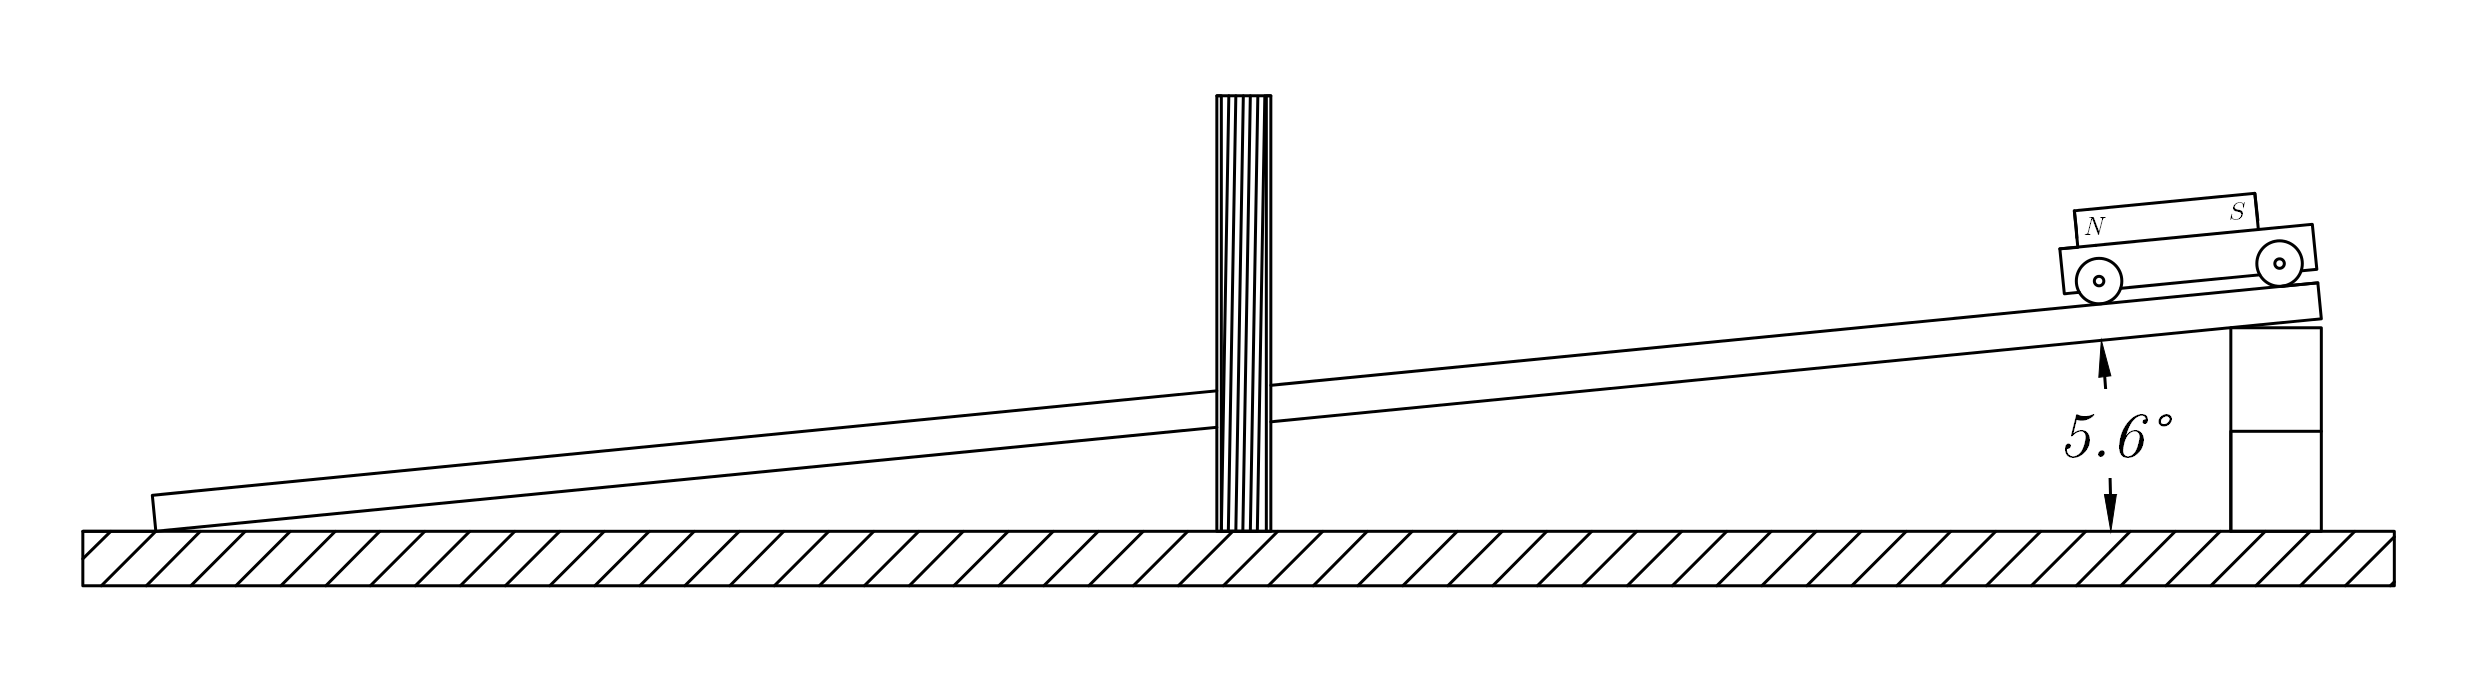
\includegraphics[scale=0.4]{./graphics/physics2lr4.png}
\\\textbf{Figure 1.} The experimental setup.
\end{center}%
\section*{Prediction}
The EMF $\mathcal{E}$ induced across a coil subject to a changing flux is described by Faraday's Law, which describes the EMF as the negative signed derivative of flux (given by $\Phi$):
\begin{equation}
\mathcal{E}_{induced}=-\frac{d\Phi}{dt}
\end{equation}
Magnetic flux is simply considered as the product of the B field normal to some surface and the area of the surface. This is given as follows:
\begin{equation}
\Phi = \int \vec{B}\cdot d \vec{A}
\end{equation}
In this case the surface is given by the plane enclosing the coil, having an area $A$ given by $\pi r^2$, with the surface normal pointing out horizontally. The B field is assumed to be uniform to simplify this derivation. Since the cart moves on the ramp which is fixed at an angle $\theta $ of 5.6$^\circ$ above the horizontal, the B field component in the direction of the coil's normal vector (which is horizontal) is simply $B\cos \theta$, found using trigonometry. Due to the simple geometry and assumed uniform field, the equation for flux can be simplified to $\Phi = B_\perp A$. Plugging this into Faraday's law gives:
\begin{equation}
\mathcal{E} = -\frac{d}{dt}(B_\perp A) = -\frac{d}{dt}(B \cos \theta A) = -A \cos \theta \frac{dB}{dt}
\end{equation} 
Using chain rule, $\frac{dB}{dt}$ can be expanded using $x$ (position along ramp) as an intermediary variable:
\begin{equation}
\mathcal{E}=-A\cos \theta \frac{dB}{dT} = -A \cos\theta \frac{dB}{dx}\frac{dx}{dt}
\end{equation}
$\frac{dx}{dt}$ is the velocity of the cart along the track, so it can be rewritten as $v$. This velocity can be calculated using conservation of energy if $\Delta h$ is known and plugged into \textit{Equation 6}:
\begin{equation}
\frac{1}{2}mv^2=mg\sin\theta\Delta h \longrightarrow v=\sqrt{2g\Delta h\sin\theta}
\end{equation}
\begin{equation}
\mathcal{E}=-A\cos\theta\frac{dB}{dt}v=-A\cos\theta\frac{dB}{dt}\sqrt{2g\Delta h\sin\theta}
\end{equation}
Since $\frac{dB}{dt}$ is too complex to calculate for in this scenario, it is assumed to take constant value. Since all variables other than $\Delta h$ are constants, this means they can be merged into one constant multiplied by the root of $\Delta h$. This value of the constant is unknown, so the relationship between the induced EMF and $\Delta h$ can alternatively be written as a proportionality:
\begin{equation}
\mathcal{E}\propto\sqrt{\Delta h}
\end{equation} 
Therefore, it is predicted that the induced EMF will be proportional to the change in height of the cart at the time it passes through the coil. Since the root of change in height is also proportional to change in velocity, it is expected that the EMF will be proportional to velocity of the cart.
\pagebreak
\section*{Procedure}
First, the angle $\theta$ formed between the ramp and the horizontal was found by measuring the length of the hypotenuse and rise of the ramp. The angle was then calculated using trigonometry. Next, the voltage DAQ device was connected to the terminals of the coil, and a bar magnet was taped to the cart such that one end of the magnet was flush to the front face of the cart. The cart was then put on the track at a position where its front face was 110 cm along the track (up the slope) from the coil. Data acquisition was started on the computer, the cart was released to roll down the ramp, and the acquisition was stopped when the cart had completely passed through the coil. From the acquired data, the peak value for EMF was determined and recorded. This process was again repeated for a distance of 100cm down to 50 cm in 10 cm increments.
\section*{Data}
Below are a table that contains the data for cart displacement and peak EMF observed over each trial and a plot of the change in height versus induced EMF.\vspace{12pt}\\
\title{\textbf{Table 1.}Experimental Displacement and EMF.}
\begin{center}
\renewcommand{\arraystretch}{1.5}
\begin{tabular}{|c|c|c|c|c|c|c|c|}
\hline 
Trial & 1 & 2 & 3 & 4 & 5 & 6 & 7 \\ 
\hline 
$\Delta x$ & 110 cm & 100 cm & 90 cm & 80 cm & 70 cm & 60 cm & 50 cm \\ 
\hline 
$\Delta h$ & 10.7 cm & 9.8 cm & 8.8 cm & 7.8 cm & 6.8 cm & 5.9 cm & 4.9 cm \\ 
\hline 
$\mathcal{E}$ & 0.0675 V & 0.0675 V & 0.0625 V & 0.0575 V & 0.055 V & 0.05 V& 0.0475 V\\ 
\hline 
\end{tabular} 
\end{center}\vspace{6pt}
\title{\textbf{Figure 2.} Induced EMF vs. Change in Height of Cart.}
\begin{center}
    	\resizebox{0.6\textwidth}{!}{% GNUPLOT: LaTeX picture
\setlength{\unitlength}{0.240900pt}
\ifx\plotpoint\undefined\newsavebox{\plotpoint}\fi
\begin{picture}(1500,1200)(0,0)
\sbox{\plotpoint}{\rule[-0.200pt]{0.400pt}{0.400pt}}%
\multiput(212.00,311.58)(0.770,0.500){509}{\rule{0.716pt}{0.120pt}}
\multiput(212.00,310.17)(392.515,256.000){2}{\rule{0.358pt}{0.400pt}}
\multiput(1279.93,419.58)(-2.308,0.499){293}{\rule{1.943pt}{0.120pt}}
\multiput(1283.97,418.17)(-677.967,148.000){2}{\rule{0.972pt}{0.400pt}}
\put(212.0,311.0){\rule[-0.200pt]{0.400pt}{122.859pt}}
\multiput(212.00,311.59)(0.786,0.489){15}{\rule{0.722pt}{0.118pt}}
\multiput(212.00,310.17)(12.501,9.000){2}{\rule{0.361pt}{0.400pt}}
\put(199,293){\makebox(0,0){\tiny 0.15}}
\multiput(603.19,565.93)(-0.728,-0.489){15}{\rule{0.678pt}{0.118pt}}
\multiput(604.59,566.17)(-11.593,-9.000){2}{\rule{0.339pt}{0.400pt}}
\multiput(349.00,282.59)(0.824,0.488){13}{\rule{0.750pt}{0.117pt}}
\multiput(349.00,281.17)(11.443,8.000){2}{\rule{0.375pt}{0.400pt}}
\put(335,264){\makebox(0,0){\tiny 0.16}}
\multiput(740.00,535.93)(-0.786,-0.489){15}{\rule{0.722pt}{0.118pt}}
\multiput(741.50,536.17)(-12.501,-9.000){2}{\rule{0.361pt}{0.400pt}}
\multiput(485.00,252.59)(0.786,0.489){15}{\rule{0.722pt}{0.118pt}}
\multiput(485.00,251.17)(12.501,9.000){2}{\rule{0.361pt}{0.400pt}}
\put(472,234){\makebox(0,0){\tiny 0.17}}
\multiput(875.19,506.93)(-0.728,-0.489){15}{\rule{0.678pt}{0.118pt}}
\multiput(876.59,507.17)(-11.593,-9.000){2}{\rule{0.339pt}{0.400pt}}
\multiput(622.00,223.59)(0.824,0.488){13}{\rule{0.750pt}{0.117pt}}
\multiput(622.00,222.17)(11.443,8.000){2}{\rule{0.375pt}{0.400pt}}
\put(608,205){\makebox(0,0){\tiny 0.18}}
\multiput(1012.00,476.93)(-0.786,-0.489){15}{\rule{0.722pt}{0.118pt}}
\multiput(1013.50,477.17)(-12.501,-9.000){2}{\rule{0.361pt}{0.400pt}}
\multiput(757.00,193.59)(0.786,0.489){15}{\rule{0.722pt}{0.118pt}}
\multiput(757.00,192.17)(12.501,9.000){2}{\rule{0.361pt}{0.400pt}}
\put(745,175){\makebox(0,0){\tiny 0.19}}
\multiput(1148.19,447.93)(-0.728,-0.489){15}{\rule{0.678pt}{0.118pt}}
\multiput(1149.59,448.17)(-11.593,-9.000){2}{\rule{0.339pt}{0.400pt}}
\multiput(894.00,164.59)(0.824,0.488){13}{\rule{0.750pt}{0.117pt}}
\multiput(894.00,163.17)(11.443,8.000){2}{\rule{0.375pt}{0.400pt}}
\put(880,146){\makebox(0,0){\tiny 0.2}}
\multiput(1285.00,417.93)(-0.786,-0.489){15}{\rule{0.722pt}{0.118pt}}
\multiput(1286.50,418.17)(-12.501,-9.000){2}{\rule{0.361pt}{0.400pt}}
\multiput(883.62,164.61)(-3.811,0.447){3}{\rule{2.500pt}{0.108pt}}
\multiput(888.81,163.17)(-12.811,3.000){2}{\rule{1.250pt}{0.400pt}}
\put(911,156){\makebox(0,0){\hspace{0.1in}\tiny 0.12}}
\multiput(212.00,309.94)(2.528,-0.468){5}{\rule{1.900pt}{0.113pt}}
\multiput(212.00,310.17)(14.056,-4.000){2}{\rule{0.950pt}{0.400pt}}
\multiput(935.53,195.60)(-2.382,0.468){5}{\rule{1.800pt}{0.113pt}}
\multiput(939.26,194.17)(-13.264,4.000){2}{\rule{0.900pt}{0.400pt}}
\put(960,188){\makebox(0,0){\hspace{0.1in}\tiny 0.13}}
\multiput(262.00,341.94)(2.382,-0.468){5}{\rule{1.800pt}{0.113pt}}
\multiput(262.00,342.17)(13.264,-4.000){2}{\rule{0.900pt}{0.400pt}}
\multiput(984.53,227.60)(-2.382,0.468){5}{\rule{1.800pt}{0.113pt}}
\multiput(988.26,226.17)(-13.264,4.000){2}{\rule{0.900pt}{0.400pt}}
\put(1010,220){\makebox(0,0){\hspace{0.1in}\tiny 0.14}}
\multiput(311.00,373.94)(2.382,-0.468){5}{\rule{1.800pt}{0.113pt}}
\multiput(311.00,374.17)(13.264,-4.000){2}{\rule{0.900pt}{0.400pt}}
\multiput(1033.53,259.60)(-2.382,0.468){5}{\rule{1.800pt}{0.113pt}}
\multiput(1037.26,258.17)(-13.264,4.000){2}{\rule{0.900pt}{0.400pt}}
\put(1059,252){\makebox(0,0){\hspace{0.1in}\tiny 0.15}}
\multiput(360.00,405.94)(2.382,-0.468){5}{\rule{1.800pt}{0.113pt}}
\multiput(360.00,406.17)(13.264,-4.000){2}{\rule{0.900pt}{0.400pt}}
\multiput(1083.11,291.60)(-2.528,0.468){5}{\rule{1.900pt}{0.113pt}}
\multiput(1087.06,290.17)(-14.056,4.000){2}{\rule{0.950pt}{0.400pt}}
\put(1108,284){\makebox(0,0){\hspace{0.1in}\tiny 0.16}}
\multiput(409.00,437.94)(2.528,-0.468){5}{\rule{1.900pt}{0.113pt}}
\multiput(409.00,438.17)(14.056,-4.000){2}{\rule{0.950pt}{0.400pt}}
\multiput(1132.53,323.60)(-2.382,0.468){5}{\rule{1.800pt}{0.113pt}}
\multiput(1136.26,322.17)(-13.264,4.000){2}{\rule{0.900pt}{0.400pt}}
\put(1157,316){\makebox(0,0){\hspace{0.1in}\tiny 0.17}}
\multiput(459.00,469.94)(2.382,-0.468){5}{\rule{1.800pt}{0.113pt}}
\multiput(459.00,470.17)(13.264,-4.000){2}{\rule{0.900pt}{0.400pt}}
\multiput(1181.53,355.60)(-2.382,0.468){5}{\rule{1.800pt}{0.113pt}}
\multiput(1185.26,354.17)(-13.264,4.000){2}{\rule{0.900pt}{0.400pt}}
\put(1207,347){\makebox(0,0){\hspace{0.1in}\tiny 0.18}}
\multiput(508.00,501.94)(2.382,-0.468){5}{\rule{1.800pt}{0.113pt}}
\multiput(508.00,502.17)(13.264,-4.000){2}{\rule{0.900pt}{0.400pt}}
\multiput(1230.53,387.60)(-2.382,0.468){5}{\rule{1.800pt}{0.113pt}}
\multiput(1234.26,386.17)(-13.264,4.000){2}{\rule{0.900pt}{0.400pt}}
\put(1256,379){\makebox(0,0){\hspace{0.1in}\tiny 0.19}}
\multiput(557.00,533.94)(2.382,-0.468){5}{\rule{1.800pt}{0.113pt}}
\multiput(557.00,534.17)(13.264,-4.000){2}{\rule{0.900pt}{0.400pt}}
\multiput(1280.11,419.60)(-2.528,0.468){5}{\rule{1.900pt}{0.113pt}}
\multiput(1284.06,418.17)(-14.056,4.000){2}{\rule{0.950pt}{0.400pt}}
\put(1305,411){\makebox(0,0){\hspace{0.1in}\tiny 0.2}}
\multiput(606.00,565.94)(2.528,-0.468){5}{\rule{1.900pt}{0.113pt}}
\multiput(606.00,566.17)(14.056,-4.000){2}{\rule{0.950pt}{0.400pt}}
\put(172,481){\makebox(0,0)[r]{\tiny 0}}
\put(212.0,481.0){\rule[-0.200pt]{4.818pt}{0.400pt}}
\put(172,538){\makebox(0,0)[r]{\tiny 0.2}}
\put(212.0,538.0){\rule[-0.200pt]{4.818pt}{0.400pt}}
\put(172,595){\makebox(0,0)[r]{\tiny 0.4}}
\put(212.0,595.0){\rule[-0.200pt]{4.818pt}{0.400pt}}
\put(172,651){\makebox(0,0)[r]{\tiny 0.6}}
\put(212.0,651.0){\rule[-0.200pt]{4.818pt}{0.400pt}}
\put(172,707){\makebox(0,0)[r]{\tiny 0.8}}
\put(212.0,707.0){\rule[-0.200pt]{4.818pt}{0.400pt}}
\put(172,764){\makebox(0,0)[r]{\tiny 1}}
\put(212.0,764.0){\rule[-0.200pt]{4.818pt}{0.400pt}}
\put(172,821){\makebox(0,0)[r]{\tiny 1.2}}
\put(212.0,821.0){\rule[-0.200pt]{4.818pt}{0.400pt}}
\put(72,651){\makebox(0,0){d (meters)\hspace{.5in}}}
\put(212,495.67){\rule{1.686pt}{0.400pt}}
\multiput(212.00,496.17)(3.500,-1.000){2}{\rule{0.843pt}{0.400pt}}
\put(219,494.17){\rule{1.500pt}{0.400pt}}
\multiput(219.00,495.17)(3.887,-2.000){2}{\rule{0.750pt}{0.400pt}}
\put(226,492.67){\rule{1.686pt}{0.400pt}}
\multiput(226.00,493.17)(3.500,-1.000){2}{\rule{0.843pt}{0.400pt}}
\put(233,491.67){\rule{1.686pt}{0.400pt}}
\multiput(233.00,492.17)(3.500,-1.000){2}{\rule{0.843pt}{0.400pt}}
\put(240,490.17){\rule{1.500pt}{0.400pt}}
\multiput(240.00,491.17)(3.887,-2.000){2}{\rule{0.750pt}{0.400pt}}
\put(247,488.67){\rule{1.686pt}{0.400pt}}
\multiput(247.00,489.17)(3.500,-1.000){2}{\rule{0.843pt}{0.400pt}}
\put(254,487.17){\rule{1.500pt}{0.400pt}}
\multiput(254.00,488.17)(3.887,-2.000){2}{\rule{0.750pt}{0.400pt}}
\put(261,485.67){\rule{1.445pt}{0.400pt}}
\multiput(261.00,486.17)(3.000,-1.000){2}{\rule{0.723pt}{0.400pt}}
\put(267,484.17){\rule{1.500pt}{0.400pt}}
\multiput(267.00,485.17)(3.887,-2.000){2}{\rule{0.750pt}{0.400pt}}
\put(274,482.67){\rule{1.686pt}{0.400pt}}
\multiput(274.00,483.17)(3.500,-1.000){2}{\rule{0.843pt}{0.400pt}}
\put(281,481.67){\rule{1.686pt}{0.400pt}}
\multiput(281.00,482.17)(3.500,-1.000){2}{\rule{0.843pt}{0.400pt}}
\put(288,480.17){\rule{1.500pt}{0.400pt}}
\multiput(288.00,481.17)(3.887,-2.000){2}{\rule{0.750pt}{0.400pt}}
\put(295,478.67){\rule{1.686pt}{0.400pt}}
\multiput(295.00,479.17)(3.500,-1.000){2}{\rule{0.843pt}{0.400pt}}
\put(302,477.17){\rule{1.500pt}{0.400pt}}
\multiput(302.00,478.17)(3.887,-2.000){2}{\rule{0.750pt}{0.400pt}}
\put(309,475.67){\rule{1.686pt}{0.400pt}}
\multiput(309.00,476.17)(3.500,-1.000){2}{\rule{0.843pt}{0.400pt}}
\put(316,474.17){\rule{1.500pt}{0.400pt}}
\multiput(316.00,475.17)(3.887,-2.000){2}{\rule{0.750pt}{0.400pt}}
\put(323,472.67){\rule{1.445pt}{0.400pt}}
\multiput(323.00,473.17)(3.000,-1.000){2}{\rule{0.723pt}{0.400pt}}
\put(329,471.17){\rule{1.500pt}{0.400pt}}
\multiput(329.00,472.17)(3.887,-2.000){2}{\rule{0.750pt}{0.400pt}}
\put(336,469.67){\rule{1.686pt}{0.400pt}}
\multiput(336.00,470.17)(3.500,-1.000){2}{\rule{0.843pt}{0.400pt}}
\put(343,468.67){\rule{1.686pt}{0.400pt}}
\multiput(343.00,469.17)(3.500,-1.000){2}{\rule{0.843pt}{0.400pt}}
\put(350,467.17){\rule{1.500pt}{0.400pt}}
\multiput(350.00,468.17)(3.887,-2.000){2}{\rule{0.750pt}{0.400pt}}
\put(357,465.67){\rule{1.686pt}{0.400pt}}
\multiput(357.00,466.17)(3.500,-1.000){2}{\rule{0.843pt}{0.400pt}}
\put(364,464.17){\rule{1.500pt}{0.400pt}}
\multiput(364.00,465.17)(3.887,-2.000){2}{\rule{0.750pt}{0.400pt}}
\put(371,462.67){\rule{1.686pt}{0.400pt}}
\multiput(371.00,463.17)(3.500,-1.000){2}{\rule{0.843pt}{0.400pt}}
\put(378,461.17){\rule{1.500pt}{0.400pt}}
\multiput(378.00,462.17)(3.887,-2.000){2}{\rule{0.750pt}{0.400pt}}
\put(385,459.67){\rule{1.686pt}{0.400pt}}
\multiput(385.00,460.17)(3.500,-1.000){2}{\rule{0.843pt}{0.400pt}}
\put(392,458.67){\rule{1.445pt}{0.400pt}}
\multiput(392.00,459.17)(3.000,-1.000){2}{\rule{0.723pt}{0.400pt}}
\put(398,457.17){\rule{1.500pt}{0.400pt}}
\multiput(398.00,458.17)(3.887,-2.000){2}{\rule{0.750pt}{0.400pt}}
\put(405,455.67){\rule{1.686pt}{0.400pt}}
\multiput(405.00,456.17)(3.500,-1.000){2}{\rule{0.843pt}{0.400pt}}
\put(412,454.17){\rule{1.500pt}{0.400pt}}
\multiput(412.00,455.17)(3.887,-2.000){2}{\rule{0.750pt}{0.400pt}}
\put(419,452.67){\rule{1.686pt}{0.400pt}}
\multiput(419.00,453.17)(3.500,-1.000){2}{\rule{0.843pt}{0.400pt}}
\put(426,451.17){\rule{1.500pt}{0.400pt}}
\multiput(426.00,452.17)(3.887,-2.000){2}{\rule{0.750pt}{0.400pt}}
\put(433,449.67){\rule{1.686pt}{0.400pt}}
\multiput(433.00,450.17)(3.500,-1.000){2}{\rule{0.843pt}{0.400pt}}
\put(440,448.17){\rule{1.500pt}{0.400pt}}
\multiput(440.00,449.17)(3.887,-2.000){2}{\rule{0.750pt}{0.400pt}}
\put(447,446.67){\rule{1.686pt}{0.400pt}}
\multiput(447.00,447.17)(3.500,-1.000){2}{\rule{0.843pt}{0.400pt}}
\put(454,445.67){\rule{1.445pt}{0.400pt}}
\multiput(454.00,446.17)(3.000,-1.000){2}{\rule{0.723pt}{0.400pt}}
\put(460,444.17){\rule{1.500pt}{0.400pt}}
\multiput(460.00,445.17)(3.887,-2.000){2}{\rule{0.750pt}{0.400pt}}
\put(467,442.67){\rule{1.686pt}{0.400pt}}
\multiput(467.00,443.17)(3.500,-1.000){2}{\rule{0.843pt}{0.400pt}}
\put(474,441.17){\rule{1.500pt}{0.400pt}}
\multiput(474.00,442.17)(3.887,-2.000){2}{\rule{0.750pt}{0.400pt}}
\put(481,439.67){\rule{1.686pt}{0.400pt}}
\multiput(481.00,440.17)(3.500,-1.000){2}{\rule{0.843pt}{0.400pt}}
\put(488,438.17){\rule{1.500pt}{0.400pt}}
\multiput(488.00,439.17)(3.887,-2.000){2}{\rule{0.750pt}{0.400pt}}
\put(495,436.67){\rule{1.686pt}{0.400pt}}
\multiput(495.00,437.17)(3.500,-1.000){2}{\rule{0.843pt}{0.400pt}}
\put(502,435.67){\rule{1.686pt}{0.400pt}}
\multiput(502.00,436.17)(3.500,-1.000){2}{\rule{0.843pt}{0.400pt}}
\put(509,434.17){\rule{1.500pt}{0.400pt}}
\multiput(509.00,435.17)(3.887,-2.000){2}{\rule{0.750pt}{0.400pt}}
\put(516,432.67){\rule{1.445pt}{0.400pt}}
\multiput(516.00,433.17)(3.000,-1.000){2}{\rule{0.723pt}{0.400pt}}
\put(522,431.17){\rule{1.500pt}{0.400pt}}
\multiput(522.00,432.17)(3.887,-2.000){2}{\rule{0.750pt}{0.400pt}}
\put(529,429.67){\rule{1.686pt}{0.400pt}}
\multiput(529.00,430.17)(3.500,-1.000){2}{\rule{0.843pt}{0.400pt}}
\put(536,428.17){\rule{1.500pt}{0.400pt}}
\multiput(536.00,429.17)(3.887,-2.000){2}{\rule{0.750pt}{0.400pt}}
\put(543,426.67){\rule{1.686pt}{0.400pt}}
\multiput(543.00,427.17)(3.500,-1.000){2}{\rule{0.843pt}{0.400pt}}
\put(550,425.67){\rule{1.686pt}{0.400pt}}
\multiput(550.00,426.17)(3.500,-1.000){2}{\rule{0.843pt}{0.400pt}}
\put(557,424.17){\rule{1.500pt}{0.400pt}}
\multiput(557.00,425.17)(3.887,-2.000){2}{\rule{0.750pt}{0.400pt}}
\put(564,422.67){\rule{1.686pt}{0.400pt}}
\multiput(564.00,423.17)(3.500,-1.000){2}{\rule{0.843pt}{0.400pt}}
\put(571,421.17){\rule{1.500pt}{0.400pt}}
\multiput(571.00,422.17)(3.887,-2.000){2}{\rule{0.750pt}{0.400pt}}
\put(578,419.67){\rule{1.686pt}{0.400pt}}
\multiput(578.00,420.17)(3.500,-1.000){2}{\rule{0.843pt}{0.400pt}}
\put(585,418.17){\rule{1.300pt}{0.400pt}}
\multiput(585.00,419.17)(3.302,-2.000){2}{\rule{0.650pt}{0.400pt}}
\put(591,416.67){\rule{1.686pt}{0.400pt}}
\multiput(591.00,417.17)(3.500,-1.000){2}{\rule{0.843pt}{0.400pt}}
\put(598,415.17){\rule{1.500pt}{0.400pt}}
\multiput(598.00,416.17)(3.887,-2.000){2}{\rule{0.750pt}{0.400pt}}
\put(605,413.67){\rule{1.686pt}{0.400pt}}
\multiput(605.00,414.17)(3.500,-1.000){2}{\rule{0.843pt}{0.400pt}}
\put(612,412.67){\rule{1.686pt}{0.400pt}}
\multiput(612.00,413.17)(3.500,-1.000){2}{\rule{0.843pt}{0.400pt}}
\put(619,411.17){\rule{1.500pt}{0.400pt}}
\multiput(619.00,412.17)(3.887,-2.000){2}{\rule{0.750pt}{0.400pt}}
\put(626,409.67){\rule{1.686pt}{0.400pt}}
\multiput(626.00,410.17)(3.500,-1.000){2}{\rule{0.843pt}{0.400pt}}
\put(633,408.17){\rule{1.500pt}{0.400pt}}
\multiput(633.00,409.17)(3.887,-2.000){2}{\rule{0.750pt}{0.400pt}}
\put(640,406.67){\rule{1.686pt}{0.400pt}}
\multiput(640.00,407.17)(3.500,-1.000){2}{\rule{0.843pt}{0.400pt}}
\put(647,405.17){\rule{1.300pt}{0.400pt}}
\multiput(647.00,406.17)(3.302,-2.000){2}{\rule{0.650pt}{0.400pt}}
\put(653,403.67){\rule{1.686pt}{0.400pt}}
\multiput(653.00,404.17)(3.500,-1.000){2}{\rule{0.843pt}{0.400pt}}
\put(660,402.67){\rule{1.686pt}{0.400pt}}
\multiput(660.00,403.17)(3.500,-1.000){2}{\rule{0.843pt}{0.400pt}}
\put(667,401.17){\rule{1.500pt}{0.400pt}}
\multiput(667.00,402.17)(3.887,-2.000){2}{\rule{0.750pt}{0.400pt}}
\put(674,399.67){\rule{1.686pt}{0.400pt}}
\multiput(674.00,400.17)(3.500,-1.000){2}{\rule{0.843pt}{0.400pt}}
\put(681,398.17){\rule{1.500pt}{0.400pt}}
\multiput(681.00,399.17)(3.887,-2.000){2}{\rule{0.750pt}{0.400pt}}
\put(688,396.67){\rule{1.686pt}{0.400pt}}
\multiput(688.00,397.17)(3.500,-1.000){2}{\rule{0.843pt}{0.400pt}}
\put(695,395.17){\rule{1.500pt}{0.400pt}}
\multiput(695.00,396.17)(3.887,-2.000){2}{\rule{0.750pt}{0.400pt}}
\put(702,393.67){\rule{1.686pt}{0.400pt}}
\multiput(702.00,394.17)(3.500,-1.000){2}{\rule{0.843pt}{0.400pt}}
\put(709,392.17){\rule{1.300pt}{0.400pt}}
\multiput(709.00,393.17)(3.302,-2.000){2}{\rule{0.650pt}{0.400pt}}
\put(715,390.67){\rule{1.686pt}{0.400pt}}
\multiput(715.00,391.17)(3.500,-1.000){2}{\rule{0.843pt}{0.400pt}}
\put(722,389.67){\rule{1.686pt}{0.400pt}}
\multiput(722.00,390.17)(3.500,-1.000){2}{\rule{0.843pt}{0.400pt}}
\put(729,388.17){\rule{1.500pt}{0.400pt}}
\multiput(729.00,389.17)(3.887,-2.000){2}{\rule{0.750pt}{0.400pt}}
\put(736,386.67){\rule{1.686pt}{0.400pt}}
\multiput(736.00,387.17)(3.500,-1.000){2}{\rule{0.843pt}{0.400pt}}
\put(743,385.17){\rule{1.500pt}{0.400pt}}
\multiput(743.00,386.17)(3.887,-2.000){2}{\rule{0.750pt}{0.400pt}}
\put(750,383.67){\rule{1.445pt}{0.400pt}}
\multiput(750.00,384.17)(3.000,-1.000){2}{\rule{0.723pt}{0.400pt}}
\put(756,382.17){\rule{1.500pt}{0.400pt}}
\multiput(756.00,383.17)(3.887,-2.000){2}{\rule{0.750pt}{0.400pt}}
\put(763,380.67){\rule{1.686pt}{0.400pt}}
\multiput(763.00,381.17)(3.500,-1.000){2}{\rule{0.843pt}{0.400pt}}
\put(770,379.67){\rule{1.686pt}{0.400pt}}
\multiput(770.00,380.17)(3.500,-1.000){2}{\rule{0.843pt}{0.400pt}}
\put(777,378.17){\rule{1.300pt}{0.400pt}}
\multiput(777.00,379.17)(3.302,-2.000){2}{\rule{0.650pt}{0.400pt}}
\put(783,376.67){\rule{1.686pt}{0.400pt}}
\multiput(783.00,377.17)(3.500,-1.000){2}{\rule{0.843pt}{0.400pt}}
\put(790,375.17){\rule{1.500pt}{0.400pt}}
\multiput(790.00,376.17)(3.887,-2.000){2}{\rule{0.750pt}{0.400pt}}
\put(797,373.67){\rule{1.686pt}{0.400pt}}
\multiput(797.00,374.17)(3.500,-1.000){2}{\rule{0.843pt}{0.400pt}}
\put(804,372.17){\rule{1.500pt}{0.400pt}}
\multiput(804.00,373.17)(3.887,-2.000){2}{\rule{0.750pt}{0.400pt}}
\put(811,370.67){\rule{1.686pt}{0.400pt}}
\multiput(811.00,371.17)(3.500,-1.000){2}{\rule{0.843pt}{0.400pt}}
\put(818,369.67){\rule{1.686pt}{0.400pt}}
\multiput(818.00,370.17)(3.500,-1.000){2}{\rule{0.843pt}{0.400pt}}
\put(825,368.17){\rule{1.500pt}{0.400pt}}
\multiput(825.00,369.17)(3.887,-2.000){2}{\rule{0.750pt}{0.400pt}}
\put(832,366.67){\rule{1.686pt}{0.400pt}}
\multiput(832.00,367.17)(3.500,-1.000){2}{\rule{0.843pt}{0.400pt}}
\put(839,365.17){\rule{1.300pt}{0.400pt}}
\multiput(839.00,366.17)(3.302,-2.000){2}{\rule{0.650pt}{0.400pt}}
\put(845,363.67){\rule{1.686pt}{0.400pt}}
\multiput(845.00,364.17)(3.500,-1.000){2}{\rule{0.843pt}{0.400pt}}
\put(852,362.17){\rule{1.500pt}{0.400pt}}
\multiput(852.00,363.17)(3.887,-2.000){2}{\rule{0.750pt}{0.400pt}}
\put(859,360.67){\rule{1.686pt}{0.400pt}}
\multiput(859.00,361.17)(3.500,-1.000){2}{\rule{0.843pt}{0.400pt}}
\put(866,359.17){\rule{1.500pt}{0.400pt}}
\multiput(866.00,360.17)(3.887,-2.000){2}{\rule{0.750pt}{0.400pt}}
\put(873,357.67){\rule{1.686pt}{0.400pt}}
\multiput(873.00,358.17)(3.500,-1.000){2}{\rule{0.843pt}{0.400pt}}
\put(880,356.67){\rule{1.686pt}{0.400pt}}
\multiput(880.00,357.17)(3.500,-1.000){2}{\rule{0.843pt}{0.400pt}}
\put(887,355.17){\rule{1.500pt}{0.400pt}}
\multiput(887.00,356.17)(3.887,-2.000){2}{\rule{0.750pt}{0.400pt}}
\put(256,526.17){\rule{1.500pt}{0.400pt}}
\multiput(256.00,527.17)(3.887,-2.000){2}{\rule{0.750pt}{0.400pt}}
\put(263,524.67){\rule{1.686pt}{0.400pt}}
\multiput(263.00,525.17)(3.500,-1.000){2}{\rule{0.843pt}{0.400pt}}
\put(270,523.17){\rule{1.500pt}{0.400pt}}
\multiput(270.00,524.17)(3.887,-2.000){2}{\rule{0.750pt}{0.400pt}}
\put(277,521.67){\rule{1.686pt}{0.400pt}}
\multiput(277.00,522.17)(3.500,-1.000){2}{\rule{0.843pt}{0.400pt}}
\put(284,520.67){\rule{1.686pt}{0.400pt}}
\multiput(284.00,521.17)(3.500,-1.000){2}{\rule{0.843pt}{0.400pt}}
\put(291,519.17){\rule{1.300pt}{0.400pt}}
\multiput(291.00,520.17)(3.302,-2.000){2}{\rule{0.650pt}{0.400pt}}
\put(297,517.67){\rule{1.686pt}{0.400pt}}
\multiput(297.00,518.17)(3.500,-1.000){2}{\rule{0.843pt}{0.400pt}}
\put(304,516.17){\rule{1.500pt}{0.400pt}}
\multiput(304.00,517.17)(3.887,-2.000){2}{\rule{0.750pt}{0.400pt}}
\put(311,514.67){\rule{1.686pt}{0.400pt}}
\multiput(311.00,515.17)(3.500,-1.000){2}{\rule{0.843pt}{0.400pt}}
\put(318,513.17){\rule{1.500pt}{0.400pt}}
\multiput(318.00,514.17)(3.887,-2.000){2}{\rule{0.750pt}{0.400pt}}
\put(325,511.67){\rule{1.686pt}{0.400pt}}
\multiput(325.00,512.17)(3.500,-1.000){2}{\rule{0.843pt}{0.400pt}}
\put(332,510.67){\rule{1.686pt}{0.400pt}}
\multiput(332.00,511.17)(3.500,-1.000){2}{\rule{0.843pt}{0.400pt}}
\put(339,509.17){\rule{1.500pt}{0.400pt}}
\multiput(339.00,510.17)(3.887,-2.000){2}{\rule{0.750pt}{0.400pt}}
\put(346,507.67){\rule{1.686pt}{0.400pt}}
\multiput(346.00,508.17)(3.500,-1.000){2}{\rule{0.843pt}{0.400pt}}
\put(353,506.17){\rule{1.300pt}{0.400pt}}
\multiput(353.00,507.17)(3.302,-2.000){2}{\rule{0.650pt}{0.400pt}}
\put(359,504.67){\rule{1.686pt}{0.400pt}}
\multiput(359.00,505.17)(3.500,-1.000){2}{\rule{0.843pt}{0.400pt}}
\put(366,503.17){\rule{1.500pt}{0.400pt}}
\multiput(366.00,504.17)(3.887,-2.000){2}{\rule{0.750pt}{0.400pt}}
\put(373,501.67){\rule{1.686pt}{0.400pt}}
\multiput(373.00,502.17)(3.500,-1.000){2}{\rule{0.843pt}{0.400pt}}
\put(380,500.67){\rule{1.686pt}{0.400pt}}
\multiput(380.00,501.17)(3.500,-1.000){2}{\rule{0.843pt}{0.400pt}}
\put(387,499.17){\rule{1.500pt}{0.400pt}}
\multiput(387.00,500.17)(3.887,-2.000){2}{\rule{0.750pt}{0.400pt}}
\put(394,497.67){\rule{1.686pt}{0.400pt}}
\multiput(394.00,498.17)(3.500,-1.000){2}{\rule{0.843pt}{0.400pt}}
\put(401,496.17){\rule{1.500pt}{0.400pt}}
\multiput(401.00,497.17)(3.887,-2.000){2}{\rule{0.750pt}{0.400pt}}
\put(408,494.67){\rule{1.686pt}{0.400pt}}
\multiput(408.00,495.17)(3.500,-1.000){2}{\rule{0.843pt}{0.400pt}}
\put(415,493.17){\rule{1.500pt}{0.400pt}}
\multiput(415.00,494.17)(3.887,-2.000){2}{\rule{0.750pt}{0.400pt}}
\put(422,491.67){\rule{1.445pt}{0.400pt}}
\multiput(422.00,492.17)(3.000,-1.000){2}{\rule{0.723pt}{0.400pt}}
\put(428,490.67){\rule{1.686pt}{0.400pt}}
\multiput(428.00,491.17)(3.500,-1.000){2}{\rule{0.843pt}{0.400pt}}
\put(435,489.17){\rule{1.500pt}{0.400pt}}
\multiput(435.00,490.17)(3.887,-2.000){2}{\rule{0.750pt}{0.400pt}}
\put(442,487.67){\rule{1.686pt}{0.400pt}}
\multiput(442.00,488.17)(3.500,-1.000){2}{\rule{0.843pt}{0.400pt}}
\put(449,486.17){\rule{1.500pt}{0.400pt}}
\multiput(449.00,487.17)(3.887,-2.000){2}{\rule{0.750pt}{0.400pt}}
\put(456,484.67){\rule{1.686pt}{0.400pt}}
\multiput(456.00,485.17)(3.500,-1.000){2}{\rule{0.843pt}{0.400pt}}
\put(463,483.17){\rule{1.500pt}{0.400pt}}
\multiput(463.00,484.17)(3.887,-2.000){2}{\rule{0.750pt}{0.400pt}}
\put(470,481.67){\rule{1.686pt}{0.400pt}}
\multiput(470.00,482.17)(3.500,-1.000){2}{\rule{0.843pt}{0.400pt}}
\put(477,480.67){\rule{1.686pt}{0.400pt}}
\multiput(477.00,481.17)(3.500,-1.000){2}{\rule{0.843pt}{0.400pt}}
\put(484,479.17){\rule{1.300pt}{0.400pt}}
\multiput(484.00,480.17)(3.302,-2.000){2}{\rule{0.650pt}{0.400pt}}
\put(490,477.67){\rule{1.686pt}{0.400pt}}
\multiput(490.00,478.17)(3.500,-1.000){2}{\rule{0.843pt}{0.400pt}}
\put(497,476.17){\rule{1.500pt}{0.400pt}}
\multiput(497.00,477.17)(3.887,-2.000){2}{\rule{0.750pt}{0.400pt}}
\put(504,474.67){\rule{1.686pt}{0.400pt}}
\multiput(504.00,475.17)(3.500,-1.000){2}{\rule{0.843pt}{0.400pt}}
\put(511,473.17){\rule{1.500pt}{0.400pt}}
\multiput(511.00,474.17)(3.887,-2.000){2}{\rule{0.750pt}{0.400pt}}
\put(518,471.67){\rule{1.686pt}{0.400pt}}
\multiput(518.00,472.17)(3.500,-1.000){2}{\rule{0.843pt}{0.400pt}}
\put(525,470.67){\rule{1.686pt}{0.400pt}}
\multiput(525.00,471.17)(3.500,-1.000){2}{\rule{0.843pt}{0.400pt}}
\put(532,469.17){\rule{1.500pt}{0.400pt}}
\multiput(532.00,470.17)(3.887,-2.000){2}{\rule{0.750pt}{0.400pt}}
\put(539,467.67){\rule{1.686pt}{0.400pt}}
\multiput(539.00,468.17)(3.500,-1.000){2}{\rule{0.843pt}{0.400pt}}
\put(546,466.17){\rule{1.300pt}{0.400pt}}
\multiput(546.00,467.17)(3.302,-2.000){2}{\rule{0.650pt}{0.400pt}}
\put(552,464.67){\rule{1.686pt}{0.400pt}}
\multiput(552.00,465.17)(3.500,-1.000){2}{\rule{0.843pt}{0.400pt}}
\put(559,463.17){\rule{1.500pt}{0.400pt}}
\multiput(559.00,464.17)(3.887,-2.000){2}{\rule{0.750pt}{0.400pt}}
\put(566,461.67){\rule{1.686pt}{0.400pt}}
\multiput(566.00,462.17)(3.500,-1.000){2}{\rule{0.843pt}{0.400pt}}
\put(573,460.17){\rule{1.500pt}{0.400pt}}
\multiput(573.00,461.17)(3.887,-2.000){2}{\rule{0.750pt}{0.400pt}}
\put(580,458.67){\rule{1.686pt}{0.400pt}}
\multiput(580.00,459.17)(3.500,-1.000){2}{\rule{0.843pt}{0.400pt}}
\put(587,457.67){\rule{1.686pt}{0.400pt}}
\multiput(587.00,458.17)(3.500,-1.000){2}{\rule{0.843pt}{0.400pt}}
\put(594,456.17){\rule{1.500pt}{0.400pt}}
\multiput(594.00,457.17)(3.887,-2.000){2}{\rule{0.750pt}{0.400pt}}
\put(601,454.67){\rule{1.686pt}{0.400pt}}
\multiput(601.00,455.17)(3.500,-1.000){2}{\rule{0.843pt}{0.400pt}}
\put(608,453.17){\rule{1.500pt}{0.400pt}}
\multiput(608.00,454.17)(3.887,-2.000){2}{\rule{0.750pt}{0.400pt}}
\put(615,451.67){\rule{1.445pt}{0.400pt}}
\multiput(615.00,452.17)(3.000,-1.000){2}{\rule{0.723pt}{0.400pt}}
\put(621,450.17){\rule{1.500pt}{0.400pt}}
\multiput(621.00,451.17)(3.887,-2.000){2}{\rule{0.750pt}{0.400pt}}
\put(628,448.67){\rule{1.686pt}{0.400pt}}
\multiput(628.00,449.17)(3.500,-1.000){2}{\rule{0.843pt}{0.400pt}}
\put(635,447.67){\rule{1.686pt}{0.400pt}}
\multiput(635.00,448.17)(3.500,-1.000){2}{\rule{0.843pt}{0.400pt}}
\put(642,446.17){\rule{1.500pt}{0.400pt}}
\multiput(642.00,447.17)(3.887,-2.000){2}{\rule{0.750pt}{0.400pt}}
\put(649,444.67){\rule{1.686pt}{0.400pt}}
\multiput(649.00,445.17)(3.500,-1.000){2}{\rule{0.843pt}{0.400pt}}
\put(656,443.17){\rule{1.500pt}{0.400pt}}
\multiput(656.00,444.17)(3.887,-2.000){2}{\rule{0.750pt}{0.400pt}}
\put(663,441.67){\rule{1.686pt}{0.400pt}}
\multiput(663.00,442.17)(3.500,-1.000){2}{\rule{0.843pt}{0.400pt}}
\put(670,440.17){\rule{1.500pt}{0.400pt}}
\multiput(670.00,441.17)(3.887,-2.000){2}{\rule{0.750pt}{0.400pt}}
\put(677,438.67){\rule{1.445pt}{0.400pt}}
\multiput(677.00,439.17)(3.000,-1.000){2}{\rule{0.723pt}{0.400pt}}
\put(683,437.67){\rule{1.686pt}{0.400pt}}
\multiput(683.00,438.17)(3.500,-1.000){2}{\rule{0.843pt}{0.400pt}}
\put(690,436.17){\rule{1.500pt}{0.400pt}}
\multiput(690.00,437.17)(3.887,-2.000){2}{\rule{0.750pt}{0.400pt}}
\put(697,434.67){\rule{1.686pt}{0.400pt}}
\multiput(697.00,435.17)(3.500,-1.000){2}{\rule{0.843pt}{0.400pt}}
\put(704,433.17){\rule{1.500pt}{0.400pt}}
\multiput(704.00,434.17)(3.887,-2.000){2}{\rule{0.750pt}{0.400pt}}
\put(711,431.67){\rule{1.686pt}{0.400pt}}
\multiput(711.00,432.17)(3.500,-1.000){2}{\rule{0.843pt}{0.400pt}}
\put(718,430.17){\rule{1.500pt}{0.400pt}}
\multiput(718.00,431.17)(3.887,-2.000){2}{\rule{0.750pt}{0.400pt}}
\put(725,428.67){\rule{1.686pt}{0.400pt}}
\multiput(725.00,429.17)(3.500,-1.000){2}{\rule{0.843pt}{0.400pt}}
\put(732,427.67){\rule{1.686pt}{0.400pt}}
\multiput(732.00,428.17)(3.500,-1.000){2}{\rule{0.843pt}{0.400pt}}
\put(739,426.17){\rule{1.300pt}{0.400pt}}
\multiput(739.00,427.17)(3.302,-2.000){2}{\rule{0.650pt}{0.400pt}}
\put(745,424.67){\rule{1.445pt}{0.400pt}}
\multiput(745.00,425.17)(3.000,-1.000){2}{\rule{0.723pt}{0.400pt}}
\put(751,423.17){\rule{1.500pt}{0.400pt}}
\multiput(751.00,424.17)(3.887,-2.000){2}{\rule{0.750pt}{0.400pt}}
\put(758,421.67){\rule{1.686pt}{0.400pt}}
\multiput(758.00,422.17)(3.500,-1.000){2}{\rule{0.843pt}{0.400pt}}
\put(765,420.17){\rule{1.500pt}{0.400pt}}
\multiput(765.00,421.17)(3.887,-2.000){2}{\rule{0.750pt}{0.400pt}}
\put(772,418.67){\rule{1.686pt}{0.400pt}}
\multiput(772.00,419.17)(3.500,-1.000){2}{\rule{0.843pt}{0.400pt}}
\put(779,417.67){\rule{1.686pt}{0.400pt}}
\multiput(779.00,418.17)(3.500,-1.000){2}{\rule{0.843pt}{0.400pt}}
\put(786,416.17){\rule{1.500pt}{0.400pt}}
\multiput(786.00,417.17)(3.887,-2.000){2}{\rule{0.750pt}{0.400pt}}
\put(793,414.67){\rule{1.686pt}{0.400pt}}
\multiput(793.00,415.17)(3.500,-1.000){2}{\rule{0.843pt}{0.400pt}}
\put(800,413.17){\rule{1.500pt}{0.400pt}}
\multiput(800.00,414.17)(3.887,-2.000){2}{\rule{0.750pt}{0.400pt}}
\put(807,411.67){\rule{1.445pt}{0.400pt}}
\multiput(807.00,412.17)(3.000,-1.000){2}{\rule{0.723pt}{0.400pt}}
\put(813,410.17){\rule{1.500pt}{0.400pt}}
\multiput(813.00,411.17)(3.887,-2.000){2}{\rule{0.750pt}{0.400pt}}
\put(820,408.67){\rule{1.686pt}{0.400pt}}
\multiput(820.00,409.17)(3.500,-1.000){2}{\rule{0.843pt}{0.400pt}}
\put(827,407.67){\rule{1.686pt}{0.400pt}}
\multiput(827.00,408.17)(3.500,-1.000){2}{\rule{0.843pt}{0.400pt}}
\put(834,406.17){\rule{1.500pt}{0.400pt}}
\multiput(834.00,407.17)(3.887,-2.000){2}{\rule{0.750pt}{0.400pt}}
\put(841,404.67){\rule{1.686pt}{0.400pt}}
\multiput(841.00,405.17)(3.500,-1.000){2}{\rule{0.843pt}{0.400pt}}
\put(848,403.17){\rule{1.500pt}{0.400pt}}
\multiput(848.00,404.17)(3.887,-2.000){2}{\rule{0.750pt}{0.400pt}}
\put(855,401.67){\rule{1.686pt}{0.400pt}}
\multiput(855.00,402.17)(3.500,-1.000){2}{\rule{0.843pt}{0.400pt}}
\put(862,400.17){\rule{1.500pt}{0.400pt}}
\multiput(862.00,401.17)(3.887,-2.000){2}{\rule{0.750pt}{0.400pt}}
\put(869,398.67){\rule{1.445pt}{0.400pt}}
\multiput(869.00,399.17)(3.000,-1.000){2}{\rule{0.723pt}{0.400pt}}
\put(875,397.67){\rule{1.686pt}{0.400pt}}
\multiput(875.00,398.17)(3.500,-1.000){2}{\rule{0.843pt}{0.400pt}}
\put(882,396.17){\rule{1.500pt}{0.400pt}}
\multiput(882.00,397.17)(3.887,-2.000){2}{\rule{0.750pt}{0.400pt}}
\put(889,394.67){\rule{1.686pt}{0.400pt}}
\multiput(889.00,395.17)(3.500,-1.000){2}{\rule{0.843pt}{0.400pt}}
\put(896,393.17){\rule{1.500pt}{0.400pt}}
\multiput(896.00,394.17)(3.887,-2.000){2}{\rule{0.750pt}{0.400pt}}
\put(903,391.67){\rule{1.686pt}{0.400pt}}
\multiput(903.00,392.17)(3.500,-1.000){2}{\rule{0.843pt}{0.400pt}}
\put(910,390.17){\rule{1.500pt}{0.400pt}}
\multiput(910.00,391.17)(3.887,-2.000){2}{\rule{0.750pt}{0.400pt}}
\put(917,388.67){\rule{1.686pt}{0.400pt}}
\multiput(917.00,389.17)(3.500,-1.000){2}{\rule{0.843pt}{0.400pt}}
\put(924,387.67){\rule{1.686pt}{0.400pt}}
\multiput(924.00,388.17)(3.500,-1.000){2}{\rule{0.843pt}{0.400pt}}
\put(931,386.17){\rule{1.300pt}{0.400pt}}
\multiput(931.00,387.17)(3.302,-2.000){2}{\rule{0.650pt}{0.400pt}}
\put(300,556.67){\rule{1.686pt}{0.400pt}}
\multiput(300.00,557.17)(3.500,-1.000){2}{\rule{0.843pt}{0.400pt}}
\put(307,555.67){\rule{1.686pt}{0.400pt}}
\multiput(307.00,556.17)(3.500,-1.000){2}{\rule{0.843pt}{0.400pt}}
\put(314,554.17){\rule{1.500pt}{0.400pt}}
\multiput(314.00,555.17)(3.887,-2.000){2}{\rule{0.750pt}{0.400pt}}
\put(321,552.67){\rule{1.445pt}{0.400pt}}
\multiput(321.00,553.17)(3.000,-1.000){2}{\rule{0.723pt}{0.400pt}}
\put(327,551.17){\rule{1.500pt}{0.400pt}}
\multiput(327.00,552.17)(3.887,-2.000){2}{\rule{0.750pt}{0.400pt}}
\put(334,549.67){\rule{1.686pt}{0.400pt}}
\multiput(334.00,550.17)(3.500,-1.000){2}{\rule{0.843pt}{0.400pt}}
\put(341,548.17){\rule{1.500pt}{0.400pt}}
\multiput(341.00,549.17)(3.887,-2.000){2}{\rule{0.750pt}{0.400pt}}
\put(348,546.67){\rule{1.686pt}{0.400pt}}
\multiput(348.00,547.17)(3.500,-1.000){2}{\rule{0.843pt}{0.400pt}}
\put(355,545.67){\rule{1.686pt}{0.400pt}}
\multiput(355.00,546.17)(3.500,-1.000){2}{\rule{0.843pt}{0.400pt}}
\put(362,544.17){\rule{1.500pt}{0.400pt}}
\multiput(362.00,545.17)(3.887,-2.000){2}{\rule{0.750pt}{0.400pt}}
\put(369,542.67){\rule{1.686pt}{0.400pt}}
\multiput(369.00,543.17)(3.500,-1.000){2}{\rule{0.843pt}{0.400pt}}
\put(376,541.17){\rule{1.500pt}{0.400pt}}
\multiput(376.00,542.17)(3.887,-2.000){2}{\rule{0.750pt}{0.400pt}}
\put(383,539.67){\rule{1.445pt}{0.400pt}}
\multiput(383.00,540.17)(3.000,-1.000){2}{\rule{0.723pt}{0.400pt}}
\put(389,538.17){\rule{1.500pt}{0.400pt}}
\multiput(389.00,539.17)(3.887,-2.000){2}{\rule{0.750pt}{0.400pt}}
\put(396,536.67){\rule{1.686pt}{0.400pt}}
\multiput(396.00,537.17)(3.500,-1.000){2}{\rule{0.843pt}{0.400pt}}
\put(403,535.67){\rule{1.686pt}{0.400pt}}
\multiput(403.00,536.17)(3.500,-1.000){2}{\rule{0.843pt}{0.400pt}}
\put(410,534.17){\rule{1.500pt}{0.400pt}}
\multiput(410.00,535.17)(3.887,-2.000){2}{\rule{0.750pt}{0.400pt}}
\put(417,532.67){\rule{1.686pt}{0.400pt}}
\multiput(417.00,533.17)(3.500,-1.000){2}{\rule{0.843pt}{0.400pt}}
\put(424,531.17){\rule{1.500pt}{0.400pt}}
\multiput(424.00,532.17)(3.887,-2.000){2}{\rule{0.750pt}{0.400pt}}
\put(431,529.67){\rule{1.686pt}{0.400pt}}
\multiput(431.00,530.17)(3.500,-1.000){2}{\rule{0.843pt}{0.400pt}}
\put(438,528.67){\rule{1.686pt}{0.400pt}}
\multiput(438.00,529.17)(3.500,-1.000){2}{\rule{0.843pt}{0.400pt}}
\put(445,527.17){\rule{1.300pt}{0.400pt}}
\multiput(445.00,528.17)(3.302,-2.000){2}{\rule{0.650pt}{0.400pt}}
\put(451,525.67){\rule{1.686pt}{0.400pt}}
\multiput(451.00,526.17)(3.500,-1.000){2}{\rule{0.843pt}{0.400pt}}
\put(458,524.17){\rule{1.500pt}{0.400pt}}
\multiput(458.00,525.17)(3.887,-2.000){2}{\rule{0.750pt}{0.400pt}}
\put(465,522.67){\rule{1.686pt}{0.400pt}}
\multiput(465.00,523.17)(3.500,-1.000){2}{\rule{0.843pt}{0.400pt}}
\put(472,521.17){\rule{1.500pt}{0.400pt}}
\multiput(472.00,522.17)(3.887,-2.000){2}{\rule{0.750pt}{0.400pt}}
\put(479,519.67){\rule{1.686pt}{0.400pt}}
\multiput(479.00,520.17)(3.500,-1.000){2}{\rule{0.843pt}{0.400pt}}
\put(486,518.67){\rule{1.686pt}{0.400pt}}
\multiput(486.00,519.17)(3.500,-1.000){2}{\rule{0.843pt}{0.400pt}}
\put(493,517.17){\rule{1.500pt}{0.400pt}}
\multiput(493.00,518.17)(3.887,-2.000){2}{\rule{0.750pt}{0.400pt}}
\put(500,515.67){\rule{1.686pt}{0.400pt}}
\multiput(500.00,516.17)(3.500,-1.000){2}{\rule{0.843pt}{0.400pt}}
\put(507,514.17){\rule{1.500pt}{0.400pt}}
\multiput(507.00,515.17)(3.887,-2.000){2}{\rule{0.750pt}{0.400pt}}
\put(514,512.67){\rule{1.445pt}{0.400pt}}
\multiput(514.00,513.17)(3.000,-1.000){2}{\rule{0.723pt}{0.400pt}}
\put(520,511.17){\rule{1.500pt}{0.400pt}}
\multiput(520.00,512.17)(3.887,-2.000){2}{\rule{0.750pt}{0.400pt}}
\put(527,509.67){\rule{1.686pt}{0.400pt}}
\multiput(527.00,510.17)(3.500,-1.000){2}{\rule{0.843pt}{0.400pt}}
\put(534,508.67){\rule{1.686pt}{0.400pt}}
\multiput(534.00,509.17)(3.500,-1.000){2}{\rule{0.843pt}{0.400pt}}
\put(541,507.17){\rule{1.500pt}{0.400pt}}
\multiput(541.00,508.17)(3.887,-2.000){2}{\rule{0.750pt}{0.400pt}}
\put(548,505.67){\rule{1.686pt}{0.400pt}}
\multiput(548.00,506.17)(3.500,-1.000){2}{\rule{0.843pt}{0.400pt}}
\put(555,504.17){\rule{1.500pt}{0.400pt}}
\multiput(555.00,505.17)(3.887,-2.000){2}{\rule{0.750pt}{0.400pt}}
\put(562,502.67){\rule{1.686pt}{0.400pt}}
\multiput(562.00,503.17)(3.500,-1.000){2}{\rule{0.843pt}{0.400pt}}
\put(569,501.17){\rule{1.500pt}{0.400pt}}
\multiput(569.00,502.17)(3.887,-2.000){2}{\rule{0.750pt}{0.400pt}}
\put(576,499.67){\rule{1.445pt}{0.400pt}}
\multiput(576.00,500.17)(3.000,-1.000){2}{\rule{0.723pt}{0.400pt}}
\put(582,498.67){\rule{1.686pt}{0.400pt}}
\multiput(582.00,499.17)(3.500,-1.000){2}{\rule{0.843pt}{0.400pt}}
\put(589,497.17){\rule{1.500pt}{0.400pt}}
\multiput(589.00,498.17)(3.887,-2.000){2}{\rule{0.750pt}{0.400pt}}
\put(596,495.67){\rule{1.686pt}{0.400pt}}
\multiput(596.00,496.17)(3.500,-1.000){2}{\rule{0.843pt}{0.400pt}}
\put(603,494.17){\rule{1.500pt}{0.400pt}}
\multiput(603.00,495.17)(3.887,-2.000){2}{\rule{0.750pt}{0.400pt}}
\put(610,492.67){\rule{1.686pt}{0.400pt}}
\multiput(610.00,493.17)(3.500,-1.000){2}{\rule{0.843pt}{0.400pt}}
\put(617,491.67){\rule{1.686pt}{0.400pt}}
\multiput(617.00,492.17)(3.500,-1.000){2}{\rule{0.843pt}{0.400pt}}
\put(624,490.17){\rule{1.500pt}{0.400pt}}
\multiput(624.00,491.17)(3.887,-2.000){2}{\rule{0.750pt}{0.400pt}}
\put(631,488.67){\rule{1.686pt}{0.400pt}}
\multiput(631.00,489.17)(3.500,-1.000){2}{\rule{0.843pt}{0.400pt}}
\put(638,487.17){\rule{1.500pt}{0.400pt}}
\multiput(638.00,488.17)(3.887,-2.000){2}{\rule{0.750pt}{0.400pt}}
\put(645,485.67){\rule{1.445pt}{0.400pt}}
\multiput(645.00,486.17)(3.000,-1.000){2}{\rule{0.723pt}{0.400pt}}
\put(651,484.17){\rule{1.500pt}{0.400pt}}
\multiput(651.00,485.17)(3.887,-2.000){2}{\rule{0.750pt}{0.400pt}}
\put(658,482.67){\rule{1.686pt}{0.400pt}}
\multiput(658.00,483.17)(3.500,-1.000){2}{\rule{0.843pt}{0.400pt}}
\put(665,481.67){\rule{1.686pt}{0.400pt}}
\multiput(665.00,482.17)(3.500,-1.000){2}{\rule{0.843pt}{0.400pt}}
\put(672,480.17){\rule{1.500pt}{0.400pt}}
\multiput(672.00,481.17)(3.887,-2.000){2}{\rule{0.750pt}{0.400pt}}
\put(679,478.67){\rule{1.686pt}{0.400pt}}
\multiput(679.00,479.17)(3.500,-1.000){2}{\rule{0.843pt}{0.400pt}}
\put(686,477.17){\rule{1.500pt}{0.400pt}}
\multiput(686.00,478.17)(3.887,-2.000){2}{\rule{0.750pt}{0.400pt}}
\put(693,475.67){\rule{1.686pt}{0.400pt}}
\multiput(693.00,476.17)(3.500,-1.000){2}{\rule{0.843pt}{0.400pt}}
\put(700,474.17){\rule{1.500pt}{0.400pt}}
\multiput(700.00,475.17)(3.887,-2.000){2}{\rule{0.750pt}{0.400pt}}
\put(707,472.67){\rule{1.445pt}{0.400pt}}
\multiput(707.00,473.17)(3.000,-1.000){2}{\rule{0.723pt}{0.400pt}}
\put(713,471.67){\rule{1.686pt}{0.400pt}}
\multiput(713.00,472.17)(3.500,-1.000){2}{\rule{0.843pt}{0.400pt}}
\put(720,470.17){\rule{1.500pt}{0.400pt}}
\multiput(720.00,471.17)(3.887,-2.000){2}{\rule{0.750pt}{0.400pt}}
\put(727,468.67){\rule{1.686pt}{0.400pt}}
\multiput(727.00,469.17)(3.500,-1.000){2}{\rule{0.843pt}{0.400pt}}
\put(734,467.17){\rule{1.500pt}{0.400pt}}
\multiput(734.00,468.17)(3.887,-2.000){2}{\rule{0.750pt}{0.400pt}}
\put(741,465.67){\rule{1.686pt}{0.400pt}}
\multiput(741.00,466.17)(3.500,-1.000){2}{\rule{0.843pt}{0.400pt}}
\put(748,464.67){\rule{1.445pt}{0.400pt}}
\multiput(748.00,465.17)(3.000,-1.000){2}{\rule{0.723pt}{0.400pt}}
\put(754,463.17){\rule{1.500pt}{0.400pt}}
\multiput(754.00,464.17)(3.887,-2.000){2}{\rule{0.750pt}{0.400pt}}
\put(761,461.67){\rule{1.686pt}{0.400pt}}
\multiput(761.00,462.17)(3.500,-1.000){2}{\rule{0.843pt}{0.400pt}}
\put(768,460.17){\rule{1.300pt}{0.400pt}}
\multiput(768.00,461.17)(3.302,-2.000){2}{\rule{0.650pt}{0.400pt}}
\put(774,458.67){\rule{1.686pt}{0.400pt}}
\multiput(774.00,459.17)(3.500,-1.000){2}{\rule{0.843pt}{0.400pt}}
\put(781,457.17){\rule{1.500pt}{0.400pt}}
\multiput(781.00,458.17)(3.887,-2.000){2}{\rule{0.750pt}{0.400pt}}
\put(788,455.67){\rule{1.686pt}{0.400pt}}
\multiput(788.00,456.17)(3.500,-1.000){2}{\rule{0.843pt}{0.400pt}}
\put(795,454.67){\rule{1.686pt}{0.400pt}}
\multiput(795.00,455.17)(3.500,-1.000){2}{\rule{0.843pt}{0.400pt}}
\put(802,453.17){\rule{1.500pt}{0.400pt}}
\multiput(802.00,454.17)(3.887,-2.000){2}{\rule{0.750pt}{0.400pt}}
\put(809,451.67){\rule{1.686pt}{0.400pt}}
\multiput(809.00,452.17)(3.500,-1.000){2}{\rule{0.843pt}{0.400pt}}
\put(816,450.17){\rule{1.500pt}{0.400pt}}
\multiput(816.00,451.17)(3.887,-2.000){2}{\rule{0.750pt}{0.400pt}}
\put(823,448.67){\rule{1.686pt}{0.400pt}}
\multiput(823.00,449.17)(3.500,-1.000){2}{\rule{0.843pt}{0.400pt}}
\put(830,447.17){\rule{1.500pt}{0.400pt}}
\multiput(830.00,448.17)(3.887,-2.000){2}{\rule{0.750pt}{0.400pt}}
\put(837,445.67){\rule{1.445pt}{0.400pt}}
\multiput(837.00,446.17)(3.000,-1.000){2}{\rule{0.723pt}{0.400pt}}
\put(843,444.67){\rule{1.686pt}{0.400pt}}
\multiput(843.00,445.17)(3.500,-1.000){2}{\rule{0.843pt}{0.400pt}}
\put(850,443.17){\rule{1.500pt}{0.400pt}}
\multiput(850.00,444.17)(3.887,-2.000){2}{\rule{0.750pt}{0.400pt}}
\put(857,441.67){\rule{1.686pt}{0.400pt}}
\multiput(857.00,442.17)(3.500,-1.000){2}{\rule{0.843pt}{0.400pt}}
\put(864,440.17){\rule{1.500pt}{0.400pt}}
\multiput(864.00,441.17)(3.887,-2.000){2}{\rule{0.750pt}{0.400pt}}
\put(871,438.67){\rule{1.686pt}{0.400pt}}
\multiput(871.00,439.17)(3.500,-1.000){2}{\rule{0.843pt}{0.400pt}}
\put(878,437.67){\rule{1.686pt}{0.400pt}}
\multiput(878.00,438.17)(3.500,-1.000){2}{\rule{0.843pt}{0.400pt}}
\put(885,436.17){\rule{1.500pt}{0.400pt}}
\multiput(885.00,437.17)(3.887,-2.000){2}{\rule{0.750pt}{0.400pt}}
\put(892,434.67){\rule{1.686pt}{0.400pt}}
\multiput(892.00,435.17)(3.500,-1.000){2}{\rule{0.843pt}{0.400pt}}
\put(899,433.17){\rule{1.300pt}{0.400pt}}
\multiput(899.00,434.17)(3.302,-2.000){2}{\rule{0.650pt}{0.400pt}}
\put(905,431.67){\rule{1.686pt}{0.400pt}}
\multiput(905.00,432.17)(3.500,-1.000){2}{\rule{0.843pt}{0.400pt}}
\put(912,430.17){\rule{1.500pt}{0.400pt}}
\multiput(912.00,431.17)(3.887,-2.000){2}{\rule{0.750pt}{0.400pt}}
\put(919,428.67){\rule{1.686pt}{0.400pt}}
\multiput(919.00,429.17)(3.500,-1.000){2}{\rule{0.843pt}{0.400pt}}
\put(926,427.67){\rule{1.686pt}{0.400pt}}
\multiput(926.00,428.17)(3.500,-1.000){2}{\rule{0.843pt}{0.400pt}}
\put(933,426.17){\rule{1.500pt}{0.400pt}}
\multiput(933.00,427.17)(3.887,-2.000){2}{\rule{0.750pt}{0.400pt}}
\put(940,424.67){\rule{1.686pt}{0.400pt}}
\multiput(940.00,425.17)(3.500,-1.000){2}{\rule{0.843pt}{0.400pt}}
\put(947,423.17){\rule{1.500pt}{0.400pt}}
\multiput(947.00,424.17)(3.887,-2.000){2}{\rule{0.750pt}{0.400pt}}
\put(954,421.67){\rule{1.686pt}{0.400pt}}
\multiput(954.00,422.17)(3.500,-1.000){2}{\rule{0.843pt}{0.400pt}}
\put(961,420.17){\rule{1.300pt}{0.400pt}}
\multiput(961.00,421.17)(3.302,-2.000){2}{\rule{0.650pt}{0.400pt}}
\put(967,418.67){\rule{1.686pt}{0.400pt}}
\multiput(967.00,419.17)(3.500,-1.000){2}{\rule{0.843pt}{0.400pt}}
\put(974,417.67){\rule{1.686pt}{0.400pt}}
\multiput(974.00,418.17)(3.500,-1.000){2}{\rule{0.843pt}{0.400pt}}
\put(344,587.67){\rule{1.686pt}{0.400pt}}
\multiput(344.00,588.17)(3.500,-1.000){2}{\rule{0.843pt}{0.400pt}}
\put(351,586.67){\rule{1.445pt}{0.400pt}}
\multiput(351.00,587.17)(3.000,-1.000){2}{\rule{0.723pt}{0.400pt}}
\put(357,585.17){\rule{1.500pt}{0.400pt}}
\multiput(357.00,586.17)(3.887,-2.000){2}{\rule{0.750pt}{0.400pt}}
\put(364,583.67){\rule{1.686pt}{0.400pt}}
\multiput(364.00,584.17)(3.500,-1.000){2}{\rule{0.843pt}{0.400pt}}
\put(371,582.17){\rule{1.500pt}{0.400pt}}
\multiput(371.00,583.17)(3.887,-2.000){2}{\rule{0.750pt}{0.400pt}}
\put(378,580.67){\rule{1.686pt}{0.400pt}}
\multiput(378.00,581.17)(3.500,-1.000){2}{\rule{0.843pt}{0.400pt}}
\put(385,579.67){\rule{1.686pt}{0.400pt}}
\multiput(385.00,580.17)(3.500,-1.000){2}{\rule{0.843pt}{0.400pt}}
\put(392,578.17){\rule{1.500pt}{0.400pt}}
\multiput(392.00,579.17)(3.887,-2.000){2}{\rule{0.750pt}{0.400pt}}
\put(399,576.67){\rule{1.686pt}{0.400pt}}
\multiput(399.00,577.17)(3.500,-1.000){2}{\rule{0.843pt}{0.400pt}}
\put(406,575.17){\rule{1.500pt}{0.400pt}}
\multiput(406.00,576.17)(3.887,-2.000){2}{\rule{0.750pt}{0.400pt}}
\put(413,573.67){\rule{1.445pt}{0.400pt}}
\multiput(413.00,574.17)(3.000,-1.000){2}{\rule{0.723pt}{0.400pt}}
\put(419,572.67){\rule{1.686pt}{0.400pt}}
\multiput(419.00,573.17)(3.500,-1.000){2}{\rule{0.843pt}{0.400pt}}
\put(426,571.17){\rule{1.500pt}{0.400pt}}
\multiput(426.00,572.17)(3.887,-2.000){2}{\rule{0.750pt}{0.400pt}}
\put(433,569.67){\rule{1.686pt}{0.400pt}}
\multiput(433.00,570.17)(3.500,-1.000){2}{\rule{0.843pt}{0.400pt}}
\put(440,568.17){\rule{1.500pt}{0.400pt}}
\multiput(440.00,569.17)(3.887,-2.000){2}{\rule{0.750pt}{0.400pt}}
\put(447,566.67){\rule{1.686pt}{0.400pt}}
\multiput(447.00,567.17)(3.500,-1.000){2}{\rule{0.843pt}{0.400pt}}
\put(454,565.17){\rule{1.500pt}{0.400pt}}
\multiput(454.00,566.17)(3.887,-2.000){2}{\rule{0.750pt}{0.400pt}}
\put(461,563.67){\rule{1.686pt}{0.400pt}}
\multiput(461.00,564.17)(3.500,-1.000){2}{\rule{0.843pt}{0.400pt}}
\put(468,562.67){\rule{1.686pt}{0.400pt}}
\multiput(468.00,563.17)(3.500,-1.000){2}{\rule{0.843pt}{0.400pt}}
\put(475,561.17){\rule{1.300pt}{0.400pt}}
\multiput(475.00,562.17)(3.302,-2.000){2}{\rule{0.650pt}{0.400pt}}
\put(481,559.67){\rule{1.686pt}{0.400pt}}
\multiput(481.00,560.17)(3.500,-1.000){2}{\rule{0.843pt}{0.400pt}}
\put(488,558.17){\rule{1.500pt}{0.400pt}}
\multiput(488.00,559.17)(3.887,-2.000){2}{\rule{0.750pt}{0.400pt}}
\put(495,556.67){\rule{1.686pt}{0.400pt}}
\multiput(495.00,557.17)(3.500,-1.000){2}{\rule{0.843pt}{0.400pt}}
\put(502,555.67){\rule{1.686pt}{0.400pt}}
\multiput(502.00,556.17)(3.500,-1.000){2}{\rule{0.843pt}{0.400pt}}
\put(509,554.17){\rule{1.500pt}{0.400pt}}
\multiput(509.00,555.17)(3.887,-2.000){2}{\rule{0.750pt}{0.400pt}}
\put(516,552.67){\rule{1.686pt}{0.400pt}}
\multiput(516.00,553.17)(3.500,-1.000){2}{\rule{0.843pt}{0.400pt}}
\put(523,551.17){\rule{1.500pt}{0.400pt}}
\multiput(523.00,552.17)(3.887,-2.000){2}{\rule{0.750pt}{0.400pt}}
\put(530,549.67){\rule{1.686pt}{0.400pt}}
\multiput(530.00,550.17)(3.500,-1.000){2}{\rule{0.843pt}{0.400pt}}
\put(537,548.67){\rule{1.686pt}{0.400pt}}
\multiput(537.00,549.17)(3.500,-1.000){2}{\rule{0.843pt}{0.400pt}}
\put(544,547.17){\rule{1.300pt}{0.400pt}}
\multiput(544.00,548.17)(3.302,-2.000){2}{\rule{0.650pt}{0.400pt}}
\put(550,545.67){\rule{1.686pt}{0.400pt}}
\multiput(550.00,546.17)(3.500,-1.000){2}{\rule{0.843pt}{0.400pt}}
\put(557,544.17){\rule{1.500pt}{0.400pt}}
\multiput(557.00,545.17)(3.887,-2.000){2}{\rule{0.750pt}{0.400pt}}
\put(564,542.67){\rule{1.686pt}{0.400pt}}
\multiput(564.00,543.17)(3.500,-1.000){2}{\rule{0.843pt}{0.400pt}}
\put(571,541.17){\rule{1.500pt}{0.400pt}}
\multiput(571.00,542.17)(3.887,-2.000){2}{\rule{0.750pt}{0.400pt}}
\put(578,539.67){\rule{1.686pt}{0.400pt}}
\multiput(578.00,540.17)(3.500,-1.000){2}{\rule{0.843pt}{0.400pt}}
\put(585,538.67){\rule{1.686pt}{0.400pt}}
\multiput(585.00,539.17)(3.500,-1.000){2}{\rule{0.843pt}{0.400pt}}
\put(592,537.17){\rule{1.500pt}{0.400pt}}
\multiput(592.00,538.17)(3.887,-2.000){2}{\rule{0.750pt}{0.400pt}}
\put(599,535.67){\rule{1.686pt}{0.400pt}}
\multiput(599.00,536.17)(3.500,-1.000){2}{\rule{0.843pt}{0.400pt}}
\put(606,534.17){\rule{1.300pt}{0.400pt}}
\multiput(606.00,535.17)(3.302,-2.000){2}{\rule{0.650pt}{0.400pt}}
\put(612,532.67){\rule{1.686pt}{0.400pt}}
\multiput(612.00,533.17)(3.500,-1.000){2}{\rule{0.843pt}{0.400pt}}
\put(619,531.67){\rule{1.686pt}{0.400pt}}
\multiput(619.00,532.17)(3.500,-1.000){2}{\rule{0.843pt}{0.400pt}}
\put(626,530.17){\rule{1.500pt}{0.400pt}}
\multiput(626.00,531.17)(3.887,-2.000){2}{\rule{0.750pt}{0.400pt}}
\put(633,528.67){\rule{1.686pt}{0.400pt}}
\multiput(633.00,529.17)(3.500,-1.000){2}{\rule{0.843pt}{0.400pt}}
\put(640,527.17){\rule{1.500pt}{0.400pt}}
\multiput(640.00,528.17)(3.887,-2.000){2}{\rule{0.750pt}{0.400pt}}
\put(647,525.67){\rule{1.686pt}{0.400pt}}
\multiput(647.00,526.17)(3.500,-1.000){2}{\rule{0.843pt}{0.400pt}}
\put(654,524.17){\rule{1.500pt}{0.400pt}}
\multiput(654.00,525.17)(3.887,-2.000){2}{\rule{0.750pt}{0.400pt}}
\put(661,522.67){\rule{1.686pt}{0.400pt}}
\multiput(661.00,523.17)(3.500,-1.000){2}{\rule{0.843pt}{0.400pt}}
\put(668,521.67){\rule{1.445pt}{0.400pt}}
\multiput(668.00,522.17)(3.000,-1.000){2}{\rule{0.723pt}{0.400pt}}
\put(674,520.17){\rule{1.500pt}{0.400pt}}
\multiput(674.00,521.17)(3.887,-2.000){2}{\rule{0.750pt}{0.400pt}}
\put(681,518.67){\rule{1.686pt}{0.400pt}}
\multiput(681.00,519.17)(3.500,-1.000){2}{\rule{0.843pt}{0.400pt}}
\put(688,517.17){\rule{1.500pt}{0.400pt}}
\multiput(688.00,518.17)(3.887,-2.000){2}{\rule{0.750pt}{0.400pt}}
\put(695,515.67){\rule{1.686pt}{0.400pt}}
\multiput(695.00,516.17)(3.500,-1.000){2}{\rule{0.843pt}{0.400pt}}
\put(702,514.67){\rule{1.686pt}{0.400pt}}
\multiput(702.00,515.17)(3.500,-1.000){2}{\rule{0.843pt}{0.400pt}}
\put(709,513.17){\rule{1.500pt}{0.400pt}}
\multiput(709.00,514.17)(3.887,-2.000){2}{\rule{0.750pt}{0.400pt}}
\put(716,511.67){\rule{1.686pt}{0.400pt}}
\multiput(716.00,512.17)(3.500,-1.000){2}{\rule{0.843pt}{0.400pt}}
\put(723,510.17){\rule{1.500pt}{0.400pt}}
\multiput(723.00,511.17)(3.887,-2.000){2}{\rule{0.750pt}{0.400pt}}
\put(730,508.67){\rule{1.686pt}{0.400pt}}
\multiput(730.00,509.17)(3.500,-1.000){2}{\rule{0.843pt}{0.400pt}}
\put(737,507.67){\rule{1.445pt}{0.400pt}}
\multiput(737.00,508.17)(3.000,-1.000){2}{\rule{0.723pt}{0.400pt}}
\put(743,506.17){\rule{1.500pt}{0.400pt}}
\multiput(743.00,507.17)(3.887,-2.000){2}{\rule{0.750pt}{0.400pt}}
\put(750,504.67){\rule{1.445pt}{0.400pt}}
\multiput(750.00,505.17)(3.000,-1.000){2}{\rule{0.723pt}{0.400pt}}
\put(756,503.17){\rule{1.500pt}{0.400pt}}
\multiput(756.00,504.17)(3.887,-2.000){2}{\rule{0.750pt}{0.400pt}}
\put(763,501.67){\rule{1.686pt}{0.400pt}}
\multiput(763.00,502.17)(3.500,-1.000){2}{\rule{0.843pt}{0.400pt}}
\put(770,500.17){\rule{1.500pt}{0.400pt}}
\multiput(770.00,501.17)(3.887,-2.000){2}{\rule{0.750pt}{0.400pt}}
\put(777,498.67){\rule{1.686pt}{0.400pt}}
\multiput(777.00,499.17)(3.500,-1.000){2}{\rule{0.843pt}{0.400pt}}
\put(784,497.67){\rule{1.686pt}{0.400pt}}
\multiput(784.00,498.17)(3.500,-1.000){2}{\rule{0.843pt}{0.400pt}}
\put(791,496.17){\rule{1.500pt}{0.400pt}}
\multiput(791.00,497.17)(3.887,-2.000){2}{\rule{0.750pt}{0.400pt}}
\put(798,494.67){\rule{1.445pt}{0.400pt}}
\multiput(798.00,495.17)(3.000,-1.000){2}{\rule{0.723pt}{0.400pt}}
\put(804,493.17){\rule{1.500pt}{0.400pt}}
\multiput(804.00,494.17)(3.887,-2.000){2}{\rule{0.750pt}{0.400pt}}
\put(811,491.67){\rule{1.686pt}{0.400pt}}
\multiput(811.00,492.17)(3.500,-1.000){2}{\rule{0.843pt}{0.400pt}}
\put(818,490.67){\rule{1.686pt}{0.400pt}}
\multiput(818.00,491.17)(3.500,-1.000){2}{\rule{0.843pt}{0.400pt}}
\put(825,489.17){\rule{1.500pt}{0.400pt}}
\multiput(825.00,490.17)(3.887,-2.000){2}{\rule{0.750pt}{0.400pt}}
\put(832,487.67){\rule{1.686pt}{0.400pt}}
\multiput(832.00,488.17)(3.500,-1.000){2}{\rule{0.843pt}{0.400pt}}
\put(839,486.17){\rule{1.500pt}{0.400pt}}
\multiput(839.00,487.17)(3.887,-2.000){2}{\rule{0.750pt}{0.400pt}}
\put(846,484.67){\rule{1.686pt}{0.400pt}}
\multiput(846.00,485.17)(3.500,-1.000){2}{\rule{0.843pt}{0.400pt}}
\put(853,483.67){\rule{1.686pt}{0.400pt}}
\multiput(853.00,484.17)(3.500,-1.000){2}{\rule{0.843pt}{0.400pt}}
\put(860,482.17){\rule{1.500pt}{0.400pt}}
\multiput(860.00,483.17)(3.887,-2.000){2}{\rule{0.750pt}{0.400pt}}
\put(867,480.67){\rule{1.445pt}{0.400pt}}
\multiput(867.00,481.17)(3.000,-1.000){2}{\rule{0.723pt}{0.400pt}}
\put(873,479.17){\rule{1.500pt}{0.400pt}}
\multiput(873.00,480.17)(3.887,-2.000){2}{\rule{0.750pt}{0.400pt}}
\put(880,477.67){\rule{1.686pt}{0.400pt}}
\multiput(880.00,478.17)(3.500,-1.000){2}{\rule{0.843pt}{0.400pt}}
\put(887,476.17){\rule{1.500pt}{0.400pt}}
\multiput(887.00,477.17)(3.887,-2.000){2}{\rule{0.750pt}{0.400pt}}
\put(894,474.67){\rule{1.686pt}{0.400pt}}
\multiput(894.00,475.17)(3.500,-1.000){2}{\rule{0.843pt}{0.400pt}}
\put(901,473.67){\rule{1.686pt}{0.400pt}}
\multiput(901.00,474.17)(3.500,-1.000){2}{\rule{0.843pt}{0.400pt}}
\put(908,472.17){\rule{1.500pt}{0.400pt}}
\multiput(908.00,473.17)(3.887,-2.000){2}{\rule{0.750pt}{0.400pt}}
\put(915,470.67){\rule{1.686pt}{0.400pt}}
\multiput(915.00,471.17)(3.500,-1.000){2}{\rule{0.843pt}{0.400pt}}
\put(922,469.17){\rule{1.500pt}{0.400pt}}
\multiput(922.00,470.17)(3.887,-2.000){2}{\rule{0.750pt}{0.400pt}}
\put(929,467.67){\rule{1.445pt}{0.400pt}}
\multiput(929.00,468.17)(3.000,-1.000){2}{\rule{0.723pt}{0.400pt}}
\put(935,466.67){\rule{1.686pt}{0.400pt}}
\multiput(935.00,467.17)(3.500,-1.000){2}{\rule{0.843pt}{0.400pt}}
\put(942,465.17){\rule{1.500pt}{0.400pt}}
\multiput(942.00,466.17)(3.887,-2.000){2}{\rule{0.750pt}{0.400pt}}
\put(949,463.67){\rule{1.686pt}{0.400pt}}
\multiput(949.00,464.17)(3.500,-1.000){2}{\rule{0.843pt}{0.400pt}}
\put(956,462.17){\rule{1.500pt}{0.400pt}}
\multiput(956.00,463.17)(3.887,-2.000){2}{\rule{0.750pt}{0.400pt}}
\put(963,460.67){\rule{1.686pt}{0.400pt}}
\multiput(963.00,461.17)(3.500,-1.000){2}{\rule{0.843pt}{0.400pt}}
\put(970,459.67){\rule{1.686pt}{0.400pt}}
\multiput(970.00,460.17)(3.500,-1.000){2}{\rule{0.843pt}{0.400pt}}
\put(977,458.17){\rule{1.500pt}{0.400pt}}
\multiput(977.00,459.17)(3.887,-2.000){2}{\rule{0.750pt}{0.400pt}}
\put(984,456.67){\rule{1.686pt}{0.400pt}}
\multiput(984.00,457.17)(3.500,-1.000){2}{\rule{0.843pt}{0.400pt}}
\put(991,455.17){\rule{1.300pt}{0.400pt}}
\multiput(991.00,456.17)(3.302,-2.000){2}{\rule{0.650pt}{0.400pt}}
\put(997,453.67){\rule{1.686pt}{0.400pt}}
\multiput(997.00,454.17)(3.500,-1.000){2}{\rule{0.843pt}{0.400pt}}
\put(1004,452.17){\rule{1.500pt}{0.400pt}}
\multiput(1004.00,453.17)(3.887,-2.000){2}{\rule{0.750pt}{0.400pt}}
\put(1011,450.67){\rule{1.686pt}{0.400pt}}
\multiput(1011.00,451.17)(3.500,-1.000){2}{\rule{0.843pt}{0.400pt}}
\put(1018,449.67){\rule{1.686pt}{0.400pt}}
\multiput(1018.00,450.17)(3.500,-1.000){2}{\rule{0.843pt}{0.400pt}}
\put(394,618.17){\rule{1.500pt}{0.400pt}}
\multiput(394.00,619.17)(3.887,-2.000){2}{\rule{0.750pt}{0.400pt}}
\put(401,616.67){\rule{1.686pt}{0.400pt}}
\multiput(401.00,617.17)(3.500,-1.000){2}{\rule{0.843pt}{0.400pt}}
\put(408,615.67){\rule{1.686pt}{0.400pt}}
\multiput(408.00,616.17)(3.500,-1.000){2}{\rule{0.843pt}{0.400pt}}
\put(415,614.17){\rule{1.500pt}{0.400pt}}
\multiput(415.00,615.17)(3.887,-2.000){2}{\rule{0.750pt}{0.400pt}}
\put(422,612.67){\rule{1.686pt}{0.400pt}}
\multiput(422.00,613.17)(3.500,-1.000){2}{\rule{0.843pt}{0.400pt}}
\put(429,611.17){\rule{1.500pt}{0.400pt}}
\multiput(429.00,612.17)(3.887,-2.000){2}{\rule{0.750pt}{0.400pt}}
\put(436,609.67){\rule{1.686pt}{0.400pt}}
\multiput(436.00,610.17)(3.500,-1.000){2}{\rule{0.843pt}{0.400pt}}
\put(443,608.67){\rule{1.445pt}{0.400pt}}
\multiput(443.00,609.17)(3.000,-1.000){2}{\rule{0.723pt}{0.400pt}}
\put(449,607.17){\rule{1.500pt}{0.400pt}}
\multiput(449.00,608.17)(3.887,-2.000){2}{\rule{0.750pt}{0.400pt}}
\put(456,605.67){\rule{1.686pt}{0.400pt}}
\multiput(456.00,606.17)(3.500,-1.000){2}{\rule{0.843pt}{0.400pt}}
\put(463,604.17){\rule{1.500pt}{0.400pt}}
\multiput(463.00,605.17)(3.887,-2.000){2}{\rule{0.750pt}{0.400pt}}
\put(470,602.67){\rule{1.686pt}{0.400pt}}
\multiput(470.00,603.17)(3.500,-1.000){2}{\rule{0.843pt}{0.400pt}}
\put(477,601.67){\rule{1.686pt}{0.400pt}}
\multiput(477.00,602.17)(3.500,-1.000){2}{\rule{0.843pt}{0.400pt}}
\put(484,600.17){\rule{1.500pt}{0.400pt}}
\multiput(484.00,601.17)(3.887,-2.000){2}{\rule{0.750pt}{0.400pt}}
\put(491,598.67){\rule{1.686pt}{0.400pt}}
\multiput(491.00,599.17)(3.500,-1.000){2}{\rule{0.843pt}{0.400pt}}
\put(498,597.17){\rule{1.500pt}{0.400pt}}
\multiput(498.00,598.17)(3.887,-2.000){2}{\rule{0.750pt}{0.400pt}}
\put(505,595.67){\rule{1.445pt}{0.400pt}}
\multiput(505.00,596.17)(3.000,-1.000){2}{\rule{0.723pt}{0.400pt}}
\put(511,594.67){\rule{1.686pt}{0.400pt}}
\multiput(511.00,595.17)(3.500,-1.000){2}{\rule{0.843pt}{0.400pt}}
\put(518,593.17){\rule{1.500pt}{0.400pt}}
\multiput(518.00,594.17)(3.887,-2.000){2}{\rule{0.750pt}{0.400pt}}
\put(525,591.67){\rule{1.686pt}{0.400pt}}
\multiput(525.00,592.17)(3.500,-1.000){2}{\rule{0.843pt}{0.400pt}}
\put(532,590.17){\rule{1.500pt}{0.400pt}}
\multiput(532.00,591.17)(3.887,-2.000){2}{\rule{0.750pt}{0.400pt}}
\put(539,588.67){\rule{1.686pt}{0.400pt}}
\multiput(539.00,589.17)(3.500,-1.000){2}{\rule{0.843pt}{0.400pt}}
\put(546,587.67){\rule{1.686pt}{0.400pt}}
\multiput(546.00,588.17)(3.500,-1.000){2}{\rule{0.843pt}{0.400pt}}
\put(553,586.17){\rule{1.500pt}{0.400pt}}
\multiput(553.00,587.17)(3.887,-2.000){2}{\rule{0.750pt}{0.400pt}}
\put(560,584.67){\rule{1.686pt}{0.400pt}}
\multiput(560.00,585.17)(3.500,-1.000){2}{\rule{0.843pt}{0.400pt}}
\put(567,583.17){\rule{1.500pt}{0.400pt}}
\multiput(567.00,584.17)(3.887,-2.000){2}{\rule{0.750pt}{0.400pt}}
\put(574,581.67){\rule{1.445pt}{0.400pt}}
\multiput(574.00,582.17)(3.000,-1.000){2}{\rule{0.723pt}{0.400pt}}
\put(580,580.67){\rule{1.686pt}{0.400pt}}
\multiput(580.00,581.17)(3.500,-1.000){2}{\rule{0.843pt}{0.400pt}}
\put(587,579.17){\rule{1.500pt}{0.400pt}}
\multiput(587.00,580.17)(3.887,-2.000){2}{\rule{0.750pt}{0.400pt}}
\put(594,577.67){\rule{1.686pt}{0.400pt}}
\multiput(594.00,578.17)(3.500,-1.000){2}{\rule{0.843pt}{0.400pt}}
\put(601,576.17){\rule{1.500pt}{0.400pt}}
\multiput(601.00,577.17)(3.887,-2.000){2}{\rule{0.750pt}{0.400pt}}
\put(608,574.67){\rule{1.686pt}{0.400pt}}
\multiput(608.00,575.17)(3.500,-1.000){2}{\rule{0.843pt}{0.400pt}}
\put(615,573.67){\rule{1.686pt}{0.400pt}}
\multiput(615.00,574.17)(3.500,-1.000){2}{\rule{0.843pt}{0.400pt}}
\put(622,572.17){\rule{1.500pt}{0.400pt}}
\multiput(622.00,573.17)(3.887,-2.000){2}{\rule{0.750pt}{0.400pt}}
\put(629,570.67){\rule{1.686pt}{0.400pt}}
\multiput(629.00,571.17)(3.500,-1.000){2}{\rule{0.843pt}{0.400pt}}
\put(636,569.17){\rule{1.300pt}{0.400pt}}
\multiput(636.00,570.17)(3.302,-2.000){2}{\rule{0.650pt}{0.400pt}}
\put(642,567.67){\rule{1.686pt}{0.400pt}}
\multiput(642.00,568.17)(3.500,-1.000){2}{\rule{0.843pt}{0.400pt}}
\put(649,566.67){\rule{1.686pt}{0.400pt}}
\multiput(649.00,567.17)(3.500,-1.000){2}{\rule{0.843pt}{0.400pt}}
\put(656,565.17){\rule{1.500pt}{0.400pt}}
\multiput(656.00,566.17)(3.887,-2.000){2}{\rule{0.750pt}{0.400pt}}
\put(663,563.67){\rule{1.686pt}{0.400pt}}
\multiput(663.00,564.17)(3.500,-1.000){2}{\rule{0.843pt}{0.400pt}}
\put(670,562.17){\rule{1.500pt}{0.400pt}}
\multiput(670.00,563.17)(3.887,-2.000){2}{\rule{0.750pt}{0.400pt}}
\put(677,560.67){\rule{1.686pt}{0.400pt}}
\multiput(677.00,561.17)(3.500,-1.000){2}{\rule{0.843pt}{0.400pt}}
\put(684,559.67){\rule{1.686pt}{0.400pt}}
\multiput(684.00,560.17)(3.500,-1.000){2}{\rule{0.843pt}{0.400pt}}
\put(691,558.17){\rule{1.500pt}{0.400pt}}
\multiput(691.00,559.17)(3.887,-2.000){2}{\rule{0.750pt}{0.400pt}}
\put(698,556.67){\rule{1.445pt}{0.400pt}}
\multiput(698.00,557.17)(3.000,-1.000){2}{\rule{0.723pt}{0.400pt}}
\put(704,555.17){\rule{1.500pt}{0.400pt}}
\multiput(704.00,556.17)(3.887,-2.000){2}{\rule{0.750pt}{0.400pt}}
\put(711,553.67){\rule{1.686pt}{0.400pt}}
\multiput(711.00,554.17)(3.500,-1.000){2}{\rule{0.843pt}{0.400pt}}
\put(718,552.67){\rule{1.686pt}{0.400pt}}
\multiput(718.00,553.17)(3.500,-1.000){2}{\rule{0.843pt}{0.400pt}}
\put(725,551.17){\rule{1.500pt}{0.400pt}}
\multiput(725.00,552.17)(3.887,-2.000){2}{\rule{0.750pt}{0.400pt}}
\put(732,549.67){\rule{1.686pt}{0.400pt}}
\multiput(732.00,550.17)(3.500,-1.000){2}{\rule{0.843pt}{0.400pt}}
\put(739,548.17){\rule{1.500pt}{0.400pt}}
\multiput(739.00,549.17)(3.887,-2.000){2}{\rule{0.750pt}{0.400pt}}
\put(746,546.67){\rule{1.445pt}{0.400pt}}
\multiput(746.00,547.17)(3.000,-1.000){2}{\rule{0.723pt}{0.400pt}}
\put(752,545.67){\rule{1.686pt}{0.400pt}}
\multiput(752.00,546.17)(3.500,-1.000){2}{\rule{0.843pt}{0.400pt}}
\put(759,544.17){\rule{1.500pt}{0.400pt}}
\multiput(759.00,545.17)(3.887,-2.000){2}{\rule{0.750pt}{0.400pt}}
\put(766,542.67){\rule{1.445pt}{0.400pt}}
\multiput(766.00,543.17)(3.000,-1.000){2}{\rule{0.723pt}{0.400pt}}
\put(772,541.17){\rule{1.500pt}{0.400pt}}
\multiput(772.00,542.17)(3.887,-2.000){2}{\rule{0.750pt}{0.400pt}}
\put(779,539.67){\rule{1.686pt}{0.400pt}}
\multiput(779.00,540.17)(3.500,-1.000){2}{\rule{0.843pt}{0.400pt}}
\put(786,538.67){\rule{1.686pt}{0.400pt}}
\multiput(786.00,539.17)(3.500,-1.000){2}{\rule{0.843pt}{0.400pt}}
\put(793,537.17){\rule{1.500pt}{0.400pt}}
\multiput(793.00,538.17)(3.887,-2.000){2}{\rule{0.750pt}{0.400pt}}
\put(800,535.67){\rule{1.686pt}{0.400pt}}
\multiput(800.00,536.17)(3.500,-1.000){2}{\rule{0.843pt}{0.400pt}}
\put(807,534.17){\rule{1.500pt}{0.400pt}}
\multiput(807.00,535.17)(3.887,-2.000){2}{\rule{0.750pt}{0.400pt}}
\put(814,532.67){\rule{1.686pt}{0.400pt}}
\multiput(814.00,533.17)(3.500,-1.000){2}{\rule{0.843pt}{0.400pt}}
\put(821,531.67){\rule{1.686pt}{0.400pt}}
\multiput(821.00,532.17)(3.500,-1.000){2}{\rule{0.843pt}{0.400pt}}
\put(828,530.17){\rule{1.300pt}{0.400pt}}
\multiput(828.00,531.17)(3.302,-2.000){2}{\rule{0.650pt}{0.400pt}}
\put(834,528.67){\rule{1.686pt}{0.400pt}}
\multiput(834.00,529.17)(3.500,-1.000){2}{\rule{0.843pt}{0.400pt}}
\put(841,527.17){\rule{1.500pt}{0.400pt}}
\multiput(841.00,528.17)(3.887,-2.000){2}{\rule{0.750pt}{0.400pt}}
\put(848,525.67){\rule{1.686pt}{0.400pt}}
\multiput(848.00,526.17)(3.500,-1.000){2}{\rule{0.843pt}{0.400pt}}
\put(855,524.67){\rule{1.686pt}{0.400pt}}
\multiput(855.00,525.17)(3.500,-1.000){2}{\rule{0.843pt}{0.400pt}}
\put(862,523.17){\rule{1.500pt}{0.400pt}}
\multiput(862.00,524.17)(3.887,-2.000){2}{\rule{0.750pt}{0.400pt}}
\put(869,521.67){\rule{1.686pt}{0.400pt}}
\multiput(869.00,522.17)(3.500,-1.000){2}{\rule{0.843pt}{0.400pt}}
\put(876,520.17){\rule{1.500pt}{0.400pt}}
\multiput(876.00,521.17)(3.887,-2.000){2}{\rule{0.750pt}{0.400pt}}
\put(883,518.67){\rule{1.686pt}{0.400pt}}
\multiput(883.00,519.17)(3.500,-1.000){2}{\rule{0.843pt}{0.400pt}}
\put(890,517.67){\rule{1.445pt}{0.400pt}}
\multiput(890.00,518.17)(3.000,-1.000){2}{\rule{0.723pt}{0.400pt}}
\put(896,516.17){\rule{1.500pt}{0.400pt}}
\multiput(896.00,517.17)(3.887,-2.000){2}{\rule{0.750pt}{0.400pt}}
\put(903,514.67){\rule{1.686pt}{0.400pt}}
\multiput(903.00,515.17)(3.500,-1.000){2}{\rule{0.843pt}{0.400pt}}
\put(910,513.17){\rule{1.500pt}{0.400pt}}
\multiput(910.00,514.17)(3.887,-2.000){2}{\rule{0.750pt}{0.400pt}}
\put(917,511.67){\rule{1.686pt}{0.400pt}}
\multiput(917.00,512.17)(3.500,-1.000){2}{\rule{0.843pt}{0.400pt}}
\put(924,510.67){\rule{1.686pt}{0.400pt}}
\multiput(924.00,511.17)(3.500,-1.000){2}{\rule{0.843pt}{0.400pt}}
\put(931,509.17){\rule{1.500pt}{0.400pt}}
\multiput(931.00,510.17)(3.887,-2.000){2}{\rule{0.750pt}{0.400pt}}
\put(938,507.67){\rule{1.686pt}{0.400pt}}
\multiput(938.00,508.17)(3.500,-1.000){2}{\rule{0.843pt}{0.400pt}}
\put(945,506.17){\rule{1.500pt}{0.400pt}}
\multiput(945.00,507.17)(3.887,-2.000){2}{\rule{0.750pt}{0.400pt}}
\put(952,504.67){\rule{1.686pt}{0.400pt}}
\multiput(952.00,505.17)(3.500,-1.000){2}{\rule{0.843pt}{0.400pt}}
\put(959,503.67){\rule{1.445pt}{0.400pt}}
\multiput(959.00,504.17)(3.000,-1.000){2}{\rule{0.723pt}{0.400pt}}
\put(965,502.17){\rule{1.500pt}{0.400pt}}
\multiput(965.00,503.17)(3.887,-2.000){2}{\rule{0.750pt}{0.400pt}}
\put(972,500.67){\rule{1.686pt}{0.400pt}}
\multiput(972.00,501.17)(3.500,-1.000){2}{\rule{0.843pt}{0.400pt}}
\put(979,499.17){\rule{1.500pt}{0.400pt}}
\multiput(979.00,500.17)(3.887,-2.000){2}{\rule{0.750pt}{0.400pt}}
\put(986,497.67){\rule{1.686pt}{0.400pt}}
\multiput(986.00,498.17)(3.500,-1.000){2}{\rule{0.843pt}{0.400pt}}
\put(993,496.67){\rule{1.686pt}{0.400pt}}
\multiput(993.00,497.17)(3.500,-1.000){2}{\rule{0.843pt}{0.400pt}}
\put(1000,495.17){\rule{1.500pt}{0.400pt}}
\multiput(1000.00,496.17)(3.887,-2.000){2}{\rule{0.750pt}{0.400pt}}
\put(1007,493.67){\rule{1.686pt}{0.400pt}}
\multiput(1007.00,494.17)(3.500,-1.000){2}{\rule{0.843pt}{0.400pt}}
\put(1014,492.17){\rule{1.500pt}{0.400pt}}
\multiput(1014.00,493.17)(3.887,-2.000){2}{\rule{0.750pt}{0.400pt}}
\put(1021,490.67){\rule{1.445pt}{0.400pt}}
\multiput(1021.00,491.17)(3.000,-1.000){2}{\rule{0.723pt}{0.400pt}}
\put(1027,489.67){\rule{1.686pt}{0.400pt}}
\multiput(1027.00,490.17)(3.500,-1.000){2}{\rule{0.843pt}{0.400pt}}
\put(1034,488.17){\rule{1.500pt}{0.400pt}}
\multiput(1034.00,489.17)(3.887,-2.000){2}{\rule{0.750pt}{0.400pt}}
\put(1041,486.67){\rule{1.686pt}{0.400pt}}
\multiput(1041.00,487.17)(3.500,-1.000){2}{\rule{0.843pt}{0.400pt}}
\put(1048,485.17){\rule{1.500pt}{0.400pt}}
\multiput(1048.00,486.17)(3.887,-2.000){2}{\rule{0.750pt}{0.400pt}}
\put(1055,483.67){\rule{1.686pt}{0.400pt}}
\multiput(1055.00,484.17)(3.500,-1.000){2}{\rule{0.843pt}{0.400pt}}
\put(1062,482.67){\rule{1.686pt}{0.400pt}}
\multiput(1062.00,483.17)(3.500,-1.000){2}{\rule{0.843pt}{0.400pt}}
\put(431,651.67){\rule{1.686pt}{0.400pt}}
\multiput(431.00,652.17)(3.500,-1.000){2}{\rule{0.843pt}{0.400pt}}
\put(438,650.17){\rule{1.500pt}{0.400pt}}
\multiput(438.00,651.17)(3.887,-2.000){2}{\rule{0.750pt}{0.400pt}}
\put(445,648.67){\rule{1.686pt}{0.400pt}}
\multiput(445.00,649.17)(3.500,-1.000){2}{\rule{0.843pt}{0.400pt}}
\put(452,647.17){\rule{1.500pt}{0.400pt}}
\multiput(452.00,648.17)(3.887,-2.000){2}{\rule{0.750pt}{0.400pt}}
\put(459,645.67){\rule{1.686pt}{0.400pt}}
\multiput(459.00,646.17)(3.500,-1.000){2}{\rule{0.843pt}{0.400pt}}
\put(466,644.67){\rule{1.686pt}{0.400pt}}
\multiput(466.00,645.17)(3.500,-1.000){2}{\rule{0.843pt}{0.400pt}}
\put(473,643.17){\rule{1.300pt}{0.400pt}}
\multiput(473.00,644.17)(3.302,-2.000){2}{\rule{0.650pt}{0.400pt}}
\put(479,641.67){\rule{1.686pt}{0.400pt}}
\multiput(479.00,642.17)(3.500,-1.000){2}{\rule{0.843pt}{0.400pt}}
\put(486,640.67){\rule{1.686pt}{0.400pt}}
\multiput(486.00,641.17)(3.500,-1.000){2}{\rule{0.843pt}{0.400pt}}
\put(493,639.17){\rule{1.500pt}{0.400pt}}
\multiput(493.00,640.17)(3.887,-2.000){2}{\rule{0.750pt}{0.400pt}}
\put(500,637.67){\rule{1.686pt}{0.400pt}}
\multiput(500.00,638.17)(3.500,-1.000){2}{\rule{0.843pt}{0.400pt}}
\put(507,636.17){\rule{1.500pt}{0.400pt}}
\multiput(507.00,637.17)(3.887,-2.000){2}{\rule{0.750pt}{0.400pt}}
\put(514,634.67){\rule{1.686pt}{0.400pt}}
\multiput(514.00,635.17)(3.500,-1.000){2}{\rule{0.843pt}{0.400pt}}
\put(521,633.67){\rule{1.686pt}{0.400pt}}
\multiput(521.00,634.17)(3.500,-1.000){2}{\rule{0.843pt}{0.400pt}}
\put(528,632.17){\rule{1.500pt}{0.400pt}}
\multiput(528.00,633.17)(3.887,-2.000){2}{\rule{0.750pt}{0.400pt}}
\put(535,630.67){\rule{1.445pt}{0.400pt}}
\multiput(535.00,631.17)(3.000,-1.000){2}{\rule{0.723pt}{0.400pt}}
\put(541,629.17){\rule{1.500pt}{0.400pt}}
\multiput(541.00,630.17)(3.887,-2.000){2}{\rule{0.750pt}{0.400pt}}
\put(548,627.67){\rule{1.686pt}{0.400pt}}
\multiput(548.00,628.17)(3.500,-1.000){2}{\rule{0.843pt}{0.400pt}}
\put(555,626.67){\rule{1.686pt}{0.400pt}}
\multiput(555.00,627.17)(3.500,-1.000){2}{\rule{0.843pt}{0.400pt}}
\put(562,625.17){\rule{1.500pt}{0.400pt}}
\multiput(562.00,626.17)(3.887,-2.000){2}{\rule{0.750pt}{0.400pt}}
\put(569,623.67){\rule{1.686pt}{0.400pt}}
\multiput(569.00,624.17)(3.500,-1.000){2}{\rule{0.843pt}{0.400pt}}
\put(576,622.67){\rule{1.686pt}{0.400pt}}
\multiput(576.00,623.17)(3.500,-1.000){2}{\rule{0.843pt}{0.400pt}}
\put(583,621.17){\rule{1.500pt}{0.400pt}}
\multiput(583.00,622.17)(3.887,-2.000){2}{\rule{0.750pt}{0.400pt}}
\put(590,619.67){\rule{1.686pt}{0.400pt}}
\multiput(590.00,620.17)(3.500,-1.000){2}{\rule{0.843pt}{0.400pt}}
\put(597,618.67){\rule{1.686pt}{0.400pt}}
\multiput(597.00,619.17)(3.500,-1.000){2}{\rule{0.843pt}{0.400pt}}
\put(604,617.67){\rule{1.445pt}{0.400pt}}
\multiput(604.00,618.17)(3.000,-1.000){2}{\rule{0.723pt}{0.400pt}}
\put(610,616.67){\rule{1.686pt}{0.400pt}}
\multiput(610.00,617.17)(3.500,-1.000){2}{\rule{0.843pt}{0.400pt}}
\put(617,615.17){\rule{1.500pt}{0.400pt}}
\multiput(617.00,616.17)(3.887,-2.000){2}{\rule{0.750pt}{0.400pt}}
\put(624,613.67){\rule{1.686pt}{0.400pt}}
\multiput(624.00,614.17)(3.500,-1.000){2}{\rule{0.843pt}{0.400pt}}
\put(631,612.17){\rule{1.500pt}{0.400pt}}
\multiput(631.00,613.17)(3.887,-2.000){2}{\rule{0.750pt}{0.400pt}}
\put(638,610.67){\rule{1.686pt}{0.400pt}}
\multiput(638.00,611.17)(3.500,-1.000){2}{\rule{0.843pt}{0.400pt}}
\put(645,609.67){\rule{1.686pt}{0.400pt}}
\multiput(645.00,610.17)(3.500,-1.000){2}{\rule{0.843pt}{0.400pt}}
\put(652,608.17){\rule{1.500pt}{0.400pt}}
\multiput(652.00,609.17)(3.887,-2.000){2}{\rule{0.750pt}{0.400pt}}
\put(659,606.67){\rule{1.686pt}{0.400pt}}
\multiput(659.00,607.17)(3.500,-1.000){2}{\rule{0.843pt}{0.400pt}}
\put(666,605.67){\rule{1.445pt}{0.400pt}}
\multiput(666.00,606.17)(3.000,-1.000){2}{\rule{0.723pt}{0.400pt}}
\put(672,604.17){\rule{1.500pt}{0.400pt}}
\multiput(672.00,605.17)(3.887,-2.000){2}{\rule{0.750pt}{0.400pt}}
\put(679,602.67){\rule{1.686pt}{0.400pt}}
\multiput(679.00,603.17)(3.500,-1.000){2}{\rule{0.843pt}{0.400pt}}
\put(686,601.17){\rule{1.500pt}{0.400pt}}
\multiput(686.00,602.17)(3.887,-2.000){2}{\rule{0.750pt}{0.400pt}}
\put(693,599.67){\rule{1.686pt}{0.400pt}}
\multiput(693.00,600.17)(3.500,-1.000){2}{\rule{0.843pt}{0.400pt}}
\put(700,598.67){\rule{1.686pt}{0.400pt}}
\multiput(700.00,599.17)(3.500,-1.000){2}{\rule{0.843pt}{0.400pt}}
\put(707,597.17){\rule{1.500pt}{0.400pt}}
\multiput(707.00,598.17)(3.887,-2.000){2}{\rule{0.750pt}{0.400pt}}
\put(714,595.67){\rule{1.686pt}{0.400pt}}
\multiput(714.00,596.17)(3.500,-1.000){2}{\rule{0.843pt}{0.400pt}}
\put(721,594.17){\rule{1.500pt}{0.400pt}}
\multiput(721.00,595.17)(3.887,-2.000){2}{\rule{0.750pt}{0.400pt}}
\put(728,592.67){\rule{1.445pt}{0.400pt}}
\multiput(728.00,593.17)(3.000,-1.000){2}{\rule{0.723pt}{0.400pt}}
\put(734,591.67){\rule{1.686pt}{0.400pt}}
\multiput(734.00,592.17)(3.500,-1.000){2}{\rule{0.843pt}{0.400pt}}
\put(741,590.17){\rule{1.500pt}{0.400pt}}
\multiput(741.00,591.17)(3.887,-2.000){2}{\rule{0.750pt}{0.400pt}}
\put(748,588.67){\rule{1.445pt}{0.400pt}}
\multiput(748.00,589.17)(3.000,-1.000){2}{\rule{0.723pt}{0.400pt}}
\put(754,587.17){\rule{1.500pt}{0.400pt}}
\multiput(754.00,588.17)(3.887,-2.000){2}{\rule{0.750pt}{0.400pt}}
\put(761,585.67){\rule{1.686pt}{0.400pt}}
\multiput(761.00,586.17)(3.500,-1.000){2}{\rule{0.843pt}{0.400pt}}
\put(768,584.67){\rule{1.686pt}{0.400pt}}
\multiput(768.00,585.17)(3.500,-1.000){2}{\rule{0.843pt}{0.400pt}}
\put(775,583.17){\rule{1.500pt}{0.400pt}}
\multiput(775.00,584.17)(3.887,-2.000){2}{\rule{0.750pt}{0.400pt}}
\put(782,581.67){\rule{1.686pt}{0.400pt}}
\multiput(782.00,582.17)(3.500,-1.000){2}{\rule{0.843pt}{0.400pt}}
\put(789,580.67){\rule{1.686pt}{0.400pt}}
\multiput(789.00,581.17)(3.500,-1.000){2}{\rule{0.843pt}{0.400pt}}
\put(796,579.17){\rule{1.300pt}{0.400pt}}
\multiput(796.00,580.17)(3.302,-2.000){2}{\rule{0.650pt}{0.400pt}}
\put(802,577.67){\rule{1.686pt}{0.400pt}}
\multiput(802.00,578.17)(3.500,-1.000){2}{\rule{0.843pt}{0.400pt}}
\put(809,576.17){\rule{1.500pt}{0.400pt}}
\multiput(809.00,577.17)(3.887,-2.000){2}{\rule{0.750pt}{0.400pt}}
\put(816,574.67){\rule{1.686pt}{0.400pt}}
\multiput(816.00,575.17)(3.500,-1.000){2}{\rule{0.843pt}{0.400pt}}
\put(823,573.67){\rule{1.686pt}{0.400pt}}
\multiput(823.00,574.17)(3.500,-1.000){2}{\rule{0.843pt}{0.400pt}}
\put(830,572.17){\rule{1.500pt}{0.400pt}}
\multiput(830.00,573.17)(3.887,-2.000){2}{\rule{0.750pt}{0.400pt}}
\put(837,570.67){\rule{1.686pt}{0.400pt}}
\multiput(837.00,571.17)(3.500,-1.000){2}{\rule{0.843pt}{0.400pt}}
\put(844,569.17){\rule{1.500pt}{0.400pt}}
\multiput(844.00,570.17)(3.887,-2.000){2}{\rule{0.750pt}{0.400pt}}
\put(851,567.67){\rule{1.686pt}{0.400pt}}
\multiput(851.00,568.17)(3.500,-1.000){2}{\rule{0.843pt}{0.400pt}}
\put(858,566.67){\rule{1.445pt}{0.400pt}}
\multiput(858.00,567.17)(3.000,-1.000){2}{\rule{0.723pt}{0.400pt}}
\put(864,565.17){\rule{1.500pt}{0.400pt}}
\multiput(864.00,566.17)(3.887,-2.000){2}{\rule{0.750pt}{0.400pt}}
\put(871,563.67){\rule{1.686pt}{0.400pt}}
\multiput(871.00,564.17)(3.500,-1.000){2}{\rule{0.843pt}{0.400pt}}
\put(878,562.67){\rule{1.686pt}{0.400pt}}
\multiput(878.00,563.17)(3.500,-1.000){2}{\rule{0.843pt}{0.400pt}}
\put(885,561.17){\rule{1.500pt}{0.400pt}}
\multiput(885.00,562.17)(3.887,-2.000){2}{\rule{0.750pt}{0.400pt}}
\put(892,559.67){\rule{1.686pt}{0.400pt}}
\multiput(892.00,560.17)(3.500,-1.000){2}{\rule{0.843pt}{0.400pt}}
\put(899,558.17){\rule{1.500pt}{0.400pt}}
\multiput(899.00,559.17)(3.887,-2.000){2}{\rule{0.750pt}{0.400pt}}
\put(906,556.67){\rule{1.686pt}{0.400pt}}
\multiput(906.00,557.17)(3.500,-1.000){2}{\rule{0.843pt}{0.400pt}}
\put(913,555.67){\rule{1.686pt}{0.400pt}}
\multiput(913.00,556.17)(3.500,-1.000){2}{\rule{0.843pt}{0.400pt}}
\put(920,554.17){\rule{1.300pt}{0.400pt}}
\multiput(920.00,555.17)(3.302,-2.000){2}{\rule{0.650pt}{0.400pt}}
\put(926,552.67){\rule{1.686pt}{0.400pt}}
\multiput(926.00,553.17)(3.500,-1.000){2}{\rule{0.843pt}{0.400pt}}
\put(933,551.17){\rule{1.500pt}{0.400pt}}
\multiput(933.00,552.17)(3.887,-2.000){2}{\rule{0.750pt}{0.400pt}}
\put(940,549.67){\rule{1.686pt}{0.400pt}}
\multiput(940.00,550.17)(3.500,-1.000){2}{\rule{0.843pt}{0.400pt}}
\put(947,548.67){\rule{1.686pt}{0.400pt}}
\multiput(947.00,549.17)(3.500,-1.000){2}{\rule{0.843pt}{0.400pt}}
\put(954,547.17){\rule{1.500pt}{0.400pt}}
\multiput(954.00,548.17)(3.887,-2.000){2}{\rule{0.750pt}{0.400pt}}
\put(961,545.67){\rule{1.686pt}{0.400pt}}
\multiput(961.00,546.17)(3.500,-1.000){2}{\rule{0.843pt}{0.400pt}}
\put(968,544.67){\rule{1.686pt}{0.400pt}}
\multiput(968.00,545.17)(3.500,-1.000){2}{\rule{0.843pt}{0.400pt}}
\put(975,543.17){\rule{1.500pt}{0.400pt}}
\multiput(975.00,544.17)(3.887,-2.000){2}{\rule{0.750pt}{0.400pt}}
\put(982,541.67){\rule{1.686pt}{0.400pt}}
\multiput(982.00,542.17)(3.500,-1.000){2}{\rule{0.843pt}{0.400pt}}
\put(989,540.17){\rule{1.300pt}{0.400pt}}
\multiput(989.00,541.17)(3.302,-2.000){2}{\rule{0.650pt}{0.400pt}}
\put(995,538.67){\rule{1.686pt}{0.400pt}}
\multiput(995.00,539.17)(3.500,-1.000){2}{\rule{0.843pt}{0.400pt}}
\put(1002,537.67){\rule{1.686pt}{0.400pt}}
\multiput(1002.00,538.17)(3.500,-1.000){2}{\rule{0.843pt}{0.400pt}}
\put(1009,536.17){\rule{1.500pt}{0.400pt}}
\multiput(1009.00,537.17)(3.887,-2.000){2}{\rule{0.750pt}{0.400pt}}
\put(1016,534.67){\rule{1.686pt}{0.400pt}}
\multiput(1016.00,535.17)(3.500,-1.000){2}{\rule{0.843pt}{0.400pt}}
\put(1023,533.17){\rule{1.500pt}{0.400pt}}
\multiput(1023.00,534.17)(3.887,-2.000){2}{\rule{0.750pt}{0.400pt}}
\put(1030,531.67){\rule{1.686pt}{0.400pt}}
\multiput(1030.00,532.17)(3.500,-1.000){2}{\rule{0.843pt}{0.400pt}}
\put(1037,530.67){\rule{1.686pt}{0.400pt}}
\multiput(1037.00,531.17)(3.500,-1.000){2}{\rule{0.843pt}{0.400pt}}
\put(1044,529.17){\rule{1.500pt}{0.400pt}}
\multiput(1044.00,530.17)(3.887,-2.000){2}{\rule{0.750pt}{0.400pt}}
\put(1051,527.67){\rule{1.445pt}{0.400pt}}
\multiput(1051.00,528.17)(3.000,-1.000){2}{\rule{0.723pt}{0.400pt}}
\put(1057,526.17){\rule{1.500pt}{0.400pt}}
\multiput(1057.00,527.17)(3.887,-2.000){2}{\rule{0.750pt}{0.400pt}}
\put(1064,524.67){\rule{1.686pt}{0.400pt}}
\multiput(1064.00,525.17)(3.500,-1.000){2}{\rule{0.843pt}{0.400pt}}
\put(1071,523.67){\rule{1.686pt}{0.400pt}}
\multiput(1071.00,524.17)(3.500,-1.000){2}{\rule{0.843pt}{0.400pt}}
\put(1078,522.17){\rule{1.500pt}{0.400pt}}
\multiput(1078.00,523.17)(3.887,-2.000){2}{\rule{0.750pt}{0.400pt}}
\put(1085,520.67){\rule{1.686pt}{0.400pt}}
\multiput(1085.00,521.17)(3.500,-1.000){2}{\rule{0.843pt}{0.400pt}}
\put(1092,519.67){\rule{1.686pt}{0.400pt}}
\multiput(1092.00,520.17)(3.500,-1.000){2}{\rule{0.843pt}{0.400pt}}
\put(1099,518.17){\rule{1.500pt}{0.400pt}}
\multiput(1099.00,519.17)(3.887,-2.000){2}{\rule{0.750pt}{0.400pt}}
\put(1106,516.67){\rule{1.686pt}{0.400pt}}
\multiput(1106.00,517.17)(3.500,-1.000){2}{\rule{0.843pt}{0.400pt}}
\put(475,686.17){\rule{1.500pt}{0.400pt}}
\multiput(475.00,687.17)(3.887,-2.000){2}{\rule{0.750pt}{0.400pt}}
\put(482,684.67){\rule{1.686pt}{0.400pt}}
\multiput(482.00,685.17)(3.500,-1.000){2}{\rule{0.843pt}{0.400pt}}
\put(489,683.67){\rule{1.686pt}{0.400pt}}
\multiput(489.00,684.17)(3.500,-1.000){2}{\rule{0.843pt}{0.400pt}}
\put(496,682.17){\rule{1.500pt}{0.400pt}}
\multiput(496.00,683.17)(3.887,-2.000){2}{\rule{0.750pt}{0.400pt}}
\put(503,680.67){\rule{1.445pt}{0.400pt}}
\multiput(503.00,681.17)(3.000,-1.000){2}{\rule{0.723pt}{0.400pt}}
\put(509,679.17){\rule{1.500pt}{0.400pt}}
\multiput(509.00,680.17)(3.887,-2.000){2}{\rule{0.750pt}{0.400pt}}
\put(516,677.67){\rule{1.686pt}{0.400pt}}
\multiput(516.00,678.17)(3.500,-1.000){2}{\rule{0.843pt}{0.400pt}}
\put(523,676.67){\rule{1.686pt}{0.400pt}}
\multiput(523.00,677.17)(3.500,-1.000){2}{\rule{0.843pt}{0.400pt}}
\put(530,675.17){\rule{1.500pt}{0.400pt}}
\multiput(530.00,676.17)(3.887,-2.000){2}{\rule{0.750pt}{0.400pt}}
\put(537,673.67){\rule{1.686pt}{0.400pt}}
\multiput(537.00,674.17)(3.500,-1.000){2}{\rule{0.843pt}{0.400pt}}
\put(544,672.67){\rule{1.686pt}{0.400pt}}
\multiput(544.00,673.17)(3.500,-1.000){2}{\rule{0.843pt}{0.400pt}}
\put(551,671.17){\rule{1.500pt}{0.400pt}}
\multiput(551.00,672.17)(3.887,-2.000){2}{\rule{0.750pt}{0.400pt}}
\put(558,669.67){\rule{1.686pt}{0.400pt}}
\multiput(558.00,670.17)(3.500,-1.000){2}{\rule{0.843pt}{0.400pt}}
\put(565,668.67){\rule{1.445pt}{0.400pt}}
\multiput(565.00,669.17)(3.000,-1.000){2}{\rule{0.723pt}{0.400pt}}
\put(571,667.17){\rule{1.500pt}{0.400pt}}
\multiput(571.00,668.17)(3.887,-2.000){2}{\rule{0.750pt}{0.400pt}}
\put(578,665.67){\rule{1.686pt}{0.400pt}}
\multiput(578.00,666.17)(3.500,-1.000){2}{\rule{0.843pt}{0.400pt}}
\put(585,664.17){\rule{1.500pt}{0.400pt}}
\multiput(585.00,665.17)(3.887,-2.000){2}{\rule{0.750pt}{0.400pt}}
\put(592,662.67){\rule{1.686pt}{0.400pt}}
\multiput(592.00,663.17)(3.500,-1.000){2}{\rule{0.843pt}{0.400pt}}
\put(599,661.67){\rule{1.686pt}{0.400pt}}
\multiput(599.00,662.17)(3.500,-1.000){2}{\rule{0.843pt}{0.400pt}}
\put(606,660.17){\rule{1.500pt}{0.400pt}}
\multiput(606.00,661.17)(3.887,-2.000){2}{\rule{0.750pt}{0.400pt}}
\put(613,658.67){\rule{1.686pt}{0.400pt}}
\multiput(613.00,659.17)(3.500,-1.000){2}{\rule{0.843pt}{0.400pt}}
\put(620,657.67){\rule{1.686pt}{0.400pt}}
\multiput(620.00,658.17)(3.500,-1.000){2}{\rule{0.843pt}{0.400pt}}
\put(627,656.17){\rule{1.300pt}{0.400pt}}
\multiput(627.00,657.17)(3.302,-2.000){2}{\rule{0.650pt}{0.400pt}}
\put(633,654.67){\rule{1.686pt}{0.400pt}}
\multiput(633.00,655.17)(3.500,-1.000){2}{\rule{0.843pt}{0.400pt}}
\put(640,653.67){\rule{1.686pt}{0.400pt}}
\multiput(640.00,654.17)(3.500,-1.000){2}{\rule{0.843pt}{0.400pt}}
\put(647,652.17){\rule{1.500pt}{0.400pt}}
\multiput(647.00,653.17)(3.887,-2.000){2}{\rule{0.750pt}{0.400pt}}
\put(654,650.67){\rule{1.686pt}{0.400pt}}
\multiput(654.00,651.17)(3.500,-1.000){2}{\rule{0.843pt}{0.400pt}}
\put(661,649.17){\rule{1.500pt}{0.400pt}}
\multiput(661.00,650.17)(3.887,-2.000){2}{\rule{0.750pt}{0.400pt}}
\put(668,647.67){\rule{1.686pt}{0.400pt}}
\multiput(668.00,648.17)(3.500,-1.000){2}{\rule{0.843pt}{0.400pt}}
\put(675,646.67){\rule{1.686pt}{0.400pt}}
\multiput(675.00,647.17)(3.500,-1.000){2}{\rule{0.843pt}{0.400pt}}
\put(682,645.17){\rule{1.500pt}{0.400pt}}
\multiput(682.00,646.17)(3.887,-2.000){2}{\rule{0.750pt}{0.400pt}}
\put(689,643.67){\rule{1.686pt}{0.400pt}}
\multiput(689.00,644.17)(3.500,-1.000){2}{\rule{0.843pt}{0.400pt}}
\put(696,642.67){\rule{1.445pt}{0.400pt}}
\multiput(696.00,643.17)(3.000,-1.000){2}{\rule{0.723pt}{0.400pt}}
\put(702,641.17){\rule{1.500pt}{0.400pt}}
\multiput(702.00,642.17)(3.887,-2.000){2}{\rule{0.750pt}{0.400pt}}
\put(709,639.67){\rule{1.686pt}{0.400pt}}
\multiput(709.00,640.17)(3.500,-1.000){2}{\rule{0.843pt}{0.400pt}}
\put(716,638.67){\rule{1.686pt}{0.400pt}}
\multiput(716.00,639.17)(3.500,-1.000){2}{\rule{0.843pt}{0.400pt}}
\put(723,637.17){\rule{1.500pt}{0.400pt}}
\multiput(723.00,638.17)(3.887,-2.000){2}{\rule{0.750pt}{0.400pt}}
\put(730,635.67){\rule{1.686pt}{0.400pt}}
\multiput(730.00,636.17)(3.500,-1.000){2}{\rule{0.843pt}{0.400pt}}
\put(737,634.17){\rule{1.500pt}{0.400pt}}
\multiput(737.00,635.17)(3.887,-2.000){2}{\rule{0.750pt}{0.400pt}}
\put(744,632.67){\rule{1.445pt}{0.400pt}}
\multiput(744.00,633.17)(3.000,-1.000){2}{\rule{0.723pt}{0.400pt}}
\put(750,631.67){\rule{1.686pt}{0.400pt}}
\multiput(750.00,632.17)(3.500,-1.000){2}{\rule{0.843pt}{0.400pt}}
\put(757,630.17){\rule{1.300pt}{0.400pt}}
\multiput(757.00,631.17)(3.302,-2.000){2}{\rule{0.650pt}{0.400pt}}
\put(763,628.67){\rule{1.686pt}{0.400pt}}
\multiput(763.00,629.17)(3.500,-1.000){2}{\rule{0.843pt}{0.400pt}}
\put(770,627.67){\rule{1.686pt}{0.400pt}}
\multiput(770.00,628.17)(3.500,-1.000){2}{\rule{0.843pt}{0.400pt}}
\put(777,626.17){\rule{1.500pt}{0.400pt}}
\multiput(777.00,627.17)(3.887,-2.000){2}{\rule{0.750pt}{0.400pt}}
\put(784,624.67){\rule{1.686pt}{0.400pt}}
\multiput(784.00,625.17)(3.500,-1.000){2}{\rule{0.843pt}{0.400pt}}
\put(791,623.17){\rule{1.500pt}{0.400pt}}
\multiput(791.00,624.17)(3.887,-2.000){2}{\rule{0.750pt}{0.400pt}}
\put(798,621.67){\rule{1.686pt}{0.400pt}}
\multiput(798.00,622.17)(3.500,-1.000){2}{\rule{0.843pt}{0.400pt}}
\put(805,620.67){\rule{1.686pt}{0.400pt}}
\multiput(805.00,621.17)(3.500,-1.000){2}{\rule{0.843pt}{0.400pt}}
\put(812,619.67){\rule{1.686pt}{0.400pt}}
\multiput(812.00,620.17)(3.500,-1.000){2}{\rule{0.843pt}{0.400pt}}
\put(819,618.67){\rule{1.686pt}{0.400pt}}
\multiput(819.00,619.17)(3.500,-1.000){2}{\rule{0.843pt}{0.400pt}}
\put(826,617.67){\rule{1.445pt}{0.400pt}}
\multiput(826.00,618.17)(3.000,-1.000){2}{\rule{0.723pt}{0.400pt}}
\put(832,616.17){\rule{1.500pt}{0.400pt}}
\multiput(832.00,617.17)(3.887,-2.000){2}{\rule{0.750pt}{0.400pt}}
\put(839,614.67){\rule{1.686pt}{0.400pt}}
\multiput(839.00,615.17)(3.500,-1.000){2}{\rule{0.843pt}{0.400pt}}
\put(846,613.67){\rule{1.686pt}{0.400pt}}
\multiput(846.00,614.17)(3.500,-1.000){2}{\rule{0.843pt}{0.400pt}}
\put(853,612.17){\rule{1.500pt}{0.400pt}}
\multiput(853.00,613.17)(3.887,-2.000){2}{\rule{0.750pt}{0.400pt}}
\put(860,610.67){\rule{1.686pt}{0.400pt}}
\multiput(860.00,611.17)(3.500,-1.000){2}{\rule{0.843pt}{0.400pt}}
\put(867,609.17){\rule{1.500pt}{0.400pt}}
\multiput(867.00,610.17)(3.887,-2.000){2}{\rule{0.750pt}{0.400pt}}
\put(874,607.67){\rule{1.686pt}{0.400pt}}
\multiput(874.00,608.17)(3.500,-1.000){2}{\rule{0.843pt}{0.400pt}}
\put(881,606.67){\rule{1.686pt}{0.400pt}}
\multiput(881.00,607.17)(3.500,-1.000){2}{\rule{0.843pt}{0.400pt}}
\put(888,605.17){\rule{1.300pt}{0.400pt}}
\multiput(888.00,606.17)(3.302,-2.000){2}{\rule{0.650pt}{0.400pt}}
\put(894,603.67){\rule{1.686pt}{0.400pt}}
\multiput(894.00,604.17)(3.500,-1.000){2}{\rule{0.843pt}{0.400pt}}
\put(901,602.67){\rule{1.686pt}{0.400pt}}
\multiput(901.00,603.17)(3.500,-1.000){2}{\rule{0.843pt}{0.400pt}}
\put(908,601.17){\rule{1.500pt}{0.400pt}}
\multiput(908.00,602.17)(3.887,-2.000){2}{\rule{0.750pt}{0.400pt}}
\put(915,599.67){\rule{1.686pt}{0.400pt}}
\multiput(915.00,600.17)(3.500,-1.000){2}{\rule{0.843pt}{0.400pt}}
\put(922,598.67){\rule{1.686pt}{0.400pt}}
\multiput(922.00,599.17)(3.500,-1.000){2}{\rule{0.843pt}{0.400pt}}
\put(929,597.17){\rule{1.500pt}{0.400pt}}
\multiput(929.00,598.17)(3.887,-2.000){2}{\rule{0.750pt}{0.400pt}}
\put(936,595.67){\rule{1.686pt}{0.400pt}}
\multiput(936.00,596.17)(3.500,-1.000){2}{\rule{0.843pt}{0.400pt}}
\put(943,594.17){\rule{1.500pt}{0.400pt}}
\multiput(943.00,595.17)(3.887,-2.000){2}{\rule{0.750pt}{0.400pt}}
\put(950,592.67){\rule{1.445pt}{0.400pt}}
\multiput(950.00,593.17)(3.000,-1.000){2}{\rule{0.723pt}{0.400pt}}
\put(956,591.67){\rule{1.686pt}{0.400pt}}
\multiput(956.00,592.17)(3.500,-1.000){2}{\rule{0.843pt}{0.400pt}}
\put(963,590.17){\rule{1.500pt}{0.400pt}}
\multiput(963.00,591.17)(3.887,-2.000){2}{\rule{0.750pt}{0.400pt}}
\put(970,588.67){\rule{1.686pt}{0.400pt}}
\multiput(970.00,589.17)(3.500,-1.000){2}{\rule{0.843pt}{0.400pt}}
\put(977,587.67){\rule{1.686pt}{0.400pt}}
\multiput(977.00,588.17)(3.500,-1.000){2}{\rule{0.843pt}{0.400pt}}
\put(984,586.17){\rule{1.500pt}{0.400pt}}
\multiput(984.00,587.17)(3.887,-2.000){2}{\rule{0.750pt}{0.400pt}}
\put(991,584.67){\rule{1.686pt}{0.400pt}}
\multiput(991.00,585.17)(3.500,-1.000){2}{\rule{0.843pt}{0.400pt}}
\put(998,583.67){\rule{1.686pt}{0.400pt}}
\multiput(998.00,584.17)(3.500,-1.000){2}{\rule{0.843pt}{0.400pt}}
\put(1005,582.17){\rule{1.500pt}{0.400pt}}
\multiput(1005.00,583.17)(3.887,-2.000){2}{\rule{0.750pt}{0.400pt}}
\put(1012,580.67){\rule{1.686pt}{0.400pt}}
\multiput(1012.00,581.17)(3.500,-1.000){2}{\rule{0.843pt}{0.400pt}}
\put(1019,579.17){\rule{1.300pt}{0.400pt}}
\multiput(1019.00,580.17)(3.302,-2.000){2}{\rule{0.650pt}{0.400pt}}
\put(1025,577.67){\rule{1.686pt}{0.400pt}}
\multiput(1025.00,578.17)(3.500,-1.000){2}{\rule{0.843pt}{0.400pt}}
\put(1032,576.67){\rule{1.686pt}{0.400pt}}
\multiput(1032.00,577.17)(3.500,-1.000){2}{\rule{0.843pt}{0.400pt}}
\put(1039,575.17){\rule{1.500pt}{0.400pt}}
\multiput(1039.00,576.17)(3.887,-2.000){2}{\rule{0.750pt}{0.400pt}}
\put(1046,573.67){\rule{1.686pt}{0.400pt}}
\multiput(1046.00,574.17)(3.500,-1.000){2}{\rule{0.843pt}{0.400pt}}
\put(1053,572.67){\rule{1.686pt}{0.400pt}}
\multiput(1053.00,573.17)(3.500,-1.000){2}{\rule{0.843pt}{0.400pt}}
\put(1060,571.17){\rule{1.500pt}{0.400pt}}
\multiput(1060.00,572.17)(3.887,-2.000){2}{\rule{0.750pt}{0.400pt}}
\put(1067,569.67){\rule{1.686pt}{0.400pt}}
\multiput(1067.00,570.17)(3.500,-1.000){2}{\rule{0.843pt}{0.400pt}}
\put(1074,568.67){\rule{1.686pt}{0.400pt}}
\multiput(1074.00,569.17)(3.500,-1.000){2}{\rule{0.843pt}{0.400pt}}
\put(1081,567.17){\rule{1.300pt}{0.400pt}}
\multiput(1081.00,568.17)(3.302,-2.000){2}{\rule{0.650pt}{0.400pt}}
\put(1087,565.67){\rule{1.686pt}{0.400pt}}
\multiput(1087.00,566.17)(3.500,-1.000){2}{\rule{0.843pt}{0.400pt}}
\put(1094,564.17){\rule{1.500pt}{0.400pt}}
\multiput(1094.00,565.17)(3.887,-2.000){2}{\rule{0.750pt}{0.400pt}}
\put(1101,562.67){\rule{1.686pt}{0.400pt}}
\multiput(1101.00,563.17)(3.500,-1.000){2}{\rule{0.843pt}{0.400pt}}
\put(1108,561.67){\rule{1.686pt}{0.400pt}}
\multiput(1108.00,562.17)(3.500,-1.000){2}{\rule{0.843pt}{0.400pt}}
\put(1115,560.17){\rule{1.500pt}{0.400pt}}
\multiput(1115.00,561.17)(3.887,-2.000){2}{\rule{0.750pt}{0.400pt}}
\put(1122,558.67){\rule{1.686pt}{0.400pt}}
\multiput(1122.00,559.17)(3.500,-1.000){2}{\rule{0.843pt}{0.400pt}}
\put(1129,557.67){\rule{1.686pt}{0.400pt}}
\multiput(1129.00,558.17)(3.500,-1.000){2}{\rule{0.843pt}{0.400pt}}
\put(1136,556.17){\rule{1.500pt}{0.400pt}}
\multiput(1136.00,557.17)(3.887,-2.000){2}{\rule{0.750pt}{0.400pt}}
\put(1143,554.67){\rule{1.445pt}{0.400pt}}
\multiput(1143.00,555.17)(3.000,-1.000){2}{\rule{0.723pt}{0.400pt}}
\put(1149,553.17){\rule{1.500pt}{0.400pt}}
\multiput(1149.00,554.17)(3.887,-2.000){2}{\rule{0.750pt}{0.400pt}}
\put(519,724.67){\rule{1.686pt}{0.400pt}}
\multiput(519.00,725.17)(3.500,-1.000){2}{\rule{0.843pt}{0.400pt}}
\put(526,723.17){\rule{1.500pt}{0.400pt}}
\multiput(526.00,724.17)(3.887,-2.000){2}{\rule{0.750pt}{0.400pt}}
\put(533,721.67){\rule{1.445pt}{0.400pt}}
\multiput(533.00,722.17)(3.000,-1.000){2}{\rule{0.723pt}{0.400pt}}
\put(539,720.67){\rule{1.686pt}{0.400pt}}
\multiput(539.00,721.17)(3.500,-1.000){2}{\rule{0.843pt}{0.400pt}}
\put(546,719.17){\rule{1.500pt}{0.400pt}}
\multiput(546.00,720.17)(3.887,-2.000){2}{\rule{0.750pt}{0.400pt}}
\put(553,717.67){\rule{1.686pt}{0.400pt}}
\multiput(553.00,718.17)(3.500,-1.000){2}{\rule{0.843pt}{0.400pt}}
\put(560,716.67){\rule{1.686pt}{0.400pt}}
\multiput(560.00,717.17)(3.500,-1.000){2}{\rule{0.843pt}{0.400pt}}
\put(567,715.17){\rule{1.500pt}{0.400pt}}
\multiput(567.00,716.17)(3.887,-2.000){2}{\rule{0.750pt}{0.400pt}}
\put(574,713.67){\rule{1.686pt}{0.400pt}}
\multiput(574.00,714.17)(3.500,-1.000){2}{\rule{0.843pt}{0.400pt}}
\put(581,712.67){\rule{1.686pt}{0.400pt}}
\multiput(581.00,713.17)(3.500,-1.000){2}{\rule{0.843pt}{0.400pt}}
\put(588,711.17){\rule{1.500pt}{0.400pt}}
\multiput(588.00,712.17)(3.887,-2.000){2}{\rule{0.750pt}{0.400pt}}
\put(595,709.67){\rule{1.445pt}{0.400pt}}
\multiput(595.00,710.17)(3.000,-1.000){2}{\rule{0.723pt}{0.400pt}}
\put(601,708.67){\rule{1.686pt}{0.400pt}}
\multiput(601.00,709.17)(3.500,-1.000){2}{\rule{0.843pt}{0.400pt}}
\put(608,707.17){\rule{1.500pt}{0.400pt}}
\multiput(608.00,708.17)(3.887,-2.000){2}{\rule{0.750pt}{0.400pt}}
\put(615,705.67){\rule{1.686pt}{0.400pt}}
\multiput(615.00,706.17)(3.500,-1.000){2}{\rule{0.843pt}{0.400pt}}
\put(622,704.67){\rule{1.686pt}{0.400pt}}
\multiput(622.00,705.17)(3.500,-1.000){2}{\rule{0.843pt}{0.400pt}}
\put(629,703.17){\rule{1.500pt}{0.400pt}}
\multiput(629.00,704.17)(3.887,-2.000){2}{\rule{0.750pt}{0.400pt}}
\put(636,701.67){\rule{1.686pt}{0.400pt}}
\multiput(636.00,702.17)(3.500,-1.000){2}{\rule{0.843pt}{0.400pt}}
\put(643,700.67){\rule{1.686pt}{0.400pt}}
\multiput(643.00,701.17)(3.500,-1.000){2}{\rule{0.843pt}{0.400pt}}
\put(650,699.17){\rule{1.500pt}{0.400pt}}
\multiput(650.00,700.17)(3.887,-2.000){2}{\rule{0.750pt}{0.400pt}}
\put(657,697.67){\rule{1.445pt}{0.400pt}}
\multiput(657.00,698.17)(3.000,-1.000){2}{\rule{0.723pt}{0.400pt}}
\put(663,696.67){\rule{1.686pt}{0.400pt}}
\multiput(663.00,697.17)(3.500,-1.000){2}{\rule{0.843pt}{0.400pt}}
\put(670,695.17){\rule{1.500pt}{0.400pt}}
\multiput(670.00,696.17)(3.887,-2.000){2}{\rule{0.750pt}{0.400pt}}
\put(677,693.67){\rule{1.686pt}{0.400pt}}
\multiput(677.00,694.17)(3.500,-1.000){2}{\rule{0.843pt}{0.400pt}}
\put(684,692.67){\rule{1.686pt}{0.400pt}}
\multiput(684.00,693.17)(3.500,-1.000){2}{\rule{0.843pt}{0.400pt}}
\put(691,691.67){\rule{1.686pt}{0.400pt}}
\multiput(691.00,692.17)(3.500,-1.000){2}{\rule{0.843pt}{0.400pt}}
\put(698,690.17){\rule{1.500pt}{0.400pt}}
\multiput(698.00,691.17)(3.887,-2.000){2}{\rule{0.750pt}{0.400pt}}
\put(705,688.67){\rule{1.686pt}{0.400pt}}
\multiput(705.00,689.17)(3.500,-1.000){2}{\rule{0.843pt}{0.400pt}}
\put(712,687.67){\rule{1.686pt}{0.400pt}}
\multiput(712.00,688.17)(3.500,-1.000){2}{\rule{0.843pt}{0.400pt}}
\put(719,686.17){\rule{1.500pt}{0.400pt}}
\multiput(719.00,687.17)(3.887,-2.000){2}{\rule{0.750pt}{0.400pt}}
\put(726,684.67){\rule{1.445pt}{0.400pt}}
\multiput(726.00,685.17)(3.000,-1.000){2}{\rule{0.723pt}{0.400pt}}
\put(732,683.67){\rule{1.686pt}{0.400pt}}
\multiput(732.00,684.17)(3.500,-1.000){2}{\rule{0.843pt}{0.400pt}}
\put(739,682.17){\rule{1.500pt}{0.400pt}}
\multiput(739.00,683.17)(3.887,-2.000){2}{\rule{0.750pt}{0.400pt}}
\put(746,680.67){\rule{1.445pt}{0.400pt}}
\multiput(746.00,681.17)(3.000,-1.000){2}{\rule{0.723pt}{0.400pt}}
\put(752,679.67){\rule{1.686pt}{0.400pt}}
\multiput(752.00,680.17)(3.500,-1.000){2}{\rule{0.843pt}{0.400pt}}
\put(759,678.17){\rule{1.500pt}{0.400pt}}
\multiput(759.00,679.17)(3.887,-2.000){2}{\rule{0.750pt}{0.400pt}}
\put(766,676.67){\rule{1.686pt}{0.400pt}}
\multiput(766.00,677.17)(3.500,-1.000){2}{\rule{0.843pt}{0.400pt}}
\put(773,675.67){\rule{1.686pt}{0.400pt}}
\multiput(773.00,676.17)(3.500,-1.000){2}{\rule{0.843pt}{0.400pt}}
\put(780,674.17){\rule{1.500pt}{0.400pt}}
\multiput(780.00,675.17)(3.887,-2.000){2}{\rule{0.750pt}{0.400pt}}
\put(787,672.67){\rule{1.445pt}{0.400pt}}
\multiput(787.00,673.17)(3.000,-1.000){2}{\rule{0.723pt}{0.400pt}}
\put(793,671.67){\rule{1.686pt}{0.400pt}}
\multiput(793.00,672.17)(3.500,-1.000){2}{\rule{0.843pt}{0.400pt}}
\put(800,670.17){\rule{1.500pt}{0.400pt}}
\multiput(800.00,671.17)(3.887,-2.000){2}{\rule{0.750pt}{0.400pt}}
\put(807,668.67){\rule{1.686pt}{0.400pt}}
\multiput(807.00,669.17)(3.500,-1.000){2}{\rule{0.843pt}{0.400pt}}
\put(814,667.67){\rule{1.686pt}{0.400pt}}
\multiput(814.00,668.17)(3.500,-1.000){2}{\rule{0.843pt}{0.400pt}}
\put(821,666.17){\rule{1.500pt}{0.400pt}}
\multiput(821.00,667.17)(3.887,-2.000){2}{\rule{0.750pt}{0.400pt}}
\put(828,664.67){\rule{1.686pt}{0.400pt}}
\multiput(828.00,665.17)(3.500,-1.000){2}{\rule{0.843pt}{0.400pt}}
\put(835,663.67){\rule{1.686pt}{0.400pt}}
\multiput(835.00,664.17)(3.500,-1.000){2}{\rule{0.843pt}{0.400pt}}
\put(842,662.17){\rule{1.500pt}{0.400pt}}
\multiput(842.00,663.17)(3.887,-2.000){2}{\rule{0.750pt}{0.400pt}}
\put(849,660.67){\rule{1.445pt}{0.400pt}}
\multiput(849.00,661.17)(3.000,-1.000){2}{\rule{0.723pt}{0.400pt}}
\put(855,659.67){\rule{1.686pt}{0.400pt}}
\multiput(855.00,660.17)(3.500,-1.000){2}{\rule{0.843pt}{0.400pt}}
\put(862,658.17){\rule{1.500pt}{0.400pt}}
\multiput(862.00,659.17)(3.887,-2.000){2}{\rule{0.750pt}{0.400pt}}
\put(869,656.67){\rule{1.686pt}{0.400pt}}
\multiput(869.00,657.17)(3.500,-1.000){2}{\rule{0.843pt}{0.400pt}}
\put(876,655.67){\rule{1.686pt}{0.400pt}}
\multiput(876.00,656.17)(3.500,-1.000){2}{\rule{0.843pt}{0.400pt}}
\put(883,654.17){\rule{1.500pt}{0.400pt}}
\multiput(883.00,655.17)(3.887,-2.000){2}{\rule{0.750pt}{0.400pt}}
\put(890,652.67){\rule{1.686pt}{0.400pt}}
\multiput(890.00,653.17)(3.500,-1.000){2}{\rule{0.843pt}{0.400pt}}
\put(897,651.67){\rule{1.686pt}{0.400pt}}
\multiput(897.00,652.17)(3.500,-1.000){2}{\rule{0.843pt}{0.400pt}}
\put(904,650.17){\rule{1.500pt}{0.400pt}}
\multiput(904.00,651.17)(3.887,-2.000){2}{\rule{0.750pt}{0.400pt}}
\put(911,648.67){\rule{1.686pt}{0.400pt}}
\multiput(911.00,649.17)(3.500,-1.000){2}{\rule{0.843pt}{0.400pt}}
\put(918,647.67){\rule{1.445pt}{0.400pt}}
\multiput(918.00,648.17)(3.000,-1.000){2}{\rule{0.723pt}{0.400pt}}
\put(924,646.17){\rule{1.500pt}{0.400pt}}
\multiput(924.00,647.17)(3.887,-2.000){2}{\rule{0.750pt}{0.400pt}}
\put(931,644.67){\rule{1.686pt}{0.400pt}}
\multiput(931.00,645.17)(3.500,-1.000){2}{\rule{0.843pt}{0.400pt}}
\put(938,643.67){\rule{1.686pt}{0.400pt}}
\multiput(938.00,644.17)(3.500,-1.000){2}{\rule{0.843pt}{0.400pt}}
\put(945,642.17){\rule{1.500pt}{0.400pt}}
\multiput(945.00,643.17)(3.887,-2.000){2}{\rule{0.750pt}{0.400pt}}
\put(952,640.67){\rule{1.686pt}{0.400pt}}
\multiput(952.00,641.17)(3.500,-1.000){2}{\rule{0.843pt}{0.400pt}}
\put(959,639.67){\rule{1.686pt}{0.400pt}}
\multiput(959.00,640.17)(3.500,-1.000){2}{\rule{0.843pt}{0.400pt}}
\put(966,638.17){\rule{1.500pt}{0.400pt}}
\multiput(966.00,639.17)(3.887,-2.000){2}{\rule{0.750pt}{0.400pt}}
\put(973,636.67){\rule{1.686pt}{0.400pt}}
\multiput(973.00,637.17)(3.500,-1.000){2}{\rule{0.843pt}{0.400pt}}
\put(980,635.67){\rule{1.445pt}{0.400pt}}
\multiput(980.00,636.17)(3.000,-1.000){2}{\rule{0.723pt}{0.400pt}}
\put(986,634.17){\rule{1.500pt}{0.400pt}}
\multiput(986.00,635.17)(3.887,-2.000){2}{\rule{0.750pt}{0.400pt}}
\put(993,632.67){\rule{1.686pt}{0.400pt}}
\multiput(993.00,633.17)(3.500,-1.000){2}{\rule{0.843pt}{0.400pt}}
\put(1000,631.67){\rule{1.686pt}{0.400pt}}
\multiput(1000.00,632.17)(3.500,-1.000){2}{\rule{0.843pt}{0.400pt}}
\put(1007,630.17){\rule{1.500pt}{0.400pt}}
\multiput(1007.00,631.17)(3.887,-2.000){2}{\rule{0.750pt}{0.400pt}}
\put(1014,628.67){\rule{1.686pt}{0.400pt}}
\multiput(1014.00,629.17)(3.500,-1.000){2}{\rule{0.843pt}{0.400pt}}
\put(1021,627.67){\rule{1.686pt}{0.400pt}}
\multiput(1021.00,628.17)(3.500,-1.000){2}{\rule{0.843pt}{0.400pt}}
\put(1028,626.17){\rule{1.500pt}{0.400pt}}
\multiput(1028.00,627.17)(3.887,-2.000){2}{\rule{0.750pt}{0.400pt}}
\put(1035,624.67){\rule{1.686pt}{0.400pt}}
\multiput(1035.00,625.17)(3.500,-1.000){2}{\rule{0.843pt}{0.400pt}}
\put(1042,623.67){\rule{1.686pt}{0.400pt}}
\multiput(1042.00,624.17)(3.500,-1.000){2}{\rule{0.843pt}{0.400pt}}
\put(1049,622.17){\rule{1.300pt}{0.400pt}}
\multiput(1049.00,623.17)(3.302,-2.000){2}{\rule{0.650pt}{0.400pt}}
\put(1055,620.67){\rule{1.686pt}{0.400pt}}
\multiput(1055.00,621.17)(3.500,-1.000){2}{\rule{0.843pt}{0.400pt}}
\put(1062,619.67){\rule{1.686pt}{0.400pt}}
\multiput(1062.00,620.17)(3.500,-1.000){2}{\rule{0.843pt}{0.400pt}}
\put(1069,618.67){\rule{1.686pt}{0.400pt}}
\multiput(1069.00,619.17)(3.500,-1.000){2}{\rule{0.843pt}{0.400pt}}
\put(1076,617.67){\rule{1.686pt}{0.400pt}}
\multiput(1076.00,618.17)(3.500,-1.000){2}{\rule{0.843pt}{0.400pt}}
\put(1083,616.67){\rule{1.686pt}{0.400pt}}
\multiput(1083.00,617.17)(3.500,-1.000){2}{\rule{0.843pt}{0.400pt}}
\put(1090,615.17){\rule{1.500pt}{0.400pt}}
\multiput(1090.00,616.17)(3.887,-2.000){2}{\rule{0.750pt}{0.400pt}}
\put(1097,613.67){\rule{1.686pt}{0.400pt}}
\multiput(1097.00,614.17)(3.500,-1.000){2}{\rule{0.843pt}{0.400pt}}
\put(1104,612.67){\rule{1.686pt}{0.400pt}}
\multiput(1104.00,613.17)(3.500,-1.000){2}{\rule{0.843pt}{0.400pt}}
\put(1111,611.17){\rule{1.300pt}{0.400pt}}
\multiput(1111.00,612.17)(3.302,-2.000){2}{\rule{0.650pt}{0.400pt}}
\put(1117,609.67){\rule{1.686pt}{0.400pt}}
\multiput(1117.00,610.17)(3.500,-1.000){2}{\rule{0.843pt}{0.400pt}}
\put(1124,608.67){\rule{1.686pt}{0.400pt}}
\multiput(1124.00,609.17)(3.500,-1.000){2}{\rule{0.843pt}{0.400pt}}
\put(1131,607.17){\rule{1.500pt}{0.400pt}}
\multiput(1131.00,608.17)(3.887,-2.000){2}{\rule{0.750pt}{0.400pt}}
\put(1138,605.67){\rule{1.686pt}{0.400pt}}
\multiput(1138.00,606.17)(3.500,-1.000){2}{\rule{0.843pt}{0.400pt}}
\put(1145,604.67){\rule{1.686pt}{0.400pt}}
\multiput(1145.00,605.17)(3.500,-1.000){2}{\rule{0.843pt}{0.400pt}}
\put(1152,603.17){\rule{1.500pt}{0.400pt}}
\multiput(1152.00,604.17)(3.887,-2.000){2}{\rule{0.750pt}{0.400pt}}
\put(1159,601.67){\rule{1.686pt}{0.400pt}}
\multiput(1159.00,602.17)(3.500,-1.000){2}{\rule{0.843pt}{0.400pt}}
\put(1166,600.67){\rule{1.686pt}{0.400pt}}
\multiput(1166.00,601.17)(3.500,-1.000){2}{\rule{0.843pt}{0.400pt}}
\put(1173,599.17){\rule{1.300pt}{0.400pt}}
\multiput(1173.00,600.17)(3.302,-2.000){2}{\rule{0.650pt}{0.400pt}}
\put(1179,597.67){\rule{1.686pt}{0.400pt}}
\multiput(1179.00,598.17)(3.500,-1.000){2}{\rule{0.843pt}{0.400pt}}
\put(1186,596.67){\rule{1.686pt}{0.400pt}}
\multiput(1186.00,597.17)(3.500,-1.000){2}{\rule{0.843pt}{0.400pt}}
\put(1193,595.17){\rule{1.500pt}{0.400pt}}
\multiput(1193.00,596.17)(3.887,-2.000){2}{\rule{0.750pt}{0.400pt}}
\put(563,774.67){\rule{1.445pt}{0.400pt}}
\multiput(563.00,775.17)(3.000,-1.000){2}{\rule{0.723pt}{0.400pt}}
\put(569,773.67){\rule{1.686pt}{0.400pt}}
\multiput(569.00,774.17)(3.500,-1.000){2}{\rule{0.843pt}{0.400pt}}
\put(576,772.67){\rule{1.686pt}{0.400pt}}
\multiput(576.00,773.17)(3.500,-1.000){2}{\rule{0.843pt}{0.400pt}}
\put(583,771.17){\rule{1.500pt}{0.400pt}}
\multiput(583.00,772.17)(3.887,-2.000){2}{\rule{0.750pt}{0.400pt}}
\put(590,769.67){\rule{1.686pt}{0.400pt}}
\multiput(590.00,770.17)(3.500,-1.000){2}{\rule{0.843pt}{0.400pt}}
\put(597,768.67){\rule{1.686pt}{0.400pt}}
\multiput(597.00,769.17)(3.500,-1.000){2}{\rule{0.843pt}{0.400pt}}
\put(604,767.67){\rule{1.686pt}{0.400pt}}
\multiput(604.00,768.17)(3.500,-1.000){2}{\rule{0.843pt}{0.400pt}}
\put(611,766.17){\rule{1.500pt}{0.400pt}}
\multiput(611.00,767.17)(3.887,-2.000){2}{\rule{0.750pt}{0.400pt}}
\put(618,764.67){\rule{1.686pt}{0.400pt}}
\multiput(618.00,765.17)(3.500,-1.000){2}{\rule{0.843pt}{0.400pt}}
\put(625,763.67){\rule{1.445pt}{0.400pt}}
\multiput(625.00,764.17)(3.000,-1.000){2}{\rule{0.723pt}{0.400pt}}
\put(631,762.67){\rule{1.686pt}{0.400pt}}
\multiput(631.00,763.17)(3.500,-1.000){2}{\rule{0.843pt}{0.400pt}}
\put(638,761.17){\rule{1.500pt}{0.400pt}}
\multiput(638.00,762.17)(3.887,-2.000){2}{\rule{0.750pt}{0.400pt}}
\put(645,759.67){\rule{1.686pt}{0.400pt}}
\multiput(645.00,760.17)(3.500,-1.000){2}{\rule{0.843pt}{0.400pt}}
\put(652,758.67){\rule{1.686pt}{0.400pt}}
\multiput(652.00,759.17)(3.500,-1.000){2}{\rule{0.843pt}{0.400pt}}
\put(659,757.67){\rule{1.686pt}{0.400pt}}
\multiput(659.00,758.17)(3.500,-1.000){2}{\rule{0.843pt}{0.400pt}}
\put(666,756.17){\rule{1.500pt}{0.400pt}}
\multiput(666.00,757.17)(3.887,-2.000){2}{\rule{0.750pt}{0.400pt}}
\put(673,754.67){\rule{1.686pt}{0.400pt}}
\multiput(673.00,755.17)(3.500,-1.000){2}{\rule{0.843pt}{0.400pt}}
\put(680,753.67){\rule{1.686pt}{0.400pt}}
\multiput(680.00,754.17)(3.500,-1.000){2}{\rule{0.843pt}{0.400pt}}
\put(687,752.67){\rule{1.445pt}{0.400pt}}
\multiput(687.00,753.17)(3.000,-1.000){2}{\rule{0.723pt}{0.400pt}}
\put(693,751.17){\rule{1.500pt}{0.400pt}}
\multiput(693.00,752.17)(3.887,-2.000){2}{\rule{0.750pt}{0.400pt}}
\put(700,749.67){\rule{1.686pt}{0.400pt}}
\multiput(700.00,750.17)(3.500,-1.000){2}{\rule{0.843pt}{0.400pt}}
\put(707,748.67){\rule{1.686pt}{0.400pt}}
\multiput(707.00,749.17)(3.500,-1.000){2}{\rule{0.843pt}{0.400pt}}
\put(714,747.67){\rule{1.686pt}{0.400pt}}
\multiput(714.00,748.17)(3.500,-1.000){2}{\rule{0.843pt}{0.400pt}}
\put(721,746.17){\rule{1.500pt}{0.400pt}}
\multiput(721.00,747.17)(3.887,-2.000){2}{\rule{0.750pt}{0.400pt}}
\put(728,744.67){\rule{1.686pt}{0.400pt}}
\multiput(728.00,745.17)(3.500,-1.000){2}{\rule{0.843pt}{0.400pt}}
\put(735,743.67){\rule{1.686pt}{0.400pt}}
\multiput(735.00,744.17)(3.500,-1.000){2}{\rule{0.843pt}{0.400pt}}
\put(742,742.17){\rule{1.500pt}{0.400pt}}
\multiput(742.00,743.17)(3.887,-2.000){2}{\rule{0.750pt}{0.400pt}}
\put(749,740.67){\rule{1.445pt}{0.400pt}}
\multiput(749.00,741.17)(3.000,-1.000){2}{\rule{0.723pt}{0.400pt}}
\put(755,739.67){\rule{1.445pt}{0.400pt}}
\multiput(755.00,740.17)(3.000,-1.000){2}{\rule{0.723pt}{0.400pt}}
\put(761,738.67){\rule{1.686pt}{0.400pt}}
\multiput(761.00,739.17)(3.500,-1.000){2}{\rule{0.843pt}{0.400pt}}
\put(768,737.17){\rule{1.500pt}{0.400pt}}
\multiput(768.00,738.17)(3.887,-2.000){2}{\rule{0.750pt}{0.400pt}}
\put(775,735.67){\rule{1.686pt}{0.400pt}}
\multiput(775.00,736.17)(3.500,-1.000){2}{\rule{0.843pt}{0.400pt}}
\put(782,734.67){\rule{1.686pt}{0.400pt}}
\multiput(782.00,735.17)(3.500,-1.000){2}{\rule{0.843pt}{0.400pt}}
\put(789,733.67){\rule{1.686pt}{0.400pt}}
\multiput(789.00,734.17)(3.500,-1.000){2}{\rule{0.843pt}{0.400pt}}
\put(796,732.17){\rule{1.500pt}{0.400pt}}
\multiput(796.00,733.17)(3.887,-2.000){2}{\rule{0.750pt}{0.400pt}}
\put(803,730.67){\rule{1.686pt}{0.400pt}}
\multiput(803.00,731.17)(3.500,-1.000){2}{\rule{0.843pt}{0.400pt}}
\put(810,729.67){\rule{1.686pt}{0.400pt}}
\multiput(810.00,730.17)(3.500,-1.000){2}{\rule{0.843pt}{0.400pt}}
\put(817,728.67){\rule{1.445pt}{0.400pt}}
\multiput(817.00,729.17)(3.000,-1.000){2}{\rule{0.723pt}{0.400pt}}
\put(823,727.17){\rule{1.500pt}{0.400pt}}
\multiput(823.00,728.17)(3.887,-2.000){2}{\rule{0.750pt}{0.400pt}}
\put(830,725.67){\rule{1.686pt}{0.400pt}}
\multiput(830.00,726.17)(3.500,-1.000){2}{\rule{0.843pt}{0.400pt}}
\put(837,724.67){\rule{1.686pt}{0.400pt}}
\multiput(837.00,725.17)(3.500,-1.000){2}{\rule{0.843pt}{0.400pt}}
\put(844,723.67){\rule{1.686pt}{0.400pt}}
\multiput(844.00,724.17)(3.500,-1.000){2}{\rule{0.843pt}{0.400pt}}
\put(851,722.17){\rule{1.500pt}{0.400pt}}
\multiput(851.00,723.17)(3.887,-2.000){2}{\rule{0.750pt}{0.400pt}}
\put(858,720.67){\rule{1.686pt}{0.400pt}}
\multiput(858.00,721.17)(3.500,-1.000){2}{\rule{0.843pt}{0.400pt}}
\put(865,719.67){\rule{1.686pt}{0.400pt}}
\multiput(865.00,720.17)(3.500,-1.000){2}{\rule{0.843pt}{0.400pt}}
\put(872,718.67){\rule{1.686pt}{0.400pt}}
\multiput(872.00,719.17)(3.500,-1.000){2}{\rule{0.843pt}{0.400pt}}
\put(879,717.17){\rule{1.300pt}{0.400pt}}
\multiput(879.00,718.17)(3.302,-2.000){2}{\rule{0.650pt}{0.400pt}}
\put(885,715.67){\rule{1.686pt}{0.400pt}}
\multiput(885.00,716.17)(3.500,-1.000){2}{\rule{0.843pt}{0.400pt}}
\put(892,714.67){\rule{1.686pt}{0.400pt}}
\multiput(892.00,715.17)(3.500,-1.000){2}{\rule{0.843pt}{0.400pt}}
\put(899,713.67){\rule{1.686pt}{0.400pt}}
\multiput(899.00,714.17)(3.500,-1.000){2}{\rule{0.843pt}{0.400pt}}
\put(906,712.17){\rule{1.500pt}{0.400pt}}
\multiput(906.00,713.17)(3.887,-2.000){2}{\rule{0.750pt}{0.400pt}}
\put(913,710.67){\rule{1.686pt}{0.400pt}}
\multiput(913.00,711.17)(3.500,-1.000){2}{\rule{0.843pt}{0.400pt}}
\put(920,709.67){\rule{1.686pt}{0.400pt}}
\multiput(920.00,710.17)(3.500,-1.000){2}{\rule{0.843pt}{0.400pt}}
\put(927,708.67){\rule{1.686pt}{0.400pt}}
\multiput(927.00,709.17)(3.500,-1.000){2}{\rule{0.843pt}{0.400pt}}
\put(934,707.17){\rule{1.500pt}{0.400pt}}
\multiput(934.00,708.17)(3.887,-2.000){2}{\rule{0.750pt}{0.400pt}}
\put(941,705.67){\rule{1.686pt}{0.400pt}}
\multiput(941.00,706.17)(3.500,-1.000){2}{\rule{0.843pt}{0.400pt}}
\put(948,704.67){\rule{1.445pt}{0.400pt}}
\multiput(948.00,705.17)(3.000,-1.000){2}{\rule{0.723pt}{0.400pt}}
\put(954,703.67){\rule{1.686pt}{0.400pt}}
\multiput(954.00,704.17)(3.500,-1.000){2}{\rule{0.843pt}{0.400pt}}
\put(961,702.17){\rule{1.500pt}{0.400pt}}
\multiput(961.00,703.17)(3.887,-2.000){2}{\rule{0.750pt}{0.400pt}}
\put(968,700.67){\rule{1.686pt}{0.400pt}}
\multiput(968.00,701.17)(3.500,-1.000){2}{\rule{0.843pt}{0.400pt}}
\put(975,699.67){\rule{1.686pt}{0.400pt}}
\multiput(975.00,700.17)(3.500,-1.000){2}{\rule{0.843pt}{0.400pt}}
\put(982,698.17){\rule{1.500pt}{0.400pt}}
\multiput(982.00,699.17)(3.887,-2.000){2}{\rule{0.750pt}{0.400pt}}
\put(989,696.67){\rule{1.686pt}{0.400pt}}
\multiput(989.00,697.17)(3.500,-1.000){2}{\rule{0.843pt}{0.400pt}}
\put(996,695.67){\rule{1.686pt}{0.400pt}}
\multiput(996.00,696.17)(3.500,-1.000){2}{\rule{0.843pt}{0.400pt}}
\put(1003,694.67){\rule{1.686pt}{0.400pt}}
\multiput(1003.00,695.17)(3.500,-1.000){2}{\rule{0.843pt}{0.400pt}}
\put(1010,693.17){\rule{1.300pt}{0.400pt}}
\multiput(1010.00,694.17)(3.302,-2.000){2}{\rule{0.650pt}{0.400pt}}
\put(1016,691.67){\rule{1.686pt}{0.400pt}}
\multiput(1016.00,692.17)(3.500,-1.000){2}{\rule{0.843pt}{0.400pt}}
\put(1023,690.67){\rule{1.686pt}{0.400pt}}
\multiput(1023.00,691.17)(3.500,-1.000){2}{\rule{0.843pt}{0.400pt}}
\put(1030,689.67){\rule{1.686pt}{0.400pt}}
\multiput(1030.00,690.17)(3.500,-1.000){2}{\rule{0.843pt}{0.400pt}}
\put(1037,688.17){\rule{1.500pt}{0.400pt}}
\multiput(1037.00,689.17)(3.887,-2.000){2}{\rule{0.750pt}{0.400pt}}
\put(1044,686.67){\rule{1.686pt}{0.400pt}}
\multiput(1044.00,687.17)(3.500,-1.000){2}{\rule{0.843pt}{0.400pt}}
\put(1051,685.67){\rule{1.686pt}{0.400pt}}
\multiput(1051.00,686.17)(3.500,-1.000){2}{\rule{0.843pt}{0.400pt}}
\put(1058,684.67){\rule{1.686pt}{0.400pt}}
\multiput(1058.00,685.17)(3.500,-1.000){2}{\rule{0.843pt}{0.400pt}}
\put(1065,683.17){\rule{1.500pt}{0.400pt}}
\multiput(1065.00,684.17)(3.887,-2.000){2}{\rule{0.750pt}{0.400pt}}
\put(1072,681.67){\rule{1.445pt}{0.400pt}}
\multiput(1072.00,682.17)(3.000,-1.000){2}{\rule{0.723pt}{0.400pt}}
\put(1078,680.67){\rule{1.686pt}{0.400pt}}
\multiput(1078.00,681.17)(3.500,-1.000){2}{\rule{0.843pt}{0.400pt}}
\put(1085,679.67){\rule{1.686pt}{0.400pt}}
\multiput(1085.00,680.17)(3.500,-1.000){2}{\rule{0.843pt}{0.400pt}}
\put(1092,678.17){\rule{1.500pt}{0.400pt}}
\multiput(1092.00,679.17)(3.887,-2.000){2}{\rule{0.750pt}{0.400pt}}
\put(1099,676.67){\rule{1.686pt}{0.400pt}}
\multiput(1099.00,677.17)(3.500,-1.000){2}{\rule{0.843pt}{0.400pt}}
\put(1106,675.67){\rule{1.686pt}{0.400pt}}
\multiput(1106.00,676.17)(3.500,-1.000){2}{\rule{0.843pt}{0.400pt}}
\put(1113,674.67){\rule{1.686pt}{0.400pt}}
\multiput(1113.00,675.17)(3.500,-1.000){2}{\rule{0.843pt}{0.400pt}}
\put(1120,673.17){\rule{1.500pt}{0.400pt}}
\multiput(1120.00,674.17)(3.887,-2.000){2}{\rule{0.750pt}{0.400pt}}
\put(1127,671.67){\rule{1.686pt}{0.400pt}}
\multiput(1127.00,672.17)(3.500,-1.000){2}{\rule{0.843pt}{0.400pt}}
\put(1134,670.67){\rule{1.686pt}{0.400pt}}
\multiput(1134.00,671.17)(3.500,-1.000){2}{\rule{0.843pt}{0.400pt}}
\put(1141,669.67){\rule{1.445pt}{0.400pt}}
\multiput(1141.00,670.17)(3.000,-1.000){2}{\rule{0.723pt}{0.400pt}}
\put(1147,668.17){\rule{1.500pt}{0.400pt}}
\multiput(1147.00,669.17)(3.887,-2.000){2}{\rule{0.750pt}{0.400pt}}
\put(1154,666.67){\rule{1.686pt}{0.400pt}}
\multiput(1154.00,667.17)(3.500,-1.000){2}{\rule{0.843pt}{0.400pt}}
\put(1161,665.67){\rule{1.686pt}{0.400pt}}
\multiput(1161.00,666.17)(3.500,-1.000){2}{\rule{0.843pt}{0.400pt}}
\put(1168,664.67){\rule{1.686pt}{0.400pt}}
\multiput(1168.00,665.17)(3.500,-1.000){2}{\rule{0.843pt}{0.400pt}}
\put(1175,663.17){\rule{1.500pt}{0.400pt}}
\multiput(1175.00,664.17)(3.887,-2.000){2}{\rule{0.750pt}{0.400pt}}
\put(1182,661.67){\rule{1.686pt}{0.400pt}}
\multiput(1182.00,662.17)(3.500,-1.000){2}{\rule{0.843pt}{0.400pt}}
\put(1189,660.67){\rule{1.686pt}{0.400pt}}
\multiput(1189.00,661.17)(3.500,-1.000){2}{\rule{0.843pt}{0.400pt}}
\put(1196,659.17){\rule{1.500pt}{0.400pt}}
\multiput(1196.00,660.17)(3.887,-2.000){2}{\rule{0.750pt}{0.400pt}}
\put(1203,657.67){\rule{1.445pt}{0.400pt}}
\multiput(1203.00,658.17)(3.000,-1.000){2}{\rule{0.723pt}{0.400pt}}
\put(1209,656.67){\rule{1.686pt}{0.400pt}}
\multiput(1209.00,657.17)(3.500,-1.000){2}{\rule{0.843pt}{0.400pt}}
\put(1216,655.67){\rule{1.686pt}{0.400pt}}
\multiput(1216.00,656.17)(3.500,-1.000){2}{\rule{0.843pt}{0.400pt}}
\put(1223,654.17){\rule{1.500pt}{0.400pt}}
\multiput(1223.00,655.17)(3.887,-2.000){2}{\rule{0.750pt}{0.400pt}}
\put(1230,652.67){\rule{1.686pt}{0.400pt}}
\multiput(1230.00,653.17)(3.500,-1.000){2}{\rule{0.843pt}{0.400pt}}
\put(1237,651.67){\rule{1.686pt}{0.400pt}}
\multiput(1237.00,652.17)(3.500,-1.000){2}{\rule{0.843pt}{0.400pt}}
\multiput(212.00,497.61)(0.685,0.447){3}{\rule{0.633pt}{0.108pt}}
\multiput(212.00,496.17)(2.685,3.000){2}{\rule{0.317pt}{0.400pt}}
\multiput(216.00,500.61)(0.685,0.447){3}{\rule{0.633pt}{0.108pt}}
\multiput(216.00,499.17)(2.685,3.000){2}{\rule{0.317pt}{0.400pt}}
\multiput(220.00,503.61)(0.685,0.447){3}{\rule{0.633pt}{0.108pt}}
\multiput(220.00,502.17)(2.685,3.000){2}{\rule{0.317pt}{0.400pt}}
\put(224,506.17){\rule{0.900pt}{0.400pt}}
\multiput(224.00,505.17)(2.132,2.000){2}{\rule{0.450pt}{0.400pt}}
\multiput(228.00,508.61)(0.685,0.447){3}{\rule{0.633pt}{0.108pt}}
\multiput(228.00,507.17)(2.685,3.000){2}{\rule{0.317pt}{0.400pt}}
\multiput(232.00,511.61)(0.685,0.447){3}{\rule{0.633pt}{0.108pt}}
\multiput(232.00,510.17)(2.685,3.000){2}{\rule{0.317pt}{0.400pt}}
\multiput(236.00,514.61)(0.685,0.447){3}{\rule{0.633pt}{0.108pt}}
\multiput(236.00,513.17)(2.685,3.000){2}{\rule{0.317pt}{0.400pt}}
\put(240,517.17){\rule{0.900pt}{0.400pt}}
\multiput(240.00,516.17)(2.132,2.000){2}{\rule{0.450pt}{0.400pt}}
\multiput(244.00,519.61)(0.685,0.447){3}{\rule{0.633pt}{0.108pt}}
\multiput(244.00,518.17)(2.685,3.000){2}{\rule{0.317pt}{0.400pt}}
\multiput(248.00,522.61)(0.685,0.447){3}{\rule{0.633pt}{0.108pt}}
\multiput(248.00,521.17)(2.685,3.000){2}{\rule{0.317pt}{0.400pt}}
\multiput(252.00,525.61)(0.685,0.447){3}{\rule{0.633pt}{0.108pt}}
\multiput(252.00,524.17)(2.685,3.000){2}{\rule{0.317pt}{0.400pt}}
\put(256,528.17){\rule{0.900pt}{0.400pt}}
\multiput(256.00,527.17)(2.132,2.000){2}{\rule{0.450pt}{0.400pt}}
\multiput(260.00,530.61)(0.685,0.447){3}{\rule{0.633pt}{0.108pt}}
\multiput(260.00,529.17)(2.685,3.000){2}{\rule{0.317pt}{0.400pt}}
\multiput(264.00,533.61)(0.685,0.447){3}{\rule{0.633pt}{0.108pt}}
\multiput(264.00,532.17)(2.685,3.000){2}{\rule{0.317pt}{0.400pt}}
\multiput(268.00,536.61)(0.685,0.447){3}{\rule{0.633pt}{0.108pt}}
\multiput(268.00,535.17)(2.685,3.000){2}{\rule{0.317pt}{0.400pt}}
\multiput(272.00,539.61)(0.685,0.447){3}{\rule{0.633pt}{0.108pt}}
\multiput(272.00,538.17)(2.685,3.000){2}{\rule{0.317pt}{0.400pt}}
\put(276,542.17){\rule{0.900pt}{0.400pt}}
\multiput(276.00,541.17)(2.132,2.000){2}{\rule{0.450pt}{0.400pt}}
\multiput(280.00,544.61)(0.685,0.447){3}{\rule{0.633pt}{0.108pt}}
\multiput(280.00,543.17)(2.685,3.000){2}{\rule{0.317pt}{0.400pt}}
\multiput(284.00,547.61)(0.685,0.447){3}{\rule{0.633pt}{0.108pt}}
\multiput(284.00,546.17)(2.685,3.000){2}{\rule{0.317pt}{0.400pt}}
\multiput(288.00,550.61)(0.685,0.447){3}{\rule{0.633pt}{0.108pt}}
\multiput(288.00,549.17)(2.685,3.000){2}{\rule{0.317pt}{0.400pt}}
\multiput(292.00,553.61)(0.685,0.447){3}{\rule{0.633pt}{0.108pt}}
\multiput(292.00,552.17)(2.685,3.000){2}{\rule{0.317pt}{0.400pt}}
\put(296,556.17){\rule{0.900pt}{0.400pt}}
\multiput(296.00,555.17)(2.132,2.000){2}{\rule{0.450pt}{0.400pt}}
\multiput(300.00,558.61)(0.685,0.447){3}{\rule{0.633pt}{0.108pt}}
\multiput(300.00,557.17)(2.685,3.000){2}{\rule{0.317pt}{0.400pt}}
\multiput(304.00,561.61)(0.685,0.447){3}{\rule{0.633pt}{0.108pt}}
\multiput(304.00,560.17)(2.685,3.000){2}{\rule{0.317pt}{0.400pt}}
\multiput(308.00,564.61)(0.685,0.447){3}{\rule{0.633pt}{0.108pt}}
\multiput(308.00,563.17)(2.685,3.000){2}{\rule{0.317pt}{0.400pt}}
\multiput(312.00,567.61)(0.685,0.447){3}{\rule{0.633pt}{0.108pt}}
\multiput(312.00,566.17)(2.685,3.000){2}{\rule{0.317pt}{0.400pt}}
\put(316,570.17){\rule{0.900pt}{0.400pt}}
\multiput(316.00,569.17)(2.132,2.000){2}{\rule{0.450pt}{0.400pt}}
\multiput(320.00,572.61)(0.685,0.447){3}{\rule{0.633pt}{0.108pt}}
\multiput(320.00,571.17)(2.685,3.000){2}{\rule{0.317pt}{0.400pt}}
\multiput(324.00,575.61)(0.685,0.447){3}{\rule{0.633pt}{0.108pt}}
\multiput(324.00,574.17)(2.685,3.000){2}{\rule{0.317pt}{0.400pt}}
\multiput(328.00,578.61)(0.685,0.447){3}{\rule{0.633pt}{0.108pt}}
\multiput(328.00,577.17)(2.685,3.000){2}{\rule{0.317pt}{0.400pt}}
\multiput(332.00,581.61)(0.685,0.447){3}{\rule{0.633pt}{0.108pt}}
\multiput(332.00,580.17)(2.685,3.000){2}{\rule{0.317pt}{0.400pt}}
\multiput(336.00,584.61)(0.685,0.447){3}{\rule{0.633pt}{0.108pt}}
\multiput(336.00,583.17)(2.685,3.000){2}{\rule{0.317pt}{0.400pt}}
\put(340,587.17){\rule{0.900pt}{0.400pt}}
\multiput(340.00,586.17)(2.132,2.000){2}{\rule{0.450pt}{0.400pt}}
\multiput(344.00,589.61)(0.685,0.447){3}{\rule{0.633pt}{0.108pt}}
\multiput(344.00,588.17)(2.685,3.000){2}{\rule{0.317pt}{0.400pt}}
\multiput(348.00,592.61)(0.685,0.447){3}{\rule{0.633pt}{0.108pt}}
\multiput(348.00,591.17)(2.685,3.000){2}{\rule{0.317pt}{0.400pt}}
\multiput(352.00,595.61)(0.685,0.447){3}{\rule{0.633pt}{0.108pt}}
\multiput(352.00,594.17)(2.685,3.000){2}{\rule{0.317pt}{0.400pt}}
\multiput(356.00,598.61)(0.685,0.447){3}{\rule{0.633pt}{0.108pt}}
\multiput(356.00,597.17)(2.685,3.000){2}{\rule{0.317pt}{0.400pt}}
\multiput(360.00,601.61)(0.685,0.447){3}{\rule{0.633pt}{0.108pt}}
\multiput(360.00,600.17)(2.685,3.000){2}{\rule{0.317pt}{0.400pt}}
\multiput(364.00,604.61)(0.462,0.447){3}{\rule{0.500pt}{0.108pt}}
\multiput(364.00,603.17)(1.962,3.000){2}{\rule{0.250pt}{0.400pt}}
\multiput(367.00,607.61)(0.685,0.447){3}{\rule{0.633pt}{0.108pt}}
\multiput(367.00,606.17)(2.685,3.000){2}{\rule{0.317pt}{0.400pt}}
\put(371,610.17){\rule{0.900pt}{0.400pt}}
\multiput(371.00,609.17)(2.132,2.000){2}{\rule{0.450pt}{0.400pt}}
\multiput(375.00,612.61)(0.685,0.447){3}{\rule{0.633pt}{0.108pt}}
\multiput(375.00,611.17)(2.685,3.000){2}{\rule{0.317pt}{0.400pt}}
\multiput(379.00,615.61)(0.685,0.447){3}{\rule{0.633pt}{0.108pt}}
\multiput(379.00,614.17)(2.685,3.000){2}{\rule{0.317pt}{0.400pt}}
\put(383,618.17){\rule{0.900pt}{0.400pt}}
\multiput(383.00,617.17)(2.132,2.000){2}{\rule{0.450pt}{0.400pt}}
\multiput(387.00,620.61)(0.685,0.447){3}{\rule{0.633pt}{0.108pt}}
\multiput(387.00,619.17)(2.685,3.000){2}{\rule{0.317pt}{0.400pt}}
\multiput(391.00,623.61)(0.685,0.447){3}{\rule{0.633pt}{0.108pt}}
\multiput(391.00,622.17)(2.685,3.000){2}{\rule{0.317pt}{0.400pt}}
\multiput(395.00,626.61)(0.685,0.447){3}{\rule{0.633pt}{0.108pt}}
\multiput(395.00,625.17)(2.685,3.000){2}{\rule{0.317pt}{0.400pt}}
\multiput(399.00,629.61)(0.685,0.447){3}{\rule{0.633pt}{0.108pt}}
\multiput(399.00,628.17)(2.685,3.000){2}{\rule{0.317pt}{0.400pt}}
\multiput(403.00,632.61)(0.685,0.447){3}{\rule{0.633pt}{0.108pt}}
\multiput(403.00,631.17)(2.685,3.000){2}{\rule{0.317pt}{0.400pt}}
\multiput(407.00,635.61)(0.685,0.447){3}{\rule{0.633pt}{0.108pt}}
\multiput(407.00,634.17)(2.685,3.000){2}{\rule{0.317pt}{0.400pt}}
\multiput(411.00,638.61)(0.685,0.447){3}{\rule{0.633pt}{0.108pt}}
\multiput(411.00,637.17)(2.685,3.000){2}{\rule{0.317pt}{0.400pt}}
\multiput(415.00,641.61)(0.685,0.447){3}{\rule{0.633pt}{0.108pt}}
\multiput(415.00,640.17)(2.685,3.000){2}{\rule{0.317pt}{0.400pt}}
\multiput(419.00,644.61)(0.685,0.447){3}{\rule{0.633pt}{0.108pt}}
\multiput(419.00,643.17)(2.685,3.000){2}{\rule{0.317pt}{0.400pt}}
\multiput(423.00,647.61)(0.685,0.447){3}{\rule{0.633pt}{0.108pt}}
\multiput(423.00,646.17)(2.685,3.000){2}{\rule{0.317pt}{0.400pt}}
\multiput(427.00,650.61)(0.685,0.447){3}{\rule{0.633pt}{0.108pt}}
\multiput(427.00,649.17)(2.685,3.000){2}{\rule{0.317pt}{0.400pt}}
\multiput(431.00,653.61)(0.685,0.447){3}{\rule{0.633pt}{0.108pt}}
\multiput(431.00,652.17)(2.685,3.000){2}{\rule{0.317pt}{0.400pt}}
\multiput(435.00,656.61)(0.685,0.447){3}{\rule{0.633pt}{0.108pt}}
\multiput(435.00,655.17)(2.685,3.000){2}{\rule{0.317pt}{0.400pt}}
\multiput(439.00,659.61)(0.685,0.447){3}{\rule{0.633pt}{0.108pt}}
\multiput(439.00,658.17)(2.685,3.000){2}{\rule{0.317pt}{0.400pt}}
\multiput(443.00,662.61)(0.685,0.447){3}{\rule{0.633pt}{0.108pt}}
\multiput(443.00,661.17)(2.685,3.000){2}{\rule{0.317pt}{0.400pt}}
\multiput(447.00,665.61)(0.685,0.447){3}{\rule{0.633pt}{0.108pt}}
\multiput(447.00,664.17)(2.685,3.000){2}{\rule{0.317pt}{0.400pt}}
\multiput(451.00,668.60)(0.481,0.468){5}{\rule{0.500pt}{0.113pt}}
\multiput(451.00,667.17)(2.962,4.000){2}{\rule{0.250pt}{0.400pt}}
\multiput(455.00,672.61)(0.685,0.447){3}{\rule{0.633pt}{0.108pt}}
\multiput(455.00,671.17)(2.685,3.000){2}{\rule{0.317pt}{0.400pt}}
\multiput(459.00,675.61)(0.685,0.447){3}{\rule{0.633pt}{0.108pt}}
\multiput(459.00,674.17)(2.685,3.000){2}{\rule{0.317pt}{0.400pt}}
\multiput(463.00,678.61)(0.685,0.447){3}{\rule{0.633pt}{0.108pt}}
\multiput(463.00,677.17)(2.685,3.000){2}{\rule{0.317pt}{0.400pt}}
\multiput(467.00,681.61)(0.685,0.447){3}{\rule{0.633pt}{0.108pt}}
\multiput(467.00,680.17)(2.685,3.000){2}{\rule{0.317pt}{0.400pt}}
\multiput(471.00,684.60)(0.481,0.468){5}{\rule{0.500pt}{0.113pt}}
\multiput(471.00,683.17)(2.962,4.000){2}{\rule{0.250pt}{0.400pt}}
\multiput(475.00,688.61)(0.685,0.447){3}{\rule{0.633pt}{0.108pt}}
\multiput(475.00,687.17)(2.685,3.000){2}{\rule{0.317pt}{0.400pt}}
\multiput(479.00,691.61)(0.685,0.447){3}{\rule{0.633pt}{0.108pt}}
\multiput(479.00,690.17)(2.685,3.000){2}{\rule{0.317pt}{0.400pt}}
\multiput(483.00,694.60)(0.481,0.468){5}{\rule{0.500pt}{0.113pt}}
\multiput(483.00,693.17)(2.962,4.000){2}{\rule{0.250pt}{0.400pt}}
\multiput(487.00,698.61)(0.685,0.447){3}{\rule{0.633pt}{0.108pt}}
\multiput(487.00,697.17)(2.685,3.000){2}{\rule{0.317pt}{0.400pt}}
\multiput(491.00,701.61)(0.685,0.447){3}{\rule{0.633pt}{0.108pt}}
\multiput(491.00,700.17)(2.685,3.000){2}{\rule{0.317pt}{0.400pt}}
\multiput(495.00,704.60)(0.481,0.468){5}{\rule{0.500pt}{0.113pt}}
\multiput(495.00,703.17)(2.962,4.000){2}{\rule{0.250pt}{0.400pt}}
\multiput(499.00,708.61)(0.685,0.447){3}{\rule{0.633pt}{0.108pt}}
\multiput(499.00,707.17)(2.685,3.000){2}{\rule{0.317pt}{0.400pt}}
\multiput(503.00,711.60)(0.481,0.468){5}{\rule{0.500pt}{0.113pt}}
\multiput(503.00,710.17)(2.962,4.000){2}{\rule{0.250pt}{0.400pt}}
\multiput(507.00,715.60)(0.481,0.468){5}{\rule{0.500pt}{0.113pt}}
\multiput(507.00,714.17)(2.962,4.000){2}{\rule{0.250pt}{0.400pt}}
\multiput(511.00,719.61)(0.685,0.447){3}{\rule{0.633pt}{0.108pt}}
\multiput(511.00,718.17)(2.685,3.000){2}{\rule{0.317pt}{0.400pt}}
\multiput(515.00,722.60)(0.481,0.468){5}{\rule{0.500pt}{0.113pt}}
\multiput(515.00,721.17)(2.962,4.000){2}{\rule{0.250pt}{0.400pt}}
\multiput(519.00,726.60)(0.481,0.468){5}{\rule{0.500pt}{0.113pt}}
\multiput(519.00,725.17)(2.962,4.000){2}{\rule{0.250pt}{0.400pt}}
\multiput(523.00,730.60)(0.481,0.468){5}{\rule{0.500pt}{0.113pt}}
\multiput(523.00,729.17)(2.962,4.000){2}{\rule{0.250pt}{0.400pt}}
\multiput(527.00,734.60)(0.481,0.468){5}{\rule{0.500pt}{0.113pt}}
\multiput(527.00,733.17)(2.962,4.000){2}{\rule{0.250pt}{0.400pt}}
\multiput(531.00,738.60)(0.481,0.468){5}{\rule{0.500pt}{0.113pt}}
\multiput(531.00,737.17)(2.962,4.000){2}{\rule{0.250pt}{0.400pt}}
\multiput(535.00,742.60)(0.481,0.468){5}{\rule{0.500pt}{0.113pt}}
\multiput(535.00,741.17)(2.962,4.000){2}{\rule{0.250pt}{0.400pt}}
\multiput(539.60,746.00)(0.468,0.627){5}{\rule{0.113pt}{0.600pt}}
\multiput(538.17,746.00)(4.000,3.755){2}{\rule{0.400pt}{0.300pt}}
\multiput(543.00,751.60)(0.481,0.468){5}{\rule{0.500pt}{0.113pt}}
\multiput(543.00,750.17)(2.962,4.000){2}{\rule{0.250pt}{0.400pt}}
\multiput(547.60,755.00)(0.468,0.627){5}{\rule{0.113pt}{0.600pt}}
\multiput(546.17,755.00)(4.000,3.755){2}{\rule{0.400pt}{0.300pt}}
\multiput(551.60,760.00)(0.468,0.627){5}{\rule{0.113pt}{0.600pt}}
\multiput(550.17,760.00)(4.000,3.755){2}{\rule{0.400pt}{0.300pt}}
\multiput(555.60,765.00)(0.468,0.774){5}{\rule{0.113pt}{0.700pt}}
\multiput(554.17,765.00)(4.000,4.547){2}{\rule{0.400pt}{0.350pt}}
\multiput(559.60,771.00)(0.468,0.627){5}{\rule{0.113pt}{0.600pt}}
\multiput(558.17,771.00)(4.000,3.755){2}{\rule{0.400pt}{0.300pt}}
\multiput(563.61,776.00)(0.447,1.355){3}{\rule{0.108pt}{1.033pt}}
\multiput(562.17,776.00)(3.000,4.855){2}{\rule{0.400pt}{0.517pt}}
\multiput(566.60,783.00)(0.468,0.774){5}{\rule{0.113pt}{0.700pt}}
\multiput(565.17,783.00)(4.000,4.547){2}{\rule{0.400pt}{0.350pt}}
\multiput(570.60,789.00)(0.468,1.066){5}{\rule{0.113pt}{0.900pt}}
\multiput(569.17,789.00)(4.000,6.132){2}{\rule{0.400pt}{0.450pt}}
\multiput(574.60,797.00)(0.468,1.066){5}{\rule{0.113pt}{0.900pt}}
\multiput(573.17,797.00)(4.000,6.132){2}{\rule{0.400pt}{0.450pt}}
\multiput(578.60,805.00)(0.468,1.358){5}{\rule{0.113pt}{1.100pt}}
\multiput(577.17,805.00)(4.000,7.717){2}{\rule{0.400pt}{0.550pt}}
\multiput(582.60,815.00)(0.468,1.651){5}{\rule{0.113pt}{1.300pt}}
\multiput(581.17,815.00)(4.000,9.302){2}{\rule{0.400pt}{0.650pt}}
\multiput(586.60,827.00)(0.468,2.090){5}{\rule{0.113pt}{1.600pt}}
\multiput(585.17,827.00)(4.000,11.679){2}{\rule{0.400pt}{0.800pt}}
\multiput(590.60,842.00)(0.468,3.113){5}{\rule{0.113pt}{2.300pt}}
\multiput(589.17,842.00)(4.000,17.226){2}{\rule{0.400pt}{1.150pt}}
\multiput(594.60,864.00)(0.468,4.722){5}{\rule{0.113pt}{3.400pt}}
\multiput(593.17,864.00)(4.000,25.943){2}{\rule{0.400pt}{1.700pt}}
\put(597.67,897){\rule{0.400pt}{0.482pt}}
\multiput(597.17,897.00)(1.000,1.000){2}{\rule{0.400pt}{0.241pt}}
\put(288,482.17){\rule{0.900pt}{0.400pt}}
\multiput(288.00,481.17)(2.132,2.000){2}{\rule{0.450pt}{0.400pt}}
\multiput(292.00,484.61)(0.685,0.447){3}{\rule{0.633pt}{0.108pt}}
\multiput(292.00,483.17)(2.685,3.000){2}{\rule{0.317pt}{0.400pt}}
\multiput(296.00,487.61)(0.685,0.447){3}{\rule{0.633pt}{0.108pt}}
\multiput(296.00,486.17)(2.685,3.000){2}{\rule{0.317pt}{0.400pt}}
\multiput(300.00,490.61)(0.685,0.447){3}{\rule{0.633pt}{0.108pt}}
\multiput(300.00,489.17)(2.685,3.000){2}{\rule{0.317pt}{0.400pt}}
\put(304,493.17){\rule{0.900pt}{0.400pt}}
\multiput(304.00,492.17)(2.132,2.000){2}{\rule{0.450pt}{0.400pt}}
\multiput(308.00,495.61)(0.685,0.447){3}{\rule{0.633pt}{0.108pt}}
\multiput(308.00,494.17)(2.685,3.000){2}{\rule{0.317pt}{0.400pt}}
\multiput(312.00,498.61)(0.685,0.447){3}{\rule{0.633pt}{0.108pt}}
\multiput(312.00,497.17)(2.685,3.000){2}{\rule{0.317pt}{0.400pt}}
\multiput(316.00,501.61)(0.685,0.447){3}{\rule{0.633pt}{0.108pt}}
\multiput(316.00,500.17)(2.685,3.000){2}{\rule{0.317pt}{0.400pt}}
\put(320,504.17){\rule{0.900pt}{0.400pt}}
\multiput(320.00,503.17)(2.132,2.000){2}{\rule{0.450pt}{0.400pt}}
\multiput(324.00,506.61)(0.685,0.447){3}{\rule{0.633pt}{0.108pt}}
\multiput(324.00,505.17)(2.685,3.000){2}{\rule{0.317pt}{0.400pt}}
\multiput(328.00,509.61)(0.685,0.447){3}{\rule{0.633pt}{0.108pt}}
\multiput(328.00,508.17)(2.685,3.000){2}{\rule{0.317pt}{0.400pt}}
\multiput(332.00,512.61)(0.685,0.447){3}{\rule{0.633pt}{0.108pt}}
\multiput(332.00,511.17)(2.685,3.000){2}{\rule{0.317pt}{0.400pt}}
\multiput(336.00,515.61)(0.685,0.447){3}{\rule{0.633pt}{0.108pt}}
\multiput(336.00,514.17)(2.685,3.000){2}{\rule{0.317pt}{0.400pt}}
\put(340,518.17){\rule{0.900pt}{0.400pt}}
\multiput(340.00,517.17)(2.132,2.000){2}{\rule{0.450pt}{0.400pt}}
\multiput(344.00,520.61)(0.685,0.447){3}{\rule{0.633pt}{0.108pt}}
\multiput(344.00,519.17)(2.685,3.000){2}{\rule{0.317pt}{0.400pt}}
\multiput(348.00,523.61)(0.685,0.447){3}{\rule{0.633pt}{0.108pt}}
\multiput(348.00,522.17)(2.685,3.000){2}{\rule{0.317pt}{0.400pt}}
\multiput(352.00,526.61)(0.685,0.447){3}{\rule{0.633pt}{0.108pt}}
\multiput(352.00,525.17)(2.685,3.000){2}{\rule{0.317pt}{0.400pt}}
\put(356,529.17){\rule{0.900pt}{0.400pt}}
\multiput(356.00,528.17)(2.132,2.000){2}{\rule{0.450pt}{0.400pt}}
\multiput(360.00,531.61)(0.685,0.447){3}{\rule{0.633pt}{0.108pt}}
\multiput(360.00,530.17)(2.685,3.000){2}{\rule{0.317pt}{0.400pt}}
\multiput(364.00,534.61)(0.685,0.447){3}{\rule{0.633pt}{0.108pt}}
\multiput(364.00,533.17)(2.685,3.000){2}{\rule{0.317pt}{0.400pt}}
\multiput(368.00,537.61)(0.685,0.447){3}{\rule{0.633pt}{0.108pt}}
\multiput(368.00,536.17)(2.685,3.000){2}{\rule{0.317pt}{0.400pt}}
\multiput(372.00,540.61)(0.685,0.447){3}{\rule{0.633pt}{0.108pt}}
\multiput(372.00,539.17)(2.685,3.000){2}{\rule{0.317pt}{0.400pt}}
\multiput(376.00,543.61)(0.685,0.447){3}{\rule{0.633pt}{0.108pt}}
\multiput(376.00,542.17)(2.685,3.000){2}{\rule{0.317pt}{0.400pt}}
\put(380,546.17){\rule{0.900pt}{0.400pt}}
\multiput(380.00,545.17)(2.132,2.000){2}{\rule{0.450pt}{0.400pt}}
\multiput(384.00,548.61)(0.685,0.447){3}{\rule{0.633pt}{0.108pt}}
\multiput(384.00,547.17)(2.685,3.000){2}{\rule{0.317pt}{0.400pt}}
\multiput(388.00,551.61)(0.685,0.447){3}{\rule{0.633pt}{0.108pt}}
\multiput(388.00,550.17)(2.685,3.000){2}{\rule{0.317pt}{0.400pt}}
\multiput(392.00,554.61)(0.685,0.447){3}{\rule{0.633pt}{0.108pt}}
\multiput(392.00,553.17)(2.685,3.000){2}{\rule{0.317pt}{0.400pt}}
\multiput(396.00,557.61)(0.685,0.447){3}{\rule{0.633pt}{0.108pt}}
\multiput(396.00,556.17)(2.685,3.000){2}{\rule{0.317pt}{0.400pt}}
\multiput(400.00,560.61)(0.685,0.447){3}{\rule{0.633pt}{0.108pt}}
\multiput(400.00,559.17)(2.685,3.000){2}{\rule{0.317pt}{0.400pt}}
\put(404,563.17){\rule{0.900pt}{0.400pt}}
\multiput(404.00,562.17)(2.132,2.000){2}{\rule{0.450pt}{0.400pt}}
\multiput(408.00,565.61)(0.462,0.447){3}{\rule{0.500pt}{0.108pt}}
\multiput(408.00,564.17)(1.962,3.000){2}{\rule{0.250pt}{0.400pt}}
\multiput(411.00,568.61)(0.685,0.447){3}{\rule{0.633pt}{0.108pt}}
\multiput(411.00,567.17)(2.685,3.000){2}{\rule{0.317pt}{0.400pt}}
\multiput(415.00,571.61)(0.685,0.447){3}{\rule{0.633pt}{0.108pt}}
\multiput(415.00,570.17)(2.685,3.000){2}{\rule{0.317pt}{0.400pt}}
\multiput(419.00,574.61)(0.685,0.447){3}{\rule{0.633pt}{0.108pt}}
\multiput(419.00,573.17)(2.685,3.000){2}{\rule{0.317pt}{0.400pt}}
\multiput(423.00,577.61)(0.685,0.447){3}{\rule{0.633pt}{0.108pt}}
\multiput(423.00,576.17)(2.685,3.000){2}{\rule{0.317pt}{0.400pt}}
\multiput(427.00,580.61)(0.685,0.447){3}{\rule{0.633pt}{0.108pt}}
\multiput(427.00,579.17)(2.685,3.000){2}{\rule{0.317pt}{0.400pt}}
\put(431,583.17){\rule{0.900pt}{0.400pt}}
\multiput(431.00,582.17)(2.132,2.000){2}{\rule{0.450pt}{0.400pt}}
\multiput(435.00,585.61)(0.685,0.447){3}{\rule{0.633pt}{0.108pt}}
\multiput(435.00,584.17)(2.685,3.000){2}{\rule{0.317pt}{0.400pt}}
\multiput(439.00,588.61)(0.685,0.447){3}{\rule{0.633pt}{0.108pt}}
\multiput(439.00,587.17)(2.685,3.000){2}{\rule{0.317pt}{0.400pt}}
\multiput(443.00,591.61)(0.685,0.447){3}{\rule{0.633pt}{0.108pt}}
\multiput(443.00,590.17)(2.685,3.000){2}{\rule{0.317pt}{0.400pt}}
\multiput(447.00,594.61)(0.685,0.447){3}{\rule{0.633pt}{0.108pt}}
\multiput(447.00,593.17)(2.685,3.000){2}{\rule{0.317pt}{0.400pt}}
\multiput(451.00,597.61)(0.685,0.447){3}{\rule{0.633pt}{0.108pt}}
\multiput(451.00,596.17)(2.685,3.000){2}{\rule{0.317pt}{0.400pt}}
\multiput(455.00,600.61)(0.685,0.447){3}{\rule{0.633pt}{0.108pt}}
\multiput(455.00,599.17)(2.685,3.000){2}{\rule{0.317pt}{0.400pt}}
\multiput(459.00,603.61)(0.685,0.447){3}{\rule{0.633pt}{0.108pt}}
\multiput(459.00,602.17)(2.685,3.000){2}{\rule{0.317pt}{0.400pt}}
\multiput(463.00,606.61)(0.685,0.447){3}{\rule{0.633pt}{0.108pt}}
\multiput(463.00,605.17)(2.685,3.000){2}{\rule{0.317pt}{0.400pt}}
\multiput(467.00,609.61)(0.685,0.447){3}{\rule{0.633pt}{0.108pt}}
\multiput(467.00,608.17)(2.685,3.000){2}{\rule{0.317pt}{0.400pt}}
\multiput(471.00,612.61)(0.685,0.447){3}{\rule{0.633pt}{0.108pt}}
\multiput(471.00,611.17)(2.685,3.000){2}{\rule{0.317pt}{0.400pt}}
\multiput(475.00,615.61)(0.685,0.447){3}{\rule{0.633pt}{0.108pt}}
\multiput(475.00,614.17)(2.685,3.000){2}{\rule{0.317pt}{0.400pt}}
\put(479,618.17){\rule{0.900pt}{0.400pt}}
\multiput(479.00,617.17)(2.132,2.000){2}{\rule{0.450pt}{0.400pt}}
\multiput(483.00,620.61)(0.685,0.447){3}{\rule{0.633pt}{0.108pt}}
\multiput(483.00,619.17)(2.685,3.000){2}{\rule{0.317pt}{0.400pt}}
\multiput(487.00,623.61)(0.685,0.447){3}{\rule{0.633pt}{0.108pt}}
\multiput(487.00,622.17)(2.685,3.000){2}{\rule{0.317pt}{0.400pt}}
\multiput(491.00,626.61)(0.685,0.447){3}{\rule{0.633pt}{0.108pt}}
\multiput(491.00,625.17)(2.685,3.000){2}{\rule{0.317pt}{0.400pt}}
\multiput(495.00,629.61)(0.685,0.447){3}{\rule{0.633pt}{0.108pt}}
\multiput(495.00,628.17)(2.685,3.000){2}{\rule{0.317pt}{0.400pt}}
\multiput(499.00,632.61)(0.685,0.447){3}{\rule{0.633pt}{0.108pt}}
\multiput(499.00,631.17)(2.685,3.000){2}{\rule{0.317pt}{0.400pt}}
\multiput(503.00,635.61)(0.685,0.447){3}{\rule{0.633pt}{0.108pt}}
\multiput(503.00,634.17)(2.685,3.000){2}{\rule{0.317pt}{0.400pt}}
\multiput(507.00,638.61)(0.685,0.447){3}{\rule{0.633pt}{0.108pt}}
\multiput(507.00,637.17)(2.685,3.000){2}{\rule{0.317pt}{0.400pt}}
\multiput(511.00,641.61)(0.685,0.447){3}{\rule{0.633pt}{0.108pt}}
\multiput(511.00,640.17)(2.685,3.000){2}{\rule{0.317pt}{0.400pt}}
\multiput(515.00,644.61)(0.685,0.447){3}{\rule{0.633pt}{0.108pt}}
\multiput(515.00,643.17)(2.685,3.000){2}{\rule{0.317pt}{0.400pt}}
\multiput(519.00,647.61)(0.685,0.447){3}{\rule{0.633pt}{0.108pt}}
\multiput(519.00,646.17)(2.685,3.000){2}{\rule{0.317pt}{0.400pt}}
\multiput(523.00,650.61)(0.685,0.447){3}{\rule{0.633pt}{0.108pt}}
\multiput(523.00,649.17)(2.685,3.000){2}{\rule{0.317pt}{0.400pt}}
\multiput(527.00,653.61)(0.685,0.447){3}{\rule{0.633pt}{0.108pt}}
\multiput(527.00,652.17)(2.685,3.000){2}{\rule{0.317pt}{0.400pt}}
\multiput(531.00,656.60)(0.481,0.468){5}{\rule{0.500pt}{0.113pt}}
\multiput(531.00,655.17)(2.962,4.000){2}{\rule{0.250pt}{0.400pt}}
\multiput(535.00,660.61)(0.685,0.447){3}{\rule{0.633pt}{0.108pt}}
\multiput(535.00,659.17)(2.685,3.000){2}{\rule{0.317pt}{0.400pt}}
\multiput(539.00,663.61)(0.685,0.447){3}{\rule{0.633pt}{0.108pt}}
\multiput(539.00,662.17)(2.685,3.000){2}{\rule{0.317pt}{0.400pt}}
\multiput(543.00,666.61)(0.685,0.447){3}{\rule{0.633pt}{0.108pt}}
\multiput(543.00,665.17)(2.685,3.000){2}{\rule{0.317pt}{0.400pt}}
\multiput(547.00,669.60)(0.481,0.468){5}{\rule{0.500pt}{0.113pt}}
\multiput(547.00,668.17)(2.962,4.000){2}{\rule{0.250pt}{0.400pt}}
\multiput(551.00,673.61)(0.685,0.447){3}{\rule{0.633pt}{0.108pt}}
\multiput(551.00,672.17)(2.685,3.000){2}{\rule{0.317pt}{0.400pt}}
\multiput(555.00,676.61)(0.685,0.447){3}{\rule{0.633pt}{0.108pt}}
\multiput(555.00,675.17)(2.685,3.000){2}{\rule{0.317pt}{0.400pt}}
\multiput(559.00,679.60)(0.481,0.468){5}{\rule{0.500pt}{0.113pt}}
\multiput(559.00,678.17)(2.962,4.000){2}{\rule{0.250pt}{0.400pt}}
\multiput(563.00,683.61)(0.685,0.447){3}{\rule{0.633pt}{0.108pt}}
\multiput(563.00,682.17)(2.685,3.000){2}{\rule{0.317pt}{0.400pt}}
\multiput(567.00,686.60)(0.481,0.468){5}{\rule{0.500pt}{0.113pt}}
\multiput(567.00,685.17)(2.962,4.000){2}{\rule{0.250pt}{0.400pt}}
\multiput(571.00,690.61)(0.685,0.447){3}{\rule{0.633pt}{0.108pt}}
\multiput(571.00,689.17)(2.685,3.000){2}{\rule{0.317pt}{0.400pt}}
\multiput(575.00,693.60)(0.481,0.468){5}{\rule{0.500pt}{0.113pt}}
\multiput(575.00,692.17)(2.962,4.000){2}{\rule{0.250pt}{0.400pt}}
\multiput(579.00,697.61)(0.685,0.447){3}{\rule{0.633pt}{0.108pt}}
\multiput(579.00,696.17)(2.685,3.000){2}{\rule{0.317pt}{0.400pt}}
\multiput(583.00,700.60)(0.481,0.468){5}{\rule{0.500pt}{0.113pt}}
\multiput(583.00,699.17)(2.962,4.000){2}{\rule{0.250pt}{0.400pt}}
\multiput(587.00,704.60)(0.481,0.468){5}{\rule{0.500pt}{0.113pt}}
\multiput(587.00,703.17)(2.962,4.000){2}{\rule{0.250pt}{0.400pt}}
\multiput(591.00,708.61)(0.685,0.447){3}{\rule{0.633pt}{0.108pt}}
\multiput(591.00,707.17)(2.685,3.000){2}{\rule{0.317pt}{0.400pt}}
\multiput(595.00,711.60)(0.481,0.468){5}{\rule{0.500pt}{0.113pt}}
\multiput(595.00,710.17)(2.962,4.000){2}{\rule{0.250pt}{0.400pt}}
\multiput(599.00,715.60)(0.481,0.468){5}{\rule{0.500pt}{0.113pt}}
\multiput(599.00,714.17)(2.962,4.000){2}{\rule{0.250pt}{0.400pt}}
\multiput(603.61,719.00)(0.447,0.685){3}{\rule{0.108pt}{0.633pt}}
\multiput(602.17,719.00)(3.000,2.685){2}{\rule{0.400pt}{0.317pt}}
\multiput(606.60,723.00)(0.468,0.627){5}{\rule{0.113pt}{0.600pt}}
\multiput(605.17,723.00)(4.000,3.755){2}{\rule{0.400pt}{0.300pt}}
\multiput(610.00,728.60)(0.481,0.468){5}{\rule{0.500pt}{0.113pt}}
\multiput(610.00,727.17)(2.962,4.000){2}{\rule{0.250pt}{0.400pt}}
\multiput(614.60,732.00)(0.468,0.627){5}{\rule{0.113pt}{0.600pt}}
\multiput(613.17,732.00)(4.000,3.755){2}{\rule{0.400pt}{0.300pt}}
\multiput(618.00,737.60)(0.481,0.468){5}{\rule{0.500pt}{0.113pt}}
\multiput(618.00,736.17)(2.962,4.000){2}{\rule{0.250pt}{0.400pt}}
\multiput(622.60,741.00)(0.468,0.627){5}{\rule{0.113pt}{0.600pt}}
\multiput(621.17,741.00)(4.000,3.755){2}{\rule{0.400pt}{0.300pt}}
\multiput(626.60,746.00)(0.468,0.627){5}{\rule{0.113pt}{0.600pt}}
\multiput(625.17,746.00)(4.000,3.755){2}{\rule{0.400pt}{0.300pt}}
\multiput(630.60,751.00)(0.468,0.774){5}{\rule{0.113pt}{0.700pt}}
\multiput(629.17,751.00)(4.000,4.547){2}{\rule{0.400pt}{0.350pt}}
\multiput(634.60,757.00)(0.468,0.774){5}{\rule{0.113pt}{0.700pt}}
\multiput(633.17,757.00)(4.000,4.547){2}{\rule{0.400pt}{0.350pt}}
\multiput(638.60,763.00)(0.468,0.774){5}{\rule{0.113pt}{0.700pt}}
\multiput(637.17,763.00)(4.000,4.547){2}{\rule{0.400pt}{0.350pt}}
\multiput(642.60,769.00)(0.468,0.920){5}{\rule{0.113pt}{0.800pt}}
\multiput(641.17,769.00)(4.000,5.340){2}{\rule{0.400pt}{0.400pt}}
\multiput(646.60,776.00)(0.468,1.066){5}{\rule{0.113pt}{0.900pt}}
\multiput(645.17,776.00)(4.000,6.132){2}{\rule{0.400pt}{0.450pt}}
\multiput(650.60,784.00)(0.468,1.066){5}{\rule{0.113pt}{0.900pt}}
\multiput(649.17,784.00)(4.000,6.132){2}{\rule{0.400pt}{0.450pt}}
\multiput(654.60,792.00)(0.468,1.358){5}{\rule{0.113pt}{1.100pt}}
\multiput(653.17,792.00)(4.000,7.717){2}{\rule{0.400pt}{0.550pt}}
\multiput(658.60,802.00)(0.468,1.797){5}{\rule{0.113pt}{1.400pt}}
\multiput(657.17,802.00)(4.000,10.094){2}{\rule{0.400pt}{0.700pt}}
\multiput(662.60,815.00)(0.468,2.090){5}{\rule{0.113pt}{1.600pt}}
\multiput(661.17,815.00)(4.000,11.679){2}{\rule{0.400pt}{0.800pt}}
\multiput(666.60,830.00)(0.468,3.113){5}{\rule{0.113pt}{2.300pt}}
\multiput(665.17,830.00)(4.000,17.226){2}{\rule{0.400pt}{1.150pt}}
\multiput(670.60,852.00)(0.468,5.014){5}{\rule{0.113pt}{3.600pt}}
\multiput(669.17,852.00)(4.000,27.528){2}{\rule{0.400pt}{1.800pt}}
\put(673.67,887){\rule{0.400pt}{2.891pt}}
\multiput(673.17,887.00)(1.000,6.000){2}{\rule{0.400pt}{1.445pt}}
\put(364,466.17){\rule{0.900pt}{0.400pt}}
\multiput(364.00,465.17)(2.132,2.000){2}{\rule{0.450pt}{0.400pt}}
\multiput(368.00,468.61)(0.685,0.447){3}{\rule{0.633pt}{0.108pt}}
\multiput(368.00,467.17)(2.685,3.000){2}{\rule{0.317pt}{0.400pt}}
\multiput(372.00,471.61)(0.685,0.447){3}{\rule{0.633pt}{0.108pt}}
\multiput(372.00,470.17)(2.685,3.000){2}{\rule{0.317pt}{0.400pt}}
\multiput(376.00,474.61)(0.685,0.447){3}{\rule{0.633pt}{0.108pt}}
\multiput(376.00,473.17)(2.685,3.000){2}{\rule{0.317pt}{0.400pt}}
\multiput(380.00,477.61)(0.685,0.447){3}{\rule{0.633pt}{0.108pt}}
\multiput(380.00,476.17)(2.685,3.000){2}{\rule{0.317pt}{0.400pt}}
\put(384,480.17){\rule{0.900pt}{0.400pt}}
\multiput(384.00,479.17)(2.132,2.000){2}{\rule{0.450pt}{0.400pt}}
\multiput(388.00,482.61)(0.685,0.447){3}{\rule{0.633pt}{0.108pt}}
\multiput(388.00,481.17)(2.685,3.000){2}{\rule{0.317pt}{0.400pt}}
\multiput(392.00,485.61)(0.685,0.447){3}{\rule{0.633pt}{0.108pt}}
\multiput(392.00,484.17)(2.685,3.000){2}{\rule{0.317pt}{0.400pt}}
\multiput(396.00,488.61)(0.685,0.447){3}{\rule{0.633pt}{0.108pt}}
\multiput(396.00,487.17)(2.685,3.000){2}{\rule{0.317pt}{0.400pt}}
\put(400,491.17){\rule{0.900pt}{0.400pt}}
\multiput(400.00,490.17)(2.132,2.000){2}{\rule{0.450pt}{0.400pt}}
\multiput(404.00,493.61)(0.685,0.447){3}{\rule{0.633pt}{0.108pt}}
\multiput(404.00,492.17)(2.685,3.000){2}{\rule{0.317pt}{0.400pt}}
\multiput(408.00,496.61)(0.685,0.447){3}{\rule{0.633pt}{0.108pt}}
\multiput(408.00,495.17)(2.685,3.000){2}{\rule{0.317pt}{0.400pt}}
\multiput(412.00,499.61)(0.685,0.447){3}{\rule{0.633pt}{0.108pt}}
\multiput(412.00,498.17)(2.685,3.000){2}{\rule{0.317pt}{0.400pt}}
\multiput(416.00,502.61)(0.685,0.447){3}{\rule{0.633pt}{0.108pt}}
\multiput(416.00,501.17)(2.685,3.000){2}{\rule{0.317pt}{0.400pt}}
\put(420,505.17){\rule{0.900pt}{0.400pt}}
\multiput(420.00,504.17)(2.132,2.000){2}{\rule{0.450pt}{0.400pt}}
\multiput(424.00,507.61)(0.685,0.447){3}{\rule{0.633pt}{0.108pt}}
\multiput(424.00,506.17)(2.685,3.000){2}{\rule{0.317pt}{0.400pt}}
\multiput(428.00,510.61)(0.685,0.447){3}{\rule{0.633pt}{0.108pt}}
\multiput(428.00,509.17)(2.685,3.000){2}{\rule{0.317pt}{0.400pt}}
\multiput(432.00,513.61)(0.685,0.447){3}{\rule{0.633pt}{0.108pt}}
\multiput(432.00,512.17)(2.685,3.000){2}{\rule{0.317pt}{0.400pt}}
\multiput(436.00,516.61)(0.685,0.447){3}{\rule{0.633pt}{0.108pt}}
\multiput(436.00,515.17)(2.685,3.000){2}{\rule{0.317pt}{0.400pt}}
\put(440,519.17){\rule{0.900pt}{0.400pt}}
\multiput(440.00,518.17)(2.132,2.000){2}{\rule{0.450pt}{0.400pt}}
\multiput(444.00,521.61)(0.685,0.447){3}{\rule{0.633pt}{0.108pt}}
\multiput(444.00,520.17)(2.685,3.000){2}{\rule{0.317pt}{0.400pt}}
\multiput(448.00,524.61)(0.462,0.447){3}{\rule{0.500pt}{0.108pt}}
\multiput(448.00,523.17)(1.962,3.000){2}{\rule{0.250pt}{0.400pt}}
\multiput(451.00,527.61)(0.685,0.447){3}{\rule{0.633pt}{0.108pt}}
\multiput(451.00,526.17)(2.685,3.000){2}{\rule{0.317pt}{0.400pt}}
\multiput(455.00,530.61)(0.685,0.447){3}{\rule{0.633pt}{0.108pt}}
\multiput(455.00,529.17)(2.685,3.000){2}{\rule{0.317pt}{0.400pt}}
\multiput(459.00,533.61)(0.685,0.447){3}{\rule{0.633pt}{0.108pt}}
\multiput(459.00,532.17)(2.685,3.000){2}{\rule{0.317pt}{0.400pt}}
\put(463,536.17){\rule{0.900pt}{0.400pt}}
\multiput(463.00,535.17)(2.132,2.000){2}{\rule{0.450pt}{0.400pt}}
\multiput(467.00,538.61)(0.685,0.447){3}{\rule{0.633pt}{0.108pt}}
\multiput(467.00,537.17)(2.685,3.000){2}{\rule{0.317pt}{0.400pt}}
\multiput(471.00,541.61)(0.685,0.447){3}{\rule{0.633pt}{0.108pt}}
\multiput(471.00,540.17)(2.685,3.000){2}{\rule{0.317pt}{0.400pt}}
\multiput(475.00,544.61)(0.685,0.447){3}{\rule{0.633pt}{0.108pt}}
\multiput(475.00,543.17)(2.685,3.000){2}{\rule{0.317pt}{0.400pt}}
\multiput(479.00,547.61)(0.685,0.447){3}{\rule{0.633pt}{0.108pt}}
\multiput(479.00,546.17)(2.685,3.000){2}{\rule{0.317pt}{0.400pt}}
\multiput(483.00,550.61)(0.685,0.447){3}{\rule{0.633pt}{0.108pt}}
\multiput(483.00,549.17)(2.685,3.000){2}{\rule{0.317pt}{0.400pt}}
\multiput(487.00,553.61)(0.685,0.447){3}{\rule{0.633pt}{0.108pt}}
\multiput(487.00,552.17)(2.685,3.000){2}{\rule{0.317pt}{0.400pt}}
\put(491,556.17){\rule{0.900pt}{0.400pt}}
\multiput(491.00,555.17)(2.132,2.000){2}{\rule{0.450pt}{0.400pt}}
\multiput(495.00,558.61)(0.685,0.447){3}{\rule{0.633pt}{0.108pt}}
\multiput(495.00,557.17)(2.685,3.000){2}{\rule{0.317pt}{0.400pt}}
\multiput(499.00,561.61)(0.685,0.447){3}{\rule{0.633pt}{0.108pt}}
\multiput(499.00,560.17)(2.685,3.000){2}{\rule{0.317pt}{0.400pt}}
\multiput(503.00,564.61)(0.685,0.447){3}{\rule{0.633pt}{0.108pt}}
\multiput(503.00,563.17)(2.685,3.000){2}{\rule{0.317pt}{0.400pt}}
\multiput(507.00,567.61)(0.685,0.447){3}{\rule{0.633pt}{0.108pt}}
\multiput(507.00,566.17)(2.685,3.000){2}{\rule{0.317pt}{0.400pt}}
\multiput(511.00,570.61)(0.685,0.447){3}{\rule{0.633pt}{0.108pt}}
\multiput(511.00,569.17)(2.685,3.000){2}{\rule{0.317pt}{0.400pt}}
\multiput(515.00,573.61)(0.685,0.447){3}{\rule{0.633pt}{0.108pt}}
\multiput(515.00,572.17)(2.685,3.000){2}{\rule{0.317pt}{0.400pt}}
\multiput(519.00,576.61)(0.685,0.447){3}{\rule{0.633pt}{0.108pt}}
\multiput(519.00,575.17)(2.685,3.000){2}{\rule{0.317pt}{0.400pt}}
\multiput(523.00,579.61)(0.685,0.447){3}{\rule{0.633pt}{0.108pt}}
\multiput(523.00,578.17)(2.685,3.000){2}{\rule{0.317pt}{0.400pt}}
\multiput(527.00,582.61)(0.685,0.447){3}{\rule{0.633pt}{0.108pt}}
\multiput(527.00,581.17)(2.685,3.000){2}{\rule{0.317pt}{0.400pt}}
\put(531,585.17){\rule{0.900pt}{0.400pt}}
\multiput(531.00,584.17)(2.132,2.000){2}{\rule{0.450pt}{0.400pt}}
\multiput(535.00,587.61)(0.685,0.447){3}{\rule{0.633pt}{0.108pt}}
\multiput(535.00,586.17)(2.685,3.000){2}{\rule{0.317pt}{0.400pt}}
\multiput(539.00,590.61)(0.685,0.447){3}{\rule{0.633pt}{0.108pt}}
\multiput(539.00,589.17)(2.685,3.000){2}{\rule{0.317pt}{0.400pt}}
\multiput(543.00,593.61)(0.685,0.447){3}{\rule{0.633pt}{0.108pt}}
\multiput(543.00,592.17)(2.685,3.000){2}{\rule{0.317pt}{0.400pt}}
\multiput(547.00,596.61)(0.685,0.447){3}{\rule{0.633pt}{0.108pt}}
\multiput(547.00,595.17)(2.685,3.000){2}{\rule{0.317pt}{0.400pt}}
\multiput(551.00,599.61)(0.685,0.447){3}{\rule{0.633pt}{0.108pt}}
\multiput(551.00,598.17)(2.685,3.000){2}{\rule{0.317pt}{0.400pt}}
\multiput(555.00,602.61)(0.685,0.447){3}{\rule{0.633pt}{0.108pt}}
\multiput(555.00,601.17)(2.685,3.000){2}{\rule{0.317pt}{0.400pt}}
\multiput(559.00,605.61)(0.685,0.447){3}{\rule{0.633pt}{0.108pt}}
\multiput(559.00,604.17)(2.685,3.000){2}{\rule{0.317pt}{0.400pt}}
\multiput(563.00,608.61)(0.685,0.447){3}{\rule{0.633pt}{0.108pt}}
\multiput(563.00,607.17)(2.685,3.000){2}{\rule{0.317pt}{0.400pt}}
\multiput(567.00,611.61)(0.685,0.447){3}{\rule{0.633pt}{0.108pt}}
\multiput(567.00,610.17)(2.685,3.000){2}{\rule{0.317pt}{0.400pt}}
\multiput(571.00,614.61)(0.685,0.447){3}{\rule{0.633pt}{0.108pt}}
\multiput(571.00,613.17)(2.685,3.000){2}{\rule{0.317pt}{0.400pt}}
\multiput(575.00,617.61)(0.685,0.447){3}{\rule{0.633pt}{0.108pt}}
\multiput(575.00,616.17)(2.685,3.000){2}{\rule{0.317pt}{0.400pt}}
\multiput(579.00,620.61)(0.685,0.447){3}{\rule{0.633pt}{0.108pt}}
\multiput(579.00,619.17)(2.685,3.000){2}{\rule{0.317pt}{0.400pt}}
\multiput(583.00,623.61)(0.685,0.447){3}{\rule{0.633pt}{0.108pt}}
\multiput(583.00,622.17)(2.685,3.000){2}{\rule{0.317pt}{0.400pt}}
\multiput(587.00,626.61)(0.685,0.447){3}{\rule{0.633pt}{0.108pt}}
\multiput(587.00,625.17)(2.685,3.000){2}{\rule{0.317pt}{0.400pt}}
\multiput(591.00,629.61)(0.685,0.447){3}{\rule{0.633pt}{0.108pt}}
\multiput(591.00,628.17)(2.685,3.000){2}{\rule{0.317pt}{0.400pt}}
\multiput(595.00,632.61)(0.685,0.447){3}{\rule{0.633pt}{0.108pt}}
\multiput(595.00,631.17)(2.685,3.000){2}{\rule{0.317pt}{0.400pt}}
\multiput(599.00,635.61)(0.685,0.447){3}{\rule{0.633pt}{0.108pt}}
\multiput(599.00,634.17)(2.685,3.000){2}{\rule{0.317pt}{0.400pt}}
\multiput(603.00,638.61)(0.685,0.447){3}{\rule{0.633pt}{0.108pt}}
\multiput(603.00,637.17)(2.685,3.000){2}{\rule{0.317pt}{0.400pt}}
\multiput(607.00,641.60)(0.481,0.468){5}{\rule{0.500pt}{0.113pt}}
\multiput(607.00,640.17)(2.962,4.000){2}{\rule{0.250pt}{0.400pt}}
\multiput(611.00,645.61)(0.685,0.447){3}{\rule{0.633pt}{0.108pt}}
\multiput(611.00,644.17)(2.685,3.000){2}{\rule{0.317pt}{0.400pt}}
\multiput(615.00,648.61)(0.685,0.447){3}{\rule{0.633pt}{0.108pt}}
\multiput(615.00,647.17)(2.685,3.000){2}{\rule{0.317pt}{0.400pt}}
\multiput(619.00,651.61)(0.685,0.447){3}{\rule{0.633pt}{0.108pt}}
\multiput(619.00,650.17)(2.685,3.000){2}{\rule{0.317pt}{0.400pt}}
\multiput(623.00,654.60)(0.481,0.468){5}{\rule{0.500pt}{0.113pt}}
\multiput(623.00,653.17)(2.962,4.000){2}{\rule{0.250pt}{0.400pt}}
\multiput(627.00,658.61)(0.685,0.447){3}{\rule{0.633pt}{0.108pt}}
\multiput(627.00,657.17)(2.685,3.000){2}{\rule{0.317pt}{0.400pt}}
\multiput(631.00,661.61)(0.685,0.447){3}{\rule{0.633pt}{0.108pt}}
\multiput(631.00,660.17)(2.685,3.000){2}{\rule{0.317pt}{0.400pt}}
\multiput(635.00,664.60)(0.481,0.468){5}{\rule{0.500pt}{0.113pt}}
\multiput(635.00,663.17)(2.962,4.000){2}{\rule{0.250pt}{0.400pt}}
\multiput(639.00,668.61)(0.685,0.447){3}{\rule{0.633pt}{0.108pt}}
\multiput(639.00,667.17)(2.685,3.000){2}{\rule{0.317pt}{0.400pt}}
\multiput(643.00,671.60)(0.481,0.468){5}{\rule{0.500pt}{0.113pt}}
\multiput(643.00,670.17)(2.962,4.000){2}{\rule{0.250pt}{0.400pt}}
\multiput(647.00,675.61)(0.462,0.447){3}{\rule{0.500pt}{0.108pt}}
\multiput(647.00,674.17)(1.962,3.000){2}{\rule{0.250pt}{0.400pt}}
\multiput(650.00,678.60)(0.481,0.468){5}{\rule{0.500pt}{0.113pt}}
\multiput(650.00,677.17)(2.962,4.000){2}{\rule{0.250pt}{0.400pt}}
\multiput(654.00,682.61)(0.685,0.447){3}{\rule{0.633pt}{0.108pt}}
\multiput(654.00,681.17)(2.685,3.000){2}{\rule{0.317pt}{0.400pt}}
\multiput(658.00,685.60)(0.481,0.468){5}{\rule{0.500pt}{0.113pt}}
\multiput(658.00,684.17)(2.962,4.000){2}{\rule{0.250pt}{0.400pt}}
\multiput(662.00,689.60)(0.481,0.468){5}{\rule{0.500pt}{0.113pt}}
\multiput(662.00,688.17)(2.962,4.000){2}{\rule{0.250pt}{0.400pt}}
\multiput(666.00,693.60)(0.481,0.468){5}{\rule{0.500pt}{0.113pt}}
\multiput(666.00,692.17)(2.962,4.000){2}{\rule{0.250pt}{0.400pt}}
\multiput(670.00,697.60)(0.481,0.468){5}{\rule{0.500pt}{0.113pt}}
\multiput(670.00,696.17)(2.962,4.000){2}{\rule{0.250pt}{0.400pt}}
\multiput(674.00,701.60)(0.481,0.468){5}{\rule{0.500pt}{0.113pt}}
\multiput(674.00,700.17)(2.962,4.000){2}{\rule{0.250pt}{0.400pt}}
\multiput(678.00,705.60)(0.481,0.468){5}{\rule{0.500pt}{0.113pt}}
\multiput(678.00,704.17)(2.962,4.000){2}{\rule{0.250pt}{0.400pt}}
\multiput(682.00,709.60)(0.481,0.468){5}{\rule{0.500pt}{0.113pt}}
\multiput(682.00,708.17)(2.962,4.000){2}{\rule{0.250pt}{0.400pt}}
\multiput(686.60,713.00)(0.468,0.627){5}{\rule{0.113pt}{0.600pt}}
\multiput(685.17,713.00)(4.000,3.755){2}{\rule{0.400pt}{0.300pt}}
\multiput(690.00,718.60)(0.481,0.468){5}{\rule{0.500pt}{0.113pt}}
\multiput(690.00,717.17)(2.962,4.000){2}{\rule{0.250pt}{0.400pt}}
\multiput(694.60,722.00)(0.468,0.627){5}{\rule{0.113pt}{0.600pt}}
\multiput(693.17,722.00)(4.000,3.755){2}{\rule{0.400pt}{0.300pt}}
\multiput(698.60,727.00)(0.468,0.627){5}{\rule{0.113pt}{0.600pt}}
\multiput(697.17,727.00)(4.000,3.755){2}{\rule{0.400pt}{0.300pt}}
\multiput(702.60,732.00)(0.468,0.627){5}{\rule{0.113pt}{0.600pt}}
\multiput(701.17,732.00)(4.000,3.755){2}{\rule{0.400pt}{0.300pt}}
\multiput(706.60,737.00)(0.468,0.774){5}{\rule{0.113pt}{0.700pt}}
\multiput(705.17,737.00)(4.000,4.547){2}{\rule{0.400pt}{0.350pt}}
\multiput(710.60,743.00)(0.468,0.774){5}{\rule{0.113pt}{0.700pt}}
\multiput(709.17,743.00)(4.000,4.547){2}{\rule{0.400pt}{0.350pt}}
\multiput(714.60,749.00)(0.468,0.774){5}{\rule{0.113pt}{0.700pt}}
\multiput(713.17,749.00)(4.000,4.547){2}{\rule{0.400pt}{0.350pt}}
\multiput(718.60,755.00)(0.468,0.920){5}{\rule{0.113pt}{0.800pt}}
\multiput(717.17,755.00)(4.000,5.340){2}{\rule{0.400pt}{0.400pt}}
\multiput(722.60,762.00)(0.468,1.066){5}{\rule{0.113pt}{0.900pt}}
\multiput(721.17,762.00)(4.000,6.132){2}{\rule{0.400pt}{0.450pt}}
\multiput(726.60,770.00)(0.468,1.212){5}{\rule{0.113pt}{1.000pt}}
\multiput(725.17,770.00)(4.000,6.924){2}{\rule{0.400pt}{0.500pt}}
\multiput(730.60,779.00)(0.468,1.505){5}{\rule{0.113pt}{1.200pt}}
\multiput(729.17,779.00)(4.000,8.509){2}{\rule{0.400pt}{0.600pt}}
\multiput(734.60,790.00)(0.468,1.651){5}{\rule{0.113pt}{1.300pt}}
\multiput(733.17,790.00)(4.000,9.302){2}{\rule{0.400pt}{0.650pt}}
\multiput(738.60,802.00)(0.468,2.236){5}{\rule{0.113pt}{1.700pt}}
\multiput(737.17,802.00)(4.000,12.472){2}{\rule{0.400pt}{0.850pt}}
\multiput(742.60,818.00)(0.468,3.259){5}{\rule{0.113pt}{2.400pt}}
\multiput(741.17,818.00)(4.000,18.019){2}{\rule{0.400pt}{1.200pt}}
\multiput(746.60,841.00)(0.468,5.160){5}{\rule{0.113pt}{3.700pt}}
\multiput(745.17,841.00)(4.000,28.320){2}{\rule{0.400pt}{1.850pt}}
\put(749.67,877){\rule{0.400pt}{5.300pt}}
\multiput(749.17,877.00)(1.000,11.000){2}{\rule{0.400pt}{2.650pt}}
\multiput(440.00,450.61)(0.685,0.447){3}{\rule{0.633pt}{0.108pt}}
\multiput(440.00,449.17)(2.685,3.000){2}{\rule{0.317pt}{0.400pt}}
\put(444,453.17){\rule{0.900pt}{0.400pt}}
\multiput(444.00,452.17)(2.132,2.000){2}{\rule{0.450pt}{0.400pt}}
\multiput(448.00,455.61)(0.685,0.447){3}{\rule{0.633pt}{0.108pt}}
\multiput(448.00,454.17)(2.685,3.000){2}{\rule{0.317pt}{0.400pt}}
\multiput(452.00,458.61)(0.685,0.447){3}{\rule{0.633pt}{0.108pt}}
\multiput(452.00,457.17)(2.685,3.000){2}{\rule{0.317pt}{0.400pt}}
\multiput(456.00,461.61)(0.685,0.447){3}{\rule{0.633pt}{0.108pt}}
\multiput(456.00,460.17)(2.685,3.000){2}{\rule{0.317pt}{0.400pt}}
\multiput(460.00,464.61)(0.685,0.447){3}{\rule{0.633pt}{0.108pt}}
\multiput(460.00,463.17)(2.685,3.000){2}{\rule{0.317pt}{0.400pt}}
\put(464,467.17){\rule{0.900pt}{0.400pt}}
\multiput(464.00,466.17)(2.132,2.000){2}{\rule{0.450pt}{0.400pt}}
\multiput(468.00,469.61)(0.685,0.447){3}{\rule{0.633pt}{0.108pt}}
\multiput(468.00,468.17)(2.685,3.000){2}{\rule{0.317pt}{0.400pt}}
\multiput(472.00,472.61)(0.685,0.447){3}{\rule{0.633pt}{0.108pt}}
\multiput(472.00,471.17)(2.685,3.000){2}{\rule{0.317pt}{0.400pt}}
\multiput(476.00,475.61)(0.685,0.447){3}{\rule{0.633pt}{0.108pt}}
\multiput(476.00,474.17)(2.685,3.000){2}{\rule{0.317pt}{0.400pt}}
\multiput(480.00,478.61)(0.685,0.447){3}{\rule{0.633pt}{0.108pt}}
\multiput(480.00,477.17)(2.685,3.000){2}{\rule{0.317pt}{0.400pt}}
\put(484,481.17){\rule{0.900pt}{0.400pt}}
\multiput(484.00,480.17)(2.132,2.000){2}{\rule{0.450pt}{0.400pt}}
\multiput(488.00,483.61)(0.462,0.447){3}{\rule{0.500pt}{0.108pt}}
\multiput(488.00,482.17)(1.962,3.000){2}{\rule{0.250pt}{0.400pt}}
\multiput(491.00,486.61)(0.685,0.447){3}{\rule{0.633pt}{0.108pt}}
\multiput(491.00,485.17)(2.685,3.000){2}{\rule{0.317pt}{0.400pt}}
\multiput(495.00,489.61)(0.685,0.447){3}{\rule{0.633pt}{0.108pt}}
\multiput(495.00,488.17)(2.685,3.000){2}{\rule{0.317pt}{0.400pt}}
\multiput(499.00,492.61)(0.685,0.447){3}{\rule{0.633pt}{0.108pt}}
\multiput(499.00,491.17)(2.685,3.000){2}{\rule{0.317pt}{0.400pt}}
\put(503,495.17){\rule{0.900pt}{0.400pt}}
\multiput(503.00,494.17)(2.132,2.000){2}{\rule{0.450pt}{0.400pt}}
\multiput(507.00,497.61)(0.685,0.447){3}{\rule{0.633pt}{0.108pt}}
\multiput(507.00,496.17)(2.685,3.000){2}{\rule{0.317pt}{0.400pt}}
\multiput(511.00,500.61)(0.685,0.447){3}{\rule{0.633pt}{0.108pt}}
\multiput(511.00,499.17)(2.685,3.000){2}{\rule{0.317pt}{0.400pt}}
\multiput(515.00,503.61)(0.685,0.447){3}{\rule{0.633pt}{0.108pt}}
\multiput(515.00,502.17)(2.685,3.000){2}{\rule{0.317pt}{0.400pt}}
\multiput(519.00,506.61)(0.685,0.447){3}{\rule{0.633pt}{0.108pt}}
\multiput(519.00,505.17)(2.685,3.000){2}{\rule{0.317pt}{0.400pt}}
\put(523,509.17){\rule{0.900pt}{0.400pt}}
\multiput(523.00,508.17)(2.132,2.000){2}{\rule{0.450pt}{0.400pt}}
\multiput(527.00,511.61)(0.685,0.447){3}{\rule{0.633pt}{0.108pt}}
\multiput(527.00,510.17)(2.685,3.000){2}{\rule{0.317pt}{0.400pt}}
\multiput(531.00,514.61)(0.685,0.447){3}{\rule{0.633pt}{0.108pt}}
\multiput(531.00,513.17)(2.685,3.000){2}{\rule{0.317pt}{0.400pt}}
\multiput(535.00,517.61)(0.685,0.447){3}{\rule{0.633pt}{0.108pt}}
\multiput(535.00,516.17)(2.685,3.000){2}{\rule{0.317pt}{0.400pt}}
\multiput(539.00,520.61)(0.685,0.447){3}{\rule{0.633pt}{0.108pt}}
\multiput(539.00,519.17)(2.685,3.000){2}{\rule{0.317pt}{0.400pt}}
\multiput(543.00,523.61)(0.685,0.447){3}{\rule{0.633pt}{0.108pt}}
\multiput(543.00,522.17)(2.685,3.000){2}{\rule{0.317pt}{0.400pt}}
\multiput(547.00,526.61)(0.685,0.447){3}{\rule{0.633pt}{0.108pt}}
\multiput(547.00,525.17)(2.685,3.000){2}{\rule{0.317pt}{0.400pt}}
\put(551,529.17){\rule{0.900pt}{0.400pt}}
\multiput(551.00,528.17)(2.132,2.000){2}{\rule{0.450pt}{0.400pt}}
\multiput(555.00,531.61)(0.685,0.447){3}{\rule{0.633pt}{0.108pt}}
\multiput(555.00,530.17)(2.685,3.000){2}{\rule{0.317pt}{0.400pt}}
\multiput(559.00,534.61)(0.685,0.447){3}{\rule{0.633pt}{0.108pt}}
\multiput(559.00,533.17)(2.685,3.000){2}{\rule{0.317pt}{0.400pt}}
\multiput(563.00,537.61)(0.685,0.447){3}{\rule{0.633pt}{0.108pt}}
\multiput(563.00,536.17)(2.685,3.000){2}{\rule{0.317pt}{0.400pt}}
\multiput(567.00,540.61)(0.685,0.447){3}{\rule{0.633pt}{0.108pt}}
\multiput(567.00,539.17)(2.685,3.000){2}{\rule{0.317pt}{0.400pt}}
\multiput(571.00,543.61)(0.685,0.447){3}{\rule{0.633pt}{0.108pt}}
\multiput(571.00,542.17)(2.685,3.000){2}{\rule{0.317pt}{0.400pt}}
\multiput(575.00,546.61)(0.685,0.447){3}{\rule{0.633pt}{0.108pt}}
\multiput(575.00,545.17)(2.685,3.000){2}{\rule{0.317pt}{0.400pt}}
\multiput(579.00,549.61)(0.685,0.447){3}{\rule{0.633pt}{0.108pt}}
\multiput(579.00,548.17)(2.685,3.000){2}{\rule{0.317pt}{0.400pt}}
\put(583,552.17){\rule{0.900pt}{0.400pt}}
\multiput(583.00,551.17)(2.132,2.000){2}{\rule{0.450pt}{0.400pt}}
\multiput(587.00,554.61)(0.685,0.447){3}{\rule{0.633pt}{0.108pt}}
\multiput(587.00,553.17)(2.685,3.000){2}{\rule{0.317pt}{0.400pt}}
\multiput(591.00,557.61)(0.685,0.447){3}{\rule{0.633pt}{0.108pt}}
\multiput(591.00,556.17)(2.685,3.000){2}{\rule{0.317pt}{0.400pt}}
\multiput(595.00,560.61)(0.685,0.447){3}{\rule{0.633pt}{0.108pt}}
\multiput(595.00,559.17)(2.685,3.000){2}{\rule{0.317pt}{0.400pt}}
\multiput(599.00,563.61)(0.685,0.447){3}{\rule{0.633pt}{0.108pt}}
\multiput(599.00,562.17)(2.685,3.000){2}{\rule{0.317pt}{0.400pt}}
\multiput(603.00,566.61)(0.685,0.447){3}{\rule{0.633pt}{0.108pt}}
\multiput(603.00,565.17)(2.685,3.000){2}{\rule{0.317pt}{0.400pt}}
\multiput(607.00,569.61)(0.685,0.447){3}{\rule{0.633pt}{0.108pt}}
\multiput(607.00,568.17)(2.685,3.000){2}{\rule{0.317pt}{0.400pt}}
\multiput(611.00,572.61)(0.685,0.447){3}{\rule{0.633pt}{0.108pt}}
\multiput(611.00,571.17)(2.685,3.000){2}{\rule{0.317pt}{0.400pt}}
\multiput(615.00,575.61)(0.685,0.447){3}{\rule{0.633pt}{0.108pt}}
\multiput(615.00,574.17)(2.685,3.000){2}{\rule{0.317pt}{0.400pt}}
\multiput(619.00,578.61)(0.685,0.447){3}{\rule{0.633pt}{0.108pt}}
\multiput(619.00,577.17)(2.685,3.000){2}{\rule{0.317pt}{0.400pt}}
\multiput(623.00,581.61)(0.685,0.447){3}{\rule{0.633pt}{0.108pt}}
\multiput(623.00,580.17)(2.685,3.000){2}{\rule{0.317pt}{0.400pt}}
\multiput(627.00,584.61)(0.685,0.447){3}{\rule{0.633pt}{0.108pt}}
\multiput(627.00,583.17)(2.685,3.000){2}{\rule{0.317pt}{0.400pt}}
\multiput(631.00,587.61)(0.685,0.447){3}{\rule{0.633pt}{0.108pt}}
\multiput(631.00,586.17)(2.685,3.000){2}{\rule{0.317pt}{0.400pt}}
\multiput(635.00,590.61)(0.685,0.447){3}{\rule{0.633pt}{0.108pt}}
\multiput(635.00,589.17)(2.685,3.000){2}{\rule{0.317pt}{0.400pt}}
\multiput(639.00,593.61)(0.685,0.447){3}{\rule{0.633pt}{0.108pt}}
\multiput(639.00,592.17)(2.685,3.000){2}{\rule{0.317pt}{0.400pt}}
\multiput(643.00,596.61)(0.685,0.447){3}{\rule{0.633pt}{0.108pt}}
\multiput(643.00,595.17)(2.685,3.000){2}{\rule{0.317pt}{0.400pt}}
\multiput(647.00,599.61)(0.685,0.447){3}{\rule{0.633pt}{0.108pt}}
\multiput(647.00,598.17)(2.685,3.000){2}{\rule{0.317pt}{0.400pt}}
\multiput(651.00,602.61)(0.685,0.447){3}{\rule{0.633pt}{0.108pt}}
\multiput(651.00,601.17)(2.685,3.000){2}{\rule{0.317pt}{0.400pt}}
\multiput(655.00,605.61)(0.685,0.447){3}{\rule{0.633pt}{0.108pt}}
\multiput(655.00,604.17)(2.685,3.000){2}{\rule{0.317pt}{0.400pt}}
\multiput(659.00,608.61)(0.685,0.447){3}{\rule{0.633pt}{0.108pt}}
\multiput(659.00,607.17)(2.685,3.000){2}{\rule{0.317pt}{0.400pt}}
\multiput(663.00,611.60)(0.481,0.468){5}{\rule{0.500pt}{0.113pt}}
\multiput(663.00,610.17)(2.962,4.000){2}{\rule{0.250pt}{0.400pt}}
\multiput(667.00,615.61)(0.685,0.447){3}{\rule{0.633pt}{0.108pt}}
\multiput(667.00,614.17)(2.685,3.000){2}{\rule{0.317pt}{0.400pt}}
\put(671,618.17){\rule{0.900pt}{0.400pt}}
\multiput(671.00,617.17)(2.132,2.000){2}{\rule{0.450pt}{0.400pt}}
\multiput(675.00,620.61)(0.685,0.447){3}{\rule{0.633pt}{0.108pt}}
\multiput(675.00,619.17)(2.685,3.000){2}{\rule{0.317pt}{0.400pt}}
\multiput(679.00,623.61)(0.685,0.447){3}{\rule{0.633pt}{0.108pt}}
\multiput(679.00,622.17)(2.685,3.000){2}{\rule{0.317pt}{0.400pt}}
\multiput(683.00,626.61)(0.685,0.447){3}{\rule{0.633pt}{0.108pt}}
\multiput(683.00,625.17)(2.685,3.000){2}{\rule{0.317pt}{0.400pt}}
\multiput(687.61,629.00)(0.447,0.685){3}{\rule{0.108pt}{0.633pt}}
\multiput(686.17,629.00)(3.000,2.685){2}{\rule{0.400pt}{0.317pt}}
\multiput(690.00,633.61)(0.685,0.447){3}{\rule{0.633pt}{0.108pt}}
\multiput(690.00,632.17)(2.685,3.000){2}{\rule{0.317pt}{0.400pt}}
\multiput(694.00,636.61)(0.685,0.447){3}{\rule{0.633pt}{0.108pt}}
\multiput(694.00,635.17)(2.685,3.000){2}{\rule{0.317pt}{0.400pt}}
\multiput(698.00,639.60)(0.481,0.468){5}{\rule{0.500pt}{0.113pt}}
\multiput(698.00,638.17)(2.962,4.000){2}{\rule{0.250pt}{0.400pt}}
\multiput(702.00,643.61)(0.685,0.447){3}{\rule{0.633pt}{0.108pt}}
\multiput(702.00,642.17)(2.685,3.000){2}{\rule{0.317pt}{0.400pt}}
\multiput(706.00,646.61)(0.685,0.447){3}{\rule{0.633pt}{0.108pt}}
\multiput(706.00,645.17)(2.685,3.000){2}{\rule{0.317pt}{0.400pt}}
\multiput(710.00,649.60)(0.481,0.468){5}{\rule{0.500pt}{0.113pt}}
\multiput(710.00,648.17)(2.962,4.000){2}{\rule{0.250pt}{0.400pt}}
\multiput(714.00,653.61)(0.685,0.447){3}{\rule{0.633pt}{0.108pt}}
\multiput(714.00,652.17)(2.685,3.000){2}{\rule{0.317pt}{0.400pt}}
\multiput(718.00,656.60)(0.481,0.468){5}{\rule{0.500pt}{0.113pt}}
\multiput(718.00,655.17)(2.962,4.000){2}{\rule{0.250pt}{0.400pt}}
\multiput(722.00,660.61)(0.685,0.447){3}{\rule{0.633pt}{0.108pt}}
\multiput(722.00,659.17)(2.685,3.000){2}{\rule{0.317pt}{0.400pt}}
\multiput(726.00,663.60)(0.481,0.468){5}{\rule{0.500pt}{0.113pt}}
\multiput(726.00,662.17)(2.962,4.000){2}{\rule{0.250pt}{0.400pt}}
\multiput(730.00,667.60)(0.481,0.468){5}{\rule{0.500pt}{0.113pt}}
\multiput(730.00,666.17)(2.962,4.000){2}{\rule{0.250pt}{0.400pt}}
\multiput(734.00,671.61)(0.685,0.447){3}{\rule{0.633pt}{0.108pt}}
\multiput(734.00,670.17)(2.685,3.000){2}{\rule{0.317pt}{0.400pt}}
\multiput(738.00,674.60)(0.481,0.468){5}{\rule{0.500pt}{0.113pt}}
\multiput(738.00,673.17)(2.962,4.000){2}{\rule{0.250pt}{0.400pt}}
\multiput(742.00,678.60)(0.481,0.468){5}{\rule{0.500pt}{0.113pt}}
\multiput(742.00,677.17)(2.962,4.000){2}{\rule{0.250pt}{0.400pt}}
\multiput(746.00,682.60)(0.481,0.468){5}{\rule{0.500pt}{0.113pt}}
\multiput(746.00,681.17)(2.962,4.000){2}{\rule{0.250pt}{0.400pt}}
\multiput(750.61,686.00)(0.447,0.685){3}{\rule{0.108pt}{0.633pt}}
\multiput(749.17,686.00)(3.000,2.685){2}{\rule{0.400pt}{0.317pt}}
\multiput(753.00,690.60)(0.481,0.468){5}{\rule{0.500pt}{0.113pt}}
\multiput(753.00,689.17)(2.962,4.000){2}{\rule{0.250pt}{0.400pt}}
\multiput(757.60,694.00)(0.468,0.627){5}{\rule{0.113pt}{0.600pt}}
\multiput(756.17,694.00)(4.000,3.755){2}{\rule{0.400pt}{0.300pt}}
\multiput(761.00,699.60)(0.481,0.468){5}{\rule{0.500pt}{0.113pt}}
\multiput(761.00,698.17)(2.962,4.000){2}{\rule{0.250pt}{0.400pt}}
\multiput(765.60,703.00)(0.468,0.627){5}{\rule{0.113pt}{0.600pt}}
\multiput(764.17,703.00)(4.000,3.755){2}{\rule{0.400pt}{0.300pt}}
\multiput(769.60,708.00)(0.468,0.627){5}{\rule{0.113pt}{0.600pt}}
\multiput(768.17,708.00)(4.000,3.755){2}{\rule{0.400pt}{0.300pt}}
\multiput(773.60,713.00)(0.468,0.627){5}{\rule{0.113pt}{0.600pt}}
\multiput(772.17,713.00)(4.000,3.755){2}{\rule{0.400pt}{0.300pt}}
\multiput(777.60,718.00)(0.468,0.627){5}{\rule{0.113pt}{0.600pt}}
\multiput(776.17,718.00)(4.000,3.755){2}{\rule{0.400pt}{0.300pt}}
\multiput(781.60,723.00)(0.468,0.774){5}{\rule{0.113pt}{0.700pt}}
\multiput(780.17,723.00)(4.000,4.547){2}{\rule{0.400pt}{0.350pt}}
\multiput(785.60,729.00)(0.468,0.774){5}{\rule{0.113pt}{0.700pt}}
\multiput(784.17,729.00)(4.000,4.547){2}{\rule{0.400pt}{0.350pt}}
\multiput(789.60,735.00)(0.468,0.920){5}{\rule{0.113pt}{0.800pt}}
\multiput(788.17,735.00)(4.000,5.340){2}{\rule{0.400pt}{0.400pt}}
\multiput(793.60,742.00)(0.468,0.920){5}{\rule{0.113pt}{0.800pt}}
\multiput(792.17,742.00)(4.000,5.340){2}{\rule{0.400pt}{0.400pt}}
\multiput(797.60,749.00)(0.468,1.066){5}{\rule{0.113pt}{0.900pt}}
\multiput(796.17,749.00)(4.000,6.132){2}{\rule{0.400pt}{0.450pt}}
\multiput(801.60,757.00)(0.468,1.212){5}{\rule{0.113pt}{1.000pt}}
\multiput(800.17,757.00)(4.000,6.924){2}{\rule{0.400pt}{0.500pt}}
\multiput(805.60,766.00)(0.468,1.505){5}{\rule{0.113pt}{1.200pt}}
\multiput(804.17,766.00)(4.000,8.509){2}{\rule{0.400pt}{0.600pt}}
\multiput(809.60,777.00)(0.468,1.797){5}{\rule{0.113pt}{1.400pt}}
\multiput(808.17,777.00)(4.000,10.094){2}{\rule{0.400pt}{0.700pt}}
\multiput(813.60,790.00)(0.468,2.236){5}{\rule{0.113pt}{1.700pt}}
\multiput(812.17,790.00)(4.000,12.472){2}{\rule{0.400pt}{0.850pt}}
\multiput(817.60,806.00)(0.468,3.259){5}{\rule{0.113pt}{2.400pt}}
\multiput(816.17,806.00)(4.000,18.019){2}{\rule{0.400pt}{1.200pt}}
\multiput(821.60,829.00)(0.468,5.306){5}{\rule{0.113pt}{3.800pt}}
\multiput(820.17,829.00)(4.000,29.113){2}{\rule{0.400pt}{1.900pt}}
\put(825.17,866){\rule{0.400pt}{6.700pt}}
\multiput(824.17,866.00)(2.000,19.094){2}{\rule{0.400pt}{3.350pt}}
\multiput(516.00,434.61)(0.685,0.447){3}{\rule{0.633pt}{0.108pt}}
\multiput(516.00,433.17)(2.685,3.000){2}{\rule{0.317pt}{0.400pt}}
\multiput(520.00,437.61)(0.685,0.447){3}{\rule{0.633pt}{0.108pt}}
\multiput(520.00,436.17)(2.685,3.000){2}{\rule{0.317pt}{0.400pt}}
\put(524,440.17){\rule{0.900pt}{0.400pt}}
\multiput(524.00,439.17)(2.132,2.000){2}{\rule{0.450pt}{0.400pt}}
\multiput(528.00,442.61)(0.685,0.447){3}{\rule{0.633pt}{0.108pt}}
\multiput(528.00,441.17)(2.685,3.000){2}{\rule{0.317pt}{0.400pt}}
\multiput(532.00,445.61)(0.462,0.447){3}{\rule{0.500pt}{0.108pt}}
\multiput(532.00,444.17)(1.962,3.000){2}{\rule{0.250pt}{0.400pt}}
\multiput(535.00,448.61)(0.685,0.447){3}{\rule{0.633pt}{0.108pt}}
\multiput(535.00,447.17)(2.685,3.000){2}{\rule{0.317pt}{0.400pt}}
\multiput(539.00,451.61)(0.685,0.447){3}{\rule{0.633pt}{0.108pt}}
\multiput(539.00,450.17)(2.685,3.000){2}{\rule{0.317pt}{0.400pt}}
\put(543,454.17){\rule{0.900pt}{0.400pt}}
\multiput(543.00,453.17)(2.132,2.000){2}{\rule{0.450pt}{0.400pt}}
\multiput(547.00,456.61)(0.685,0.447){3}{\rule{0.633pt}{0.108pt}}
\multiput(547.00,455.17)(2.685,3.000){2}{\rule{0.317pt}{0.400pt}}
\multiput(551.00,459.61)(0.685,0.447){3}{\rule{0.633pt}{0.108pt}}
\multiput(551.00,458.17)(2.685,3.000){2}{\rule{0.317pt}{0.400pt}}
\multiput(555.00,462.61)(0.685,0.447){3}{\rule{0.633pt}{0.108pt}}
\multiput(555.00,461.17)(2.685,3.000){2}{\rule{0.317pt}{0.400pt}}
\multiput(559.00,465.61)(0.685,0.447){3}{\rule{0.633pt}{0.108pt}}
\multiput(559.00,464.17)(2.685,3.000){2}{\rule{0.317pt}{0.400pt}}
\put(563,468.17){\rule{0.900pt}{0.400pt}}
\multiput(563.00,467.17)(2.132,2.000){2}{\rule{0.450pt}{0.400pt}}
\multiput(567.00,470.61)(0.685,0.447){3}{\rule{0.633pt}{0.108pt}}
\multiput(567.00,469.17)(2.685,3.000){2}{\rule{0.317pt}{0.400pt}}
\multiput(571.00,473.61)(0.685,0.447){3}{\rule{0.633pt}{0.108pt}}
\multiput(571.00,472.17)(2.685,3.000){2}{\rule{0.317pt}{0.400pt}}
\multiput(575.00,476.61)(0.685,0.447){3}{\rule{0.633pt}{0.108pt}}
\multiput(575.00,475.17)(2.685,3.000){2}{\rule{0.317pt}{0.400pt}}
\multiput(579.00,479.61)(0.685,0.447){3}{\rule{0.633pt}{0.108pt}}
\multiput(579.00,478.17)(2.685,3.000){2}{\rule{0.317pt}{0.400pt}}
\put(583,482.17){\rule{0.900pt}{0.400pt}}
\multiput(583.00,481.17)(2.132,2.000){2}{\rule{0.450pt}{0.400pt}}
\multiput(587.00,484.61)(0.685,0.447){3}{\rule{0.633pt}{0.108pt}}
\multiput(587.00,483.17)(2.685,3.000){2}{\rule{0.317pt}{0.400pt}}
\multiput(591.00,487.61)(0.685,0.447){3}{\rule{0.633pt}{0.108pt}}
\multiput(591.00,486.17)(2.685,3.000){2}{\rule{0.317pt}{0.400pt}}
\multiput(595.00,490.61)(0.685,0.447){3}{\rule{0.633pt}{0.108pt}}
\multiput(595.00,489.17)(2.685,3.000){2}{\rule{0.317pt}{0.400pt}}
\multiput(599.00,493.61)(0.685,0.447){3}{\rule{0.633pt}{0.108pt}}
\multiput(599.00,492.17)(2.685,3.000){2}{\rule{0.317pt}{0.400pt}}
\multiput(603.00,496.61)(0.685,0.447){3}{\rule{0.633pt}{0.108pt}}
\multiput(603.00,495.17)(2.685,3.000){2}{\rule{0.317pt}{0.400pt}}
\put(607,499.17){\rule{0.900pt}{0.400pt}}
\multiput(607.00,498.17)(2.132,2.000){2}{\rule{0.450pt}{0.400pt}}
\multiput(611.00,501.61)(0.685,0.447){3}{\rule{0.633pt}{0.108pt}}
\multiput(611.00,500.17)(2.685,3.000){2}{\rule{0.317pt}{0.400pt}}
\multiput(615.00,504.61)(0.685,0.447){3}{\rule{0.633pt}{0.108pt}}
\multiput(615.00,503.17)(2.685,3.000){2}{\rule{0.317pt}{0.400pt}}
\multiput(619.00,507.61)(0.685,0.447){3}{\rule{0.633pt}{0.108pt}}
\multiput(619.00,506.17)(2.685,3.000){2}{\rule{0.317pt}{0.400pt}}
\multiput(623.00,510.61)(0.685,0.447){3}{\rule{0.633pt}{0.108pt}}
\multiput(623.00,509.17)(2.685,3.000){2}{\rule{0.317pt}{0.400pt}}
\multiput(627.00,513.61)(0.685,0.447){3}{\rule{0.633pt}{0.108pt}}
\multiput(627.00,512.17)(2.685,3.000){2}{\rule{0.317pt}{0.400pt}}
\multiput(631.00,516.61)(0.685,0.447){3}{\rule{0.633pt}{0.108pt}}
\multiput(631.00,515.17)(2.685,3.000){2}{\rule{0.317pt}{0.400pt}}
\multiput(635.00,519.61)(0.685,0.447){3}{\rule{0.633pt}{0.108pt}}
\multiput(635.00,518.17)(2.685,3.000){2}{\rule{0.317pt}{0.400pt}}
\put(639,522.17){\rule{0.900pt}{0.400pt}}
\multiput(639.00,521.17)(2.132,2.000){2}{\rule{0.450pt}{0.400pt}}
\multiput(643.00,524.61)(0.685,0.447){3}{\rule{0.633pt}{0.108pt}}
\multiput(643.00,523.17)(2.685,3.000){2}{\rule{0.317pt}{0.400pt}}
\multiput(647.00,527.61)(0.685,0.447){3}{\rule{0.633pt}{0.108pt}}
\multiput(647.00,526.17)(2.685,3.000){2}{\rule{0.317pt}{0.400pt}}
\multiput(651.00,530.61)(0.685,0.447){3}{\rule{0.633pt}{0.108pt}}
\multiput(651.00,529.17)(2.685,3.000){2}{\rule{0.317pt}{0.400pt}}
\multiput(655.00,533.61)(0.685,0.447){3}{\rule{0.633pt}{0.108pt}}
\multiput(655.00,532.17)(2.685,3.000){2}{\rule{0.317pt}{0.400pt}}
\multiput(659.00,536.61)(0.685,0.447){3}{\rule{0.633pt}{0.108pt}}
\multiput(659.00,535.17)(2.685,3.000){2}{\rule{0.317pt}{0.400pt}}
\multiput(663.00,539.61)(0.685,0.447){3}{\rule{0.633pt}{0.108pt}}
\multiput(663.00,538.17)(2.685,3.000){2}{\rule{0.317pt}{0.400pt}}
\multiput(667.00,542.61)(0.685,0.447){3}{\rule{0.633pt}{0.108pt}}
\multiput(667.00,541.17)(2.685,3.000){2}{\rule{0.317pt}{0.400pt}}
\multiput(671.00,545.61)(0.685,0.447){3}{\rule{0.633pt}{0.108pt}}
\multiput(671.00,544.17)(2.685,3.000){2}{\rule{0.317pt}{0.400pt}}
\multiput(675.00,548.61)(0.685,0.447){3}{\rule{0.633pt}{0.108pt}}
\multiput(675.00,547.17)(2.685,3.000){2}{\rule{0.317pt}{0.400pt}}
\multiput(679.00,551.61)(0.685,0.447){3}{\rule{0.633pt}{0.108pt}}
\multiput(679.00,550.17)(2.685,3.000){2}{\rule{0.317pt}{0.400pt}}
\multiput(683.00,554.61)(0.685,0.447){3}{\rule{0.633pt}{0.108pt}}
\multiput(683.00,553.17)(2.685,3.000){2}{\rule{0.317pt}{0.400pt}}
\multiput(687.00,557.61)(0.685,0.447){3}{\rule{0.633pt}{0.108pt}}
\multiput(687.00,556.17)(2.685,3.000){2}{\rule{0.317pt}{0.400pt}}
\multiput(691.00,560.61)(0.685,0.447){3}{\rule{0.633pt}{0.108pt}}
\multiput(691.00,559.17)(2.685,3.000){2}{\rule{0.317pt}{0.400pt}}
\multiput(695.00,563.61)(0.685,0.447){3}{\rule{0.633pt}{0.108pt}}
\multiput(695.00,562.17)(2.685,3.000){2}{\rule{0.317pt}{0.400pt}}
\multiput(699.00,566.61)(0.685,0.447){3}{\rule{0.633pt}{0.108pt}}
\multiput(699.00,565.17)(2.685,3.000){2}{\rule{0.317pt}{0.400pt}}
\multiput(703.00,569.61)(0.685,0.447){3}{\rule{0.633pt}{0.108pt}}
\multiput(703.00,568.17)(2.685,3.000){2}{\rule{0.317pt}{0.400pt}}
\multiput(707.00,572.61)(0.685,0.447){3}{\rule{0.633pt}{0.108pt}}
\multiput(707.00,571.17)(2.685,3.000){2}{\rule{0.317pt}{0.400pt}}
\multiput(711.00,575.61)(0.685,0.447){3}{\rule{0.633pt}{0.108pt}}
\multiput(711.00,574.17)(2.685,3.000){2}{\rule{0.317pt}{0.400pt}}
\multiput(715.00,578.61)(0.685,0.447){3}{\rule{0.633pt}{0.108pt}}
\multiput(715.00,577.17)(2.685,3.000){2}{\rule{0.317pt}{0.400pt}}
\multiput(719.00,581.61)(0.685,0.447){3}{\rule{0.633pt}{0.108pt}}
\multiput(719.00,580.17)(2.685,3.000){2}{\rule{0.317pt}{0.400pt}}
\multiput(723.00,584.61)(0.685,0.447){3}{\rule{0.633pt}{0.108pt}}
\multiput(723.00,583.17)(2.685,3.000){2}{\rule{0.317pt}{0.400pt}}
\multiput(727.00,587.61)(0.462,0.447){3}{\rule{0.500pt}{0.108pt}}
\multiput(727.00,586.17)(1.962,3.000){2}{\rule{0.250pt}{0.400pt}}
\multiput(730.00,590.61)(0.685,0.447){3}{\rule{0.633pt}{0.108pt}}
\multiput(730.00,589.17)(2.685,3.000){2}{\rule{0.317pt}{0.400pt}}
\multiput(734.00,593.61)(0.685,0.447){3}{\rule{0.633pt}{0.108pt}}
\multiput(734.00,592.17)(2.685,3.000){2}{\rule{0.317pt}{0.400pt}}
\multiput(738.00,596.61)(0.685,0.447){3}{\rule{0.633pt}{0.108pt}}
\multiput(738.00,595.17)(2.685,3.000){2}{\rule{0.317pt}{0.400pt}}
\multiput(742.00,599.61)(0.685,0.447){3}{\rule{0.633pt}{0.108pt}}
\multiput(742.00,598.17)(2.685,3.000){2}{\rule{0.317pt}{0.400pt}}
\multiput(746.00,602.60)(0.481,0.468){5}{\rule{0.500pt}{0.113pt}}
\multiput(746.00,601.17)(2.962,4.000){2}{\rule{0.250pt}{0.400pt}}
\multiput(750.00,606.61)(0.462,0.447){3}{\rule{0.500pt}{0.108pt}}
\multiput(750.00,605.17)(1.962,3.000){2}{\rule{0.250pt}{0.400pt}}
\multiput(753.00,609.61)(0.685,0.447){3}{\rule{0.633pt}{0.108pt}}
\multiput(753.00,608.17)(2.685,3.000){2}{\rule{0.317pt}{0.400pt}}
\multiput(757.00,612.61)(0.685,0.447){3}{\rule{0.633pt}{0.108pt}}
\multiput(757.00,611.17)(2.685,3.000){2}{\rule{0.317pt}{0.400pt}}
\multiput(761.00,615.60)(0.481,0.468){5}{\rule{0.500pt}{0.113pt}}
\multiput(761.00,614.17)(2.962,4.000){2}{\rule{0.250pt}{0.400pt}}
\put(765,619.17){\rule{0.900pt}{0.400pt}}
\multiput(765.00,618.17)(2.132,2.000){2}{\rule{0.450pt}{0.400pt}}
\multiput(769.00,621.61)(0.685,0.447){3}{\rule{0.633pt}{0.108pt}}
\multiput(769.00,620.17)(2.685,3.000){2}{\rule{0.317pt}{0.400pt}}
\multiput(773.00,624.60)(0.481,0.468){5}{\rule{0.500pt}{0.113pt}}
\multiput(773.00,623.17)(2.962,4.000){2}{\rule{0.250pt}{0.400pt}}
\multiput(777.00,628.61)(0.685,0.447){3}{\rule{0.633pt}{0.108pt}}
\multiput(777.00,627.17)(2.685,3.000){2}{\rule{0.317pt}{0.400pt}}
\multiput(781.00,631.61)(0.685,0.447){3}{\rule{0.633pt}{0.108pt}}
\multiput(781.00,630.17)(2.685,3.000){2}{\rule{0.317pt}{0.400pt}}
\multiput(785.00,634.60)(0.481,0.468){5}{\rule{0.500pt}{0.113pt}}
\multiput(785.00,633.17)(2.962,4.000){2}{\rule{0.250pt}{0.400pt}}
\multiput(789.00,638.61)(0.685,0.447){3}{\rule{0.633pt}{0.108pt}}
\multiput(789.00,637.17)(2.685,3.000){2}{\rule{0.317pt}{0.400pt}}
\multiput(793.00,641.60)(0.481,0.468){5}{\rule{0.500pt}{0.113pt}}
\multiput(793.00,640.17)(2.962,4.000){2}{\rule{0.250pt}{0.400pt}}
\multiput(797.00,645.60)(0.481,0.468){5}{\rule{0.500pt}{0.113pt}}
\multiput(797.00,644.17)(2.962,4.000){2}{\rule{0.250pt}{0.400pt}}
\multiput(801.00,649.61)(0.685,0.447){3}{\rule{0.633pt}{0.108pt}}
\multiput(801.00,648.17)(2.685,3.000){2}{\rule{0.317pt}{0.400pt}}
\multiput(805.00,652.60)(0.481,0.468){5}{\rule{0.500pt}{0.113pt}}
\multiput(805.00,651.17)(2.962,4.000){2}{\rule{0.250pt}{0.400pt}}
\multiput(809.00,656.60)(0.481,0.468){5}{\rule{0.500pt}{0.113pt}}
\multiput(809.00,655.17)(2.962,4.000){2}{\rule{0.250pt}{0.400pt}}
\multiput(813.00,660.60)(0.481,0.468){5}{\rule{0.500pt}{0.113pt}}
\multiput(813.00,659.17)(2.962,4.000){2}{\rule{0.250pt}{0.400pt}}
\multiput(817.00,664.60)(0.481,0.468){5}{\rule{0.500pt}{0.113pt}}
\multiput(817.00,663.17)(2.962,4.000){2}{\rule{0.250pt}{0.400pt}}
\multiput(821.00,668.60)(0.481,0.468){5}{\rule{0.500pt}{0.113pt}}
\multiput(821.00,667.17)(2.962,4.000){2}{\rule{0.250pt}{0.400pt}}
\multiput(825.00,672.60)(0.481,0.468){5}{\rule{0.500pt}{0.113pt}}
\multiput(825.00,671.17)(2.962,4.000){2}{\rule{0.250pt}{0.400pt}}
\multiput(829.00,676.60)(0.481,0.468){5}{\rule{0.500pt}{0.113pt}}
\multiput(829.00,675.17)(2.962,4.000){2}{\rule{0.250pt}{0.400pt}}
\multiput(833.00,680.60)(0.481,0.468){5}{\rule{0.500pt}{0.113pt}}
\multiput(833.00,679.17)(2.962,4.000){2}{\rule{0.250pt}{0.400pt}}
\multiput(837.60,684.00)(0.468,0.627){5}{\rule{0.113pt}{0.600pt}}
\multiput(836.17,684.00)(4.000,3.755){2}{\rule{0.400pt}{0.300pt}}
\multiput(841.60,689.00)(0.468,0.627){5}{\rule{0.113pt}{0.600pt}}
\multiput(840.17,689.00)(4.000,3.755){2}{\rule{0.400pt}{0.300pt}}
\multiput(845.60,694.00)(0.468,0.627){5}{\rule{0.113pt}{0.600pt}}
\multiput(844.17,694.00)(4.000,3.755){2}{\rule{0.400pt}{0.300pt}}
\multiput(849.60,699.00)(0.468,0.627){5}{\rule{0.113pt}{0.600pt}}
\multiput(848.17,699.00)(4.000,3.755){2}{\rule{0.400pt}{0.300pt}}
\multiput(853.60,704.00)(0.468,0.627){5}{\rule{0.113pt}{0.600pt}}
\multiput(852.17,704.00)(4.000,3.755){2}{\rule{0.400pt}{0.300pt}}
\multiput(857.60,709.00)(0.468,0.774){5}{\rule{0.113pt}{0.700pt}}
\multiput(856.17,709.00)(4.000,4.547){2}{\rule{0.400pt}{0.350pt}}
\multiput(861.60,715.00)(0.468,0.774){5}{\rule{0.113pt}{0.700pt}}
\multiput(860.17,715.00)(4.000,4.547){2}{\rule{0.400pt}{0.350pt}}
\multiput(865.60,721.00)(0.468,0.920){5}{\rule{0.113pt}{0.800pt}}
\multiput(864.17,721.00)(4.000,5.340){2}{\rule{0.400pt}{0.400pt}}
\multiput(869.60,728.00)(0.468,0.920){5}{\rule{0.113pt}{0.800pt}}
\multiput(868.17,728.00)(4.000,5.340){2}{\rule{0.400pt}{0.400pt}}
\multiput(873.60,735.00)(0.468,1.066){5}{\rule{0.113pt}{0.900pt}}
\multiput(872.17,735.00)(4.000,6.132){2}{\rule{0.400pt}{0.450pt}}
\multiput(877.60,743.00)(0.468,1.358){5}{\rule{0.113pt}{1.100pt}}
\multiput(876.17,743.00)(4.000,7.717){2}{\rule{0.400pt}{0.550pt}}
\multiput(881.60,753.00)(0.468,1.505){5}{\rule{0.113pt}{1.200pt}}
\multiput(880.17,753.00)(4.000,8.509){2}{\rule{0.400pt}{0.600pt}}
\multiput(885.60,764.00)(0.468,1.797){5}{\rule{0.113pt}{1.400pt}}
\multiput(884.17,764.00)(4.000,10.094){2}{\rule{0.400pt}{0.700pt}}
\multiput(889.60,777.00)(0.468,2.382){5}{\rule{0.113pt}{1.800pt}}
\multiput(888.17,777.00)(4.000,13.264){2}{\rule{0.400pt}{0.900pt}}
\multiput(893.60,794.00)(0.468,3.406){5}{\rule{0.113pt}{2.500pt}}
\multiput(892.17,794.00)(4.000,18.811){2}{\rule{0.400pt}{1.250pt}}
\multiput(897.60,818.00)(0.468,5.453){5}{\rule{0.113pt}{3.900pt}}
\multiput(896.17,818.00)(4.000,29.905){2}{\rule{0.400pt}{1.950pt}}
\multiput(901.61,856.00)(0.447,9.393){3}{\rule{0.108pt}{5.833pt}}
\multiput(900.17,856.00)(3.000,30.893){2}{\rule{0.400pt}{2.917pt}}
\multiput(591.00,418.61)(0.685,0.447){3}{\rule{0.633pt}{0.108pt}}
\multiput(591.00,417.17)(2.685,3.000){2}{\rule{0.317pt}{0.400pt}}
\multiput(595.00,421.61)(0.685,0.447){3}{\rule{0.633pt}{0.108pt}}
\multiput(595.00,420.17)(2.685,3.000){2}{\rule{0.317pt}{0.400pt}}
\multiput(599.00,424.61)(0.685,0.447){3}{\rule{0.633pt}{0.108pt}}
\multiput(599.00,423.17)(2.685,3.000){2}{\rule{0.317pt}{0.400pt}}
\put(603,427.17){\rule{0.900pt}{0.400pt}}
\multiput(603.00,426.17)(2.132,2.000){2}{\rule{0.450pt}{0.400pt}}
\multiput(607.00,429.61)(0.685,0.447){3}{\rule{0.633pt}{0.108pt}}
\multiput(607.00,428.17)(2.685,3.000){2}{\rule{0.317pt}{0.400pt}}
\multiput(611.00,432.61)(0.685,0.447){3}{\rule{0.633pt}{0.108pt}}
\multiput(611.00,431.17)(2.685,3.000){2}{\rule{0.317pt}{0.400pt}}
\multiput(615.00,435.61)(0.685,0.447){3}{\rule{0.633pt}{0.108pt}}
\multiput(615.00,434.17)(2.685,3.000){2}{\rule{0.317pt}{0.400pt}}
\multiput(619.00,438.61)(0.685,0.447){3}{\rule{0.633pt}{0.108pt}}
\multiput(619.00,437.17)(2.685,3.000){2}{\rule{0.317pt}{0.400pt}}
\put(623,441.17){\rule{0.900pt}{0.400pt}}
\multiput(623.00,440.17)(2.132,2.000){2}{\rule{0.450pt}{0.400pt}}
\multiput(627.00,443.61)(0.685,0.447){3}{\rule{0.633pt}{0.108pt}}
\multiput(627.00,442.17)(2.685,3.000){2}{\rule{0.317pt}{0.400pt}}
\multiput(631.00,446.61)(0.685,0.447){3}{\rule{0.633pt}{0.108pt}}
\multiput(631.00,445.17)(2.685,3.000){2}{\rule{0.317pt}{0.400pt}}
\multiput(635.00,449.61)(0.685,0.447){3}{\rule{0.633pt}{0.108pt}}
\multiput(635.00,448.17)(2.685,3.000){2}{\rule{0.317pt}{0.400pt}}
\multiput(639.00,452.61)(0.685,0.447){3}{\rule{0.633pt}{0.108pt}}
\multiput(639.00,451.17)(2.685,3.000){2}{\rule{0.317pt}{0.400pt}}
\put(643,455.17){\rule{0.900pt}{0.400pt}}
\multiput(643.00,454.17)(2.132,2.000){2}{\rule{0.450pt}{0.400pt}}
\multiput(647.00,457.61)(0.685,0.447){3}{\rule{0.633pt}{0.108pt}}
\multiput(647.00,456.17)(2.685,3.000){2}{\rule{0.317pt}{0.400pt}}
\multiput(651.00,460.61)(0.685,0.447){3}{\rule{0.633pt}{0.108pt}}
\multiput(651.00,459.17)(2.685,3.000){2}{\rule{0.317pt}{0.400pt}}
\multiput(655.00,463.61)(0.685,0.447){3}{\rule{0.633pt}{0.108pt}}
\multiput(655.00,462.17)(2.685,3.000){2}{\rule{0.317pt}{0.400pt}}
\multiput(659.00,466.61)(0.685,0.447){3}{\rule{0.633pt}{0.108pt}}
\multiput(659.00,465.17)(2.685,3.000){2}{\rule{0.317pt}{0.400pt}}
\multiput(663.00,469.61)(0.685,0.447){3}{\rule{0.633pt}{0.108pt}}
\multiput(663.00,468.17)(2.685,3.000){2}{\rule{0.317pt}{0.400pt}}
\put(667,472.17){\rule{0.900pt}{0.400pt}}
\multiput(667.00,471.17)(2.132,2.000){2}{\rule{0.450pt}{0.400pt}}
\multiput(671.00,474.61)(0.685,0.447){3}{\rule{0.633pt}{0.108pt}}
\multiput(671.00,473.17)(2.685,3.000){2}{\rule{0.317pt}{0.400pt}}
\multiput(675.00,477.61)(0.685,0.447){3}{\rule{0.633pt}{0.108pt}}
\multiput(675.00,476.17)(2.685,3.000){2}{\rule{0.317pt}{0.400pt}}
\multiput(679.00,480.61)(0.685,0.447){3}{\rule{0.633pt}{0.108pt}}
\multiput(679.00,479.17)(2.685,3.000){2}{\rule{0.317pt}{0.400pt}}
\multiput(683.00,483.61)(0.685,0.447){3}{\rule{0.633pt}{0.108pt}}
\multiput(683.00,482.17)(2.685,3.000){2}{\rule{0.317pt}{0.400pt}}
\multiput(687.00,486.61)(0.685,0.447){3}{\rule{0.633pt}{0.108pt}}
\multiput(687.00,485.17)(2.685,3.000){2}{\rule{0.317pt}{0.400pt}}
\multiput(691.00,489.61)(0.685,0.447){3}{\rule{0.633pt}{0.108pt}}
\multiput(691.00,488.17)(2.685,3.000){2}{\rule{0.317pt}{0.400pt}}
\put(695,492.17){\rule{0.900pt}{0.400pt}}
\multiput(695.00,491.17)(2.132,2.000){2}{\rule{0.450pt}{0.400pt}}
\multiput(699.00,494.61)(0.685,0.447){3}{\rule{0.633pt}{0.108pt}}
\multiput(699.00,493.17)(2.685,3.000){2}{\rule{0.317pt}{0.400pt}}
\multiput(703.00,497.61)(0.685,0.447){3}{\rule{0.633pt}{0.108pt}}
\multiput(703.00,496.17)(2.685,3.000){2}{\rule{0.317pt}{0.400pt}}
\multiput(707.00,500.61)(0.685,0.447){3}{\rule{0.633pt}{0.108pt}}
\multiput(707.00,499.17)(2.685,3.000){2}{\rule{0.317pt}{0.400pt}}
\multiput(711.00,503.61)(0.685,0.447){3}{\rule{0.633pt}{0.108pt}}
\multiput(711.00,502.17)(2.685,3.000){2}{\rule{0.317pt}{0.400pt}}
\multiput(715.00,506.61)(0.685,0.447){3}{\rule{0.633pt}{0.108pt}}
\multiput(715.00,505.17)(2.685,3.000){2}{\rule{0.317pt}{0.400pt}}
\multiput(719.00,509.61)(0.685,0.447){3}{\rule{0.633pt}{0.108pt}}
\multiput(719.00,508.17)(2.685,3.000){2}{\rule{0.317pt}{0.400pt}}
\multiput(723.00,512.61)(0.685,0.447){3}{\rule{0.633pt}{0.108pt}}
\multiput(723.00,511.17)(2.685,3.000){2}{\rule{0.317pt}{0.400pt}}
\multiput(727.00,515.61)(0.685,0.447){3}{\rule{0.633pt}{0.108pt}}
\multiput(727.00,514.17)(2.685,3.000){2}{\rule{0.317pt}{0.400pt}}
\multiput(731.00,518.61)(0.685,0.447){3}{\rule{0.633pt}{0.108pt}}
\multiput(731.00,517.17)(2.685,3.000){2}{\rule{0.317pt}{0.400pt}}
\put(735,521.17){\rule{0.900pt}{0.400pt}}
\multiput(735.00,520.17)(2.132,2.000){2}{\rule{0.450pt}{0.400pt}}
\multiput(739.00,523.61)(0.685,0.447){3}{\rule{0.633pt}{0.108pt}}
\multiput(739.00,522.17)(2.685,3.000){2}{\rule{0.317pt}{0.400pt}}
\multiput(743.00,526.61)(0.685,0.447){3}{\rule{0.633pt}{0.108pt}}
\multiput(743.00,525.17)(2.685,3.000){2}{\rule{0.317pt}{0.400pt}}
\multiput(747.00,529.61)(0.462,0.447){3}{\rule{0.500pt}{0.108pt}}
\multiput(747.00,528.17)(1.962,3.000){2}{\rule{0.250pt}{0.400pt}}
\multiput(750.00,532.61)(0.685,0.447){3}{\rule{0.633pt}{0.108pt}}
\multiput(750.00,531.17)(2.685,3.000){2}{\rule{0.317pt}{0.400pt}}
\multiput(754.00,535.61)(0.685,0.447){3}{\rule{0.633pt}{0.108pt}}
\multiput(754.00,534.17)(2.685,3.000){2}{\rule{0.317pt}{0.400pt}}
\multiput(758.00,538.61)(0.685,0.447){3}{\rule{0.633pt}{0.108pt}}
\multiput(758.00,537.17)(2.685,3.000){2}{\rule{0.317pt}{0.400pt}}
\multiput(762.00,541.61)(0.685,0.447){3}{\rule{0.633pt}{0.108pt}}
\multiput(762.00,540.17)(2.685,3.000){2}{\rule{0.317pt}{0.400pt}}
\multiput(766.00,544.61)(0.685,0.447){3}{\rule{0.633pt}{0.108pt}}
\multiput(766.00,543.17)(2.685,3.000){2}{\rule{0.317pt}{0.400pt}}
\multiput(770.00,547.61)(0.462,0.447){3}{\rule{0.500pt}{0.108pt}}
\multiput(770.00,546.17)(1.962,3.000){2}{\rule{0.250pt}{0.400pt}}
\multiput(773.00,550.61)(0.685,0.447){3}{\rule{0.633pt}{0.108pt}}
\multiput(773.00,549.17)(2.685,3.000){2}{\rule{0.317pt}{0.400pt}}
\multiput(777.00,553.61)(0.685,0.447){3}{\rule{0.633pt}{0.108pt}}
\multiput(777.00,552.17)(2.685,3.000){2}{\rule{0.317pt}{0.400pt}}
\multiput(781.00,556.61)(0.685,0.447){3}{\rule{0.633pt}{0.108pt}}
\multiput(781.00,555.17)(2.685,3.000){2}{\rule{0.317pt}{0.400pt}}
\multiput(785.00,559.61)(0.685,0.447){3}{\rule{0.633pt}{0.108pt}}
\multiput(785.00,558.17)(2.685,3.000){2}{\rule{0.317pt}{0.400pt}}
\multiput(789.00,562.61)(0.685,0.447){3}{\rule{0.633pt}{0.108pt}}
\multiput(789.00,561.17)(2.685,3.000){2}{\rule{0.317pt}{0.400pt}}
\multiput(793.00,565.61)(0.685,0.447){3}{\rule{0.633pt}{0.108pt}}
\multiput(793.00,564.17)(2.685,3.000){2}{\rule{0.317pt}{0.400pt}}
\multiput(797.00,568.60)(0.481,0.468){5}{\rule{0.500pt}{0.113pt}}
\multiput(797.00,567.17)(2.962,4.000){2}{\rule{0.250pt}{0.400pt}}
\multiput(801.00,572.61)(0.685,0.447){3}{\rule{0.633pt}{0.108pt}}
\multiput(801.00,571.17)(2.685,3.000){2}{\rule{0.317pt}{0.400pt}}
\multiput(805.00,575.61)(0.685,0.447){3}{\rule{0.633pt}{0.108pt}}
\multiput(805.00,574.17)(2.685,3.000){2}{\rule{0.317pt}{0.400pt}}
\multiput(809.00,578.61)(0.685,0.447){3}{\rule{0.633pt}{0.108pt}}
\multiput(809.00,577.17)(2.685,3.000){2}{\rule{0.317pt}{0.400pt}}
\multiput(813.00,581.61)(0.685,0.447){3}{\rule{0.633pt}{0.108pt}}
\multiput(813.00,580.17)(2.685,3.000){2}{\rule{0.317pt}{0.400pt}}
\multiput(817.00,584.61)(0.685,0.447){3}{\rule{0.633pt}{0.108pt}}
\multiput(817.00,583.17)(2.685,3.000){2}{\rule{0.317pt}{0.400pt}}
\multiput(821.00,587.61)(0.685,0.447){3}{\rule{0.633pt}{0.108pt}}
\multiput(821.00,586.17)(2.685,3.000){2}{\rule{0.317pt}{0.400pt}}
\multiput(825.00,590.60)(0.481,0.468){5}{\rule{0.500pt}{0.113pt}}
\multiput(825.00,589.17)(2.962,4.000){2}{\rule{0.250pt}{0.400pt}}
\multiput(829.00,594.61)(0.685,0.447){3}{\rule{0.633pt}{0.108pt}}
\multiput(829.00,593.17)(2.685,3.000){2}{\rule{0.317pt}{0.400pt}}
\multiput(833.00,597.61)(0.685,0.447){3}{\rule{0.633pt}{0.108pt}}
\multiput(833.00,596.17)(2.685,3.000){2}{\rule{0.317pt}{0.400pt}}
\multiput(837.00,600.61)(0.685,0.447){3}{\rule{0.633pt}{0.108pt}}
\multiput(837.00,599.17)(2.685,3.000){2}{\rule{0.317pt}{0.400pt}}
\multiput(841.00,603.60)(0.481,0.468){5}{\rule{0.500pt}{0.113pt}}
\multiput(841.00,602.17)(2.962,4.000){2}{\rule{0.250pt}{0.400pt}}
\multiput(845.00,607.61)(0.685,0.447){3}{\rule{0.633pt}{0.108pt}}
\multiput(845.00,606.17)(2.685,3.000){2}{\rule{0.317pt}{0.400pt}}
\multiput(849.00,610.60)(0.481,0.468){5}{\rule{0.500pt}{0.113pt}}
\multiput(849.00,609.17)(2.962,4.000){2}{\rule{0.250pt}{0.400pt}}
\multiput(853.00,614.61)(0.685,0.447){3}{\rule{0.633pt}{0.108pt}}
\multiput(853.00,613.17)(2.685,3.000){2}{\rule{0.317pt}{0.400pt}}
\multiput(857.00,617.61)(0.685,0.447){3}{\rule{0.633pt}{0.108pt}}
\multiput(857.00,616.17)(2.685,3.000){2}{\rule{0.317pt}{0.400pt}}
\multiput(861.00,620.61)(0.685,0.447){3}{\rule{0.633pt}{0.108pt}}
\multiput(861.00,619.17)(2.685,3.000){2}{\rule{0.317pt}{0.400pt}}
\multiput(865.00,623.61)(0.685,0.447){3}{\rule{0.633pt}{0.108pt}}
\multiput(865.00,622.17)(2.685,3.000){2}{\rule{0.317pt}{0.400pt}}
\multiput(869.00,626.60)(0.481,0.468){5}{\rule{0.500pt}{0.113pt}}
\multiput(869.00,625.17)(2.962,4.000){2}{\rule{0.250pt}{0.400pt}}
\multiput(873.00,630.60)(0.481,0.468){5}{\rule{0.500pt}{0.113pt}}
\multiput(873.00,629.17)(2.962,4.000){2}{\rule{0.250pt}{0.400pt}}
\multiput(877.00,634.61)(0.685,0.447){3}{\rule{0.633pt}{0.108pt}}
\multiput(877.00,633.17)(2.685,3.000){2}{\rule{0.317pt}{0.400pt}}
\multiput(881.00,637.60)(0.481,0.468){5}{\rule{0.500pt}{0.113pt}}
\multiput(881.00,636.17)(2.962,4.000){2}{\rule{0.250pt}{0.400pt}}
\multiput(885.00,641.60)(0.481,0.468){5}{\rule{0.500pt}{0.113pt}}
\multiput(885.00,640.17)(2.962,4.000){2}{\rule{0.250pt}{0.400pt}}
\multiput(889.00,645.60)(0.481,0.468){5}{\rule{0.500pt}{0.113pt}}
\multiput(889.00,644.17)(2.962,4.000){2}{\rule{0.250pt}{0.400pt}}
\multiput(893.00,649.60)(0.481,0.468){5}{\rule{0.500pt}{0.113pt}}
\multiput(893.00,648.17)(2.962,4.000){2}{\rule{0.250pt}{0.400pt}}
\multiput(897.00,653.60)(0.481,0.468){5}{\rule{0.500pt}{0.113pt}}
\multiput(897.00,652.17)(2.962,4.000){2}{\rule{0.250pt}{0.400pt}}
\multiput(901.00,657.60)(0.481,0.468){5}{\rule{0.500pt}{0.113pt}}
\multiput(901.00,656.17)(2.962,4.000){2}{\rule{0.250pt}{0.400pt}}
\multiput(905.00,661.60)(0.481,0.468){5}{\rule{0.500pt}{0.113pt}}
\multiput(905.00,660.17)(2.962,4.000){2}{\rule{0.250pt}{0.400pt}}
\multiput(909.60,665.00)(0.468,0.627){5}{\rule{0.113pt}{0.600pt}}
\multiput(908.17,665.00)(4.000,3.755){2}{\rule{0.400pt}{0.300pt}}
\multiput(913.60,670.00)(0.468,0.627){5}{\rule{0.113pt}{0.600pt}}
\multiput(912.17,670.00)(4.000,3.755){2}{\rule{0.400pt}{0.300pt}}
\multiput(917.00,675.60)(0.481,0.468){5}{\rule{0.500pt}{0.113pt}}
\multiput(917.00,674.17)(2.962,4.000){2}{\rule{0.250pt}{0.400pt}}
\multiput(921.60,679.00)(0.468,0.627){5}{\rule{0.113pt}{0.600pt}}
\multiput(920.17,679.00)(4.000,3.755){2}{\rule{0.400pt}{0.300pt}}
\multiput(925.60,684.00)(0.468,0.774){5}{\rule{0.113pt}{0.700pt}}
\multiput(924.17,684.00)(4.000,4.547){2}{\rule{0.400pt}{0.350pt}}
\multiput(929.60,690.00)(0.468,0.627){5}{\rule{0.113pt}{0.600pt}}
\multiput(928.17,690.00)(4.000,3.755){2}{\rule{0.400pt}{0.300pt}}
\multiput(933.60,695.00)(0.468,0.774){5}{\rule{0.113pt}{0.700pt}}
\multiput(932.17,695.00)(4.000,4.547){2}{\rule{0.400pt}{0.350pt}}
\multiput(937.60,701.00)(0.468,0.774){5}{\rule{0.113pt}{0.700pt}}
\multiput(936.17,701.00)(4.000,4.547){2}{\rule{0.400pt}{0.350pt}}
\multiput(941.60,707.00)(0.468,0.920){5}{\rule{0.113pt}{0.800pt}}
\multiput(940.17,707.00)(4.000,5.340){2}{\rule{0.400pt}{0.400pt}}
\multiput(945.60,714.00)(0.468,1.066){5}{\rule{0.113pt}{0.900pt}}
\multiput(944.17,714.00)(4.000,6.132){2}{\rule{0.400pt}{0.450pt}}
\multiput(949.60,722.00)(0.468,1.066){5}{\rule{0.113pt}{0.900pt}}
\multiput(948.17,722.00)(4.000,6.132){2}{\rule{0.400pt}{0.450pt}}
\multiput(953.60,730.00)(0.468,1.358){5}{\rule{0.113pt}{1.100pt}}
\multiput(952.17,730.00)(4.000,7.717){2}{\rule{0.400pt}{0.550pt}}
\multiput(957.60,740.00)(0.468,1.505){5}{\rule{0.113pt}{1.200pt}}
\multiput(956.17,740.00)(4.000,8.509){2}{\rule{0.400pt}{0.600pt}}
\multiput(961.60,751.00)(0.468,1.943){5}{\rule{0.113pt}{1.500pt}}
\multiput(960.17,751.00)(4.000,10.887){2}{\rule{0.400pt}{0.750pt}}
\multiput(965.61,765.00)(0.447,3.588){3}{\rule{0.108pt}{2.367pt}}
\multiput(964.17,765.00)(3.000,12.088){2}{\rule{0.400pt}{1.183pt}}
\multiput(968.60,782.00)(0.468,3.552){5}{\rule{0.113pt}{2.600pt}}
\multiput(967.17,782.00)(4.000,19.604){2}{\rule{0.400pt}{1.300pt}}
\multiput(972.60,807.00)(0.468,5.599){5}{\rule{0.113pt}{4.000pt}}
\multiput(971.17,807.00)(4.000,30.698){2}{\rule{0.400pt}{2.000pt}}
\multiput(976.61,846.00)(0.447,11.625){3}{\rule{0.108pt}{7.167pt}}
\multiput(975.17,846.00)(3.000,38.125){2}{\rule{0.400pt}{3.583pt}}
\put(667,403.17){\rule{0.900pt}{0.400pt}}
\multiput(667.00,402.17)(2.132,2.000){2}{\rule{0.450pt}{0.400pt}}
\multiput(671.00,405.61)(0.685,0.447){3}{\rule{0.633pt}{0.108pt}}
\multiput(671.00,404.17)(2.685,3.000){2}{\rule{0.317pt}{0.400pt}}
\multiput(675.00,408.61)(0.685,0.447){3}{\rule{0.633pt}{0.108pt}}
\multiput(675.00,407.17)(2.685,3.000){2}{\rule{0.317pt}{0.400pt}}
\multiput(679.00,411.61)(0.685,0.447){3}{\rule{0.633pt}{0.108pt}}
\multiput(679.00,410.17)(2.685,3.000){2}{\rule{0.317pt}{0.400pt}}
\put(683,414.17){\rule{0.900pt}{0.400pt}}
\multiput(683.00,413.17)(2.132,2.000){2}{\rule{0.450pt}{0.400pt}}
\multiput(687.00,416.61)(0.685,0.447){3}{\rule{0.633pt}{0.108pt}}
\multiput(687.00,415.17)(2.685,3.000){2}{\rule{0.317pt}{0.400pt}}
\multiput(691.00,419.61)(0.685,0.447){3}{\rule{0.633pt}{0.108pt}}
\multiput(691.00,418.17)(2.685,3.000){2}{\rule{0.317pt}{0.400pt}}
\multiput(695.00,422.61)(0.685,0.447){3}{\rule{0.633pt}{0.108pt}}
\multiput(695.00,421.17)(2.685,3.000){2}{\rule{0.317pt}{0.400pt}}
\multiput(699.00,425.61)(0.685,0.447){3}{\rule{0.633pt}{0.108pt}}
\multiput(699.00,424.17)(2.685,3.000){2}{\rule{0.317pt}{0.400pt}}
\multiput(703.00,428.61)(0.685,0.447){3}{\rule{0.633pt}{0.108pt}}
\multiput(703.00,427.17)(2.685,3.000){2}{\rule{0.317pt}{0.400pt}}
\put(707,431.17){\rule{0.900pt}{0.400pt}}
\multiput(707.00,430.17)(2.132,2.000){2}{\rule{0.450pt}{0.400pt}}
\multiput(711.00,433.61)(0.685,0.447){3}{\rule{0.633pt}{0.108pt}}
\multiput(711.00,432.17)(2.685,3.000){2}{\rule{0.317pt}{0.400pt}}
\multiput(715.00,436.61)(0.685,0.447){3}{\rule{0.633pt}{0.108pt}}
\multiput(715.00,435.17)(2.685,3.000){2}{\rule{0.317pt}{0.400pt}}
\multiput(719.00,439.61)(0.685,0.447){3}{\rule{0.633pt}{0.108pt}}
\multiput(719.00,438.17)(2.685,3.000){2}{\rule{0.317pt}{0.400pt}}
\multiput(723.00,442.61)(0.685,0.447){3}{\rule{0.633pt}{0.108pt}}
\multiput(723.00,441.17)(2.685,3.000){2}{\rule{0.317pt}{0.400pt}}
\put(727,445.17){\rule{0.900pt}{0.400pt}}
\multiput(727.00,444.17)(2.132,2.000){2}{\rule{0.450pt}{0.400pt}}
\multiput(731.00,447.61)(0.685,0.447){3}{\rule{0.633pt}{0.108pt}}
\multiput(731.00,446.17)(2.685,3.000){2}{\rule{0.317pt}{0.400pt}}
\multiput(735.00,450.61)(0.685,0.447){3}{\rule{0.633pt}{0.108pt}}
\multiput(735.00,449.17)(2.685,3.000){2}{\rule{0.317pt}{0.400pt}}
\multiput(739.00,453.61)(0.685,0.447){3}{\rule{0.633pt}{0.108pt}}
\multiput(739.00,452.17)(2.685,3.000){2}{\rule{0.317pt}{0.400pt}}
\multiput(743.00,456.61)(0.685,0.447){3}{\rule{0.633pt}{0.108pt}}
\multiput(743.00,455.17)(2.685,3.000){2}{\rule{0.317pt}{0.400pt}}
\multiput(747.00,459.61)(0.462,0.447){3}{\rule{0.500pt}{0.108pt}}
\multiput(747.00,458.17)(1.962,3.000){2}{\rule{0.250pt}{0.400pt}}
\multiput(750.00,462.61)(0.685,0.447){3}{\rule{0.633pt}{0.108pt}}
\multiput(750.00,461.17)(2.685,3.000){2}{\rule{0.317pt}{0.400pt}}
\put(754,465.17){\rule{0.900pt}{0.400pt}}
\multiput(754.00,464.17)(2.132,2.000){2}{\rule{0.450pt}{0.400pt}}
\multiput(758.00,467.61)(0.685,0.447){3}{\rule{0.633pt}{0.108pt}}
\multiput(758.00,466.17)(2.685,3.000){2}{\rule{0.317pt}{0.400pt}}
\multiput(762.00,470.61)(0.685,0.447){3}{\rule{0.633pt}{0.108pt}}
\multiput(762.00,469.17)(2.685,3.000){2}{\rule{0.317pt}{0.400pt}}
\multiput(766.00,473.61)(0.685,0.447){3}{\rule{0.633pt}{0.108pt}}
\multiput(766.00,472.17)(2.685,3.000){2}{\rule{0.317pt}{0.400pt}}
\multiput(770.00,476.61)(0.685,0.447){3}{\rule{0.633pt}{0.108pt}}
\multiput(770.00,475.17)(2.685,3.000){2}{\rule{0.317pt}{0.400pt}}
\multiput(774.00,479.61)(0.685,0.447){3}{\rule{0.633pt}{0.108pt}}
\multiput(774.00,478.17)(2.685,3.000){2}{\rule{0.317pt}{0.400pt}}
\multiput(778.00,482.61)(0.685,0.447){3}{\rule{0.633pt}{0.108pt}}
\multiput(778.00,481.17)(2.685,3.000){2}{\rule{0.317pt}{0.400pt}}
\multiput(782.00,485.61)(0.685,0.447){3}{\rule{0.633pt}{0.108pt}}
\multiput(782.00,484.17)(2.685,3.000){2}{\rule{0.317pt}{0.400pt}}
\put(786,488.17){\rule{0.900pt}{0.400pt}}
\multiput(786.00,487.17)(2.132,2.000){2}{\rule{0.450pt}{0.400pt}}
\multiput(790.00,490.61)(0.685,0.447){3}{\rule{0.633pt}{0.108pt}}
\multiput(790.00,489.17)(2.685,3.000){2}{\rule{0.317pt}{0.400pt}}
\multiput(794.00,493.61)(0.685,0.447){3}{\rule{0.633pt}{0.108pt}}
\multiput(794.00,492.17)(2.685,3.000){2}{\rule{0.317pt}{0.400pt}}
\multiput(798.00,496.61)(0.685,0.447){3}{\rule{0.633pt}{0.108pt}}
\multiput(798.00,495.17)(2.685,3.000){2}{\rule{0.317pt}{0.400pt}}
\multiput(802.00,499.61)(0.685,0.447){3}{\rule{0.633pt}{0.108pt}}
\multiput(802.00,498.17)(2.685,3.000){2}{\rule{0.317pt}{0.400pt}}
\multiput(806.00,502.61)(0.685,0.447){3}{\rule{0.633pt}{0.108pt}}
\multiput(806.00,501.17)(2.685,3.000){2}{\rule{0.317pt}{0.400pt}}
\multiput(810.00,505.61)(0.462,0.447){3}{\rule{0.500pt}{0.108pt}}
\multiput(810.00,504.17)(1.962,3.000){2}{\rule{0.250pt}{0.400pt}}
\multiput(813.00,508.61)(0.685,0.447){3}{\rule{0.633pt}{0.108pt}}
\multiput(813.00,507.17)(2.685,3.000){2}{\rule{0.317pt}{0.400pt}}
\multiput(817.00,511.61)(0.685,0.447){3}{\rule{0.633pt}{0.108pt}}
\multiput(817.00,510.17)(2.685,3.000){2}{\rule{0.317pt}{0.400pt}}
\multiput(821.00,514.61)(0.685,0.447){3}{\rule{0.633pt}{0.108pt}}
\multiput(821.00,513.17)(2.685,3.000){2}{\rule{0.317pt}{0.400pt}}
\multiput(825.00,517.61)(0.685,0.447){3}{\rule{0.633pt}{0.108pt}}
\multiput(825.00,516.17)(2.685,3.000){2}{\rule{0.317pt}{0.400pt}}
\multiput(829.00,520.61)(0.685,0.447){3}{\rule{0.633pt}{0.108pt}}
\multiput(829.00,519.17)(2.685,3.000){2}{\rule{0.317pt}{0.400pt}}
\multiput(833.00,523.61)(0.685,0.447){3}{\rule{0.633pt}{0.108pt}}
\multiput(833.00,522.17)(2.685,3.000){2}{\rule{0.317pt}{0.400pt}}
\multiput(837.00,526.61)(0.685,0.447){3}{\rule{0.633pt}{0.108pt}}
\multiput(837.00,525.17)(2.685,3.000){2}{\rule{0.317pt}{0.400pt}}
\multiput(841.00,529.61)(0.685,0.447){3}{\rule{0.633pt}{0.108pt}}
\multiput(841.00,528.17)(2.685,3.000){2}{\rule{0.317pt}{0.400pt}}
\multiput(845.00,532.61)(0.685,0.447){3}{\rule{0.633pt}{0.108pt}}
\multiput(845.00,531.17)(2.685,3.000){2}{\rule{0.317pt}{0.400pt}}
\multiput(849.00,535.61)(0.685,0.447){3}{\rule{0.633pt}{0.108pt}}
\multiput(849.00,534.17)(2.685,3.000){2}{\rule{0.317pt}{0.400pt}}
\multiput(853.00,538.61)(0.685,0.447){3}{\rule{0.633pt}{0.108pt}}
\multiput(853.00,537.17)(2.685,3.000){2}{\rule{0.317pt}{0.400pt}}
\multiput(857.00,541.61)(0.685,0.447){3}{\rule{0.633pt}{0.108pt}}
\multiput(857.00,540.17)(2.685,3.000){2}{\rule{0.317pt}{0.400pt}}
\multiput(861.00,544.61)(0.685,0.447){3}{\rule{0.633pt}{0.108pt}}
\multiput(861.00,543.17)(2.685,3.000){2}{\rule{0.317pt}{0.400pt}}
\multiput(865.00,547.61)(0.685,0.447){3}{\rule{0.633pt}{0.108pt}}
\multiput(865.00,546.17)(2.685,3.000){2}{\rule{0.317pt}{0.400pt}}
\multiput(869.00,550.61)(0.685,0.447){3}{\rule{0.633pt}{0.108pt}}
\multiput(869.00,549.17)(2.685,3.000){2}{\rule{0.317pt}{0.400pt}}
\multiput(873.00,553.61)(0.685,0.447){3}{\rule{0.633pt}{0.108pt}}
\multiput(873.00,552.17)(2.685,3.000){2}{\rule{0.317pt}{0.400pt}}
\multiput(877.00,556.61)(0.685,0.447){3}{\rule{0.633pt}{0.108pt}}
\multiput(877.00,555.17)(2.685,3.000){2}{\rule{0.317pt}{0.400pt}}
\multiput(881.00,559.60)(0.481,0.468){5}{\rule{0.500pt}{0.113pt}}
\multiput(881.00,558.17)(2.962,4.000){2}{\rule{0.250pt}{0.400pt}}
\multiput(885.00,563.61)(0.685,0.447){3}{\rule{0.633pt}{0.108pt}}
\multiput(885.00,562.17)(2.685,3.000){2}{\rule{0.317pt}{0.400pt}}
\multiput(889.00,566.61)(0.685,0.447){3}{\rule{0.633pt}{0.108pt}}
\multiput(889.00,565.17)(2.685,3.000){2}{\rule{0.317pt}{0.400pt}}
\multiput(893.00,569.61)(0.685,0.447){3}{\rule{0.633pt}{0.108pt}}
\multiput(893.00,568.17)(2.685,3.000){2}{\rule{0.317pt}{0.400pt}}
\multiput(897.00,572.61)(0.685,0.447){3}{\rule{0.633pt}{0.108pt}}
\multiput(897.00,571.17)(2.685,3.000){2}{\rule{0.317pt}{0.400pt}}
\multiput(901.00,575.60)(0.481,0.468){5}{\rule{0.500pt}{0.113pt}}
\multiput(901.00,574.17)(2.962,4.000){2}{\rule{0.250pt}{0.400pt}}
\multiput(905.00,579.61)(0.685,0.447){3}{\rule{0.633pt}{0.108pt}}
\multiput(905.00,578.17)(2.685,3.000){2}{\rule{0.317pt}{0.400pt}}
\multiput(909.00,582.61)(0.685,0.447){3}{\rule{0.633pt}{0.108pt}}
\multiput(909.00,581.17)(2.685,3.000){2}{\rule{0.317pt}{0.400pt}}
\multiput(913.00,585.61)(0.685,0.447){3}{\rule{0.633pt}{0.108pt}}
\multiput(913.00,584.17)(2.685,3.000){2}{\rule{0.317pt}{0.400pt}}
\multiput(917.00,588.60)(0.481,0.468){5}{\rule{0.500pt}{0.113pt}}
\multiput(917.00,587.17)(2.962,4.000){2}{\rule{0.250pt}{0.400pt}}
\multiput(921.00,592.61)(0.685,0.447){3}{\rule{0.633pt}{0.108pt}}
\multiput(921.00,591.17)(2.685,3.000){2}{\rule{0.317pt}{0.400pt}}
\multiput(925.00,595.60)(0.481,0.468){5}{\rule{0.500pt}{0.113pt}}
\multiput(925.00,594.17)(2.962,4.000){2}{\rule{0.250pt}{0.400pt}}
\multiput(929.00,599.61)(0.685,0.447){3}{\rule{0.633pt}{0.108pt}}
\multiput(929.00,598.17)(2.685,3.000){2}{\rule{0.317pt}{0.400pt}}
\multiput(933.00,602.61)(0.685,0.447){3}{\rule{0.633pt}{0.108pt}}
\multiput(933.00,601.17)(2.685,3.000){2}{\rule{0.317pt}{0.400pt}}
\multiput(937.00,605.60)(0.481,0.468){5}{\rule{0.500pt}{0.113pt}}
\multiput(937.00,604.17)(2.962,4.000){2}{\rule{0.250pt}{0.400pt}}
\multiput(941.00,609.60)(0.481,0.468){5}{\rule{0.500pt}{0.113pt}}
\multiput(941.00,608.17)(2.962,4.000){2}{\rule{0.250pt}{0.400pt}}
\multiput(945.00,613.61)(0.685,0.447){3}{\rule{0.633pt}{0.108pt}}
\multiput(945.00,612.17)(2.685,3.000){2}{\rule{0.317pt}{0.400pt}}
\multiput(949.00,616.60)(0.481,0.468){5}{\rule{0.500pt}{0.113pt}}
\multiput(949.00,615.17)(2.962,4.000){2}{\rule{0.250pt}{0.400pt}}
\multiput(953.00,620.61)(0.685,0.447){3}{\rule{0.633pt}{0.108pt}}
\multiput(953.00,619.17)(2.685,3.000){2}{\rule{0.317pt}{0.400pt}}
\multiput(957.00,623.61)(0.685,0.447){3}{\rule{0.633pt}{0.108pt}}
\multiput(957.00,622.17)(2.685,3.000){2}{\rule{0.317pt}{0.400pt}}
\multiput(961.00,626.60)(0.481,0.468){5}{\rule{0.500pt}{0.113pt}}
\multiput(961.00,625.17)(2.962,4.000){2}{\rule{0.250pt}{0.400pt}}
\multiput(965.00,630.60)(0.481,0.468){5}{\rule{0.500pt}{0.113pt}}
\multiput(965.00,629.17)(2.962,4.000){2}{\rule{0.250pt}{0.400pt}}
\multiput(969.00,634.60)(0.481,0.468){5}{\rule{0.500pt}{0.113pt}}
\multiput(969.00,633.17)(2.962,4.000){2}{\rule{0.250pt}{0.400pt}}
\multiput(973.00,638.60)(0.481,0.468){5}{\rule{0.500pt}{0.113pt}}
\multiput(973.00,637.17)(2.962,4.000){2}{\rule{0.250pt}{0.400pt}}
\multiput(977.60,642.00)(0.468,0.627){5}{\rule{0.113pt}{0.600pt}}
\multiput(976.17,642.00)(4.000,3.755){2}{\rule{0.400pt}{0.300pt}}
\multiput(981.00,647.60)(0.481,0.468){5}{\rule{0.500pt}{0.113pt}}
\multiput(981.00,646.17)(2.962,4.000){2}{\rule{0.250pt}{0.400pt}}
\multiput(985.00,651.60)(0.481,0.468){5}{\rule{0.500pt}{0.113pt}}
\multiput(985.00,650.17)(2.962,4.000){2}{\rule{0.250pt}{0.400pt}}
\multiput(989.60,655.00)(0.468,0.627){5}{\rule{0.113pt}{0.600pt}}
\multiput(988.17,655.00)(4.000,3.755){2}{\rule{0.400pt}{0.300pt}}
\multiput(993.60,660.00)(0.468,0.627){5}{\rule{0.113pt}{0.600pt}}
\multiput(992.17,660.00)(4.000,3.755){2}{\rule{0.400pt}{0.300pt}}
\multiput(997.60,665.00)(0.468,0.627){5}{\rule{0.113pt}{0.600pt}}
\multiput(996.17,665.00)(4.000,3.755){2}{\rule{0.400pt}{0.300pt}}
\multiput(1001.60,670.00)(0.468,0.627){5}{\rule{0.113pt}{0.600pt}}
\multiput(1000.17,670.00)(4.000,3.755){2}{\rule{0.400pt}{0.300pt}}
\multiput(1005.60,675.00)(0.468,0.774){5}{\rule{0.113pt}{0.700pt}}
\multiput(1004.17,675.00)(4.000,4.547){2}{\rule{0.400pt}{0.350pt}}
\multiput(1009.61,681.00)(0.447,1.132){3}{\rule{0.108pt}{0.900pt}}
\multiput(1008.17,681.00)(3.000,4.132){2}{\rule{0.400pt}{0.450pt}}
\multiput(1012.60,687.00)(0.468,0.774){5}{\rule{0.113pt}{0.700pt}}
\multiput(1011.17,687.00)(4.000,4.547){2}{\rule{0.400pt}{0.350pt}}
\multiput(1016.60,693.00)(0.468,0.920){5}{\rule{0.113pt}{0.800pt}}
\multiput(1015.17,693.00)(4.000,5.340){2}{\rule{0.400pt}{0.400pt}}
\multiput(1020.60,700.00)(0.468,1.066){5}{\rule{0.113pt}{0.900pt}}
\multiput(1019.17,700.00)(4.000,6.132){2}{\rule{0.400pt}{0.450pt}}
\multiput(1024.60,708.00)(0.468,1.212){5}{\rule{0.113pt}{1.000pt}}
\multiput(1023.17,708.00)(4.000,6.924){2}{\rule{0.400pt}{0.500pt}}
\multiput(1028.60,717.00)(0.468,1.358){5}{\rule{0.113pt}{1.100pt}}
\multiput(1027.17,717.00)(4.000,7.717){2}{\rule{0.400pt}{0.550pt}}
\multiput(1032.60,727.00)(0.468,1.505){5}{\rule{0.113pt}{1.200pt}}
\multiput(1031.17,727.00)(4.000,8.509){2}{\rule{0.400pt}{0.600pt}}
\multiput(1036.60,738.00)(0.468,1.943){5}{\rule{0.113pt}{1.500pt}}
\multiput(1035.17,738.00)(4.000,10.887){2}{\rule{0.400pt}{0.750pt}}
\multiput(1040.60,752.00)(0.468,2.528){5}{\rule{0.113pt}{1.900pt}}
\multiput(1039.17,752.00)(4.000,14.056){2}{\rule{0.400pt}{0.950pt}}
\multiput(1044.60,770.00)(0.468,3.552){5}{\rule{0.113pt}{2.600pt}}
\multiput(1043.17,770.00)(4.000,19.604){2}{\rule{0.400pt}{1.300pt}}
\multiput(1048.60,795.00)(0.468,5.891){5}{\rule{0.113pt}{4.200pt}}
\multiput(1047.17,795.00)(4.000,32.283){2}{\rule{0.400pt}{2.100pt}}
\multiput(1052.61,836.00)(0.447,13.858){3}{\rule{0.108pt}{8.500pt}}
\multiput(1051.17,836.00)(3.000,45.358){2}{\rule{0.400pt}{4.250pt}}
\multiput(743.00,387.61)(0.685,0.447){3}{\rule{0.633pt}{0.108pt}}
\multiput(743.00,386.17)(2.685,3.000){2}{\rule{0.317pt}{0.400pt}}
\put(747,390.17){\rule{0.700pt}{0.400pt}}
\multiput(747.00,389.17)(1.547,2.000){2}{\rule{0.350pt}{0.400pt}}
\multiput(750.00,392.61)(0.685,0.447){3}{\rule{0.633pt}{0.108pt}}
\multiput(750.00,391.17)(2.685,3.000){2}{\rule{0.317pt}{0.400pt}}
\multiput(754.00,395.61)(0.685,0.447){3}{\rule{0.633pt}{0.108pt}}
\multiput(754.00,394.17)(2.685,3.000){2}{\rule{0.317pt}{0.400pt}}
\multiput(758.00,398.61)(0.685,0.447){3}{\rule{0.633pt}{0.108pt}}
\multiput(758.00,397.17)(2.685,3.000){2}{\rule{0.317pt}{0.400pt}}
\multiput(762.00,401.61)(0.685,0.447){3}{\rule{0.633pt}{0.108pt}}
\multiput(762.00,400.17)(2.685,3.000){2}{\rule{0.317pt}{0.400pt}}
\put(766,404.17){\rule{0.900pt}{0.400pt}}
\multiput(766.00,403.17)(2.132,2.000){2}{\rule{0.450pt}{0.400pt}}
\multiput(770.00,406.61)(0.685,0.447){3}{\rule{0.633pt}{0.108pt}}
\multiput(770.00,405.17)(2.685,3.000){2}{\rule{0.317pt}{0.400pt}}
\multiput(774.00,409.61)(0.685,0.447){3}{\rule{0.633pt}{0.108pt}}
\multiput(774.00,408.17)(2.685,3.000){2}{\rule{0.317pt}{0.400pt}}
\multiput(778.00,412.61)(0.685,0.447){3}{\rule{0.633pt}{0.108pt}}
\multiput(778.00,411.17)(2.685,3.000){2}{\rule{0.317pt}{0.400pt}}
\multiput(782.00,415.61)(0.685,0.447){3}{\rule{0.633pt}{0.108pt}}
\multiput(782.00,414.17)(2.685,3.000){2}{\rule{0.317pt}{0.400pt}}
\put(786,418.17){\rule{0.900pt}{0.400pt}}
\multiput(786.00,417.17)(2.132,2.000){2}{\rule{0.450pt}{0.400pt}}
\multiput(790.00,420.61)(0.685,0.447){3}{\rule{0.633pt}{0.108pt}}
\multiput(790.00,419.17)(2.685,3.000){2}{\rule{0.317pt}{0.400pt}}
\multiput(794.00,423.61)(0.685,0.447){3}{\rule{0.633pt}{0.108pt}}
\multiput(794.00,422.17)(2.685,3.000){2}{\rule{0.317pt}{0.400pt}}
\multiput(798.00,426.61)(0.685,0.447){3}{\rule{0.633pt}{0.108pt}}
\multiput(798.00,425.17)(2.685,3.000){2}{\rule{0.317pt}{0.400pt}}
\multiput(802.00,429.61)(0.685,0.447){3}{\rule{0.633pt}{0.108pt}}
\multiput(802.00,428.17)(2.685,3.000){2}{\rule{0.317pt}{0.400pt}}
\multiput(806.00,432.61)(0.685,0.447){3}{\rule{0.633pt}{0.108pt}}
\multiput(806.00,431.17)(2.685,3.000){2}{\rule{0.317pt}{0.400pt}}
\put(810,435.17){\rule{0.900pt}{0.400pt}}
\multiput(810.00,434.17)(2.132,2.000){2}{\rule{0.450pt}{0.400pt}}
\multiput(814.00,437.61)(0.685,0.447){3}{\rule{0.633pt}{0.108pt}}
\multiput(814.00,436.17)(2.685,3.000){2}{\rule{0.317pt}{0.400pt}}
\multiput(818.00,440.61)(0.685,0.447){3}{\rule{0.633pt}{0.108pt}}
\multiput(818.00,439.17)(2.685,3.000){2}{\rule{0.317pt}{0.400pt}}
\multiput(822.00,443.61)(0.685,0.447){3}{\rule{0.633pt}{0.108pt}}
\multiput(822.00,442.17)(2.685,3.000){2}{\rule{0.317pt}{0.400pt}}
\multiput(826.00,446.61)(0.685,0.447){3}{\rule{0.633pt}{0.108pt}}
\multiput(826.00,445.17)(2.685,3.000){2}{\rule{0.317pt}{0.400pt}}
\multiput(830.00,449.61)(0.685,0.447){3}{\rule{0.633pt}{0.108pt}}
\multiput(830.00,448.17)(2.685,3.000){2}{\rule{0.317pt}{0.400pt}}
\multiput(834.00,452.61)(0.685,0.447){3}{\rule{0.633pt}{0.108pt}}
\multiput(834.00,451.17)(2.685,3.000){2}{\rule{0.317pt}{0.400pt}}
\put(838,455.17){\rule{0.900pt}{0.400pt}}
\multiput(838.00,454.17)(2.132,2.000){2}{\rule{0.450pt}{0.400pt}}
\multiput(842.00,457.61)(0.685,0.447){3}{\rule{0.633pt}{0.108pt}}
\multiput(842.00,456.17)(2.685,3.000){2}{\rule{0.317pt}{0.400pt}}
\multiput(846.00,460.61)(0.685,0.447){3}{\rule{0.633pt}{0.108pt}}
\multiput(846.00,459.17)(2.685,3.000){2}{\rule{0.317pt}{0.400pt}}
\multiput(850.00,463.61)(0.462,0.447){3}{\rule{0.500pt}{0.108pt}}
\multiput(850.00,462.17)(1.962,3.000){2}{\rule{0.250pt}{0.400pt}}
\multiput(853.00,466.61)(0.685,0.447){3}{\rule{0.633pt}{0.108pt}}
\multiput(853.00,465.17)(2.685,3.000){2}{\rule{0.317pt}{0.400pt}}
\multiput(857.00,469.61)(0.685,0.447){3}{\rule{0.633pt}{0.108pt}}
\multiput(857.00,468.17)(2.685,3.000){2}{\rule{0.317pt}{0.400pt}}
\multiput(861.00,472.61)(0.685,0.447){3}{\rule{0.633pt}{0.108pt}}
\multiput(861.00,471.17)(2.685,3.000){2}{\rule{0.317pt}{0.400pt}}
\multiput(865.00,475.61)(0.685,0.447){3}{\rule{0.633pt}{0.108pt}}
\multiput(865.00,474.17)(2.685,3.000){2}{\rule{0.317pt}{0.400pt}}
\multiput(869.00,478.61)(0.685,0.447){3}{\rule{0.633pt}{0.108pt}}
\multiput(869.00,477.17)(2.685,3.000){2}{\rule{0.317pt}{0.400pt}}
\multiput(873.00,481.61)(0.685,0.447){3}{\rule{0.633pt}{0.108pt}}
\multiput(873.00,480.17)(2.685,3.000){2}{\rule{0.317pt}{0.400pt}}
\multiput(877.00,484.61)(0.685,0.447){3}{\rule{0.633pt}{0.108pt}}
\multiput(877.00,483.17)(2.685,3.000){2}{\rule{0.317pt}{0.400pt}}
\multiput(881.00,487.61)(0.685,0.447){3}{\rule{0.633pt}{0.108pt}}
\multiput(881.00,486.17)(2.685,3.000){2}{\rule{0.317pt}{0.400pt}}
\put(885,490.17){\rule{0.900pt}{0.400pt}}
\multiput(885.00,489.17)(2.132,2.000){2}{\rule{0.450pt}{0.400pt}}
\multiput(889.00,492.61)(0.685,0.447){3}{\rule{0.633pt}{0.108pt}}
\multiput(889.00,491.17)(2.685,3.000){2}{\rule{0.317pt}{0.400pt}}
\multiput(893.00,495.61)(0.685,0.447){3}{\rule{0.633pt}{0.108pt}}
\multiput(893.00,494.17)(2.685,3.000){2}{\rule{0.317pt}{0.400pt}}
\multiput(897.00,498.61)(0.685,0.447){3}{\rule{0.633pt}{0.108pt}}
\multiput(897.00,497.17)(2.685,3.000){2}{\rule{0.317pt}{0.400pt}}
\multiput(901.00,501.61)(0.685,0.447){3}{\rule{0.633pt}{0.108pt}}
\multiput(901.00,500.17)(2.685,3.000){2}{\rule{0.317pt}{0.400pt}}
\multiput(905.00,504.61)(0.685,0.447){3}{\rule{0.633pt}{0.108pt}}
\multiput(905.00,503.17)(2.685,3.000){2}{\rule{0.317pt}{0.400pt}}
\multiput(909.00,507.61)(0.685,0.447){3}{\rule{0.633pt}{0.108pt}}
\multiput(909.00,506.17)(2.685,3.000){2}{\rule{0.317pt}{0.400pt}}
\multiput(913.00,510.61)(0.685,0.447){3}{\rule{0.633pt}{0.108pt}}
\multiput(913.00,509.17)(2.685,3.000){2}{\rule{0.317pt}{0.400pt}}
\multiput(917.00,513.61)(0.685,0.447){3}{\rule{0.633pt}{0.108pt}}
\multiput(917.00,512.17)(2.685,3.000){2}{\rule{0.317pt}{0.400pt}}
\multiput(921.00,516.61)(0.685,0.447){3}{\rule{0.633pt}{0.108pt}}
\multiput(921.00,515.17)(2.685,3.000){2}{\rule{0.317pt}{0.400pt}}
\multiput(925.00,519.61)(0.685,0.447){3}{\rule{0.633pt}{0.108pt}}
\multiput(925.00,518.17)(2.685,3.000){2}{\rule{0.317pt}{0.400pt}}
\multiput(929.00,522.60)(0.481,0.468){5}{\rule{0.500pt}{0.113pt}}
\multiput(929.00,521.17)(2.962,4.000){2}{\rule{0.250pt}{0.400pt}}
\multiput(933.00,526.61)(0.685,0.447){3}{\rule{0.633pt}{0.108pt}}
\multiput(933.00,525.17)(2.685,3.000){2}{\rule{0.317pt}{0.400pt}}
\multiput(937.00,529.61)(0.685,0.447){3}{\rule{0.633pt}{0.108pt}}
\multiput(937.00,528.17)(2.685,3.000){2}{\rule{0.317pt}{0.400pt}}
\multiput(941.00,532.61)(0.685,0.447){3}{\rule{0.633pt}{0.108pt}}
\multiput(941.00,531.17)(2.685,3.000){2}{\rule{0.317pt}{0.400pt}}
\multiput(945.00,535.61)(0.685,0.447){3}{\rule{0.633pt}{0.108pt}}
\multiput(945.00,534.17)(2.685,3.000){2}{\rule{0.317pt}{0.400pt}}
\multiput(949.00,538.61)(0.685,0.447){3}{\rule{0.633pt}{0.108pt}}
\multiput(949.00,537.17)(2.685,3.000){2}{\rule{0.317pt}{0.400pt}}
\multiput(953.00,541.61)(0.685,0.447){3}{\rule{0.633pt}{0.108pt}}
\multiput(953.00,540.17)(2.685,3.000){2}{\rule{0.317pt}{0.400pt}}
\multiput(957.00,544.61)(0.685,0.447){3}{\rule{0.633pt}{0.108pt}}
\multiput(957.00,543.17)(2.685,3.000){2}{\rule{0.317pt}{0.400pt}}
\multiput(961.00,547.61)(0.685,0.447){3}{\rule{0.633pt}{0.108pt}}
\multiput(961.00,546.17)(2.685,3.000){2}{\rule{0.317pt}{0.400pt}}
\multiput(965.00,550.60)(0.481,0.468){5}{\rule{0.500pt}{0.113pt}}
\multiput(965.00,549.17)(2.962,4.000){2}{\rule{0.250pt}{0.400pt}}
\multiput(969.00,554.61)(0.685,0.447){3}{\rule{0.633pt}{0.108pt}}
\multiput(969.00,553.17)(2.685,3.000){2}{\rule{0.317pt}{0.400pt}}
\multiput(973.00,557.61)(0.685,0.447){3}{\rule{0.633pt}{0.108pt}}
\multiput(973.00,556.17)(2.685,3.000){2}{\rule{0.317pt}{0.400pt}}
\multiput(977.00,560.61)(0.685,0.447){3}{\rule{0.633pt}{0.108pt}}
\multiput(977.00,559.17)(2.685,3.000){2}{\rule{0.317pt}{0.400pt}}
\multiput(981.00,563.60)(0.481,0.468){5}{\rule{0.500pt}{0.113pt}}
\multiput(981.00,562.17)(2.962,4.000){2}{\rule{0.250pt}{0.400pt}}
\multiput(985.00,567.61)(0.685,0.447){3}{\rule{0.633pt}{0.108pt}}
\multiput(985.00,566.17)(2.685,3.000){2}{\rule{0.317pt}{0.400pt}}
\multiput(989.00,570.61)(0.685,0.447){3}{\rule{0.633pt}{0.108pt}}
\multiput(989.00,569.17)(2.685,3.000){2}{\rule{0.317pt}{0.400pt}}
\multiput(993.00,573.60)(0.481,0.468){5}{\rule{0.500pt}{0.113pt}}
\multiput(993.00,572.17)(2.962,4.000){2}{\rule{0.250pt}{0.400pt}}
\multiput(997.00,577.61)(0.685,0.447){3}{\rule{0.633pt}{0.108pt}}
\multiput(997.00,576.17)(2.685,3.000){2}{\rule{0.317pt}{0.400pt}}
\multiput(1001.00,580.60)(0.481,0.468){5}{\rule{0.500pt}{0.113pt}}
\multiput(1001.00,579.17)(2.962,4.000){2}{\rule{0.250pt}{0.400pt}}
\multiput(1005.00,584.61)(0.685,0.447){3}{\rule{0.633pt}{0.108pt}}
\multiput(1005.00,583.17)(2.685,3.000){2}{\rule{0.317pt}{0.400pt}}
\multiput(1009.00,587.60)(0.481,0.468){5}{\rule{0.500pt}{0.113pt}}
\multiput(1009.00,586.17)(2.962,4.000){2}{\rule{0.250pt}{0.400pt}}
\multiput(1013.00,591.61)(0.685,0.447){3}{\rule{0.633pt}{0.108pt}}
\multiput(1013.00,590.17)(2.685,3.000){2}{\rule{0.317pt}{0.400pt}}
\multiput(1017.00,594.60)(0.481,0.468){5}{\rule{0.500pt}{0.113pt}}
\multiput(1017.00,593.17)(2.962,4.000){2}{\rule{0.250pt}{0.400pt}}
\multiput(1021.00,598.61)(0.685,0.447){3}{\rule{0.633pt}{0.108pt}}
\multiput(1021.00,597.17)(2.685,3.000){2}{\rule{0.317pt}{0.400pt}}
\multiput(1025.00,601.60)(0.481,0.468){5}{\rule{0.500pt}{0.113pt}}
\multiput(1025.00,600.17)(2.962,4.000){2}{\rule{0.250pt}{0.400pt}}
\multiput(1029.00,605.60)(0.481,0.468){5}{\rule{0.500pt}{0.113pt}}
\multiput(1029.00,604.17)(2.962,4.000){2}{\rule{0.250pt}{0.400pt}}
\multiput(1033.00,609.60)(0.481,0.468){5}{\rule{0.500pt}{0.113pt}}
\multiput(1033.00,608.17)(2.962,4.000){2}{\rule{0.250pt}{0.400pt}}
\multiput(1037.00,613.60)(0.481,0.468){5}{\rule{0.500pt}{0.113pt}}
\multiput(1037.00,612.17)(2.962,4.000){2}{\rule{0.250pt}{0.400pt}}
\multiput(1041.00,617.61)(0.685,0.447){3}{\rule{0.633pt}{0.108pt}}
\multiput(1041.00,616.17)(2.685,3.000){2}{\rule{0.317pt}{0.400pt}}
\multiput(1045.00,620.60)(0.481,0.468){5}{\rule{0.500pt}{0.113pt}}
\multiput(1045.00,619.17)(2.962,4.000){2}{\rule{0.250pt}{0.400pt}}
\multiput(1049.61,624.00)(0.447,0.685){3}{\rule{0.108pt}{0.633pt}}
\multiput(1048.17,624.00)(3.000,2.685){2}{\rule{0.400pt}{0.317pt}}
\multiput(1052.00,628.60)(0.481,0.468){5}{\rule{0.500pt}{0.113pt}}
\multiput(1052.00,627.17)(2.962,4.000){2}{\rule{0.250pt}{0.400pt}}
\multiput(1056.00,632.60)(0.481,0.468){5}{\rule{0.500pt}{0.113pt}}
\multiput(1056.00,631.17)(2.962,4.000){2}{\rule{0.250pt}{0.400pt}}
\multiput(1060.60,636.00)(0.468,0.627){5}{\rule{0.113pt}{0.600pt}}
\multiput(1059.17,636.00)(4.000,3.755){2}{\rule{0.400pt}{0.300pt}}
\multiput(1064.60,641.00)(0.468,0.627){5}{\rule{0.113pt}{0.600pt}}
\multiput(1063.17,641.00)(4.000,3.755){2}{\rule{0.400pt}{0.300pt}}
\multiput(1068.60,646.00)(0.468,0.627){5}{\rule{0.113pt}{0.600pt}}
\multiput(1067.17,646.00)(4.000,3.755){2}{\rule{0.400pt}{0.300pt}}
\multiput(1072.60,651.00)(0.468,0.627){5}{\rule{0.113pt}{0.600pt}}
\multiput(1071.17,651.00)(4.000,3.755){2}{\rule{0.400pt}{0.300pt}}
\multiput(1076.60,656.00)(0.468,0.627){5}{\rule{0.113pt}{0.600pt}}
\multiput(1075.17,656.00)(4.000,3.755){2}{\rule{0.400pt}{0.300pt}}
\multiput(1080.60,661.00)(0.468,0.774){5}{\rule{0.113pt}{0.700pt}}
\multiput(1079.17,661.00)(4.000,4.547){2}{\rule{0.400pt}{0.350pt}}
\multiput(1084.60,667.00)(0.468,0.774){5}{\rule{0.113pt}{0.700pt}}
\multiput(1083.17,667.00)(4.000,4.547){2}{\rule{0.400pt}{0.350pt}}
\multiput(1088.60,673.00)(0.468,0.920){5}{\rule{0.113pt}{0.800pt}}
\multiput(1087.17,673.00)(4.000,5.340){2}{\rule{0.400pt}{0.400pt}}
\multiput(1092.60,680.00)(0.468,0.920){5}{\rule{0.113pt}{0.800pt}}
\multiput(1091.17,680.00)(4.000,5.340){2}{\rule{0.400pt}{0.400pt}}
\multiput(1096.60,687.00)(0.468,1.066){5}{\rule{0.113pt}{0.900pt}}
\multiput(1095.17,687.00)(4.000,6.132){2}{\rule{0.400pt}{0.450pt}}
\multiput(1100.60,695.00)(0.468,1.066){5}{\rule{0.113pt}{0.900pt}}
\multiput(1099.17,695.00)(4.000,6.132){2}{\rule{0.400pt}{0.450pt}}
\multiput(1104.60,703.00)(0.468,1.358){5}{\rule{0.113pt}{1.100pt}}
\multiput(1103.17,703.00)(4.000,7.717){2}{\rule{0.400pt}{0.550pt}}
\multiput(1108.60,713.00)(0.468,1.651){5}{\rule{0.113pt}{1.300pt}}
\multiput(1107.17,713.00)(4.000,9.302){2}{\rule{0.400pt}{0.650pt}}
\multiput(1112.60,725.00)(0.468,2.090){5}{\rule{0.113pt}{1.600pt}}
\multiput(1111.17,725.00)(4.000,11.679){2}{\rule{0.400pt}{0.800pt}}
\multiput(1116.60,740.00)(0.468,2.528){5}{\rule{0.113pt}{1.900pt}}
\multiput(1115.17,740.00)(4.000,14.056){2}{\rule{0.400pt}{0.950pt}}
\multiput(1120.60,758.00)(0.468,3.698){5}{\rule{0.113pt}{2.700pt}}
\multiput(1119.17,758.00)(4.000,20.396){2}{\rule{0.400pt}{1.350pt}}
\multiput(1124.60,784.00)(0.468,6.038){5}{\rule{0.113pt}{4.300pt}}
\multiput(1123.17,784.00)(4.000,33.075){2}{\rule{0.400pt}{2.150pt}}
\multiput(1128.60,826.00)(0.468,10.570){5}{\rule{0.113pt}{7.400pt}}
\multiput(1127.17,826.00)(4.000,57.641){2}{\rule{0.400pt}{3.700pt}}
\multiput(818.00,371.61)(0.685,0.447){3}{\rule{0.633pt}{0.108pt}}
\multiput(818.00,370.17)(2.685,3.000){2}{\rule{0.317pt}{0.400pt}}
\multiput(822.00,374.61)(0.685,0.447){3}{\rule{0.633pt}{0.108pt}}
\multiput(822.00,373.17)(2.685,3.000){2}{\rule{0.317pt}{0.400pt}}
\put(826,377.17){\rule{0.900pt}{0.400pt}}
\multiput(826.00,376.17)(2.132,2.000){2}{\rule{0.450pt}{0.400pt}}
\multiput(830.00,379.61)(0.685,0.447){3}{\rule{0.633pt}{0.108pt}}
\multiput(830.00,378.17)(2.685,3.000){2}{\rule{0.317pt}{0.400pt}}
\multiput(834.00,382.61)(0.685,0.447){3}{\rule{0.633pt}{0.108pt}}
\multiput(834.00,381.17)(2.685,3.000){2}{\rule{0.317pt}{0.400pt}}
\multiput(838.00,385.61)(0.685,0.447){3}{\rule{0.633pt}{0.108pt}}
\multiput(838.00,384.17)(2.685,3.000){2}{\rule{0.317pt}{0.400pt}}
\multiput(842.00,388.61)(0.685,0.447){3}{\rule{0.633pt}{0.108pt}}
\multiput(842.00,387.17)(2.685,3.000){2}{\rule{0.317pt}{0.400pt}}
\put(846,391.17){\rule{0.900pt}{0.400pt}}
\multiput(846.00,390.17)(2.132,2.000){2}{\rule{0.450pt}{0.400pt}}
\multiput(850.00,393.61)(0.685,0.447){3}{\rule{0.633pt}{0.108pt}}
\multiput(850.00,392.17)(2.685,3.000){2}{\rule{0.317pt}{0.400pt}}
\multiput(854.00,396.61)(0.685,0.447){3}{\rule{0.633pt}{0.108pt}}
\multiput(854.00,395.17)(2.685,3.000){2}{\rule{0.317pt}{0.400pt}}
\multiput(858.00,399.61)(0.685,0.447){3}{\rule{0.633pt}{0.108pt}}
\multiput(858.00,398.17)(2.685,3.000){2}{\rule{0.317pt}{0.400pt}}
\multiput(862.00,402.61)(0.685,0.447){3}{\rule{0.633pt}{0.108pt}}
\multiput(862.00,401.17)(2.685,3.000){2}{\rule{0.317pt}{0.400pt}}
\multiput(866.00,405.61)(0.685,0.447){3}{\rule{0.633pt}{0.108pt}}
\multiput(866.00,404.17)(2.685,3.000){2}{\rule{0.317pt}{0.400pt}}
\put(870,408.17){\rule{0.900pt}{0.400pt}}
\multiput(870.00,407.17)(2.132,2.000){2}{\rule{0.450pt}{0.400pt}}
\multiput(874.00,410.61)(0.685,0.447){3}{\rule{0.633pt}{0.108pt}}
\multiput(874.00,409.17)(2.685,3.000){2}{\rule{0.317pt}{0.400pt}}
\multiput(878.00,413.61)(0.685,0.447){3}{\rule{0.633pt}{0.108pt}}
\multiput(878.00,412.17)(2.685,3.000){2}{\rule{0.317pt}{0.400pt}}
\multiput(882.00,416.61)(0.685,0.447){3}{\rule{0.633pt}{0.108pt}}
\multiput(882.00,415.17)(2.685,3.000){2}{\rule{0.317pt}{0.400pt}}
\multiput(886.00,419.61)(0.685,0.447){3}{\rule{0.633pt}{0.108pt}}
\multiput(886.00,418.17)(2.685,3.000){2}{\rule{0.317pt}{0.400pt}}
\multiput(890.00,422.61)(0.685,0.447){3}{\rule{0.633pt}{0.108pt}}
\multiput(890.00,421.17)(2.685,3.000){2}{\rule{0.317pt}{0.400pt}}
\multiput(894.00,425.61)(0.462,0.447){3}{\rule{0.500pt}{0.108pt}}
\multiput(894.00,424.17)(1.962,3.000){2}{\rule{0.250pt}{0.400pt}}
\put(897,428.17){\rule{0.900pt}{0.400pt}}
\multiput(897.00,427.17)(2.132,2.000){2}{\rule{0.450pt}{0.400pt}}
\multiput(901.00,430.61)(0.685,0.447){3}{\rule{0.633pt}{0.108pt}}
\multiput(901.00,429.17)(2.685,3.000){2}{\rule{0.317pt}{0.400pt}}
\multiput(905.00,433.61)(0.685,0.447){3}{\rule{0.633pt}{0.108pt}}
\multiput(905.00,432.17)(2.685,3.000){2}{\rule{0.317pt}{0.400pt}}
\multiput(909.00,436.61)(0.685,0.447){3}{\rule{0.633pt}{0.108pt}}
\multiput(909.00,435.17)(2.685,3.000){2}{\rule{0.317pt}{0.400pt}}
\multiput(913.00,439.61)(0.685,0.447){3}{\rule{0.633pt}{0.108pt}}
\multiput(913.00,438.17)(2.685,3.000){2}{\rule{0.317pt}{0.400pt}}
\multiput(917.00,442.61)(0.685,0.447){3}{\rule{0.633pt}{0.108pt}}
\multiput(917.00,441.17)(2.685,3.000){2}{\rule{0.317pt}{0.400pt}}
\multiput(921.00,445.61)(0.685,0.447){3}{\rule{0.633pt}{0.108pt}}
\multiput(921.00,444.17)(2.685,3.000){2}{\rule{0.317pt}{0.400pt}}
\multiput(925.00,448.61)(0.685,0.447){3}{\rule{0.633pt}{0.108pt}}
\multiput(925.00,447.17)(2.685,3.000){2}{\rule{0.317pt}{0.400pt}}
\put(929,451.17){\rule{0.900pt}{0.400pt}}
\multiput(929.00,450.17)(2.132,2.000){2}{\rule{0.450pt}{0.400pt}}
\multiput(933.00,453.61)(0.685,0.447){3}{\rule{0.633pt}{0.108pt}}
\multiput(933.00,452.17)(2.685,3.000){2}{\rule{0.317pt}{0.400pt}}
\multiput(937.00,456.61)(0.685,0.447){3}{\rule{0.633pt}{0.108pt}}
\multiput(937.00,455.17)(2.685,3.000){2}{\rule{0.317pt}{0.400pt}}
\multiput(941.00,459.61)(0.685,0.447){3}{\rule{0.633pt}{0.108pt}}
\multiput(941.00,458.17)(2.685,3.000){2}{\rule{0.317pt}{0.400pt}}
\multiput(945.00,462.61)(0.685,0.447){3}{\rule{0.633pt}{0.108pt}}
\multiput(945.00,461.17)(2.685,3.000){2}{\rule{0.317pt}{0.400pt}}
\multiput(949.00,465.61)(0.685,0.447){3}{\rule{0.633pt}{0.108pt}}
\multiput(949.00,464.17)(2.685,3.000){2}{\rule{0.317pt}{0.400pt}}
\multiput(953.00,468.61)(0.685,0.447){3}{\rule{0.633pt}{0.108pt}}
\multiput(953.00,467.17)(2.685,3.000){2}{\rule{0.317pt}{0.400pt}}
\multiput(957.00,471.61)(0.685,0.447){3}{\rule{0.633pt}{0.108pt}}
\multiput(957.00,470.17)(2.685,3.000){2}{\rule{0.317pt}{0.400pt}}
\multiput(961.00,474.61)(0.685,0.447){3}{\rule{0.633pt}{0.108pt}}
\multiput(961.00,473.17)(2.685,3.000){2}{\rule{0.317pt}{0.400pt}}
\multiput(965.00,477.61)(0.685,0.447){3}{\rule{0.633pt}{0.108pt}}
\multiput(965.00,476.17)(2.685,3.000){2}{\rule{0.317pt}{0.400pt}}
\multiput(969.00,480.61)(0.685,0.447){3}{\rule{0.633pt}{0.108pt}}
\multiput(969.00,479.17)(2.685,3.000){2}{\rule{0.317pt}{0.400pt}}
\multiput(973.00,483.61)(0.685,0.447){3}{\rule{0.633pt}{0.108pt}}
\multiput(973.00,482.17)(2.685,3.000){2}{\rule{0.317pt}{0.400pt}}
\multiput(977.00,486.61)(0.685,0.447){3}{\rule{0.633pt}{0.108pt}}
\multiput(977.00,485.17)(2.685,3.000){2}{\rule{0.317pt}{0.400pt}}
\multiput(981.00,489.61)(0.685,0.447){3}{\rule{0.633pt}{0.108pt}}
\multiput(981.00,488.17)(2.685,3.000){2}{\rule{0.317pt}{0.400pt}}
\multiput(985.00,492.61)(0.685,0.447){3}{\rule{0.633pt}{0.108pt}}
\multiput(985.00,491.17)(2.685,3.000){2}{\rule{0.317pt}{0.400pt}}
\multiput(989.00,495.61)(0.685,0.447){3}{\rule{0.633pt}{0.108pt}}
\multiput(989.00,494.17)(2.685,3.000){2}{\rule{0.317pt}{0.400pt}}
\multiput(993.00,498.61)(0.685,0.447){3}{\rule{0.633pt}{0.108pt}}
\multiput(993.00,497.17)(2.685,3.000){2}{\rule{0.317pt}{0.400pt}}
\multiput(997.00,501.61)(0.685,0.447){3}{\rule{0.633pt}{0.108pt}}
\multiput(997.00,500.17)(2.685,3.000){2}{\rule{0.317pt}{0.400pt}}
\multiput(1001.00,504.61)(0.685,0.447){3}{\rule{0.633pt}{0.108pt}}
\multiput(1001.00,503.17)(2.685,3.000){2}{\rule{0.317pt}{0.400pt}}
\multiput(1005.00,507.61)(0.685,0.447){3}{\rule{0.633pt}{0.108pt}}
\multiput(1005.00,506.17)(2.685,3.000){2}{\rule{0.317pt}{0.400pt}}
\multiput(1009.00,510.61)(0.685,0.447){3}{\rule{0.633pt}{0.108pt}}
\multiput(1009.00,509.17)(2.685,3.000){2}{\rule{0.317pt}{0.400pt}}
\multiput(1013.00,513.61)(0.685,0.447){3}{\rule{0.633pt}{0.108pt}}
\multiput(1013.00,512.17)(2.685,3.000){2}{\rule{0.317pt}{0.400pt}}
\multiput(1017.00,516.61)(0.685,0.447){3}{\rule{0.633pt}{0.108pt}}
\multiput(1017.00,515.17)(2.685,3.000){2}{\rule{0.317pt}{0.400pt}}
\multiput(1021.00,519.60)(0.481,0.468){5}{\rule{0.500pt}{0.113pt}}
\multiput(1021.00,518.17)(2.962,4.000){2}{\rule{0.250pt}{0.400pt}}
\multiput(1025.00,523.61)(0.685,0.447){3}{\rule{0.633pt}{0.108pt}}
\multiput(1025.00,522.17)(2.685,3.000){2}{\rule{0.317pt}{0.400pt}}
\multiput(1029.00,526.61)(0.685,0.447){3}{\rule{0.633pt}{0.108pt}}
\multiput(1029.00,525.17)(2.685,3.000){2}{\rule{0.317pt}{0.400pt}}
\multiput(1033.00,529.61)(0.685,0.447){3}{\rule{0.633pt}{0.108pt}}
\multiput(1033.00,528.17)(2.685,3.000){2}{\rule{0.317pt}{0.400pt}}
\multiput(1037.00,532.61)(0.685,0.447){3}{\rule{0.633pt}{0.108pt}}
\multiput(1037.00,531.17)(2.685,3.000){2}{\rule{0.317pt}{0.400pt}}
\multiput(1041.00,535.61)(0.685,0.447){3}{\rule{0.633pt}{0.108pt}}
\multiput(1041.00,534.17)(2.685,3.000){2}{\rule{0.317pt}{0.400pt}}
\multiput(1045.00,538.60)(0.481,0.468){5}{\rule{0.500pt}{0.113pt}}
\multiput(1045.00,537.17)(2.962,4.000){2}{\rule{0.250pt}{0.400pt}}
\multiput(1049.00,542.61)(0.685,0.447){3}{\rule{0.633pt}{0.108pt}}
\multiput(1049.00,541.17)(2.685,3.000){2}{\rule{0.317pt}{0.400pt}}
\multiput(1053.00,545.61)(0.685,0.447){3}{\rule{0.633pt}{0.108pt}}
\multiput(1053.00,544.17)(2.685,3.000){2}{\rule{0.317pt}{0.400pt}}
\multiput(1057.00,548.60)(0.481,0.468){5}{\rule{0.500pt}{0.113pt}}
\multiput(1057.00,547.17)(2.962,4.000){2}{\rule{0.250pt}{0.400pt}}
\multiput(1061.00,552.61)(0.685,0.447){3}{\rule{0.633pt}{0.108pt}}
\multiput(1061.00,551.17)(2.685,3.000){2}{\rule{0.317pt}{0.400pt}}
\multiput(1065.00,555.61)(0.685,0.447){3}{\rule{0.633pt}{0.108pt}}
\multiput(1065.00,554.17)(2.685,3.000){2}{\rule{0.317pt}{0.400pt}}
\multiput(1069.00,558.60)(0.481,0.468){5}{\rule{0.500pt}{0.113pt}}
\multiput(1069.00,557.17)(2.962,4.000){2}{\rule{0.250pt}{0.400pt}}
\multiput(1073.00,562.61)(0.685,0.447){3}{\rule{0.633pt}{0.108pt}}
\multiput(1073.00,561.17)(2.685,3.000){2}{\rule{0.317pt}{0.400pt}}
\multiput(1077.00,565.60)(0.481,0.468){5}{\rule{0.500pt}{0.113pt}}
\multiput(1077.00,564.17)(2.962,4.000){2}{\rule{0.250pt}{0.400pt}}
\multiput(1081.00,569.61)(0.685,0.447){3}{\rule{0.633pt}{0.108pt}}
\multiput(1081.00,568.17)(2.685,3.000){2}{\rule{0.317pt}{0.400pt}}
\multiput(1085.00,572.60)(0.481,0.468){5}{\rule{0.500pt}{0.113pt}}
\multiput(1085.00,571.17)(2.962,4.000){2}{\rule{0.250pt}{0.400pt}}
\multiput(1089.00,576.61)(0.462,0.447){3}{\rule{0.500pt}{0.108pt}}
\multiput(1089.00,575.17)(1.962,3.000){2}{\rule{0.250pt}{0.400pt}}
\multiput(1092.00,579.60)(0.481,0.468){5}{\rule{0.500pt}{0.113pt}}
\multiput(1092.00,578.17)(2.962,4.000){2}{\rule{0.250pt}{0.400pt}}
\multiput(1096.00,583.61)(0.685,0.447){3}{\rule{0.633pt}{0.108pt}}
\multiput(1096.00,582.17)(2.685,3.000){2}{\rule{0.317pt}{0.400pt}}
\multiput(1100.00,586.60)(0.481,0.468){5}{\rule{0.500pt}{0.113pt}}
\multiput(1100.00,585.17)(2.962,4.000){2}{\rule{0.250pt}{0.400pt}}
\multiput(1104.00,590.60)(0.481,0.468){5}{\rule{0.500pt}{0.113pt}}
\multiput(1104.00,589.17)(2.962,4.000){2}{\rule{0.250pt}{0.400pt}}
\multiput(1108.00,594.60)(0.481,0.468){5}{\rule{0.500pt}{0.113pt}}
\multiput(1108.00,593.17)(2.962,4.000){2}{\rule{0.250pt}{0.400pt}}
\multiput(1112.00,598.60)(0.481,0.468){5}{\rule{0.500pt}{0.113pt}}
\multiput(1112.00,597.17)(2.962,4.000){2}{\rule{0.250pt}{0.400pt}}
\multiput(1116.00,602.60)(0.481,0.468){5}{\rule{0.500pt}{0.113pt}}
\multiput(1116.00,601.17)(2.962,4.000){2}{\rule{0.250pt}{0.400pt}}
\multiput(1120.00,606.60)(0.481,0.468){5}{\rule{0.500pt}{0.113pt}}
\multiput(1120.00,605.17)(2.962,4.000){2}{\rule{0.250pt}{0.400pt}}
\multiput(1124.00,610.60)(0.481,0.468){5}{\rule{0.500pt}{0.113pt}}
\multiput(1124.00,609.17)(2.962,4.000){2}{\rule{0.250pt}{0.400pt}}
\multiput(1128.60,614.00)(0.468,0.627){5}{\rule{0.113pt}{0.600pt}}
\multiput(1127.17,614.00)(4.000,3.755){2}{\rule{0.400pt}{0.300pt}}
\multiput(1132.00,619.61)(0.685,0.447){3}{\rule{0.633pt}{0.108pt}}
\multiput(1132.00,618.17)(2.685,3.000){2}{\rule{0.317pt}{0.400pt}}
\multiput(1136.60,622.00)(0.468,0.627){5}{\rule{0.113pt}{0.600pt}}
\multiput(1135.17,622.00)(4.000,3.755){2}{\rule{0.400pt}{0.300pt}}
\multiput(1140.00,627.60)(0.481,0.468){5}{\rule{0.500pt}{0.113pt}}
\multiput(1140.00,626.17)(2.962,4.000){2}{\rule{0.250pt}{0.400pt}}
\multiput(1144.60,631.00)(0.468,0.627){5}{\rule{0.113pt}{0.600pt}}
\multiput(1143.17,631.00)(4.000,3.755){2}{\rule{0.400pt}{0.300pt}}
\multiput(1148.60,636.00)(0.468,0.774){5}{\rule{0.113pt}{0.700pt}}
\multiput(1147.17,636.00)(4.000,4.547){2}{\rule{0.400pt}{0.350pt}}
\multiput(1152.60,642.00)(0.468,0.627){5}{\rule{0.113pt}{0.600pt}}
\multiput(1151.17,642.00)(4.000,3.755){2}{\rule{0.400pt}{0.300pt}}
\multiput(1156.60,647.00)(0.468,0.774){5}{\rule{0.113pt}{0.700pt}}
\multiput(1155.17,647.00)(4.000,4.547){2}{\rule{0.400pt}{0.350pt}}
\multiput(1160.60,653.00)(0.468,0.774){5}{\rule{0.113pt}{0.700pt}}
\multiput(1159.17,653.00)(4.000,4.547){2}{\rule{0.400pt}{0.350pt}}
\multiput(1164.60,659.00)(0.468,0.920){5}{\rule{0.113pt}{0.800pt}}
\multiput(1163.17,659.00)(4.000,5.340){2}{\rule{0.400pt}{0.400pt}}
\multiput(1168.60,666.00)(0.468,0.920){5}{\rule{0.113pt}{0.800pt}}
\multiput(1167.17,666.00)(4.000,5.340){2}{\rule{0.400pt}{0.400pt}}
\multiput(1172.60,673.00)(0.468,1.066){5}{\rule{0.113pt}{0.900pt}}
\multiput(1171.17,673.00)(4.000,6.132){2}{\rule{0.400pt}{0.450pt}}
\multiput(1176.60,681.00)(0.468,1.212){5}{\rule{0.113pt}{1.000pt}}
\multiput(1175.17,681.00)(4.000,6.924){2}{\rule{0.400pt}{0.500pt}}
\multiput(1180.60,690.00)(0.468,1.358){5}{\rule{0.113pt}{1.100pt}}
\multiput(1179.17,690.00)(4.000,7.717){2}{\rule{0.400pt}{0.550pt}}
\multiput(1184.60,700.00)(0.468,1.651){5}{\rule{0.113pt}{1.300pt}}
\multiput(1183.17,700.00)(4.000,9.302){2}{\rule{0.400pt}{0.650pt}}
\multiput(1188.60,712.00)(0.468,2.090){5}{\rule{0.113pt}{1.600pt}}
\multiput(1187.17,712.00)(4.000,11.679){2}{\rule{0.400pt}{0.800pt}}
\multiput(1192.60,727.00)(0.468,2.674){5}{\rule{0.113pt}{2.000pt}}
\multiput(1191.17,727.00)(4.000,14.849){2}{\rule{0.400pt}{1.000pt}}
\multiput(1196.60,746.00)(0.468,3.844){5}{\rule{0.113pt}{2.800pt}}
\multiput(1195.17,746.00)(4.000,21.188){2}{\rule{0.400pt}{1.400pt}}
\multiput(1200.60,773.00)(0.468,6.038){5}{\rule{0.113pt}{4.300pt}}
\multiput(1199.17,773.00)(4.000,33.075){2}{\rule{0.400pt}{2.150pt}}
\multiput(1204.60,815.00)(0.468,12.179){5}{\rule{0.113pt}{8.500pt}}
\multiput(1203.17,815.00)(4.000,66.358){2}{\rule{0.400pt}{4.250pt}}
\multiput(894.00,355.61)(0.685,0.447){3}{\rule{0.633pt}{0.108pt}}
\multiput(894.00,354.17)(2.685,3.000){2}{\rule{0.317pt}{0.400pt}}
\multiput(898.00,358.61)(0.685,0.447){3}{\rule{0.633pt}{0.108pt}}
\multiput(898.00,357.17)(2.685,3.000){2}{\rule{0.317pt}{0.400pt}}
\multiput(902.00,361.61)(0.685,0.447){3}{\rule{0.633pt}{0.108pt}}
\multiput(902.00,360.17)(2.685,3.000){2}{\rule{0.317pt}{0.400pt}}
\put(906,364.17){\rule{0.900pt}{0.400pt}}
\multiput(906.00,363.17)(2.132,2.000){2}{\rule{0.450pt}{0.400pt}}
\multiput(910.00,366.61)(0.685,0.447){3}{\rule{0.633pt}{0.108pt}}
\multiput(910.00,365.17)(2.685,3.000){2}{\rule{0.317pt}{0.400pt}}
\multiput(914.00,369.61)(0.685,0.447){3}{\rule{0.633pt}{0.108pt}}
\multiput(914.00,368.17)(2.685,3.000){2}{\rule{0.317pt}{0.400pt}}
\multiput(918.00,372.61)(0.685,0.447){3}{\rule{0.633pt}{0.108pt}}
\multiput(918.00,371.17)(2.685,3.000){2}{\rule{0.317pt}{0.400pt}}
\multiput(922.00,375.61)(0.685,0.447){3}{\rule{0.633pt}{0.108pt}}
\multiput(922.00,374.17)(2.685,3.000){2}{\rule{0.317pt}{0.400pt}}
\put(926,378.17){\rule{0.900pt}{0.400pt}}
\multiput(926.00,377.17)(2.132,2.000){2}{\rule{0.450pt}{0.400pt}}
\multiput(930.00,380.61)(0.685,0.447){3}{\rule{0.633pt}{0.108pt}}
\multiput(930.00,379.17)(2.685,3.000){2}{\rule{0.317pt}{0.400pt}}
\multiput(934.00,383.61)(0.462,0.447){3}{\rule{0.500pt}{0.108pt}}
\multiput(934.00,382.17)(1.962,3.000){2}{\rule{0.250pt}{0.400pt}}
\multiput(937.00,386.61)(0.685,0.447){3}{\rule{0.633pt}{0.108pt}}
\multiput(937.00,385.17)(2.685,3.000){2}{\rule{0.317pt}{0.400pt}}
\multiput(941.00,389.61)(0.685,0.447){3}{\rule{0.633pt}{0.108pt}}
\multiput(941.00,388.17)(2.685,3.000){2}{\rule{0.317pt}{0.400pt}}
\multiput(945.00,392.61)(0.685,0.447){3}{\rule{0.633pt}{0.108pt}}
\multiput(945.00,391.17)(2.685,3.000){2}{\rule{0.317pt}{0.400pt}}
\multiput(949.00,395.61)(0.685,0.447){3}{\rule{0.633pt}{0.108pt}}
\multiput(949.00,394.17)(2.685,3.000){2}{\rule{0.317pt}{0.400pt}}
\put(953,398.17){\rule{0.900pt}{0.400pt}}
\multiput(953.00,397.17)(2.132,2.000){2}{\rule{0.450pt}{0.400pt}}
\multiput(957.00,400.61)(0.685,0.447){3}{\rule{0.633pt}{0.108pt}}
\multiput(957.00,399.17)(2.685,3.000){2}{\rule{0.317pt}{0.400pt}}
\multiput(961.00,403.61)(0.685,0.447){3}{\rule{0.633pt}{0.108pt}}
\multiput(961.00,402.17)(2.685,3.000){2}{\rule{0.317pt}{0.400pt}}
\multiput(965.00,406.61)(0.685,0.447){3}{\rule{0.633pt}{0.108pt}}
\multiput(965.00,405.17)(2.685,3.000){2}{\rule{0.317pt}{0.400pt}}
\multiput(969.00,409.61)(0.685,0.447){3}{\rule{0.633pt}{0.108pt}}
\multiput(969.00,408.17)(2.685,3.000){2}{\rule{0.317pt}{0.400pt}}
\multiput(973.00,412.61)(0.685,0.447){3}{\rule{0.633pt}{0.108pt}}
\multiput(973.00,411.17)(2.685,3.000){2}{\rule{0.317pt}{0.400pt}}
\multiput(977.00,415.61)(0.685,0.447){3}{\rule{0.633pt}{0.108pt}}
\multiput(977.00,414.17)(2.685,3.000){2}{\rule{0.317pt}{0.400pt}}
\put(981,418.17){\rule{0.900pt}{0.400pt}}
\multiput(981.00,417.17)(2.132,2.000){2}{\rule{0.450pt}{0.400pt}}
\multiput(985.00,420.61)(0.685,0.447){3}{\rule{0.633pt}{0.108pt}}
\multiput(985.00,419.17)(2.685,3.000){2}{\rule{0.317pt}{0.400pt}}
\multiput(989.00,423.61)(0.685,0.447){3}{\rule{0.633pt}{0.108pt}}
\multiput(989.00,422.17)(2.685,3.000){2}{\rule{0.317pt}{0.400pt}}
\multiput(993.00,426.61)(0.685,0.447){3}{\rule{0.633pt}{0.108pt}}
\multiput(993.00,425.17)(2.685,3.000){2}{\rule{0.317pt}{0.400pt}}
\multiput(997.00,429.61)(0.685,0.447){3}{\rule{0.633pt}{0.108pt}}
\multiput(997.00,428.17)(2.685,3.000){2}{\rule{0.317pt}{0.400pt}}
\multiput(1001.00,432.61)(0.685,0.447){3}{\rule{0.633pt}{0.108pt}}
\multiput(1001.00,431.17)(2.685,3.000){2}{\rule{0.317pt}{0.400pt}}
\multiput(1005.00,435.61)(0.685,0.447){3}{\rule{0.633pt}{0.108pt}}
\multiput(1005.00,434.17)(2.685,3.000){2}{\rule{0.317pt}{0.400pt}}
\multiput(1009.00,438.61)(0.685,0.447){3}{\rule{0.633pt}{0.108pt}}
\multiput(1009.00,437.17)(2.685,3.000){2}{\rule{0.317pt}{0.400pt}}
\multiput(1013.00,441.61)(0.685,0.447){3}{\rule{0.633pt}{0.108pt}}
\multiput(1013.00,440.17)(2.685,3.000){2}{\rule{0.317pt}{0.400pt}}
\multiput(1017.00,444.61)(0.685,0.447){3}{\rule{0.633pt}{0.108pt}}
\multiput(1017.00,443.17)(2.685,3.000){2}{\rule{0.317pt}{0.400pt}}
\multiput(1021.00,447.61)(0.685,0.447){3}{\rule{0.633pt}{0.108pt}}
\multiput(1021.00,446.17)(2.685,3.000){2}{\rule{0.317pt}{0.400pt}}
\multiput(1025.00,450.61)(0.685,0.447){3}{\rule{0.633pt}{0.108pt}}
\multiput(1025.00,449.17)(2.685,3.000){2}{\rule{0.317pt}{0.400pt}}
\multiput(1029.00,453.61)(0.685,0.447){3}{\rule{0.633pt}{0.108pt}}
\multiput(1029.00,452.17)(2.685,3.000){2}{\rule{0.317pt}{0.400pt}}
\put(1033,456.17){\rule{0.900pt}{0.400pt}}
\multiput(1033.00,455.17)(2.132,2.000){2}{\rule{0.450pt}{0.400pt}}
\multiput(1037.00,458.61)(0.685,0.447){3}{\rule{0.633pt}{0.108pt}}
\multiput(1037.00,457.17)(2.685,3.000){2}{\rule{0.317pt}{0.400pt}}
\multiput(1041.00,461.61)(0.685,0.447){3}{\rule{0.633pt}{0.108pt}}
\multiput(1041.00,460.17)(2.685,3.000){2}{\rule{0.317pt}{0.400pt}}
\multiput(1045.00,464.61)(0.685,0.447){3}{\rule{0.633pt}{0.108pt}}
\multiput(1045.00,463.17)(2.685,3.000){2}{\rule{0.317pt}{0.400pt}}
\multiput(1049.00,467.61)(0.685,0.447){3}{\rule{0.633pt}{0.108pt}}
\multiput(1049.00,466.17)(2.685,3.000){2}{\rule{0.317pt}{0.400pt}}
\multiput(1053.00,470.61)(0.685,0.447){3}{\rule{0.633pt}{0.108pt}}
\multiput(1053.00,469.17)(2.685,3.000){2}{\rule{0.317pt}{0.400pt}}
\multiput(1057.00,473.61)(0.685,0.447){3}{\rule{0.633pt}{0.108pt}}
\multiput(1057.00,472.17)(2.685,3.000){2}{\rule{0.317pt}{0.400pt}}
\multiput(1061.00,476.61)(0.685,0.447){3}{\rule{0.633pt}{0.108pt}}
\multiput(1061.00,475.17)(2.685,3.000){2}{\rule{0.317pt}{0.400pt}}
\multiput(1065.00,479.60)(0.481,0.468){5}{\rule{0.500pt}{0.113pt}}
\multiput(1065.00,478.17)(2.962,4.000){2}{\rule{0.250pt}{0.400pt}}
\multiput(1069.00,483.61)(0.685,0.447){3}{\rule{0.633pt}{0.108pt}}
\multiput(1069.00,482.17)(2.685,3.000){2}{\rule{0.317pt}{0.400pt}}
\multiput(1073.00,486.61)(0.685,0.447){3}{\rule{0.633pt}{0.108pt}}
\multiput(1073.00,485.17)(2.685,3.000){2}{\rule{0.317pt}{0.400pt}}
\multiput(1077.00,489.61)(0.685,0.447){3}{\rule{0.633pt}{0.108pt}}
\multiput(1077.00,488.17)(2.685,3.000){2}{\rule{0.317pt}{0.400pt}}
\multiput(1081.00,492.61)(0.685,0.447){3}{\rule{0.633pt}{0.108pt}}
\multiput(1081.00,491.17)(2.685,3.000){2}{\rule{0.317pt}{0.400pt}}
\multiput(1085.00,495.61)(0.685,0.447){3}{\rule{0.633pt}{0.108pt}}
\multiput(1085.00,494.17)(2.685,3.000){2}{\rule{0.317pt}{0.400pt}}
\multiput(1089.00,498.61)(0.685,0.447){3}{\rule{0.633pt}{0.108pt}}
\multiput(1089.00,497.17)(2.685,3.000){2}{\rule{0.317pt}{0.400pt}}
\multiput(1093.00,501.61)(0.685,0.447){3}{\rule{0.633pt}{0.108pt}}
\multiput(1093.00,500.17)(2.685,3.000){2}{\rule{0.317pt}{0.400pt}}
\multiput(1097.00,504.61)(0.685,0.447){3}{\rule{0.633pt}{0.108pt}}
\multiput(1097.00,503.17)(2.685,3.000){2}{\rule{0.317pt}{0.400pt}}
\multiput(1101.00,507.61)(0.685,0.447){3}{\rule{0.633pt}{0.108pt}}
\multiput(1101.00,506.17)(2.685,3.000){2}{\rule{0.317pt}{0.400pt}}
\multiput(1105.00,510.60)(0.481,0.468){5}{\rule{0.500pt}{0.113pt}}
\multiput(1105.00,509.17)(2.962,4.000){2}{\rule{0.250pt}{0.400pt}}
\multiput(1109.00,514.61)(0.685,0.447){3}{\rule{0.633pt}{0.108pt}}
\multiput(1109.00,513.17)(2.685,3.000){2}{\rule{0.317pt}{0.400pt}}
\multiput(1113.00,517.61)(0.685,0.447){3}{\rule{0.633pt}{0.108pt}}
\multiput(1113.00,516.17)(2.685,3.000){2}{\rule{0.317pt}{0.400pt}}
\multiput(1117.00,520.61)(0.685,0.447){3}{\rule{0.633pt}{0.108pt}}
\multiput(1117.00,519.17)(2.685,3.000){2}{\rule{0.317pt}{0.400pt}}
\multiput(1121.00,523.61)(0.685,0.447){3}{\rule{0.633pt}{0.108pt}}
\multiput(1121.00,522.17)(2.685,3.000){2}{\rule{0.317pt}{0.400pt}}
\multiput(1125.00,526.60)(0.481,0.468){5}{\rule{0.500pt}{0.113pt}}
\multiput(1125.00,525.17)(2.962,4.000){2}{\rule{0.250pt}{0.400pt}}
\multiput(1129.00,530.61)(0.685,0.447){3}{\rule{0.633pt}{0.108pt}}
\multiput(1129.00,529.17)(2.685,3.000){2}{\rule{0.317pt}{0.400pt}}
\multiput(1133.00,533.61)(0.462,0.447){3}{\rule{0.500pt}{0.108pt}}
\multiput(1133.00,532.17)(1.962,3.000){2}{\rule{0.250pt}{0.400pt}}
\multiput(1136.00,536.60)(0.481,0.468){5}{\rule{0.500pt}{0.113pt}}
\multiput(1136.00,535.17)(2.962,4.000){2}{\rule{0.250pt}{0.400pt}}
\multiput(1140.00,540.61)(0.685,0.447){3}{\rule{0.633pt}{0.108pt}}
\multiput(1140.00,539.17)(2.685,3.000){2}{\rule{0.317pt}{0.400pt}}
\multiput(1144.00,543.60)(0.481,0.468){5}{\rule{0.500pt}{0.113pt}}
\multiput(1144.00,542.17)(2.962,4.000){2}{\rule{0.250pt}{0.400pt}}
\multiput(1148.00,547.61)(0.685,0.447){3}{\rule{0.633pt}{0.108pt}}
\multiput(1148.00,546.17)(2.685,3.000){2}{\rule{0.317pt}{0.400pt}}
\multiput(1152.00,550.61)(0.685,0.447){3}{\rule{0.633pt}{0.108pt}}
\multiput(1152.00,549.17)(2.685,3.000){2}{\rule{0.317pt}{0.400pt}}
\multiput(1156.00,553.60)(0.481,0.468){5}{\rule{0.500pt}{0.113pt}}
\multiput(1156.00,552.17)(2.962,4.000){2}{\rule{0.250pt}{0.400pt}}
\multiput(1160.00,557.60)(0.481,0.468){5}{\rule{0.500pt}{0.113pt}}
\multiput(1160.00,556.17)(2.962,4.000){2}{\rule{0.250pt}{0.400pt}}
\multiput(1164.00,561.61)(0.685,0.447){3}{\rule{0.633pt}{0.108pt}}
\multiput(1164.00,560.17)(2.685,3.000){2}{\rule{0.317pt}{0.400pt}}
\multiput(1168.00,564.60)(0.481,0.468){5}{\rule{0.500pt}{0.113pt}}
\multiput(1168.00,563.17)(2.962,4.000){2}{\rule{0.250pt}{0.400pt}}
\multiput(1172.00,568.60)(0.481,0.468){5}{\rule{0.500pt}{0.113pt}}
\multiput(1172.00,567.17)(2.962,4.000){2}{\rule{0.250pt}{0.400pt}}
\multiput(1176.00,572.61)(0.685,0.447){3}{\rule{0.633pt}{0.108pt}}
\multiput(1176.00,571.17)(2.685,3.000){2}{\rule{0.317pt}{0.400pt}}
\multiput(1180.00,575.60)(0.481,0.468){5}{\rule{0.500pt}{0.113pt}}
\multiput(1180.00,574.17)(2.962,4.000){2}{\rule{0.250pt}{0.400pt}}
\multiput(1184.00,579.60)(0.481,0.468){5}{\rule{0.500pt}{0.113pt}}
\multiput(1184.00,578.17)(2.962,4.000){2}{\rule{0.250pt}{0.400pt}}
\multiput(1188.00,583.60)(0.481,0.468){5}{\rule{0.500pt}{0.113pt}}
\multiput(1188.00,582.17)(2.962,4.000){2}{\rule{0.250pt}{0.400pt}}
\multiput(1192.00,587.60)(0.481,0.468){5}{\rule{0.500pt}{0.113pt}}
\multiput(1192.00,586.17)(2.962,4.000){2}{\rule{0.250pt}{0.400pt}}
\multiput(1196.00,591.60)(0.481,0.468){5}{\rule{0.500pt}{0.113pt}}
\multiput(1196.00,590.17)(2.962,4.000){2}{\rule{0.250pt}{0.400pt}}
\multiput(1200.60,595.00)(0.468,0.627){5}{\rule{0.113pt}{0.600pt}}
\multiput(1199.17,595.00)(4.000,3.755){2}{\rule{0.400pt}{0.300pt}}
\multiput(1204.00,600.60)(0.481,0.468){5}{\rule{0.500pt}{0.113pt}}
\multiput(1204.00,599.17)(2.962,4.000){2}{\rule{0.250pt}{0.400pt}}
\multiput(1208.60,604.00)(0.468,0.627){5}{\rule{0.113pt}{0.600pt}}
\multiput(1207.17,604.00)(4.000,3.755){2}{\rule{0.400pt}{0.300pt}}
\multiput(1212.00,609.60)(0.481,0.468){5}{\rule{0.500pt}{0.113pt}}
\multiput(1212.00,608.17)(2.962,4.000){2}{\rule{0.250pt}{0.400pt}}
\multiput(1216.60,613.00)(0.468,0.627){5}{\rule{0.113pt}{0.600pt}}
\multiput(1215.17,613.00)(4.000,3.755){2}{\rule{0.400pt}{0.300pt}}
\multiput(1220.00,618.60)(0.481,0.468){5}{\rule{0.500pt}{0.113pt}}
\multiput(1220.00,617.17)(2.962,4.000){2}{\rule{0.250pt}{0.400pt}}
\multiput(1224.60,622.00)(0.468,0.627){5}{\rule{0.113pt}{0.600pt}}
\multiput(1223.17,622.00)(4.000,3.755){2}{\rule{0.400pt}{0.300pt}}
\multiput(1228.60,627.00)(0.468,0.774){5}{\rule{0.113pt}{0.700pt}}
\multiput(1227.17,627.00)(4.000,4.547){2}{\rule{0.400pt}{0.350pt}}
\multiput(1232.60,633.00)(0.468,0.774){5}{\rule{0.113pt}{0.700pt}}
\multiput(1231.17,633.00)(4.000,4.547){2}{\rule{0.400pt}{0.350pt}}
\multiput(1236.60,639.00)(0.468,0.774){5}{\rule{0.113pt}{0.700pt}}
\multiput(1235.17,639.00)(4.000,4.547){2}{\rule{0.400pt}{0.350pt}}
\multiput(1240.60,645.00)(0.468,0.920){5}{\rule{0.113pt}{0.800pt}}
\multiput(1239.17,645.00)(4.000,5.340){2}{\rule{0.400pt}{0.400pt}}
\multiput(1244.60,652.00)(0.468,0.920){5}{\rule{0.113pt}{0.800pt}}
\multiput(1243.17,652.00)(4.000,5.340){2}{\rule{0.400pt}{0.400pt}}
\multiput(1248.60,659.00)(0.468,1.066){5}{\rule{0.113pt}{0.900pt}}
\multiput(1247.17,659.00)(4.000,6.132){2}{\rule{0.400pt}{0.450pt}}
\multiput(1252.60,667.00)(0.468,1.358){5}{\rule{0.113pt}{1.100pt}}
\multiput(1251.17,667.00)(4.000,7.717){2}{\rule{0.400pt}{0.550pt}}
\multiput(1256.60,677.00)(0.468,1.358){5}{\rule{0.113pt}{1.100pt}}
\multiput(1255.17,677.00)(4.000,7.717){2}{\rule{0.400pt}{0.550pt}}
\multiput(1260.60,687.00)(0.468,1.651){5}{\rule{0.113pt}{1.300pt}}
\multiput(1259.17,687.00)(4.000,9.302){2}{\rule{0.400pt}{0.650pt}}
\multiput(1264.60,699.00)(0.468,2.090){5}{\rule{0.113pt}{1.600pt}}
\multiput(1263.17,699.00)(4.000,11.679){2}{\rule{0.400pt}{0.800pt}}
\multiput(1268.60,714.00)(0.468,2.821){5}{\rule{0.113pt}{2.100pt}}
\multiput(1267.17,714.00)(4.000,15.641){2}{\rule{0.400pt}{1.050pt}}
\multiput(1272.60,734.00)(0.468,3.844){5}{\rule{0.113pt}{2.800pt}}
\multiput(1271.17,734.00)(4.000,21.188){2}{\rule{0.400pt}{1.400pt}}
\multiput(1276.60,761.00)(0.468,6.330){5}{\rule{0.113pt}{4.500pt}}
\multiput(1275.17,761.00)(4.000,34.660){2}{\rule{0.400pt}{2.250pt}}
\multiput(1280.60,805.00)(0.468,13.641){5}{\rule{0.113pt}{9.500pt}}
\multiput(1279.17,805.00)(4.000,74.282){2}{\rule{0.400pt}{4.750pt}}
\put(387.0,620.0){\rule[-0.200pt]{1.686pt}{0.400pt}}
\put(779,424){\makebox(0,0){$\times$}}
\put(908,583){\makebox(0,0){$\times$}}
\put(707,740){\makebox(0,0){$\times$}}
\multiput(1285.02,417.92)(-0.773,-0.500){507}{\rule{0.718pt}{0.120pt}}
\multiput(1286.51,418.17)(-392.510,-255.000){2}{\rule{0.359pt}{0.400pt}}
\multiput(212.00,309.92)(2.324,-0.499){291}{\rule{1.956pt}{0.120pt}}
\multiput(212.00,310.17)(677.941,-147.000){2}{\rule{0.978pt}{0.400pt}}
\put(894.0,164.0){\rule[-0.200pt]{0.400pt}{46.012pt}}
\put(455,173){\makebox(0,0){L (meters)}}
\put(1261,254){\makebox(0,0){\hspace{0.4in}M (kilograms)}}
\put(72,651){\makebox(0,0){d (meters)\hspace{0.5in}}}
\end{picture}
}
\end{center}
\pagebreak
\section*{Analysis}
To validate the prediction, it must be shown that the experimental data agrees with the prediction. In this case, it is as simple as showing that the induced EMF has a dependence on the root of $\Delta h$ as predicted. The easiest way of doing this is generating a line of best fit for the data and comparing it to what was expected. A line of best fit was generated using a computer based power regression algorithm. Power regression was used because the relationship is expected to take the form a power function (root). Below is the best fit function and corresponding coefficient of determination for the data:
\begin{equation}
V(\Delta h) = 0.0215\cdot\Delta h^{0.4877}
\end{equation}
\begin{equation}
R^2=0.9797
\end{equation}
From the above R$^2$ value, it is apparent that the line of best fit is a good match for the data, as it is very close to 1. This gives high certainty in the function being a power function and the fit being accurate. Below in \textit{Figure 3} is a plot containing the experimental data points and the best fit line to show the closeness of fit.\vspace{6pt}\\
\title{\textbf{Figure 3.}Best fit line and Experimental Data.}
\begin{center}
    	\resizebox{0.6\textwidth}{!}{% GNUPLOT: LaTeX picture
\setlength{\unitlength}{0.240900pt}
\ifx\plotpoint\undefined\newsavebox{\plotpoint}\fi
\begin{picture}(1500,900)(0,0)
\sbox{\plotpoint}{\rule[-0.200pt]{0.400pt}{0.400pt}}%
\put(191.0,131.0){\rule[-0.200pt]{4.818pt}{0.400pt}}
\put(171,131){\makebox(0,0)[r]{ 0}}
\put(1419.0,131.0){\rule[-0.200pt]{4.818pt}{0.400pt}}
\put(191.0,212.0){\rule[-0.200pt]{4.818pt}{0.400pt}}
\put(171,212){\makebox(0,0)[r]{ 0.01}}
\put(1419.0,212.0){\rule[-0.200pt]{4.818pt}{0.400pt}}
\put(191.0,292.0){\rule[-0.200pt]{4.818pt}{0.400pt}}
\put(171,292){\makebox(0,0)[r]{ 0.02}}
\put(1419.0,292.0){\rule[-0.200pt]{4.818pt}{0.400pt}}
\put(191.0,373.0){\rule[-0.200pt]{4.818pt}{0.400pt}}
\put(171,373){\makebox(0,0)[r]{ 0.03}}
\put(1419.0,373.0){\rule[-0.200pt]{4.818pt}{0.400pt}}
\put(191.0,454.0){\rule[-0.200pt]{4.818pt}{0.400pt}}
\put(171,454){\makebox(0,0)[r]{ 0.04}}
\put(1419.0,454.0){\rule[-0.200pt]{4.818pt}{0.400pt}}
\put(191.0,534.0){\rule[-0.200pt]{4.818pt}{0.400pt}}
\put(171,534){\makebox(0,0)[r]{ 0.05}}
\put(1419.0,534.0){\rule[-0.200pt]{4.818pt}{0.400pt}}
\put(191.0,615.0){\rule[-0.200pt]{4.818pt}{0.400pt}}
\put(171,615){\makebox(0,0)[r]{ 0.06}}
\put(1419.0,615.0){\rule[-0.200pt]{4.818pt}{0.400pt}}
\put(191.0,695.0){\rule[-0.200pt]{4.818pt}{0.400pt}}
\put(171,695){\makebox(0,0)[r]{ 0.07}}
\put(1419.0,695.0){\rule[-0.200pt]{4.818pt}{0.400pt}}
\put(191.0,776.0){\rule[-0.200pt]{4.818pt}{0.400pt}}
\put(171,776){\makebox(0,0)[r]{ 0.08}}
\put(1419.0,776.0){\rule[-0.200pt]{4.818pt}{0.400pt}}
\put(191.0,131.0){\rule[-0.200pt]{0.400pt}{4.818pt}}
\put(191,90){\makebox(0,0){ 0}}
\put(191.0,756.0){\rule[-0.200pt]{0.400pt}{4.818pt}}
\put(399.0,131.0){\rule[-0.200pt]{0.400pt}{4.818pt}}
\put(399,90){\makebox(0,0){ 2}}
\put(399.0,756.0){\rule[-0.200pt]{0.400pt}{4.818pt}}
\put(607.0,131.0){\rule[-0.200pt]{0.400pt}{4.818pt}}
\put(607,90){\makebox(0,0){ 4}}
\put(607.0,756.0){\rule[-0.200pt]{0.400pt}{4.818pt}}
\put(815.0,131.0){\rule[-0.200pt]{0.400pt}{4.818pt}}
\put(815,90){\makebox(0,0){ 6}}
\put(815.0,756.0){\rule[-0.200pt]{0.400pt}{4.818pt}}
\put(1023.0,131.0){\rule[-0.200pt]{0.400pt}{4.818pt}}
\put(1023,90){\makebox(0,0){ 8}}
\put(1023.0,756.0){\rule[-0.200pt]{0.400pt}{4.818pt}}
\put(1231.0,131.0){\rule[-0.200pt]{0.400pt}{4.818pt}}
\put(1231,90){\makebox(0,0){ 10}}
\put(1231.0,756.0){\rule[-0.200pt]{0.400pt}{4.818pt}}
\put(1439.0,131.0){\rule[-0.200pt]{0.400pt}{4.818pt}}
\put(1439,90){\makebox(0,0){ 12}}
\put(1439.0,756.0){\rule[-0.200pt]{0.400pt}{4.818pt}}
\put(191.0,131.0){\rule[-0.200pt]{0.400pt}{155.380pt}}
\put(191.0,131.0){\rule[-0.200pt]{300.643pt}{0.400pt}}
\put(1439.0,131.0){\rule[-0.200pt]{0.400pt}{155.380pt}}
\put(191.0,776.0){\rule[-0.200pt]{300.643pt}{0.400pt}}
\put(30,453){\makebox(0,0){\hspace{-0.5in}EMF (V)}}
\put(815,29){\makebox(0,0){$\Delta h$ (cm)}}
\put(815,838){\makebox(0,0){Best Fit Line and Data Points}}
\put(1307,675){\makebox(0,0){$+$}}
\put(1206,675){\makebox(0,0){$+$}}
\put(1104,635){\makebox(0,0){$+$}}
\put(1003,595){\makebox(0,0){$+$}}
\put(901,574){\makebox(0,0){$+$}}
\put(800,534){\makebox(0,0){$+$}}
\put(698,514){\makebox(0,0){$+$}}
\put(191,131){\usebox{\plotpoint}}
\multiput(191.58,131.00)(0.493,2.439){23}{\rule{0.119pt}{2.008pt}}
\multiput(190.17,131.00)(13.000,57.833){2}{\rule{0.400pt}{1.004pt}}
\multiput(204.58,193.00)(0.492,1.056){21}{\rule{0.119pt}{0.933pt}}
\multiput(203.17,193.00)(12.000,23.063){2}{\rule{0.400pt}{0.467pt}}
\multiput(216.58,218.00)(0.493,0.734){23}{\rule{0.119pt}{0.685pt}}
\multiput(215.17,218.00)(13.000,17.579){2}{\rule{0.400pt}{0.342pt}}
\multiput(229.58,237.00)(0.492,0.669){21}{\rule{0.119pt}{0.633pt}}
\multiput(228.17,237.00)(12.000,14.685){2}{\rule{0.400pt}{0.317pt}}
\multiput(241.58,253.00)(0.493,0.536){23}{\rule{0.119pt}{0.531pt}}
\multiput(240.17,253.00)(13.000,12.898){2}{\rule{0.400pt}{0.265pt}}
\multiput(254.00,267.58)(0.539,0.492){21}{\rule{0.533pt}{0.119pt}}
\multiput(254.00,266.17)(11.893,12.000){2}{\rule{0.267pt}{0.400pt}}
\multiput(267.00,279.58)(0.496,0.492){21}{\rule{0.500pt}{0.119pt}}
\multiput(267.00,278.17)(10.962,12.000){2}{\rule{0.250pt}{0.400pt}}
\multiput(279.00,291.58)(0.590,0.492){19}{\rule{0.573pt}{0.118pt}}
\multiput(279.00,290.17)(11.811,11.000){2}{\rule{0.286pt}{0.400pt}}
\multiput(292.00,302.58)(0.600,0.491){17}{\rule{0.580pt}{0.118pt}}
\multiput(292.00,301.17)(10.796,10.000){2}{\rule{0.290pt}{0.400pt}}
\multiput(304.00,312.59)(0.728,0.489){15}{\rule{0.678pt}{0.118pt}}
\multiput(304.00,311.17)(11.593,9.000){2}{\rule{0.339pt}{0.400pt}}
\multiput(317.00,321.59)(0.728,0.489){15}{\rule{0.678pt}{0.118pt}}
\multiput(317.00,320.17)(11.593,9.000){2}{\rule{0.339pt}{0.400pt}}
\multiput(330.00,330.59)(0.669,0.489){15}{\rule{0.633pt}{0.118pt}}
\multiput(330.00,329.17)(10.685,9.000){2}{\rule{0.317pt}{0.400pt}}
\multiput(342.00,339.59)(0.824,0.488){13}{\rule{0.750pt}{0.117pt}}
\multiput(342.00,338.17)(11.443,8.000){2}{\rule{0.375pt}{0.400pt}}
\multiput(355.00,347.59)(0.758,0.488){13}{\rule{0.700pt}{0.117pt}}
\multiput(355.00,346.17)(10.547,8.000){2}{\rule{0.350pt}{0.400pt}}
\multiput(367.00,355.59)(0.824,0.488){13}{\rule{0.750pt}{0.117pt}}
\multiput(367.00,354.17)(11.443,8.000){2}{\rule{0.375pt}{0.400pt}}
\multiput(380.00,363.59)(0.950,0.485){11}{\rule{0.843pt}{0.117pt}}
\multiput(380.00,362.17)(11.251,7.000){2}{\rule{0.421pt}{0.400pt}}
\multiput(393.00,370.59)(0.758,0.488){13}{\rule{0.700pt}{0.117pt}}
\multiput(393.00,369.17)(10.547,8.000){2}{\rule{0.350pt}{0.400pt}}
\multiput(405.00,378.59)(0.950,0.485){11}{\rule{0.843pt}{0.117pt}}
\multiput(405.00,377.17)(11.251,7.000){2}{\rule{0.421pt}{0.400pt}}
\multiput(418.00,385.59)(1.123,0.482){9}{\rule{0.967pt}{0.116pt}}
\multiput(418.00,384.17)(10.994,6.000){2}{\rule{0.483pt}{0.400pt}}
\multiput(431.00,391.59)(0.874,0.485){11}{\rule{0.786pt}{0.117pt}}
\multiput(431.00,390.17)(10.369,7.000){2}{\rule{0.393pt}{0.400pt}}
\multiput(443.00,398.59)(1.123,0.482){9}{\rule{0.967pt}{0.116pt}}
\multiput(443.00,397.17)(10.994,6.000){2}{\rule{0.483pt}{0.400pt}}
\multiput(456.00,404.59)(0.874,0.485){11}{\rule{0.786pt}{0.117pt}}
\multiput(456.00,403.17)(10.369,7.000){2}{\rule{0.393pt}{0.400pt}}
\multiput(468.00,411.59)(1.123,0.482){9}{\rule{0.967pt}{0.116pt}}
\multiput(468.00,410.17)(10.994,6.000){2}{\rule{0.483pt}{0.400pt}}
\multiput(481.00,417.59)(1.123,0.482){9}{\rule{0.967pt}{0.116pt}}
\multiput(481.00,416.17)(10.994,6.000){2}{\rule{0.483pt}{0.400pt}}
\multiput(494.00,423.59)(1.033,0.482){9}{\rule{0.900pt}{0.116pt}}
\multiput(494.00,422.17)(10.132,6.000){2}{\rule{0.450pt}{0.400pt}}
\multiput(506.00,429.59)(1.378,0.477){7}{\rule{1.140pt}{0.115pt}}
\multiput(506.00,428.17)(10.634,5.000){2}{\rule{0.570pt}{0.400pt}}
\multiput(519.00,434.59)(1.033,0.482){9}{\rule{0.900pt}{0.116pt}}
\multiput(519.00,433.17)(10.132,6.000){2}{\rule{0.450pt}{0.400pt}}
\multiput(531.00,440.59)(1.378,0.477){7}{\rule{1.140pt}{0.115pt}}
\multiput(531.00,439.17)(10.634,5.000){2}{\rule{0.570pt}{0.400pt}}
\multiput(544.00,445.59)(1.123,0.482){9}{\rule{0.967pt}{0.116pt}}
\multiput(544.00,444.17)(10.994,6.000){2}{\rule{0.483pt}{0.400pt}}
\multiput(557.00,451.59)(1.267,0.477){7}{\rule{1.060pt}{0.115pt}}
\multiput(557.00,450.17)(9.800,5.000){2}{\rule{0.530pt}{0.400pt}}
\multiput(569.00,456.59)(1.378,0.477){7}{\rule{1.140pt}{0.115pt}}
\multiput(569.00,455.17)(10.634,5.000){2}{\rule{0.570pt}{0.400pt}}
\multiput(582.00,461.59)(1.033,0.482){9}{\rule{0.900pt}{0.116pt}}
\multiput(582.00,460.17)(10.132,6.000){2}{\rule{0.450pt}{0.400pt}}
\multiput(594.00,467.59)(1.378,0.477){7}{\rule{1.140pt}{0.115pt}}
\multiput(594.00,466.17)(10.634,5.000){2}{\rule{0.570pt}{0.400pt}}
\multiput(607.00,472.59)(1.378,0.477){7}{\rule{1.140pt}{0.115pt}}
\multiput(607.00,471.17)(10.634,5.000){2}{\rule{0.570pt}{0.400pt}}
\multiput(620.00,477.59)(1.267,0.477){7}{\rule{1.060pt}{0.115pt}}
\multiput(620.00,476.17)(9.800,5.000){2}{\rule{0.530pt}{0.400pt}}
\multiput(632.00,482.60)(1.797,0.468){5}{\rule{1.400pt}{0.113pt}}
\multiput(632.00,481.17)(10.094,4.000){2}{\rule{0.700pt}{0.400pt}}
\multiput(645.00,486.59)(1.267,0.477){7}{\rule{1.060pt}{0.115pt}}
\multiput(645.00,485.17)(9.800,5.000){2}{\rule{0.530pt}{0.400pt}}
\multiput(657.00,491.59)(1.378,0.477){7}{\rule{1.140pt}{0.115pt}}
\multiput(657.00,490.17)(10.634,5.000){2}{\rule{0.570pt}{0.400pt}}
\multiput(670.00,496.59)(1.378,0.477){7}{\rule{1.140pt}{0.115pt}}
\multiput(670.00,495.17)(10.634,5.000){2}{\rule{0.570pt}{0.400pt}}
\multiput(683.00,501.60)(1.651,0.468){5}{\rule{1.300pt}{0.113pt}}
\multiput(683.00,500.17)(9.302,4.000){2}{\rule{0.650pt}{0.400pt}}
\multiput(695.00,505.59)(1.378,0.477){7}{\rule{1.140pt}{0.115pt}}
\multiput(695.00,504.17)(10.634,5.000){2}{\rule{0.570pt}{0.400pt}}
\multiput(708.00,510.60)(1.651,0.468){5}{\rule{1.300pt}{0.113pt}}
\multiput(708.00,509.17)(9.302,4.000){2}{\rule{0.650pt}{0.400pt}}
\multiput(720.00,514.59)(1.378,0.477){7}{\rule{1.140pt}{0.115pt}}
\multiput(720.00,513.17)(10.634,5.000){2}{\rule{0.570pt}{0.400pt}}
\multiput(733.00,519.60)(1.797,0.468){5}{\rule{1.400pt}{0.113pt}}
\multiput(733.00,518.17)(10.094,4.000){2}{\rule{0.700pt}{0.400pt}}
\multiput(746.00,523.60)(1.651,0.468){5}{\rule{1.300pt}{0.113pt}}
\multiput(746.00,522.17)(9.302,4.000){2}{\rule{0.650pt}{0.400pt}}
\multiput(758.00,527.59)(1.378,0.477){7}{\rule{1.140pt}{0.115pt}}
\multiput(758.00,526.17)(10.634,5.000){2}{\rule{0.570pt}{0.400pt}}
\multiput(771.00,532.60)(1.651,0.468){5}{\rule{1.300pt}{0.113pt}}
\multiput(771.00,531.17)(9.302,4.000){2}{\rule{0.650pt}{0.400pt}}
\multiput(783.00,536.60)(1.797,0.468){5}{\rule{1.400pt}{0.113pt}}
\multiput(783.00,535.17)(10.094,4.000){2}{\rule{0.700pt}{0.400pt}}
\multiput(796.00,540.60)(1.797,0.468){5}{\rule{1.400pt}{0.113pt}}
\multiput(796.00,539.17)(10.094,4.000){2}{\rule{0.700pt}{0.400pt}}
\multiput(809.00,544.60)(1.651,0.468){5}{\rule{1.300pt}{0.113pt}}
\multiput(809.00,543.17)(9.302,4.000){2}{\rule{0.650pt}{0.400pt}}
\multiput(821.00,548.60)(1.797,0.468){5}{\rule{1.400pt}{0.113pt}}
\multiput(821.00,547.17)(10.094,4.000){2}{\rule{0.700pt}{0.400pt}}
\multiput(834.00,552.60)(1.797,0.468){5}{\rule{1.400pt}{0.113pt}}
\multiput(834.00,551.17)(10.094,4.000){2}{\rule{0.700pt}{0.400pt}}
\multiput(847.00,556.60)(1.651,0.468){5}{\rule{1.300pt}{0.113pt}}
\multiput(847.00,555.17)(9.302,4.000){2}{\rule{0.650pt}{0.400pt}}
\multiput(859.00,560.60)(1.797,0.468){5}{\rule{1.400pt}{0.113pt}}
\multiput(859.00,559.17)(10.094,4.000){2}{\rule{0.700pt}{0.400pt}}
\multiput(872.00,564.60)(1.651,0.468){5}{\rule{1.300pt}{0.113pt}}
\multiput(872.00,563.17)(9.302,4.000){2}{\rule{0.650pt}{0.400pt}}
\multiput(884.00,568.60)(1.797,0.468){5}{\rule{1.400pt}{0.113pt}}
\multiput(884.00,567.17)(10.094,4.000){2}{\rule{0.700pt}{0.400pt}}
\multiput(897.00,572.60)(1.797,0.468){5}{\rule{1.400pt}{0.113pt}}
\multiput(897.00,571.17)(10.094,4.000){2}{\rule{0.700pt}{0.400pt}}
\multiput(910.00,576.61)(2.472,0.447){3}{\rule{1.700pt}{0.108pt}}
\multiput(910.00,575.17)(8.472,3.000){2}{\rule{0.850pt}{0.400pt}}
\multiput(922.00,579.60)(1.797,0.468){5}{\rule{1.400pt}{0.113pt}}
\multiput(922.00,578.17)(10.094,4.000){2}{\rule{0.700pt}{0.400pt}}
\multiput(935.00,583.60)(1.651,0.468){5}{\rule{1.300pt}{0.113pt}}
\multiput(935.00,582.17)(9.302,4.000){2}{\rule{0.650pt}{0.400pt}}
\multiput(947.00,587.60)(1.797,0.468){5}{\rule{1.400pt}{0.113pt}}
\multiput(947.00,586.17)(10.094,4.000){2}{\rule{0.700pt}{0.400pt}}
\multiput(960.00,591.61)(2.695,0.447){3}{\rule{1.833pt}{0.108pt}}
\multiput(960.00,590.17)(9.195,3.000){2}{\rule{0.917pt}{0.400pt}}
\multiput(973.00,594.60)(1.651,0.468){5}{\rule{1.300pt}{0.113pt}}
\multiput(973.00,593.17)(9.302,4.000){2}{\rule{0.650pt}{0.400pt}}
\multiput(985.00,598.60)(1.797,0.468){5}{\rule{1.400pt}{0.113pt}}
\multiput(985.00,597.17)(10.094,4.000){2}{\rule{0.700pt}{0.400pt}}
\multiput(998.00,602.61)(2.472,0.447){3}{\rule{1.700pt}{0.108pt}}
\multiput(998.00,601.17)(8.472,3.000){2}{\rule{0.850pt}{0.400pt}}
\multiput(1010.00,605.60)(1.797,0.468){5}{\rule{1.400pt}{0.113pt}}
\multiput(1010.00,604.17)(10.094,4.000){2}{\rule{0.700pt}{0.400pt}}
\multiput(1023.00,609.61)(2.695,0.447){3}{\rule{1.833pt}{0.108pt}}
\multiput(1023.00,608.17)(9.195,3.000){2}{\rule{0.917pt}{0.400pt}}
\multiput(1036.00,612.60)(1.651,0.468){5}{\rule{1.300pt}{0.113pt}}
\multiput(1036.00,611.17)(9.302,4.000){2}{\rule{0.650pt}{0.400pt}}
\multiput(1048.00,616.61)(2.695,0.447){3}{\rule{1.833pt}{0.108pt}}
\multiput(1048.00,615.17)(9.195,3.000){2}{\rule{0.917pt}{0.400pt}}
\multiput(1061.00,619.60)(1.651,0.468){5}{\rule{1.300pt}{0.113pt}}
\multiput(1061.00,618.17)(9.302,4.000){2}{\rule{0.650pt}{0.400pt}}
\multiput(1073.00,623.61)(2.695,0.447){3}{\rule{1.833pt}{0.108pt}}
\multiput(1073.00,622.17)(9.195,3.000){2}{\rule{0.917pt}{0.400pt}}
\multiput(1086.00,626.61)(2.695,0.447){3}{\rule{1.833pt}{0.108pt}}
\multiput(1086.00,625.17)(9.195,3.000){2}{\rule{0.917pt}{0.400pt}}
\multiput(1099.00,629.60)(1.651,0.468){5}{\rule{1.300pt}{0.113pt}}
\multiput(1099.00,628.17)(9.302,4.000){2}{\rule{0.650pt}{0.400pt}}
\multiput(1111.00,633.61)(2.695,0.447){3}{\rule{1.833pt}{0.108pt}}
\multiput(1111.00,632.17)(9.195,3.000){2}{\rule{0.917pt}{0.400pt}}
\multiput(1124.00,636.61)(2.472,0.447){3}{\rule{1.700pt}{0.108pt}}
\multiput(1124.00,635.17)(8.472,3.000){2}{\rule{0.850pt}{0.400pt}}
\multiput(1136.00,639.60)(1.797,0.468){5}{\rule{1.400pt}{0.113pt}}
\multiput(1136.00,638.17)(10.094,4.000){2}{\rule{0.700pt}{0.400pt}}
\multiput(1149.00,643.61)(2.695,0.447){3}{\rule{1.833pt}{0.108pt}}
\multiput(1149.00,642.17)(9.195,3.000){2}{\rule{0.917pt}{0.400pt}}
\multiput(1162.00,646.61)(2.472,0.447){3}{\rule{1.700pt}{0.108pt}}
\multiput(1162.00,645.17)(8.472,3.000){2}{\rule{0.850pt}{0.400pt}}
\multiput(1174.00,649.61)(2.695,0.447){3}{\rule{1.833pt}{0.108pt}}
\multiput(1174.00,648.17)(9.195,3.000){2}{\rule{0.917pt}{0.400pt}}
\multiput(1187.00,652.60)(1.651,0.468){5}{\rule{1.300pt}{0.113pt}}
\multiput(1187.00,651.17)(9.302,4.000){2}{\rule{0.650pt}{0.400pt}}
\multiput(1199.00,656.61)(2.695,0.447){3}{\rule{1.833pt}{0.108pt}}
\multiput(1199.00,655.17)(9.195,3.000){2}{\rule{0.917pt}{0.400pt}}
\multiput(1212.00,659.61)(2.695,0.447){3}{\rule{1.833pt}{0.108pt}}
\multiput(1212.00,658.17)(9.195,3.000){2}{\rule{0.917pt}{0.400pt}}
\multiput(1225.00,662.61)(2.472,0.447){3}{\rule{1.700pt}{0.108pt}}
\multiput(1225.00,661.17)(8.472,3.000){2}{\rule{0.850pt}{0.400pt}}
\multiput(1237.00,665.61)(2.695,0.447){3}{\rule{1.833pt}{0.108pt}}
\multiput(1237.00,664.17)(9.195,3.000){2}{\rule{0.917pt}{0.400pt}}
\multiput(1250.00,668.61)(2.695,0.447){3}{\rule{1.833pt}{0.108pt}}
\multiput(1250.00,667.17)(9.195,3.000){2}{\rule{0.917pt}{0.400pt}}
\multiput(1263.00,671.61)(2.472,0.447){3}{\rule{1.700pt}{0.108pt}}
\multiput(1263.00,670.17)(8.472,3.000){2}{\rule{0.850pt}{0.400pt}}
\multiput(1275.00,674.61)(2.695,0.447){3}{\rule{1.833pt}{0.108pt}}
\multiput(1275.00,673.17)(9.195,3.000){2}{\rule{0.917pt}{0.400pt}}
\multiput(1288.00,677.60)(1.651,0.468){5}{\rule{1.300pt}{0.113pt}}
\multiput(1288.00,676.17)(9.302,4.000){2}{\rule{0.650pt}{0.400pt}}
\multiput(1300.00,681.61)(2.695,0.447){3}{\rule{1.833pt}{0.108pt}}
\multiput(1300.00,680.17)(9.195,3.000){2}{\rule{0.917pt}{0.400pt}}
\multiput(1313.00,684.61)(2.695,0.447){3}{\rule{1.833pt}{0.108pt}}
\multiput(1313.00,683.17)(9.195,3.000){2}{\rule{0.917pt}{0.400pt}}
\multiput(1326.00,687.61)(2.472,0.447){3}{\rule{1.700pt}{0.108pt}}
\multiput(1326.00,686.17)(8.472,3.000){2}{\rule{0.850pt}{0.400pt}}
\multiput(1338.00,690.61)(2.695,0.447){3}{\rule{1.833pt}{0.108pt}}
\multiput(1338.00,689.17)(9.195,3.000){2}{\rule{0.917pt}{0.400pt}}
\multiput(1351.00,693.61)(2.472,0.447){3}{\rule{1.700pt}{0.108pt}}
\multiput(1351.00,692.17)(8.472,3.000){2}{\rule{0.850pt}{0.400pt}}
\put(1363,696.17){\rule{2.700pt}{0.400pt}}
\multiput(1363.00,695.17)(7.396,2.000){2}{\rule{1.350pt}{0.400pt}}
\multiput(1376.00,698.61)(2.695,0.447){3}{\rule{1.833pt}{0.108pt}}
\multiput(1376.00,697.17)(9.195,3.000){2}{\rule{0.917pt}{0.400pt}}
\multiput(1389.00,701.61)(2.472,0.447){3}{\rule{1.700pt}{0.108pt}}
\multiput(1389.00,700.17)(8.472,3.000){2}{\rule{0.850pt}{0.400pt}}
\multiput(1401.00,704.61)(2.695,0.447){3}{\rule{1.833pt}{0.108pt}}
\multiput(1401.00,703.17)(9.195,3.000){2}{\rule{0.917pt}{0.400pt}}
\multiput(1414.00,707.61)(2.472,0.447){3}{\rule{1.700pt}{0.108pt}}
\multiput(1414.00,706.17)(8.472,3.000){2}{\rule{0.850pt}{0.400pt}}
\multiput(1426.00,710.61)(2.695,0.447){3}{\rule{1.833pt}{0.108pt}}
\multiput(1426.00,709.17)(9.195,3.000){2}{\rule{0.917pt}{0.400pt}}
\put(191.0,131.0){\rule[-0.200pt]{0.400pt}{155.380pt}}
\put(191.0,131.0){\rule[-0.200pt]{300.643pt}{0.400pt}}
\put(1439.0,131.0){\rule[-0.200pt]{0.400pt}{155.380pt}}
\put(191.0,776.0){\rule[-0.200pt]{300.643pt}{0.400pt}}
\end{picture}
}
\end{center}
The above plot shows that the best fit line agrees with the data well, given some degree of uncertainty due to only having data in a finite range (50-110 cm) and a small number of data points. This will be talked in greater depth in the following \textit{Uncertainties and Error} section. \par
\vspace{12pt}\noindent An important trend to notice is the power that $\Delta h$ is exponentiated to in the best fit function. Looking at \textit{Equation 10}, it is seen this power is 0.4877, which is extremely close to $\frac{1}{2}$, which would correspond to a square root. This is significant because the predicted equation is the square root of $\Delta h$, or in other words is to the $\frac{1}{2}$ power, suggesting the experimental function agrees with the prediction as they are both essentially to the half power. The general closeness of the prediction to the experimental values and high $R^2$ value leads to the conclusion that the experimental data validates the prediction.
\subsection*{Uncertainty and Error}
There are several uncertainties and sources of potential error that may have affected the results of this experiment. A significant one is the limitation of how accurately the data for peak EMF could be obtained from the voltage DAQ software. The graph of voltage vs. time generated by the software labelled the voltage in large divisions compared to the span of the experimental data, making it difficult to accurately determine the peak voltage for each trial. This leads to the possibility of a significant level of uncertainty that is difficult to quantify. Another issue is due to ignoring the $\frac{dB}{dx}$ part of the prediction equation. It is possibly that this term of the equation could have a non-linear effect on the equation as a whole, deviating the equation from the one that was predicted. The actual effect of this neglection is unknown as exact nature of the change in field relative to change in position of the cart is not known. A possible source of error in this experiment is due the neglection of forces opposing the motion of the cart such as friction and air drag, which would almost certainly slow the cart down. A slower speed would be expected to lower the rate of flux change, and accordingly the EMF. This lowering of the values likely contributed to the experimental exponent being lower than expected. A final possible source of error is due to the use of a human to release the cart from rest position because it is probable that some unintentional momentum may have been imparted on the cart upon release, causing it to have a non zero initial velocity. A way to circumvent this would be to use a mechanical release system designed carefully to release an object from rest. Overall, these sources of error seem to be mostly insignificant due to the closeness to prediction and high coefficient of determination of the data. 
\section*{Conclusion}
The dependence of the induced EMF of a coil on the displacement in height of a magnet attached to a cart accelerating down a ramp through the coil was found to be proportional to the root of the change in height $\Delta h$, mathematically:
\begin{equation}
\mathcal{E}_{induced} \propto \sqrt{\Delta h}
\end{equation}
This relationship successfully was confirmed in experiment by showing that the EMF induced in a coil follows this predicted trend within reasonable certainty, as it was expected $\Delta h$ to be exponentiated to $\frac{1}{2}$ and it was found experimentally to be 0.4877. The minor discrepancy in values between expected and predicted is likely explained by friction and air drag losses and limitations of equipment and techniques used. \par\vspace{12pt}

\noindent From the results of this experiment it can also be inferred that the induced EMF in this scenario is proportional to the velocity of the cart through the coil. \textit{Equation 7} of the \textit{Prediction} section gave the relation between velocity of the cart and change in height of the cart as some velocity equals some constants times the root of $\Delta h$. This can be restated as the velocity is proportional to $\sqrt{\Delta h}$. If the induced EMF is proportional to $\sqrt{\Delta h}$ and so is the velocity, it can be inferred that the $\mathcal{E}\propto v$.
\end{document}